
% !TeX program = xelatex
\documentclass[UTF8,zihao=-4,fontset=fandol]{ctexart}
\usepackage[paperwidth=800bp,paperheight=600bp,left=44bp,right=44bp,top=38bp,bottom=38bp,headsep=16bp,footskip=14bp]{geometry}
\usepackage{amsmath,amssymb,xcolor,fancyhdr,graphicx}
\usepackage[hidelinks,bookmarksopen=true]{hyperref}
\renewcommand{\lim}{\operatorname*{lim}\limits}
\everymath{\displaystyle}
\definecolor{accent}{HTML}{175C57}
\setlength{\parindent}{0pt}
\setlength{\parskip}{6bp}
\setlength{\headheight}{14bp}
\setlength{\abovedisplayskip}{6bp}
\setlength{\belowdisplayskip}{6bp}
\setlength{\emergencystretch}{3em}
\pagestyle{fancy}
\fancyhf{}
\renewcommand{\headrulewidth}{0pt}
\fancyfoot[L]{\footnotesize\color{gray}李林高数 · 上册分节题集 · 4:3 横屏}
\fancyfoot[R]{\footnotesize\thepage}
\raggedbottom
\newcommand{\SectionHeading}[2]{\fancyhead[L]{}\def\CurrentSection{#1\quad #2}
  \hypertarget{s#1}{}\pdfbookmark[1]{#1 #2}{s#1}}
\newcommand{\Question}[2]{\fancyhead[L]{}
  \def\CurrentNumber{#1}\def\CurrentSource{#2}
  {\small\color{accent}\CurrentSection}\par
  {\Large\bfseries 第 #1 题}\hfill{\footnotesize\color{gray}#2}\par\medskip
  \fontsize{13}{23}\selectfont}
\newcommand{\Solution}{\clearpage
  \fancyhead[L]{\footnotesize\color{gray}第 \CurrentNumber\ 题解析}
  \fontsize{12}{20}\selectfont
  {\Large\bfseries 第 \CurrentNumber\ 题解析}\par\medskip}
\newcommand{\TextCorrection}[1]{\par{\small\color{accent}\textbf{题面核对}\quad #1}\par}
\begin{document}


\pdfbookmark[0]{目录}{contents}

{\LARGE\bfseries 李林高数上册分节题集}\par

{\small 按《工科数学分析基础》第三版上册目录编排。题目页下方留空，翻页看对应解析。}

\par{\small 分式采用上下结构，极限条件置于运算符下方。跨节题按主要解法收录一次。}

\par{\small 题源沿用讲义原章、组别和题号。题面存在条件冲突时，解析明确给出结论及依据。}

\par\smallskip\begingroup\setlength{\parskip}{0.5bp}\fontsize{10.8}{12}\selectfont

\par\smallskip\textbf{第1章 函数、极限、连续}

\par\hyperlink{s1.1}{1.1\quad 集合、映射与函数}\hfill 7 题

\par\hyperlink{s1.2}{1.2\quad 数列的极限}\hfill 16 题

\par\hyperlink{s1.3}{1.3\quad 函数的极限}\hfill 12 题

\par\hyperlink{s1.4}{1.4\quad 无穷小量与无穷大量}\hfill 16 题

\par\hyperlink{s1.5}{1.5\quad 连续函数}\hfill 14 题

\par\smallskip\textbf{第2章 一元函数微分学及其应用}

\par\hyperlink{s2.1}{2.1\quad 导数的概念}\hfill 21 题

\par\hyperlink{s2.2}{2.2\quad 求导的基本法则}\hfill 32 题

\par\hyperlink{s2.3}{2.3\quad 微分}\hfill 4 题

\par\hyperlink{s2.4}{2.4\quad 微分中值定理及其应用}\hfill 39 题

\par\hyperlink{s2.5}{2.5\quad Taylor定理及其应用}\hfill 26 题

\par\hyperlink{s2.6}{2.6\quad 函数性态的研究}\hfill 35 题

\par\smallskip\textbf{第3章 一元函数积分学及其应用}

\par\hyperlink{s3.1}{3.1\quad 定积分的概念、存在条件与性质}\hfill 17 题

\par\hyperlink{s3.2}{3.2\quad 微积分基本公式与基本定理}\hfill 33 题

\par\hyperlink{s3.3}{3.3\quad 两种基本积分法}\hfill 47 题

\par\hyperlink{s3.4}{3.4\quad 定积分的应用}\hfill 16 题

\par\hyperlink{s3.5}{3.5\quad 反常积分}\hfill 15 题

\par\smallskip\textbf{第4章 常微分方程}

\par\hyperlink{s4.1}{4.1\quad 几类简单的微分方程}\hfill 42 题

\par\hyperlink{s4.2}{4.2\quad 高阶线性微分方程}\hfill 27 题

\par\hyperlink{s4.3}{4.3\quad 线性微分方程组}\hfill 0 题

\par\smallskip{\footnotesize 共 419 题。若一题有多个小问，题目页保留全部小问，详解可接续到后一页。}

\par\endgroup

\clearpage\pdfbookmark[0]{第1章 函数、极限、连续}{c1}

\SectionHeading{1.1}{集合、映射与函数}

% SOURCE line=7 pdf_page=2 section=1.1

\Question{1}{第1章 · 例题第1组 · 例 1}

设 $f(x)=\mathrm{e}^{x}$，$f\left[\varphi^{2}(x)\right]=1-x$，且 $\varphi(x)\geqslant0$，求 $\varphi(x)$ 的定义域.

\vfill

\Solution

遇到 $f[\varphi^2(x)]$，先把括号里的量整体当作 $f$ 的输入。由于 $f(u)=\mathrm e^u$，原式就是 $\mathrm e^{\varphi^2(x)}=1-x$。指数函数严格递增，而平方非负，所以左边至少是 $1$。因此 $1-x\ge1$，即 $x\le0$。

这个条件也足够。任取 $x\le0$，此时 $1-x\ge1$，故 $\ln(1-x)\ge0$。取 $\varphi(x)=\sqrt{\ln(1-x)}$，代回正好得到 $1-x$，且满足题设的非负要求。定义域为 $(-\infty,0]$，端点 $x=0$ 对应 $\varphi(0)=0$。

\clearpage

% SOURCE line=11 pdf_page=3 section=1.1

\Question{2}{第1章 · 例题第1组 · 例 2}

设 $f(x)=\left\{\begin{array}{ll}\mathrm{e}^{x},&x<1,\\x,&x\geqslant1,\end{array}\right.$ $g(x)=\left\{\begin{array}{ll}x+2,&x<0,\\x^{2}-1,&x\geqslant0,\end{array}\right.$ 求 $f[g(x)]$.

\vfill

\Solution

先按 $x$ 判定内层 $g(x)$ 的公式，再按 $g(x)$ 与 $1$ 的大小选外层 $f$ 的公式。两次判断的比较对象不同。

若 $x<0$，则 $g(x)=x+2$，所以 $g(x)<1$ 等价于 $x<-1$。若 $x\ge0$，则 $g(x)=x^2-1$，所以 $g(x)<1$ 等价于 $0\le x<\sqrt2$。代入外层得到
\[
f[g(x)]=\begin{cases}
\mathrm e^{x+2},&x<-1,\\
x+2,&-1\le x<0,\\
\mathrm e^{x^2-1},&0\le x<\sqrt2,\\
x^2-1,&x\ge\sqrt2.
\end{cases}
\]
当 $x=-1,\sqrt2$ 时内层恰等于 $1$，原题把等号放在 $f(u)=u$ 的一段，两点函数值都为 $1$。$x=0$ 按 $g$ 的第二段计算。

\clearpage

% SOURCE line=15 pdf_page=4 section=1.1

\Question{3}{第1章 · 例题第1组 · 例 3}

判别 $y = \ln(x + \sqrt{1 + x^{2}})$ 的奇偶性，并求其反函数.

\vfill

\Solution

因为 $\sqrt{1+x^2}>|x|$，对数内的数始终为正，定义域为 $\mathbb R$。检验奇偶性时把 $x$ 换成 $-x$。注意
$(\sqrt{1+x^2}-x)(\sqrt{1+x^2}+x)=1$，所以 $f(-x)=\ln\frac1{\sqrt{1+x^2}+x}=-f(x)$，是奇函数。

求反函数时先去掉对数。$\mathrm e^y=x+\sqrt{1+x^2}$，利用刚得到的乘积关系，还有 $\mathrm e^{-y}=\sqrt{1+x^2}-x$。两式相减，根式正好消掉，得到 $x=\frac{\mathrm e^y-\mathrm e^{-y}}2$。

任取实数 $y$ 并按此式取 $x$，便有 $\sqrt{1+x^2}=\frac{\mathrm e^y+\mathrm e^{-y}}2$，代回得到原式。因此反函数为 $f^{-1}(x)=\frac{\mathrm e^x-\mathrm e^{-x}}2$，其定义域为 $\mathbb R$。

\clearpage

% SOURCE line=19 pdf_page=5 section=1.1

\Question{4}{第1章 · 例题第1组 · 例 4}

设 $f(x)$ 满足 $af(x)+bf\left(\frac{1}{x}\right)=\frac{c}{x}$，其中 a, b, c 均为常数，且 $|a| \neq |b|$，求 $f(x)$ 的表达式，并证明 $f(x)$ 为奇函数.

\vfill

\Solution

原式里有两个未知量 $f(x)$ 和 $f(\frac1x)$。把 $x$ 换成 $\frac1x$，它们交换位置，就能得到第二条等式。对 $x\ne0$，
\[
af(x)+bf\left(\frac1x\right)=\frac cx,\qquad
bf(x)+af\left(\frac1x\right)=cx.
\]
用第一式乘 $a$ 减第二式乘 $b$，消去 $f(\frac1x)$。由于 $|a|\ne|b|$，故 $a^2-b^2\ne0$，可得 $f(x)=\frac{c}{a^2-b^2}\left(\frac a x-bx\right)$。

定义域 $\mathbb R\setminus\{0\}$ 关于原点对称。代入 $-x$，括号两项均变号，因此 $f(-x)=-f(x)$。把结果代回第一式，两项中含 $x$ 的部分正好抵消，剩下 $\frac cx$。

\clearpage

% SOURCE line=23 pdf_page=6 section=1.1

\Question{5}{第1章 · 例题第1组 · 例 5}

设 $y = f(x)(-\infty < x < +\infty)$ 的图像关于直线 x = a 与 x = b (a < b) 对称，证明：$f(x)$ 是以 $2(b - a)$ 为周期的周期函数.

\vfill

\Solution

图像关于 $x=a$ 对称，表示坐标 $x$ 和 $2a-x$ 的函数值相等。关于 $x=b$ 对称也同理。要得到平移，连续做两次镜像。先关于 $a$，再关于 $b$，横坐标变成
\[
2b-(2a-x)=x+2(b-a).
\]
两次镜像各自保持函数值，所以 $f(x+2(b-a))=f(2a-x)=f(x)$ 对每个实数 $x$ 都成立。又因 $b>a$，这个平移量为正，因此 $2(b-a)$ 是一个周期。题目只要求证明这个数是周期。

\clearpage

% SOURCE line=27 pdf_page=7 section=1.1

\Question{6}{第1章 · 例题第1组 · 例 6}

设 $f(x)$ 在 $(0,+\infty)$ 内有定义，$x_{1}>0, x_{2}>0$，且 $\frac{f(x)}{x}$ 单调减少，证明：

$f(x_{1}+x_{2}) \leqslant f(x_{1})+f(x_{2})$.

\vfill

\Solution

题设单调的是商。令 $g(x)=\frac{f(x)}x$，把目标中 $f(x_1+x_2)$ 写成 $(x_1+x_2)g(x_1+x_2)$，这样就能分别和右侧两项比较。

因 $x_1,x_2>0$，所以 $x_1+x_2$ 比 $x_1,x_2$ 都大。由 $g$ 单调减少，
\[
x_1g(x_1+x_2)\le x_1g(x_1)=f(x_1),\qquad
x_2g(x_1+x_2)\le x_2g(x_2)=f(x_2).
\]
乘的是正数，不等号方向保持。把两式相加，左边正好为 $f(x_1+x_2)$，得到所求。

\clearpage

% SOURCE line=418 pdf_page=64 section=1.1

\Question{7}{第1章 · 选择题 · 第 3 题}

设 $f(x)=\begin{cases}x^2,&x<0,\\-x,&x\geqslant0,\end{cases}$ $g(x)=\begin{cases}2-x,&x\leqslant0,\\x+2,&x>0,\end{cases}$ 则 $g[f(x)]$=（ ）。

\begin{minipage}[t]{.48\linewidth}\textbf{A.} $\begin{cases}2+x^2,&x<0,\\2-x,&x\geqslant0\end{cases}$

\end{minipage}\hfill\begin{minipage}[t]{.48\linewidth}\textbf{B.} $\begin{cases}2-x^2,&x<0,\\2+x,&x\geqslant0\end{cases}$

\end{minipage}\par\medskip\begin{minipage}[t]{.48\linewidth}\textbf{C.} $\begin{cases}2-x^2,&x<0,\\2-x,&x\geqslant0\end{cases}$

\end{minipage}\hfill\begin{minipage}[t]{.48\linewidth}\textbf{D.} $\begin{cases}2+x^2,&x<0,\\2+x,&x\geqslant0\end{cases}$

\end{minipage}\par\medskip

\vfill

\Solution

先根据 $x$ 选 $f$ 的表达式，再根据 $f(x)$ 的符号选 $g$ 的表达式。$x<0$ 时，$f(x)=x^2>0$，要用 $g(u)=u+2$，所以 $g[f(x)]=x^2+2$。

$x\ge0$ 时，$f(x)=-x\le0$，要用 $g(u)=2-u$，所以 $g[f(x)]=2+x$。在 $x=0$，内层等于 $0$，用 $g$ 含等号的一段，得 $2$。正确的分段式是 \textbf{D}。

\clearpage

\SectionHeading{1.2}{数列的极限}

% SOURCE line=237 pdf_page=38 section=1.2

\Question{8}{第1章 · 例题第3组 · 例 2}

求$\lim_{n\to\infty}\sqrt[n]{1+a^n}$ (a>0).

\vfill

\Solution

根号是 $n$ 次方根，和式中较大的项会决定结果。令 $M=\max\{1,a\}$，则 $M^n\le1+a^n\le2M^n$。开 $n$ 次方根后
\[
M\le\sqrt[n]{1+a^n}\le M\sqrt[n]2.
\]
$\sqrt[n]2=\mathrm e^{\frac{\ln2}n}\to1$，上下两端都趋于 $M$，所以极限是 $\max\{1,a\}$。特别是 $a=1$ 时原式为 $\sqrt[n]2$，仍符合这个结论。

\clearpage

% SOURCE line=241 pdf_page=39 section=1.2

\Question{9}{第1章 · 例题第3组 · 例 3}

求$\lim_{n\to\infty}\left(\frac{1}{2n^{2}+1}+\frac{2}{2n^{2}+2}+\cdots+\frac{n}{2n^{2}+n}\right)$.

\vfill

\Solution

有 $n$ 项一起变化，逐项求极限会丢掉题目信息。先找所有分母的公共上下界。对 $1\le k\le n$，有 $2n^2\le2n^2+k\le2n^2+n$，而分子 $k>0$。所以
\[
\frac{n(n+1)}{2(2n^2+n)}
\le \sum_{k=1}^n\frac{k}{2n^2+k}
\le \frac{n(n+1)}{4n^2}.
\]
两边用 $\sum_{k=1}^n k=\frac{n(n+1)}2$ 得到。分子分母同除 $n^2$，两个界都趋于 $\frac14$。由夹逼准则，所求极限为 $\frac14$。

\clearpage

% SOURCE line=254 pdf_page=42 section=1.2

\Question{10}{第1章 · 例题第3组 · 例 6}

设 $0 < x_{1} < 3$, $x_{n+1} = \sqrt{x_{n}(3 - x_{n})}$, 证明: $\lim_{n \to \infty} x_{n}$ 存在, 并求其值.

\vfill

\Solution

递推式先看能否进入一个便于比较的区间。对 $0<x<3$，有 $x(3-x)=\frac94-(x-\frac32)^2$，所以 $0<\sqrt{x(3-x)}\le\frac32$。因此从 $x_2$ 开始，每项都属于 $(0,\frac32]$。

在这个区间，$3-x\ge x$，故 $\sqrt{x(3-x)}\ge x$。于是从 $x_2$ 开始数列单调不减，并以上界 $\frac32$ 有界，必收敛。设极限为 $L$。有 $L\ge x_2>0$，再由递推得 $L=\sqrt{L(3-L)}$。平方后 $L(2L-3)=0$，由正性选出 $L=\frac32$。

\clearpage

% SOURCE line=258 pdf_page=43 section=1.2

\Question{11}{第1章 · 例题第3组 · 例 7}

设 $x_{0}>0, x_{n+1}=\frac{2(1+x_{n})}{2+x_{n}}(n\geqslant0)$，证明：$\lim_{n\to\infty}x_{n}$ 存在，并求其值.

\vfill

\Solution

先找递推的固定点。记 $F(t)=\frac{2(1+t)}{2+t}$，由 $F(L)=L$ 得 $L^2=2$，正候选是 $r=\sqrt2$。要证明真会趋向它，比较每项与 $r$、与前一项。

$F$ 在 $t>0$ 严格递增，因为 $F(t)=2-\frac2{2+t}$。所以当 $t<r$ 时 $F(t)<F(r)=r$，当 $t>r$ 时 $F(t)>r$。同时 $F(t)-t=\frac{2-t^2}{2+t}$，在 $r$ 左边为正，右边为负。

因此 $x_0<r$ 时，数列递增且被 $r$ 从上方限制。$x_0>r$ 时，数列递减且被 $r$ 从下方限制。$x_0=r$ 时各项恒为 $r$。三种情形均收敛，代入递推并利用正性得到极限 $\sqrt2$。

\clearpage

% SOURCE line=262 pdf_page=44 section=1.2

\Question{12}{第1章 · 例题第3组 · 例 8}

设 $x_{1} > 0$, $x_{n+1} = \ln(1 + x_n)$.

(1) 证明: $\lim_{n \to \infty} x_n$ 存在，并求其值；

(2) 求 $\lim_{n \to \infty} \frac{x_{n+1} x_n}{x_n - x_{n+1}}$.

\vfill

\Solution

（1）对 $t>0$，有 $0<\ln(1+t)<t$。后一条可由 $t-\ln(1+t)$ 在 $0$ 为零且导数 $\frac{t}{1+t}>0$ 得出。因此数列始终为正且递减，有极限 $L\ge0$。递推给出 $L=\ln(1+L)$，严格不等式排除 $L>0$，故 $L=0$。

（2）把 $x_{n+1}$ 按递推换成 $\ln(1+x_n)$。分子和分母都趋于 $0$，而分母的一次项抵消，需要二次项：
\[
\frac{x_n\ln(1+x_n)}{x_n-\ln(1+x_n)}
=\frac{\frac{\ln(1+x_n)}{x_n}}{\frac{x_n-\ln(1+x_n)}{x_n^2}}
\longrightarrow\frac{1}{\frac12}=2.
\]
分母的小极限来自 $\ln(1+t)=t-\frac{t^2}2+o(t^2)$，每个 $x_n$ 都为正，除法合法。

\clearpage

% SOURCE line=270 pdf_page=45 section=1.2

\Question{13}{第1章 · 例题第3组 · 例 9}

设 $x_{1}=1,x_{n+1}=1+\frac{1}{x_{n}}(n=1,2,\cdots)$，求 $\lim_{n\to\infty}x_n$。

\vfill

\Solution

设 $r$ 为正固定点，解 $r=1+\frac1r$ 得 $r=\frac{1+\sqrt5}{2}>1$。递推函数在正半轴递减，序列可能在 $r$ 两侧来回跳，所以直接估计离 $r$ 有多远。
\[
x_{n+1}-r=\frac1{x_n}-\frac1r=-\frac{x_n-r}{rx_n}.
\]
由 $x_1=1$ 及递推，所有 $x_n\ge1$。取绝对值得 $|x_{n+1}-r|\le\frac1r|x_n-r|$。反复代入后 $|x_n-r|\le(\frac1r)^{n-1}|1-r|\to0$，因为 $\frac1r<1$。所以极限是 $r$。

\clearpage

% SOURCE line=274 pdf_page=46 section=1.2

\Question{14}{第1章 · 例题第3组 · 例 10}

设 $x_{1}=a,x_{2}=b,x_{n+2}=\frac{x_{n}+x_{n+1}}{2}(n\geqslant1)$，证明：$\lim_{n\to\infty}x_n$ 存在，并求其值.

\vfill

\Solution

二阶递推中两项都出现，试着作差，记 $d_n=x_{n+1}-x_n$。原式减去 $x_{n+1}$ 给出 $d_{n+1}=-\frac12d_n$，所以
\[
d_n=(b-a)\left(-\frac12\right)^{n-1}.
\]
由 $x_n=x_1+d_1+\cdots+d_{n-1}$ 和有限等比和公式，得到
\[
x_n=a+\frac{2(b-a)}3\left[1-\left(-\frac12\right)^{n-1}\right].
\]
因为 $\left(-\frac12\right)^{n-1}\to0$，数列收敛到 $\frac{a+2b}3$。若 $a=b$，公式给出常数数列 $x_n=a$，也包含这个边界情形。

\clearpage

% SOURCE line=278 pdf_page=47 section=1.2

\Question{15}{第1章 · 例题第3组 · 例 11}

设数列$\{x_{n}\}$满足$x_{1}>0,x_{n+1}=\ln(e^{x_{n}}-1)-\ln x_{n}(n=1,2,\cdots)$，证明：$\lim_{n\to\infty}x_n$存在，并求其值.

\vfill

\Solution

先把两个对数并成一个。要使下一项在 $0$ 与上一项之间，只需证明
\[
1<\frac{\mathrm e^t-1}t<\mathrm e^t\qquad(t>0).
\]
对 $\mathrm e^s$ 在 $[0,t]$ 用中值定理，分式等于 $\mathrm e^\xi$，其中 $0<\xi<t$，两个不等式都成立。取对数后即得 $0<x_{n+1}<x_n$。

数列单调有下界，收敛到 $L\ge0$。若 $L>0$，递推式在 $L$ 附近连续，会给出 $L=\ln\frac{\mathrm e^L-1}L<L$，矛盾。所以 $L=0$。这里用反证可以避开直接在原递推式里代入 $0$。

\clearpage

% SOURCE line=282 pdf_page=48 section=1.2

\Question{16}{第1章 · 例题第3组 · 例 12}

设数列$\{x_{n}\}$ 收敛，则().

\textbf{A.} 当$\lim_{n\to\infty}\sin x_n=0$ 时,$\lim_{n\to\infty}x_n=0$

\textbf{B.} 当$\lim_{n\to\infty}\left(x_{n}+\sqrt{\left|x_{n}\right|}\right)=0$ 时,$\lim_{n\to\infty}x_n=0$

\textbf{C.} 当$\lim_{n\to\infty}(x_n+x_n^2)=0$ 时,$\lim_{n\to\infty}x_n=0$

\textbf{D.} 当$\lim_{n\to\infty}(x_n+\sin x_n)=0$ 时,$\lim_{n\to\infty}x_n=0$

\vfill

\Solution

既然 $x_n$ 收敛，就记其极限为 $L$，并用连续性把各选项变为关于 $L$ 的方程。A 中 $\sin L=0$ 允许 $L=\pi$。B 中 $L+\sqrt{|L|}=0$ 允许 $L=-1$。C 中 $L+L^2=0$ 也允许 $L=-1$。各取对应的常数数列，即可推翻这三个判断。

对 D，$L+\sin L=0$ 先给出 $|L|=|\sin L|\le1$。在 $[-1,1]$ 上，非零 $L$ 与 $\sin L$ 同号，和不可能为零。因此只能 $L=0$，选 \textbf{D}。

\clearpage

% SOURCE line=294 pdf_page=49 section=1.2

\Question{17}{第1章 · 例题第3组 · 例 13}

设数列$\{x_{n}\}$满足$-\frac{\pi}{2}\leqslant x_{n}\leqslant\frac{\pi}{2}$，则（ ）。

\textbf{A.} 若$\lim_{n\to\infty}\cos(\sin x_n)$存在，则$\lim_{n\to\infty}x_n$存在

\textbf{B.} 若$\lim_{n\to\infty}\sin(\cos x_n)$存在，则$\lim_{n\to\infty}x_n$存在

\textbf{C.} 若$\lim_{n\to\infty}\cos(\sin x_n)$存在，则$\lim_{n\to\infty}\sin x_n$存在，但$\lim_{n\to\infty}x_n$不一定存在

\textbf{D.} 若$\lim_{n\to\infty}\sin(\cos x_n)$存在，则$\lim_{n\to\infty}\cos x_n$存在，但$\lim_{n\to\infty}x_n$不一定存在

\vfill

\Solution

看到复合函数的极限，先检查外层能否取反函数。D 中 $0\le\cos x_n\le1$，而 $\sin t$ 在 $[0,1]$ 上严格递增，反函数 $\arcsin$ 连续。因此如果 $\sin(\cos x_n)$ 收敛，$\cos x_n=\arcsin[\sin(\cos x_n)]$ 必收敛。

反过来，由 $\cos x_n$ 收敛推不出 $x_n$ 收敛，因为余弦是偶函数。取 $x_n=(-1)^n\frac\pi4$，则 $\cos x_n$ 和 $\sin(\cos x_n)$ 都是常数，但 $x_n$ 发散，排除 B。这个例子里 $\cos(\sin x_n)$ 也是常数，而 $\sin x_n$ 正负交替，排除 A、C。选 \textbf{D}。

\clearpage

% SOURCE line=306 pdf_page=50 section=1.2

\Question{18}{第1章 · 例题第3组 · 例 14}

已知数列$\{x_{n}\}$ 发散$(x_{n}\neq0)$，则（）.

\textbf{A.} $\left\{x_{n}+\frac{1}{x_{n}}\right\}$ 发散

\textbf{B.} $\left\{x_{n}-\frac{1}{x_{n}}\right\}$ 发散

\textbf{C.} $\left\{\mathrm{e}^{x_{n}}+\frac{1}{\mathrm{e}^{x_{n}}}\right\}$ 发散

\textbf{D.} $\left\{\mathrm{e}^{x_{n}}-\frac{1}{\mathrm{e}^{x_{n}}}\right\}$ 发散

\vfill

\Solution

想从一个变换后的数列是否收敛反推原数列，重点看能否通过连续的逆变换恢复 $x_n$。对 D，记 $y_n=\mathrm e^{x_n}-\mathrm e^{-x_n}$。令 $u=\mathrm e^{x_n}>0$，则 $u^2-y_nu-1=0$，取正根得
\[
x_n=\ln\frac{y_n+\sqrt{y_n^2+4}}2.
\]
右侧对所有实数 $y_n$ 连续，若 $y_n$ 收敛，$x_n$ 就收敛，与题设矛盾。因此 D 必发散。

A 取 $x_n$ 在 $2$ 与 $\frac12$ 间交替，变换值恒为 $\frac52$。B 取 $x_n=(-1)^n$，变换值恒为 $0$。C 也取 $x_n=(-1)^n$，两个指数项对调，和保持常数。选 \textbf{D}。

\clearpage

% SOURCE line=386 pdf_page=61 section=1.2

\Question{19}{第1章 · 例题第4组 · 例 10}

（1）证明：方程 $2\ln(1+x)=x$ 在 $(0,+\infty)$ 内有唯一实根 $\xi$；

(2) 任取 $x_{0} > 0$ ，令 $x_{n} = 2\ln(1 + x_{n-1})$ ($n = 1, 2, \cdots$) ，证明：$\lim_{n \to \infty} x_{n} = \xi$ 。

\vfill

\Solution

（1）令 $g(x)=2\ln(1+x)-x$。$g(0)=0$，而 $g'(x)=\frac{1-x}{1+x}$，因此 $g$ 在 $(0,1)$ 递增，$g(1)>0$，在 $(1,\infty)$ 严格递减。由于 $\frac{\ln(1+x)}x\to0$，有 $g(x)\to-\infty$。由介值定理及严格递减性，唯一正根 $\xi>1$。

（2）记 $F(x)=2\ln(1+x)$。$F$ 严格递增且 $F(\xi)=\xi$，所以 $x<\xi$ 时 $F(x)<\xi$，$x>\xi$ 时 $F(x)>\xi$。结合 $F(x)-x=g(x)$ 的符号：在 $(0,\xi)$ 为正，在 $(\xi,\infty)$ 为负。因此从 $\xi$ 左边出发，数列递增并始终小于 $\xi$；从右边出发则递减并始终大于 $\xi$。初值为 $\xi$ 时数列恒定。

各情形均有正极限 $L$，递推与连续性给出 $F(L)=L$。由正根的唯一性，$L=\xi$。

\clearpage

% SOURCE line=460 pdf_page=68 section=1.2

\Question{20}{第1章 · 填空题 · 第 2 题}

$\lim_{n \to \infty} \left(1 + \frac{1}{2} + \frac{1}{4} + \cdots + \frac{1}{2^n}\right) =$ \underline{\hspace{4em}}.

\vfill

\Solution

括号中每一项都是前一项的 $\frac12$ 倍，可以先求有限和。设 $S_n=1+\frac12+\cdots+\frac1{2^n}$。将原和乘 $\frac12$ 再相减，中间项全部消掉：
\[
S_n-\frac12 S_n=1-\frac1{2^{n+1}}.
\]
因此 $S_n=2-\frac1{2^n}$。由于 $\frac1{2^n}\to0$，极限为 $2$。初始项是 $1$，所以加到 $\frac1{2^n}$ 时共 $n+1$ 项。

\clearpage

% SOURCE line=484 pdf_page=73 section=1.2

\Question{21}{第1章 · 解答题 · 第 2 题}

求 $\lim_{n \to \infty} \sqrt[n]{1 + x^{2n} + \left(\frac{x^4}{4}\right)^n}$.

\vfill

\Solution

和式中有三个非负底数的 $n$ 次幂。令 $M=\max\{1,x^2,\frac{x^4}4\}$。至少有一项等于 $M^n$，每项都不超过 $M^n$，故
\[
M\le\sqrt[n]{1+(x^2)^n+(\frac{x^4}4)^n}\le M\sqrt[n]3.
\]
$\sqrt[n]3\to1$，所以极限为 $M$。若写成分段形式，$|x|\le1$ 时为 $1$，$1<|x|\le2$ 时为 $x^2$，$|x|>2$ 时为 $\frac{x^4}4$。分界点来自 $x^2=1$ 以及正的 $x^2$ 与 $\frac{x^4}4$ 相等。

\clearpage

% SOURCE line=505 pdf_page=76 section=1.2

\Question{22}{第1章 · 解答题 · 第 5 题}

设 $x_{1} > 0, x_{n+1} = \frac{1}{2} \left( x_{n} + \frac{1}{x_{n}} \right)$，证明：$\lim_{n \to \infty} x_n$ 存在，并求其值.

\vfill

\Solution

先找固定点，正数 $L=\frac12(L+\frac1L)$ 只有 $L=1$。接着看迭代是否会进入 $1$ 的同一侧：
\[
x_{n+1}-1=\frac{(x_n-1)^2}{2x_n}\ge0.
\]
所以从 $x_2$ 起，每项至少为 $1$。而当 $x_n\ge1$ 时，
$x_{n+1}-x_n=\frac{1-x_n^2}{2x_n}\le0$。因此从 $x_2$ 开始，数列递减且有下界 $1$，收敛到 $L\ge1$。在递推式两边取极限，得到 $L^2=1$，故 $L=1$。即使 $x_1<1$，上述论证也成立。

\clearpage

% SOURCE line=1760 pdf_page=283 section=1.2

\Question{23}{第6章 · 例题第3组 · 例 3}

设 $f(x)$ 是 $[0,+\infty)$ 上单调减少且非负的连续函数，$a_{n}=\sum_{k=1}^{n}f(k)-\int_{1}^{n}f(x)dx$，证明：$\lim_{n\to\infty}a_{n}$ 存在.

\vfill

\Solution

证明数列收敛，可以同时找单调性和下界。相邻两项相减，只剩一项和一个单位区间积分：
\[
a_{n+1}-a_n=f(n+1)-\int_n^{n+1}f(x)\,dx\le0,
\]
因为在 $[n,n+1]$ 上，$f(x)\ge f(n+1)$。要找下界，将 $\int_1^n f(x)\,dx$ 按整数拆开。在 $[k,k+1]$ 上 $f(x)\le f(k)$，于是 $\int_1^n f(x)\,dx\le\sum_{k=1}^{n-1} f(k)$。所以 $a_n\ge f(n)\ge0$。由单调有界准则，$a_n$ 有有限极限。

\clearpage

\SectionHeading{1.3}{函数的极限}

% SOURCE line=57 pdf_page=10 section=1.3

\Question{24}{第1章 · 例题第1组 · 例 9}

函数 $f(x)=\frac{(x^{3}-1)\sin\frac{1}{x}}{x(1-x^{2})}$ 在下列哪个区间内有界( ).

\textbf{A.} $(-\infty,-1)$

\textbf{B.} $(-1,0)$

\textbf{C.} $(0,1)$

\textbf{D.} $(1,+\infty)$

\vfill

\Solution

每个区间内部原式都连续，要查的是两端是否会让函数值无限变大。把 $x^3-1$ 与 $1-x^2$ 分解并约去 $x-1$，得
\[
f(x)=-\frac{x^2+x+1}{x(x+1)}\sin\frac1x.
\]
在 $(1,\infty)$，前面的分式为 $1+\frac1{x(x+1)}$，绝对值小于 $\frac32$，正弦的绝对值不超过 $1$，所以 D 有界。

当 $x\to-1$ 时分式分母趋于零而 $x^2+x+1\to1$、$\sin\frac1x\to-\sin1\ne0$，A、B 都无界。对 C，取 $x_k=\frac1{2k\pi+\frac\pi2}\to0^+$，使正弦恒为 $1$，于是分式的绝对值趋于无穷。选 \textbf{D}。

\clearpage

% SOURCE line=111 pdf_page=15 section=1.3

\Question{25}{第1章 · 例题第2组 · 例 1}

求下列极限：

(1) $\lim_{x \to 1} x^{\frac{1}{1-x}}$; (2) $\lim_{x \to 0} (1 - 2\tan x)^{\csc x}$;

(3) $\lim_{x \to \infty} (7x - 4)\sin \frac{1}{x}$; (4) $\lim_{x \to \infty} \left( \frac{x^2 + 1}{x^2 - 1} \right)^{x^2}$.

\vfill

\Solution

底数趋于 $1$、指数很大时，取对数可以把幂变成积。设原式为 $Y$，先求 $\ln Y$ 的极限，再由指数函数连续性还原。

（1）令 $u=x-1$，$\ln Y=-\frac{\ln(1+u)}u\to-1$，所以极限为 $\mathrm e^{-1}$。

（2）令 $u=-2\tan x$，则 $\ln Y=\frac{\ln(1+u)}u\frac{-2\tan x}{\sin x}\to-2$，因为 $\frac{\tan x}{\sin x}=\frac1{\cos x}$。极限为 $\mathrm e^{-2}$。

（3）这里是乘积，直接凑出重要极限。原式等于 $(7-\frac4x)\frac{\sin(\frac1x)}{\frac1x}\to7$。

（4）令 $u=\frac{2}{x^2-1}$，则底数为 $1+u$，$\ln Y=\frac{\ln(1+u)}u\frac{2x^2}{x^2-1}\to2$。极限为 $\mathrm e^2$。

\clearpage

% SOURCE line=119 pdf_page=16 section=1.3

\Question{26}{第1章 · 例题第2组 · 例 2}

求下列极限：

(1) $\lim_{x\to0}\left(\frac{1+\tan x}{1+\sin x}\right)^{\frac{1}{x^3}}$; (2) $\lim_{x\to\infty}\left(\cos\frac{1}{x}+\sin\frac{1}{x}\right)^x$.

\vfill

\Solution

两问都是“底数趋于 $1$，指数无界”的幂，单看底数不能确定答案。取对数可把乘方变成乘积。若记原式为 $Y=(1+u)^v$，则 $\ln Y=v\ln(1+u)$。再乘除同一个 $u$，写成 $\frac{\ln(1+u)}u\cdot vu$。第一个因子趋于 $1$，所以关键是算清第二个因子。底数在趋近点附近为正，取对数合法。

（1）先算“底数减 $1$”，通分得到
\[
u=\frac{1+\tan x}{1+\sin x}-1
=\frac{\tan x-\sin x}{1+\sin x}
=\frac{\sin x(1-\cos x)}{\cos x(1+\sin x)}.
\]
最后一步把 $\tan x$ 写成 $\frac{\sin x}{\cos x}$ 再提取 $\sin x$。这样做是为了凑出熟悉的两个极限：
\[
\frac{u}{x^3}
=\frac{\sin x}{x}\cdot\frac{1-\cos x}{x^2}\cdot\frac1{\cos x(1+\sin x)}
\longrightarrow1\cdot\frac12\cdot1=\frac12.
\]
其中第二个极限由 $1-\cos x=2\sin^2\frac x2$ 得到。现在 $v=\frac1{x^3}$，所以 $\ln Y=\frac{\ln(1+u)}u\cdot\frac{u}{x^3}\to\frac12$。指数函数连续，故 $Y=\mathrm e^{\ln Y}\to\mathrm e^{\frac12}=\sqrt{\mathrm e}$。

（2）看到三角函数内有 $\frac1x$，令 $t=\frac1x\to0$，就能使用零点附近的重要极限。此时 $u=\cos t-1+\sin t$，指数是 $\frac1t$，故
\[
\frac ut=\frac{\cos t-1}t+\frac{\sin t}t
=-\frac{2\sin^2\frac t2}t+\frac{\sin t}t\longrightarrow0+1=1.
\]
于是 $\ln Y=\frac{\ln(1+u)}u\cdot\frac ut\to1$，再取指数，得到原极限为 $\mathrm e$。两问用同一方法，但第一问底数偏离 $1$ 的量是三阶，第二问是一阶，因此最终指数常数不同。

\clearpage

% SOURCE line=163 pdf_page=23 section=1.3

\Question{27}{第1章 · 例题第2组 · 例 9}

求 $\lim_{x\to-\infty}\left(\sqrt{x^2+x}+x\right)$.

\vfill

\Solution

当 $x\to-\infty$ 时，$\sqrt{x^2+x}$ 大约为 $-x$，与 $x$ 相加会抵消。乘共轭式保留抵消后的部分，
\[
\sqrt{x^2+x}+x=\frac{(x^2+x)-x^2}{\sqrt{x^2+x}-x}
=\frac{x}{\sqrt{x^2+x}-x}
=-\frac1{\sqrt{1+\frac1x}+1}.
\]
最后一步除以 $-x$，因为 $x<0$ 时 $\sqrt{x^2}=|x|=-x$。分母趋于 $2$，原极限为 $-\frac12$。例如取 $x=-100$，根式略小于 $100$，相加应为负数，与答案的符号一致。

\clearpage

% SOURCE line=167 pdf_page=24 section=1.3

\Question{28}{第1章 · 例题第2组 · 例 10}

设 $f(x)=\begin{cases}\frac{\sin[a(e^x-1)]}{e^x-1},&x<0,\\\frac{2(e^{ax}-1)}{\ln(1+2x)},&x>0,\end{cases}$ 求 $\lim_{x\to0}f(x)$.

\vfill

\Solution

分段函数要分别求左右极限。左边把 $u=\mathrm e^x-1$ 看作一个趋于 $0$ 的量。若 $a\ne0$，$\frac{\sin(au)}u=a\frac{\sin(au)}{au}\to a$；若 $a=0$，左式恒为零，同样得到 $a$。

右边在 $a\ne0$ 时写成
\[
\frac{2(\mathrm e^{ax}-1)}{\ln(1+2x)}
=a\frac{\mathrm e^{ax}-1}{ax}\frac{2x}{\ln(1+2x)}
\longrightarrow a.
\]
$a=0$ 时右式也恒为零。左右极限都等于 $a$，所以 $\lim_{x\to0}f(x)=a$。函数在 $x=0$ 有无定义不影响该极限。

\clearpage

% SOURCE line=171 pdf_page=25 section=1.3

\Question{29}{第1章 · 例题第2组 · 例 11}

求$\lim_{x\to0}\left(\frac{2+\mathrm{e}^{\frac{1}{x}}}{1+\mathrm{e}^{\frac{4}{x}}}+\frac{\sin x}{|x|}\right)$.

\vfill

\Solution

指数中有 $\frac1x$，绝对值中有 $|x|$，两者在 $0$ 两侧都应分开处理。

$x\to0^+$ 时，第一项分子分母同除 $\mathrm e^{\frac4x}$，得到 $\frac{2\mathrm e^{-\frac4x}+\mathrm e^{-\frac3x}}{1+\mathrm e^{-\frac4x}}\to0$。此时 $\frac{\sin x}{|x|}=\frac{\sin x}x\to1$，右极限为 $1$。

$x\to0^-$ 时，$\mathrm e^{\frac1x},\mathrm e^{\frac4x}$ 都趋于 $0$，第一项趋于 $2$。此时 $|x|=-x$，第二项趋于 $-1$，左极限也为 $1$。两侧相同，故原极限为 $1$。

\clearpage

% SOURCE line=175 pdf_page=26 section=1.3

\Question{30}{第1章 · 例题第2组 · 例 12}

求$\lim_{x\to\infty}\frac{e^{x}-\frac{2}{\pi}x\arctan x}{e^{x}+x}$.

\vfill

\Solution

分子分母都有 $\mathrm e^x$，而 $\arctan x$ 始终有界，所以最先尝试同时除以 $\mathrm e^x$。
\[
\frac{1-\frac2\pi\frac{x}{\mathrm e^x}\arctan x}{1+\frac{x}{\mathrm e^x}}.
\]
当 $x\to+\infty$ 时，$\frac{x}{\mathrm e^x}\to0$，例如对这个 $\frac{\infty}{\infty}$ 型比值用一次 L'Hospital 法则就变为 $\frac1{\mathrm e^x}\to0$。有界量 $\arctan x$ 乘无穷小仍趋于 $0$，所以新分子、分母都趋于 $1$。若题中的 $\infty$ 包含负方向，则 $x\to-\infty$ 时改除以 $x$，商变成 $\frac{\frac{\mathrm e^x}{x}-\frac2\pi\arctan x}{\frac{\mathrm e^x}{x}+1}\to\frac{0+1}{0+1}=1$。因此两方向的极限都为 $1$。

\clearpage

% SOURCE line=219 pdf_page=34 section=1.3

\Question{31}{第1章 · 例题第2组 · 例 20}

已知$\lim_{x\to\infty}\left(\frac{x^{2}}{1+x}-ax-b\right)=0$，求a,b的值.

\vfill

\Solution

要减掉一个一次式后余量趋于零，先做多项式除法，直接看它的线性部分。
\[
\frac{x^2}{1+x}=x-1+\frac1{1+x}.
\]
题中括号变成 $(1-a)x+(-1-b)+\frac1{1+x}$。最后一项趋于零，若 $1-a\ne0$，第一项会发散，常数无法抵消它，因此 $a=1$。再使常数项为零，得 $b=-1$。代回只剩 $\frac1{1+x}$，确实趋于 $0$。

\clearpage

% SOURCE line=223 pdf_page=35 section=1.3

\Question{32}{第1章 · 例题第2组 · 例 21}

已知$\lim_{x\to0}\frac{\sin x}{e^x-a}\cdot(\cos x-b)=5$, 求a,b的值.

\vfill

\Solution

若 $a\ne1$，则分母 $\mathrm e^x-a\to1-a\ne0$。此时 $\sin x\to0$，$\cos x-b$ 有限，整个积只能趋于 $0$。题给极限是 $5$，所以必须 $a=1$。

代入后，
\[
\frac{\sin x}{\mathrm e^x-1}(\cos x-b)
=\frac{\sin x}{x}\frac{x}{\mathrm e^x-1}(\cos x-b)
\longrightarrow 1-b.
\]
令 $1-b=5$，得 $b=-4$。这组值代回确得题给极限，所以 $a=1,b=-4$。

\clearpage

% SOURCE line=464 pdf_page=69 section=1.3

\Question{33}{第1章 · 填空题 · 第 3 题}

$\lim_{x \to 1} \frac{\sqrt[3]{x^2} - 2 \sqrt[3]{x} + 1}{(x - 1)^2} =$ \underline{\hspace{4em}}.

\vfill

\Solution

分子像平方差的展开式。令 $u=\sqrt[3]x$，则 $\sqrt[3]{x^2}=u^2$，原分子为 $(u-1)^2$。同时
\[
x-1=u^3-1=(u-1)(u^2+u+1).
\]
只在 $x\ne1$ 时求趋近值，此时可约去 $(u-1)^2$，原分式化为 $\frac1{(u^2+u+1)^2}$。$x\to1$ 时 $u\to1$，分母趋于 $9$，极限为 $\frac19$。

\clearpage

% SOURCE line=488 pdf_page=74 section=1.3

\Question{34}{第1章 · 解答题 · 第 3 题}

求下列极限：

（I）$\lim_{x\to\frac{\pi}{4}}\tan2x\cdot\tan\left(\frac{\pi}{4}-x\right)$； （II）$\lim_{x\to0}\frac{\sqrt{1+x}+\sqrt{1-x}-2}{x}$；

（III）$\lim_{x\to0}\frac{5x^{2}-2(1-\cos2x)}{3x^{3}+4\sin x^{2}};\quad$ （IV）$\lim_{x\to0}\left(\frac{\mathrm{e}^{x}+\mathrm{e}^{2x}+\cdots+\mathrm{e}^{nx}}{n}\right)^{\frac{1}{x}}$；

（V）$\lim_{x\to\infty}x^{2}\left(\arctan\frac{1}{x}-\arctan\frac{1}{1+x}\right)$； （VI）$\lim_{x\to\infty}\left(\frac{1}{x^{2}}+\cos\frac{1}{x}\right)^{x^{2}}$。

\vfill

\Solution

（I）令 $t=\frac\pi4-x$，则 $\tan2x=\cot2t$。由 $\sin2t=2\sin t\cos t$，乘积化为 $\frac{\cos 2t}{2\cos^2t}\to\frac12$。

（II）把分子拆为 $(\sqrt{1+x}-1)+(\sqrt{1-x}-1)$，各自有理化后除以 $x$，得 $\frac1{\sqrt{1+x}+1}-\frac1{\sqrt{1-x}+1}\to0$。

（III）用 $1-\cos2x=2\sin^2 x$，分子除以 $x^2$ 趋于 $5-4=1$，分母除以 $x^2$ 趋于 $0+4=4$，得 $\frac14$。

（IV）设底数为 $1+u$，则 $\frac{u}{x}=\frac1n\sum_{k=1}^n\frac{\mathrm e^{kx}-1}{x}\to\frac{n+1}2$，此处 $n$ 固定。对数是 $\frac{\ln(1+u)}u\frac ux$，原极限为 $\mathrm e^{\frac{n+1}2}$。

（V）对两点之间的 $\arctan$ 用中值定理，原式为 $\frac1{1+\xi^2}\frac{x}{x+1}$，其中 $\xi$ 在 $\frac1{x+1}$ 与 $\frac1x$ 之间，故极限为 $1$。

（VI）令 $t=\frac1x$，底数为 $1+u$，其中 $u=t^2+\cos t-1\sim\frac{t^2}2$。取对数后趋于 $\frac12$，原极限为 $\mathrm e^{\frac12}$。

\clearpage

% SOURCE line=517 pdf_page=79 section=1.3

\Question{35}{第1章 · 解答题 · 第 8 题}

设 $f(x)=\frac{x}{a+e^{bx}}$，且 $\lim_{x\to-\infty}f(x)=0$，$f(x)$ 在 $(-\infty,+\infty)$ 内连续，求 a,b 的取值范围.

\vfill

\Solution

先看 $x\to-\infty$。若 $b\ge0$，则 $\mathrm e^{bx}$ 有界，分母也有界，分子绝对值却趋于无穷，商不能趋于 $0$。因此必须 $b<0$。此时 $bx\to+\infty$，指数比 $|x|$ 增长快，把分子分母同除 $\mathrm e^{bx}$ 可知左端极限确为 $0$。

再检查连续性。$b<0$ 时，$\mathrm e^{bx}$ 的值域是 $(0,\infty)$。若 $a\ge0$，分母永远为正，函数在全实轴连续。若 $a<0$，存在 $x$ 使 $\mathrm e^{bx}=-a$，原式在此无定义。即使恰在 $0$ 同时分子为零，原函数也没有该点的值。因此所求范围是 $a\ge0,\ b<0$。

\clearpage

\SectionHeading{1.4}{无穷小量与无穷大量}

% SOURCE line=69 pdf_page=11 section=1.4

\Question{36}{第1章 · 例题第1组 · 例 10}

函数 $f(x)=x\sin x$ 在 $(0,+\infty)$ 内是().

\textbf{A.} 无穷小

\textbf{B.} 无穷大

\textbf{C.} 有界量

\textbf{D.} 无界量

\vfill

\Solution

要证明无界，只需找一串 $x$ 使 $|x\sin x|$ 任意大。选 $x_n=2n\pi+\frac{\pi}{2}$，这样正弦恰为 $1$，故 $x_n\sin x_n=x_n\to+\infty$，排除 A、C。

无穷大要求自变量充分大时，函数绝对值始终超过任给的正数。再取 $y_n=n\pi\to+\infty$，却有 $y_n\sin y_n=0$，排除 B。函数在所给区间内是无界量，选 \textbf{D}。

\clearpage

% SOURCE line=125 pdf_page=17 section=1.4

\Question{37}{第1章 · 例题第2组 · 例 3}

求下列极限：

(1) $\lim_{x \to 0} \frac{a^x - 1}{x}$ ($a > 0, a \neq 1$); (2) $\lim_{x \to 0} \frac{\arcsin x}{x}$;

(3) $\lim_{x \to 0} \frac{\ln(1+x)}{x}$; (4) $\lim_{x \to 0} \frac{\sqrt[n]{1+x} - 1}{\frac{x}{n}}$.

\vfill

\Solution

四问都在找分子的第一项。可以把熟悉的极限式凑出来，或把根式有理化。

（1）令 $t=x\ln a$，则 $\frac{a^x-1}{x}=\frac{\mathrm e^t-1}{t}\ln a\to\ln a$。

（2）令 $t=\arcsin x$，则 $x=\sin t$，$t\to0$，原式 $\frac t{\sin t}\to1$。

（3）令 $t=\ln(1+x)$，则 $x=\mathrm e^t-1$，原式 $\frac{t}{\mathrm e^t-1}\to1$。这里用到 $\frac{\mathrm e^t-1}t\to1$，可由 $1^\infty$ 型重要极限取对数得到。

（4）令 $u=\sqrt[n]{1+x}$，则 $x=u^n-1=(u-1)(1+u+\cdots+u^{n-1})$。原式为 $\frac n{1+u+\cdots+u^{n-1}}$。当 $u\to1$ 时，分母的 $n$ 项各趋于 $1$，极限为 $1$。

\clearpage

% SOURCE line=139 pdf_page=19 section=1.4

\Question{38}{第1章 · 例题第2组 · 例 5}

求$\lim_{x\to0}\frac{1}{x^3}\left[\left(\frac{2+\cos x}{3}\right)^x-1\right]$.

\vfill

\Solution

括号是一个趋于 $1$ 的幂减 $1$。先把幂写成 $\mathrm e^u$，其中 $u=x\ln[1+\frac{\cos x-1}{3}]$。此时 $u\to0$，且 $\frac{\mathrm e^u-1}{u}\to1$，所以只要求 $u$ 与 $x^3$ 的比值。
\[
\frac{u}{x^3}=
\frac{\ln[1+\frac{\cos x-1}{3}]}{\frac{\cos x-1}{3}}\,
\frac{\cos x-1}{3x^2}\longrightarrow 1\cdot\left(-\frac16\right).
\]
最后一步用 $1-\cos x=2\sin^2(\frac x2)$。原极限为 $-\frac16$。这里 $\cos x-1$ 是二阶，外面还有一个 $x$，因此分母正好取三阶。

\clearpage

% SOURCE line=143 pdf_page=20 section=1.4

\Question{39}{第1章 · 例题第2组 · 例 6}

求$\lim_{x\to0}\frac{\sqrt{\cos x}-\sqrt[3]{1+\sin^{2}x}}{(\arcsin x)^2}$.

\vfill

\Solution

两个根式都趋于 $1$，直接分别替换会得到 $1-1$。先加减 $1$，把每一项改写成“根式减 $1$”。
\[
\sqrt{\cos x}-1=\frac{\cos x-1}{\sqrt{\cos x}+1}\sim-\frac{x^2}4,\qquad
\sqrt[3]{1+\sin^2 x}-1=\frac{\sin^2 x}{v^2+v+1}\sim\frac{x^2}3,
\quad v=\sqrt[3]{1+\sin^2 x}.
\]
第一式用平方差，第二式用立方差；两项分母分别趋于 $2$ 和 $3$。把它们相减，分子除以 $x^2$ 趋于 $-\frac14-\frac13=-\frac7{12}$。分母 $(\arcsin x)^2$ 除以 $x^2$ 趋于 $1$，因此原极限为 $-\frac7{12}$。

\clearpage

% SOURCE line=147 pdf_page=21 section=1.4

\Question{40}{第1章 · 例题第2组 · 例 7}

设$\lim_{x\to0}\frac{a\tan x+b(1-\cos x)}{c\ln(1-2x)+d(1-\mathrm{e}^{-x^2})}=2$，其中$a^2+c^2\neq0$，则（）.

\textbf{A.} b=4d

\textbf{B.} b=-4d

\textbf{C.} a=4c

\textbf{D.} a=-4c

\vfill

\Solution

分子的一次项来自 $\tan x$，分母的一次项来自 $\ln(1-2x)$，另两项是二阶。把原等式写成 $N(x)=[2+o(1)]D(x)$，其中 $N,D$ 是题中的分子和分母。除以 $x$ 后分别取极限，得到
\[
a=2(-2c)=-4c.
\]
这个写法即使 $c=0$ 也可用。若 $c=0$，上式给出 $a=0$，与 $a^2+c^2\ne0$ 矛盾。因此实际上 $c\ne0$，一次项已经决定比值。选 \textbf{D}。二次项的系数 $b,d$ 不受该极限约束。

\clearpage

% SOURCE line=159 pdf_page=22 section=1.4

\Question{41}{第1章 · 例题第2组 · 例 8}

求$\lim_{x\to0}\frac{1-\sqrt{\cos2x}\cdot\cos x}{x^{2}}$

\vfill

\Solution

乘积整体趋于 $1$，把差拆成两个熟悉的差。设 $A=\sqrt{\cos 2x}$，则
\[
1-A\cos x=(1-\cos x)+(1-A)\cos x,\qquad
1-A=\frac{1-\cos 2x}{1+\sqrt{\cos 2x}}.
\]
现在两部分都可除以 $x^2$ 分别求极限。第一部分趋于 $\frac12$，第二部分用 $1-\cos 2x\sim2x^2$ 及分母趋于 $2$，再乘 $\cos x\to1$，得到 $1$。合起来原极限为 $\frac32$。根式在 $x=0$ 附近有定义。

\clearpage

% SOURCE line=197 pdf_page=31 section=1.4

\Question{42}{第1章 · 例题第2组 · 例 17}

（1）当$x\to0$时，$(e^{\tan x}-e^{x})$与$x^{n}$是同阶无穷小，求$n$；

(2) 当 $x \to 0$ 时，$(1 - \cos x) \ln(1 + x^{2})$ 是比 $x \sin x^{n}$ 高阶的无穷小，而 $x \sin x^{n}$ 是比 $(e^{x^{2}} - 1)$ 高阶的无穷小，求 n.

\vfill

\Solution

（1）先提取外层指数差 $\mathrm e^{\tan x}-\mathrm e^x=\mathrm e^x(\mathrm e^{\tan x-x}-1)\sim\tan x-x$。再用
\[
\tan x-x=\frac{\sin x-x\cos x}{\cos x}\sim\frac{x^3}{3}.
\]
分子的系数来自 $\sin x=x-\frac{x^3}6+o(x^3)$ 与 $x\cos x=x-\frac{x^3}2+o(x^3)$。故 $n=3$。

（2）先在 $x>0$ 一侧讨论实数 $n$。若 $n\le0$，$\sin(x^n)$ 不会让 $x\sin(x^n)$ 成为比 $x^2$ 高阶的量，因此需 $n>0$。此时 $(1-\cos x)\ln(1+x^2)\sim\frac{x^4}2$，$x\sin(x^n)\sim x^{n+1}$，$\mathrm e^{x^2}-1\sim x^2$。幂的指数越大，小量消失越快，所以需 $4>n+1>2$，即 $1<n<3$。若补充 $n$ 为整数，才得到唯一的 $n=2$。原题未写整数条件；允许非整数时还要按 $x^n$ 的实数定义域解释双侧趋近。

\clearpage

% SOURCE line=203 pdf_page=32 section=1.4

\Question{43}{第1章 · 例题第2组 · 例 18}

设 $\alpha(x)=kx^{2}$, $\beta(x)=\sqrt{1+x\arcsin x}-\sqrt{\cos x}$, 当 $x\to0$ 时, $\alpha(x)$ 与 $\beta(x)$ 是等价无穷小, 则 k=\underline{\hspace{4em}}.

\vfill

\Solution

两个根式都趋于 $1$，最直接的是乘共轭式，因为平方后能看出分子有几阶：
\[
\frac{\beta(x)}{x^2}
=\frac{\frac{\arcsin x}{x}+\frac{1-\cos x}{x^2}}
{\sqrt{1+x\arcsin x}+\sqrt{\cos x}}
\longrightarrow\frac{1+\frac12}{2}=\frac34.
\]
这里用 $\arcsin x\sim x$ 及 $1-\cos x\sim\frac{x^2}2$。要使 $\alpha$ 与 $\beta$ 的比值趋于 $1$，二次项系数应相同，故 $k=\frac34$。

\clearpage

% SOURCE line=227 pdf_page=36 section=1.4

\Question{44}{第1章 · 例题第2组 · 例 22}

设 $\lim_{x\to0}\frac{\ln\left[1+\frac{3\varphi(x)}{1-\cos x}\right]}{e^x-1}=9$，求$\lim_{x\to0}\frac{\varphi(x)}{\tan x-\sin x}$。

\vfill

\Solution

分子是对数，而对数的整个值趋于 $0$。先把它记为 $L(x)$，由题意和 $\mathrm e^x-1\sim x$ 得 $\frac{L(x)}{x}\to9$。取指数可解出
\[
\varphi(x)=\frac{1-\cos x}{3}\bigl(\mathrm e^{L(x)}-1\bigr).
\]
因为 $\mathrm e^{L(x)}-1\sim L(x)$，且 $1-\cos x\sim\frac{x^2}2$，所以 $\varphi(x)\sim\frac32x^3$。分母改写为 $\tan x-\sin x=\frac{\sin x(1-\cos x)}{\cos x}\sim\frac12x^3$。因此所求比值趋于 $3$。也可以在两式中先约去共同因子 $1-\cos x$。

\clearpage

% SOURCE line=318 pdf_page=51 section=1.4

\Question{45}{第1章 · 例题第3组 · 例 15}

设数列$\{x_{n}\},\{y_{n}\}$满足$x_{1}=y_{1}=\frac{1}{2},x_{n+1}=\sin x_{n},y_{n+1}=y_{n}^{2}(n=1,2,\cdots)$，则当$n\to\infty$时，().

\textbf{A.} $x_{n}$ 是 $y_{n}$ 的高阶无穷小

\textbf{B.} $y_{n}$ 是 $x_{n}$ 的高阶无穷小

\textbf{C.} $x_{n}$ 与 $y_{n}$ 是等价无穷小

\textbf{D.} $x_{n}$ 与 $y_{n}$ 是同阶但不等价无穷小

\vfill

\Solution

先确认两列都是无穷小，再比较速度。$0<x_{n+1}=\sin x_n<x_n\le\frac12$，因此 $x_n$ 收敛到 $L\ge0$。若 $L>0$，则 $\sin L<L$，不能满足 $L=\sin L$，所以 $L=0$。又 $0<y_n\le\frac12$，有 $y_{n+1}=y_n^2\le\frac12y_n$，因此 $y_n\to0$。

要判断谁更快，考察 $r_n=\frac{y_n}{x_n}$。由 $\sin t\ge t\cos t$（可用中值定理）及 $x_n\le\frac12$，有
\[
r_{n+1}=r_n\,y_n\frac{x_n}{\sin x_n}
\le r_n\frac1{2\cos(\frac12)}.
\]
$\cos(\frac12)>\frac12$，因此每步至多乘一个小于 $1$ 的固定系数，$r_n\to0$。$y_n$ 是 $x_n$ 的高阶无穷小，选 \textbf{B}。

\clearpage

% SOURCE line=394 pdf_page=62 section=1.4

\Question{46}{第1章 · 选择题 · 第 1 题}

下列结论正确的是().

\textbf{A.} 若数列$\{x_{n}\}$ 与$\{y_{n}\}$ 都无界，则数列$\{x_{n}y_{n}\}$ 也无界

\textbf{B.} 若数列$\{x_{n}\}$ 与$\{y_{n}\}$ 都发散，则数列$\{x_{n}y_{n}\}$ 也发散

\textbf{C.} 若数列$\{x_{n}\}$ 与$\{y_{n}\}$ 都发散，则数列$\{x_{n}\pm y_{n}\}$ 也发散

\textbf{D.} 若数列$\{x_{n}\}$ 有界，且$\lim_{n\to\infty}x_{n}y_{n}=\infty$，则$\lim_{n\to\infty}y_{n}=\infty$

\vfill

\Solution

逐个选项用反例检查。“无界”允许某些项很小。对 A，令 $x_{2k}=k$、$x_{2k-1}=\frac1k$，取 $y_n=\frac1{x_n}$。两列都无界，但乘积恒为 $1$。

B 取 $x_n=y_n=(-1)^n$，两列都发散，乘积恒为 $1$。C 要反驳和或差的断言，同取这两列，差恒为 $0$；若要反驳和，令 $y_n=-x_n$ 即可。

D 中教材用不带正号的 $\infty$ 表示绝对值趋于无穷。由 $|x_n|\le M$（可取 $M>0$），得 $|y_n|\ge\frac{|x_ny_n|}M\to+\infty$，所以选 \textbf{D}。若将两处 $\infty$ 都解释为 $+\infty$，还需要 $x_n$ 最终为正，例如 $x_n=-1,y_n=-n$ 可说明这一点。

\clearpage

% SOURCE line=406 pdf_page=63 section=1.4

\Question{47}{第1章 · 选择题 · 第 2 题}

设数列 $\{x_{n}\}, \{y_{n}\}$ 满足 $\lim_{n\to\infty} x_n y_n = 0$，则下列结论正确的是（ ）。

\textbf{A.} 若$\{x_{n}\}$有界，则$\{y_{n}\}$为无穷小

\textbf{B.} 若$\{x_{n}\}$无界，则$\{y_{n}\}$一定有界

\textbf{C.} 若$\{x_{n}\}$发散，则$\{y_{n}\}$发散

\textbf{D.} 若$\left\{\frac{1}{x_{n}}\right\}$为无穷小，则$\{y_{n}\}$也为无穷小

\vfill

\Solution

对 D，可直接写 $y_n=(x_ny_n)\frac1{x_n}$。两个因子都趋于 $0$，所以乘积也趋于 $0$。题中 $\{\frac1{x_n}\}$ 有意义，保证用这个恒等式时 $x_n\ne0$。

其余选项用反例排除。A 取 $x_n=\frac1n,y_n=1$。B 令偶数项 $x_{2k}=k,y_{2k}=0$，奇数项 $x_{2k-1}=0,y_{2k-1}=k$，乘积恒为 $0$ 而两列均无界。C 取 $x_n=(-1)^n,y_n=\frac1n$，$x_n$ 发散而 $y_n$ 收敛。选 \textbf{D}。

\clearpage

% SOURCE line=430 pdf_page=65 section=1.4

\Question{48}{第1章 · 选择题 · 第 4 题}

当 $x \to 0$ 时，下列四个无穷小中，比其余三个都高阶的无穷小为（）.

\textbf{A.} x

\textbf{B.} $1 - \cos x$

\textbf{C.} $\arcsin x^{2}$

\textbf{D.} $x - \tan x$

\vfill

\Solution

高阶无穷小指与另一个量相除后趋于 $0$。先把各项的最低次幂找出来。A 是一阶。B 用 $1-\cos x=2\sin^2(\frac x2)$ 得 $1-\cos x\sim\frac{x^2}2$。C 中 $\arcsin u\sim u$，令 $u=x^2$ 可知是二阶。

D 要注意一阶项抵消。由 $\tan x=x+\frac{x^3}3+o(x^3)$，得 $x-\tan x\sim-\frac{x^3}3$。三次幂除以一次或二次幂都趋于 $0$，所以选 \textbf{D}。

\clearpage

% SOURCE line=442 pdf_page=66 section=1.4

\Question{49}{第1章 · 选择题 · 第 5 题}

当 $x \to 0$ 时，若 $\tan x - \sin 3x$ 与 $ax^{b}$ 为等价无穷小，则（）.

\textbf{A.} a=-2,b=1

\textbf{B.} a=-1,b=2

\textbf{C.} a=2,b=-1

\textbf{D.} a=1,b=-2

\vfill

\Solution

这里两个三角函数的线性项不会抵消。先把差整体除以 $x$，
\[
\frac{\tan x-\sin 3x}{x}
=\frac{\sin x}{x}\frac1{\cos x}-3\frac{\sin 3x}{3x}\longrightarrow1-3=-2.
\]
所以 $\tan x-\sin3x\sim-2x$。等价要求比值趋于 $1$，因而幂次 $b=1$，系数 $a=-2$。选 \textbf{A}。负号来自 $\sin3x$ 的一次项是 $3x$。

\clearpage

% SOURCE line=456 pdf_page=67 section=1.4

\Question{50}{第1章 · 填空题 · 第 1 题}

$\lim_{x \to 0} \frac{(2 + x)^x - 2^x}{2(1 - \cos x)} =$ \underline{\hspace{4em}}.

\vfill

\Solution

两个幂有共同指数，先提出其中一个。分子是
\[
2^x\left[\left(1+\frac x2\right)^x-1\right]
=2^x(\mathrm e^u-1),\quad u=x\ln\left(1+\frac x2\right).
\]
因为 $\ln(1+\frac x2)\sim\frac x2$，所以 $u\sim\frac{x^2}{2}$。再用 $\mathrm e^u-1\sim u$ 和 $2^x\to1$，分子等价于 $\frac{x^2}2$。分母 $2(1-\cos x)\sim x^2$，于是答案为 $\frac12$。

\clearpage

% SOURCE line=468 pdf_page=70 section=1.4

\Question{51}{第1章 · 填空题 · 第 4 题}

已知 $\lim_{x \to 0} \frac{\sqrt{1+f(x)\sin x} - 1}{e^{3x} - 1} = 2$，则 $\lim_{x \to 0} f(x) =$ \underline{\hspace{4em}}.

\vfill

\Solution

设 $A(x)=\sqrt{1+f(x)\sin x}-1$。由题设及 $\mathrm e^{3x}-1\sim3x$ 得 $\frac{A(x)}x\to6$，特别地 $A(x)\to0$。这个结论不需要事先假定 $f$ 有极限。

为解出 $f(x)$，将 $1+A(x)=\sqrt{1+f(x)\sin x}$ 两边平方，得到 $f(x)\sin x=A(x)[2+A(x)]$。对充分接近 $0$ 的非零 $x$，$\sin x\ne0$。所以
\[
f(x)=\frac{A(x)}x\frac{x}{\sin x}[2+A(x)]\longrightarrow6\cdot1\cdot2=12.
\]
答案为 $12$。

\clearpage

\SectionHeading{1.5}{连续函数}

% SOURCE line=332 pdf_page=52 section=1.5

\Question{52}{第1章 · 例题第4组 · 例 1}

设 $f(x)$ 和 $g(x)$ 在 $(-\infty,+\infty)$ 内有定义，$f(x)$ 为连续函数，且 $f(x) \neq 0$，$g(x)$ 有间断点，讨论下列函数是否必有间断点：

(1)$f(x)\pm g(x)$; (2)$\frac{g(x)}{f(x)}$; (3)$\frac{f(x)}{g(x)}$; (4)$f[g(x)]$.

\vfill

\Solution

（1）必有。若 $f\pm g$ 在 $g$ 的某个间断点 $c$ 连续，则用它减去连续的 $f$ 可推出 $g$ 在 $c$ 连续，矛盾。

（2）必有。若 $\frac gf$ 在 $c$ 连续，乘以连续的 $f$ 又会推出 $g$ 连续。$f$ 处处非零，保证商有定义。

（3）若商在全实轴有定义，即 $g$ 处处非零，则必有间断点。反设 $h=\frac fg$ 在 $g$ 的间断点 $c$ 连续，因为 $h(c)\ne0$，倒数 $\frac1h$ 在该点连续，从而 $g=f\frac1h$ 连续，矛盾。原条件未排除 $g$ 的零点，因此仍需说明商的定义域。教材定义5.2要求某个单侧邻域内有定义：例如 $f\equiv1$，$g$ 在有理数处为 $1$、无理数处为 $0$，则商仅在有理数上有定义，任何点都缺少完整单侧邻域，不能按该定义判为间断点。可去缺点在教材中仍算间断点。

（4）不一定。取 $f\equiv1$，即使 $g$ 有跳跃，复合函数也恒为 $1$。

\clearpage

% SOURCE line=338 pdf_page=53 section=1.5

\Question{53}{第1章 · 例题第4组 · 例 2}

求函数 $f(x)=\frac{x^{2}-x}{|x|(x^{2}-1)}\mathrm{e}^{\frac{1}{x-2}}$ 的间断点，并指出其类型.

\vfill

\Solution

可能的间断点来自 $|x|$、$x^2-1$ 和指数的分母，候选为 $0,\pm1,2$。对这些点以外的 $x$，约去 $x-1$ 后得
\[
f(x)=\frac{x}{|x|(x+1)}\mathrm e^{\frac1{x-2}}.
\]
$x\to1$ 时有有限极限 $\frac1{2\mathrm e}$，但原式在 $1$ 无定义，故 $1$ 可去。$x\to-1$ 时，$x+1$ 趋于零，其他因子趋于非零常数，故 $-1$ 为无穷间断点。

$x\to0$ 时 $\frac{x}{|x|}$ 左为 $-1$、右为 $1$，故左右极限分别为 $-\mathrm e^{-\frac12}$ 和 $\mathrm e^{-\frac12}$，是跳跃间断点。$x\to2^-$ 时指数项趋于 $0$，而 $x\to2^+$ 时指数项趋于 $+\infty$，故 $2$ 为无穷间断点。

\clearpage

% SOURCE line=342 pdf_page=54 section=1.5

\Question{54}{第1章 · 例题第4组 · 例 3}

$f(x)=\frac{x^{2}-x}{x^{2}-1}\sqrt{1+\frac{1}{x^{2}}}$ 的无穷间断点的个数为（）.

\textbf{A.} 0

\textbf{B.} 1

\textbf{C.} 2

\textbf{D.} 3

\vfill

\Solution

先找原式无定义的点：$x=-1,0,1$。约去 $x-1$，并把根式改写为 $\frac{\sqrt{x^2+1}}{|x|}$，得到
\[
f(x)=\frac{x}{|x|}\frac{\sqrt{x^2+1}}{x+1}.
\]
在 $x=-1$，分母趋于零，而分子趋于非零值，所以是无穷间断点。在 $x=0$，左右极限分别为 $-1$ 和 $1$，是跳跃间断点。在 $x=1$，极限为 $\frac{\sqrt2}{2}$，是可去间断点。

其他位置各个因子均连续，且分母不为零。因此只有 $1$ 个无穷间断点，选 \textbf{B}。

\clearpage

% SOURCE line=354 pdf_page=55 section=1.5

\Question{55}{第1章 · 例题第4组 · 例 4}

设 $f(x)=\lim_{n\to\infty}\frac{x^{2n+1}+ax^2+bx}{x^{2n}+1}$，问当 a,b 为何值时，$f(x)$ 在 $(-\infty,+\infty)$ 内连续？

\vfill

\Solution

$n$ 只出现在 $x^{2n}$ 中，先按 $|x|$ 和 $1$ 的大小求出 $f(x)$。当 $|x|<1$，$x^{2n}\to0$，所以 $f(x)=ax^2+bx$。当 $|x|>1$，分子分母同除 $x^{2n}$，得 $f(x)=x$。在 $x=\pm1$，原式恒为 $\frac{x+a+bx}{2}$。

两段内部已连续，只需两段在接缝处接上。$x=1$ 要求 $a+b=1$，$x=-1$ 要求 $a-b=-1$。解得 $a=0,b=1$。此时 $f(x)=x$，在两个接缝处的原公式也恰好给出 $1$ 和 $-1$，故处处连续。

\clearpage

% SOURCE line=358 pdf_page=56 section=1.5

\Question{56}{第1章 · 例题第4组 · 例 5}

求 $f(x)=\lim_{t\to x}\left(\frac{\sin t}{\sin x}\right)^{\frac{x}{\sin t-\sin x}}$ 的间断点，并指出间断点的类型.

\vfill

\Solution

固定 $\sin x\ne0$ 的 $x$，令 $u=\frac{\sin t-\sin x}{\sin x}$。当 $t\to x$ 时 $u\to0$，且底数为正。取对数后
\[
\frac{x}{\sin t-\sin x}\ln\frac{\sin t}{\sin x}
=\frac{x}{\sin x}\frac{\ln(1+u)}{u}\longrightarrow\frac{x}{\sin x}.
\]
故在这些点 $f(x)=\mathrm e^{\frac{x}{\sin x}}$，连续。剩下 $x=k\pi$。$k=0$ 时 $\frac{x}{\sin x}\to1$，$f$ 趋于 $\mathrm e$，是可去间断点。

若 $k\ne0$，因 $\sin(k\pi+h)=(-1)^k\sin h$，分母在点的两侧异号且趋于零，分子趋于非零常数。一侧指数趋于 $+\infty$，另一侧趋于 $-\infty$，故这些点都是无穷间断点。

\clearpage

% SOURCE line=362 pdf_page=57 section=1.5

\Question{57}{第1章 · 例题第4组 · 例 6}

设 $f(x)=\frac{\mathrm{e}^{x}-a}{x(x-1)}$ 有无穷间断点 x=0 和可去间断点 x=1，求常数 a.

\vfill

\Solution

$x=1$ 是可去间断点，意味着分式在那里有有限极限。分母趋于零，所以分子也必须趋于零，即 $\mathrm e-a=0$，得到 $a=\mathrm e$。

检查两个点。$x\to1$ 时，
\[
\frac{\mathrm e^x-\mathrm e}{x(x-1)}=\frac{\mathrm e}{x}\frac{\mathrm e^{x-1}-1}{x-1}\longrightarrow\mathrm e,
\]
所以可去。$x\to0$ 时，分子趋于 $1-\mathrm e\ne0$，分母趋于零，所以至少有一侧的函数值绝对值趋于无穷，确为无穷间断点。答案为 $a=\mathrm e$。

\clearpage

% SOURCE line=366 pdf_page=58 section=1.5

\Question{58}{第1章 · 例题第4组 · 例 7}

$x=\frac{1}{n}(n=2,3,\cdots)$ 是函数 $f(x)=x\cdot\left[\frac{1}{x}\right]$ 的（ ）。

\textbf{A.} 无穷间断点

\textbf{B.} 跳跃间断点

\textbf{C.} 可去间断点

\textbf{D.} 连续点

\vfill

\Solution

$[u]$ 表示不超过 $u$ 的最大整数。取 $x$ 接近 $x_0=\frac1n$，先判断 $\frac1x$ 落在哪两个整数之间。由于 $\frac1x$ 在正半轴严格递减，$x$ 从左边接近 $x_0$ 时，$\frac1x$ 略大于 $n$，故 $[\frac1x]=n$；从右边接近时，它略小于 $n$，故取整为 $n-1$。

左极限为 $\frac1n n=1$，右极限为 $\frac{n-1}n$。两个值都有限却不相同，按定义是跳跃间断点，选 \textbf{B}。函数在该点本身的值为 $1$，它无法让两侧极限相等。

\clearpage

% SOURCE line=378 pdf_page=59 section=1.5

\Question{59}{第1章 · 例题第4组 · 例 8}

设 $f(x)$ 在 $[0,3]$ 上连续，且 $f(0) + f(1) + f(2) = 3$，$f(3) = 1$，证明：至少存在一点 $\xi \in [0,2]$，使得 $f(\xi) = f(3)$。

\vfill

\Solution

要证明某处的函数值为 $1$，先找低于和高于 $1$ 的两个值。因为 $f(0)+f(1)+f(2)=3$，所以三数的平均值为 $1$。三数中最小值 $\le1$，最大值 $\ge1$。

若某个值恰等于 $1$，直接取对应的 $0,1,2$。否则选出 $s,t\in\{0,1,2\}$，使 $f(s)<1<f(t)$。无论 $s,t$ 谁在左边，它们之间的闭区间都在 $[0,2]$ 内。由连续函数的介值定理，存在 $\xi$ 使 $f(\xi)=1=f(3)$，结论成立。

\clearpage

% SOURCE line=382 pdf_page=60 section=1.5

\Question{60}{第1章 · 例题第4组 · 例 9}

设 $f(x)$ 在 $[a,b]$ 上连续，$f(a)=f(b)$，证明：存在一点 $x_{0}\in[a,b]$，使得 $f(x_{0})=f\left(x_{0}+\frac{b-a}{2}\right)$.

\vfill

\Solution

两个函数值相等，就是它们的差等于零。令 $m=\frac{a+b}2$、$h=\frac{b-a}2$，并在 $[a,m]$ 上定义 $g(x)=f(x+h)-f(x)$。因为 $x+h\le b$，两项都有定义，且 $g$ 连续。

端点处 $g(a)=f(m)-f(a)$，$g(m)=f(b)-f(m)=-g(a)$。如果 $g(a)=0$，取 $x_0=a$。否则这两个值异号，介值定理给出 $x_0\in(a,m)$ 使 $g(x_0)=0$。因此 $f(x_0)=f(x_0+h)$，并且 $x_0$ 实际可取在 $[a,m]$。

\clearpage

% SOURCE line=472 pdf_page=71 section=1.5

\Question{61}{第1章 · 填空题 · 第 5 题}

函数 $f(x)=\frac{2-\arctan\frac{1}{x}}{1+\mathrm{e}^{\frac{1}{x}}}$ 的跳跃间断点为 $x=$\underline{\hspace{4em}}。

\vfill

\Solution

当 $x\ne0$，分母严格为正且各函数连续，所以只查 $0$。从右边趋近时，$\frac1x\to+\infty$，分子趋于 $2-\frac{\pi}{2}$，分母趋于 $+\infty$，右极限为 $0$。

从左边趋近时，$\frac1x\to-\infty$，分子趋于 $2+\frac\pi2$，分母趋于 $1$，左极限为 $2+\frac\pi2$。两侧均有限但不相等，因此 $x=0$ 是跳跃间断点。

\clearpage

% SOURCE line=509 pdf_page=77 section=1.5

\Question{62}{第1章 · 解答题 · 第 6 题}

设 $f(x)=\left\{\begin{aligned}&\frac{\ln(1+ax^3)}{x-\arcsin x},&x<0,\\&6,&x=0,\\&\frac{\mathrm{e}^{ax}+x^2-ax-1}{\frac14x^2},&x>0,\end{aligned}\right.$ 当 $a$ 为何值时，$f(x)$ 在 $x=0$ 处连续？

\vfill

\Solution

\TextCorrection{已核原 PDF 第77页，右支分母为 $\frac14x^2$，按原页计算。}
在分段点连续要求左极限、右极限都等于 $f(0)=6$。左边分母 $x-\arcsin x=-\frac{x^3}{6}+o(x^3)$，分子 $\ln(1+ax^3)=ax^3+o(x^3)$，所以左极限为 $-6a$。令 $-6a=6$，只能 $a=-1$。

再检查右边。$\mathrm e^{ax}=1+ax+\frac{a^2x^2}2+o(x^2)$，代入后常数和一次项都消掉，分子为 $(1+\frac{a^2}2)x^2+o(x^2)$。除以 $\frac14x^2$，右极限为 $4(1+\frac{a^2}2)$。当 $a=-1$ 时，这个值为 $4(1+\frac12)=6$。

所以 $a=-1$ 同时使左右极限等于点值 $6$，函数在 $0$ 连续。这也是唯一答案，因为左连续条件已经唯一确定了 $a$。

\clearpage

% SOURCE line=513 pdf_page=78 section=1.5

\Question{63}{第1章 · 解答题 · 第 7 题}

讨论 $f(x)=\lim_{n\to\infty}\frac{1-x^{2n}}{1+x^{2n}}$ 的间断点，并指出其类型.

\vfill

\Solution

先求数列极限，关键是 $x^{2n}=(x^2)^n$。当 $|x|<1$，$x^{2n}\to0$，所以 $f(x)=1$。当 $|x|>1$，分子分母同除 $x^{2n}$，得到 $f(x)=-1$。当 $x=\pm1$，原分式恒为 $0$，所以 $f(\pm1)=0$。

三段内部都是常数，只查两个交界点。在 $-1$，左极限是 $-1$，右极限是 $1$；在 $1$，左极限是 $1$，右极限是 $-1$。两点的两侧极限均有限但不相等，都是跳跃间断点。

\clearpage

% SOURCE line=521 pdf_page=80 section=1.5

\Question{64}{第1章 · 解答题 · 第 9 题}

设 $f(x)$ 在 $[0,1]$ 上连续，且 $f(0)=f(1)$，证明：存在一点 $\xi\in\left[0,\frac{1}{2}\right]$，使得 $f\left(\xi+\frac{1}{2}\right)=f(\xi)$.

\vfill

\Solution

将两个函数值相等改写成找零点。定义 $g(x)=f(x+\frac12)-f(x)$，$x\in[0,\frac12]$。这个区间保证两个自变量都在 $[0,1]$，由 $f$ 连续可知 $g$ 连续。

$g(0)=f(\frac12)-f(0)$，$g(\frac12)=f(1)-f(\frac12)$。因为 $f(0)=f(1)$，这两个值互为相反数。如果其中一个为零，直接取相应端点。否则它们异号，介值定理给出 $\xi\in(0,\frac12)$ 使 $g(\xi)=0$。这就是所需等式。

\clearpage

% SOURCE line=525 pdf_page=81 section=1.5

\Question{65}{第1章 · 解答题 · 第 10 题}

设 $f(x)$ 在 $(-\infty,+\infty)$ 内连续，且 $f[f(x)]=x$，证明：存在一点 $\xi$，使得 $f(\xi)=\xi$。

\vfill

\Solution

定义 $g(x)=f(x)-x$，要证的是 $g$ 至少有一个零点。选一个任意的实数 $a$，利用条件求 $g(f(a))$：
\[
g(f(a))=f[f(a)]-f(a)=a-f(a)=-g(a).
\]
如果 $g(a)=0$，已经找到 $\xi=a$。否则 $a$ 和 $f(a)$ 处的 $g$ 值异号。$g$ 在两点所围成的闭区间上连续，由介值定理有 $\xi$ 使 $g(\xi)=0$，即 $f(\xi)=\xi$。这个构造的依据是对同一点用两次 $f$ 会回到起点。

\clearpage

\clearpage\pdfbookmark[0]{第2章 一元函数微分学及其应用}{c2}

\SectionHeading{2.1}{导数的概念}

% SOURCE line=533 pdf_page=82 section=2.1

\Question{66}{第2章 · 例题第1组 · 例 1}

设 $f(x)$ 在 x=0 处可导，$f(0)=0$，求 $\lim_{x\to0}\frac{x^2f(x)-2f(x^3)}{x^3}$.

\vfill

\Solution

先把分子两项分别除以 $x^3$。出现 $f(x)$ 与 $f(x^3)$ 时，把它们写成导数定义的差商，因为 $f(0)=0$。
\[
\frac{x^2f(x)-2f(x^3)}{x^3}=\frac{f(x)-f(0)}x-2\frac{f(x^3)-f(0)}{x^3}.
\]
当 $x\to0$ 时，$x^3$ 也从两侧趋于 $0$。两个差商均趋于 $f'(0)$，所以原极限是 $-f'(0)$。

\clearpage

% SOURCE line=537 pdf_page=83 section=2.1

\Question{67}{第2章 · 例题第1组 · 例 2}

设 $y = f(x)$ 与 $y = x^{2} - x$ 在点 $(1,0)$ 处有公切线，求 $\lim_{n \to \infty} n f\left(\frac{n}{n+2}\right)$.

\vfill

\Solution

公切线给出两条信息。曲线经过 $(1,0)$，故 $f(1)=0$。两条切线斜率相等，故 $f'(1)=2\cdot1-1=1$。

令 $u_n=\frac{n}{n+2}$。因 $u_n-1=-\frac{2}{n+2}$，把原式拆成一个差商和一个可以直接取极限的因子：
\[
n f(u_n)=\frac{f(u_n)-f(1)}{u_n-1}\cdot\frac{-2n}{n+2}\longrightarrow 1\cdot(-2)=-2.
\]
$u_n$ 从左侧趋于 $1$，在 $1$ 处可导足以保证这一侧的差商也趋于 $1$。

\clearpage

% SOURCE line=545 pdf_page=85 section=2.1

\Question{68}{第2章 · 例题第1组 · 例 4}

设 $f(x)$ 是连续函数，且 $f'(0) > 0$，则存在 $\delta > 0$，使得（）.

\textbf{A.} $f(x)$ 在 $(0,\delta)$ 内单调增加

\textbf{B.} $f(x)$ 在 $(-\delta,0)$ 内单调减少

\textbf{C.} 对任意 $x\in(0,\delta)$，有 $f(x)>f(0)$

\textbf{D.} 对任意 $x\in(-\delta,0)$，有 $f(x)>f(0)$

\vfill

\Solution

题设只给一个点的导数，直接展开差商最有效。因为 $\frac{f(x)-f(0)}x\to f'(0)>0$，在充分小的去心邻域内，该差商为正。若 $x>0$，乘以 $x$ 得 $f(x)>f(0)$。若 $x<0$，乘以 $x$ 后不等号反向，得 $f(x)<f(0)$。故选 C，D 错误。

差商只比较 $x$ 与 $0$。要判断单调性，还得比较同一侧的任意两点。例取 $f(x)=x+2x^2\sin(\frac1x)$、$f(0)=0$。其 $f'(0)=1$，但非零处的 $f'(x)=1+4x\sin(\frac1x)-2\cos(\frac1x)$ 在两侧均反复变号，排除 A、B。

\clearpage

% SOURCE line=557 pdf_page=86 section=2.1

\Question{69}{第2章 · 例题第1组 · 例 5}

设 $f(x)$ 在 x=0 处连续，则下列错误的是（ ）。

\textbf{A.} 若 $\lim_{x\to0}\frac{f(x)}{x}$ 存在，则 $f(0)=0$

\textbf{B.} 若 $\lim_{x\to0}\frac{f(x)+f(-x)}{x}$ 存在，则 $f(0)=0$

\textbf{C.} 若 $\lim_{x\to0}\frac{f(x)}{x}$ 存在，则 $f'(0)$ 存在

\textbf{D.} 若 $\lim_{x\to0}\frac{f(x)-f(-x)}{x}$ 存在，则 $f'(0)$ 存在

\vfill

\Solution

先记住一个事实：若商趋于有限值而分母趋于零，分子就是这二者的乘积，必趋于零。A 的分子趋于 $f(0)$，所以 $f(0)=0$。B 的分子趋于 $2f(0)$，结论相同。C 先由 A 得 $f(0)=0$，此时题给极限正是导数定义。

D 用的是对称差商，两侧函数值可能互相抵消。取 $f(x)=|x|$，对称差商恒为零，但 $\frac{f(x)-f(0)}x=\frac{|x|}{x}$ 的右极限为 $1$、左极限为 $-1$。故 D 错误。

\clearpage

% SOURCE line=569 pdf_page=87 section=2.1

\Question{70}{第2章 · 例题第1组 · 例 6}

设 $y=y(x)$ 在 x 处的增量为 $\Delta y=\frac{y\Delta x}{1+x^{2}}+\alpha$，当 $\Delta x\to0$ 时，$\alpha$ 是 $\Delta x$ 的高阶无穷小，求 $\frac{dy}{dx}\bigg|_{\substack{x=0\\y=\pi}}$.

\vfill

\Solution

增量 $\Delta y$ 就是 $y(x+\Delta x)-y(x)$。导数是增量比的极限，故把等式除以 $\Delta x$：
\[
\frac{\Delta y}{\Delta x}=\frac{y}{1+x^2}+\frac{\alpha}{\Delta x}.
\]
“比 $\Delta x$ 高阶”表示右边第二项趋于零。取极限得 $\frac{\mathrm dy}{\mathrm dx}=\frac{y}{1+x^2}$，代入 $x=0$、$y=\pi$，结果为 $\pi$。

\clearpage

% SOURCE line=585 pdf_page=89 section=2.1

\Question{71}{第2章 · 例题第1组 · 例 8}

设 $f(x)=\left\{\begin{aligned}&\frac{1-\cos x}{\sqrt{x}},&x>0,\\&x^{2}g(x),&x\leqslant0,\end{aligned}\right.$ 其中 $g(x)$ 是有界函数，则 $f(0)$ 在 x=0 处（ ）。

\textbf{A.} 极限不存在

\textbf{B.} 极限存在，但不连续

\textbf{C.} 连续，但不可导

\textbf{D.} 可导

\vfill

\Solution

左支在 $x=0$ 给出 $f(0)=0$，所以要检验的导数差商就是 $\frac{f(x)}x$。右侧利用 $1-\cos x=2\sin^2\frac{x}{2}$ 和 $|\sin u|\leq |u|$，得到
\[
0\leq\frac{1-\cos x}{x^{\frac32}}\leq\frac{\sqrt{x}}2\longrightarrow0.
\]
左侧的差商为 $xg(x)$。若 $|g(x)|\leq M$，其绝对值至多是 $M|x|$，也趋于零。左右导数相等，所以 $f'(0)=0$，选 D。可导同时保证了 $f$ 在零点连续。

\clearpage

% SOURCE line=597 pdf_page=90 section=2.1

\Question{72}{第2章 · 例题第1组 · 例 9}

设 $f(x)$ 在 x=0 处可导，且 $f^{\prime}(0)=2, f(0)=0$，则 $\lim_{x\to0}\frac{f(1-\cos x)}{\ln(1+x^2)}=$ \underline{\hspace{4em}}.

\vfill

\Solution

导数条件提供了 $\frac{f(u)-f(0)}u\to2$。分子里恰好有 $u=1-\cos x$，所以乘除同一个 $u$，把已知差商分离出来：
\[
\frac{f(1-\cos x)}{\ln(1+x^2)}=\frac{f(u)-f(0)}u\cdot\frac{1-\cos x}{x^2}\cdot\frac{x^2}{\ln(1+x^2)}.
\]
第二项由 $1-\cos x=2\sin^2\frac{x}{2}$ 得极限 $\frac12$，第三项由 $\ln(1+t)\sim t$ 得极限 $1$。三项相乘，填 $1$。

\clearpage

% SOURCE line=609 pdf_page=93 section=2.1

\Question{73}{第2章 · 例题第1组 · 例 12}

已知 $f(x)$ 是周期为5的连续函数，在 x=0 的某邻域内满足 $f(1+\sin x)-3f(1-\sin x)=8x+\alpha(x)$，其中 $\alpha(x)$ 是当 $x\to0$ 时比 x 高阶的无穷小，且 $f(x)$ 在 x=1 处可导，求曲线 $y=f(x)$ 在点 $(6,f(6))$ 处的切线方程.

\vfill

\Solution

周期为 $5$，所以先在 $x=1$ 找函数值和斜率，再把切线平移到 $x=6$。让题设等式里的 $x\to0$，左边趋于 $-2f(1)$，右边趋于 $0$，故 $f(1)=0$。

令 $u=\sin x$。在 $1$ 处可导，故 $f(1+u)=f(1)+u f'(1)+o(u)$，$f(1-u)=f(1)-u f'(1)+o(u)$。把这两式代回题设并除以 $x$，由 $\frac{\sin x}{x}\to1$ 得 $4f'(1)=8$。故 $f(6)=0$、$f'(6)=2$，切线为 $y=2(x-6)$。

\clearpage

% SOURCE line=623 pdf_page=96 section=2.1

\Question{74}{第2章 · 例题第1组 · 例 15}

设 $f(x)$ 可导, $F(x) = f(x)[1 - \left|\ln(1 + x)\right|]$, 则 $f(0) = 0$ 是 $F(x)$ 在 x = 0 处可导的().

\textbf{A.} 充分必要条件

\textbf{B.} 充分但非必要条件

\textbf{C.} 必要但非充分条件

\textbf{D.} 既非充分也非必要条件

\vfill

\Solution

绝对值里的 $\ln(1+x)$ 在 $0$ 的两侧异号。把差商拆开：
\[
\frac{F(x)-F(0)}x=\frac{f(x)-f(0)}x-f(x)\frac{|\ln(1+x)|}{x}.
\]
$\frac{\ln(1+x)}x\to1$，因此含绝对值的比值右极限为 $1$、左极限为 $-1$。$f$ 可导所以连续，两个单侧导数分别是 $f'(0)-f(0)$ 和 $f'(0)+f(0)$。这两个数相等当且仅当 $f(0)=0$，选 A。

\clearpage

% SOURCE line=635 pdf_page=97 section=2.1

\Question{75}{第2章 · 例题第1组 · 例 16}

设 $f(x)$ 在 x = a 处可导，则 $\left|f(x)\right|$ 在 x = a 处不可导的充分必要条件是（ ）。

\textbf{A.} $f(a) = 0$ 且 $f'(a) = 0$

\textbf{B.} $f(a) = 0$ 且 $f'(a) \neq 0$

\textbf{C.} $f(a) > 0$ 且 $f'(a) > 0$

\textbf{D.} $f(a) < 0$ 且 $f'(a) < 0$

\vfill

\Solution

先按 $f(a)$ 是否为零分开。若 $f(a)\ne0$，连续性保证 $f$ 在 $a$ 附近与 $f(a)$ 同号，所以 $|f|$ 在附近等于 $f$ 或 $-f$，均可导。

若 $f(a)=0$，令 $h=x-a$。$|f|$ 的差商等于 $\frac{|h|}{h}\left|\frac{f(a+h)-f(a)}{h}\right|$，右导数为 $|f'(a)|$，左导数为 $-|f'(a)|$。只有 $f'(a)=0$ 时它们相等。因此不可导当且仅当 $f(a)=0$ 且 $f'(a)\ne0$，选 B。

\clearpage

% SOURCE line=659 pdf_page=99 section=2.1

\Question{76}{第2章 · 例题第1组 · 例 18}

$f(x)=(x^{2}-x-2)\mid x^{3}-x\mid$ 不可导点的个数为( )。

\textbf{A.} 3

\textbf{B.} 2

\textbf{C.} 1

\textbf{D.} 0

\vfill

\Solution

绝对值只有在内部为零时才可能形成尖点。$x^3-x=x(x-1)(x+1)$，候选点是 $-1,0,1$。外部因子 $x^2-x-2=(x+1)(x-2)$，所以在 $-1$ 同时为零。差商在该点化为 $(x-2)|x^3-x|\to0$，故可导。

在 $0,1$，外部因子的值都为 $-2$。设 $p(x)=x^3-x$，则 $p'(0)=-1$，$p'(1)=2$。在任一零点 $a$，$\frac{|p(x)|}{|x-a|}\to|p'(a)|$，故原函数的左右差商分别趋于 $2|p'(a)|$ 和 $-2|p'(a)|$。两点均不可导，共 $2$ 个，选 B。

\clearpage

% SOURCE line=740 pdf_page=114 section=2.1

\Question{77}{第2章 · 选择题 · 第 1 题}

设 $f(x)$ 可导, $F(x) = f(x)(1 + |\sin x|)$, 则 $f(0) = 0$ 是 $F(x)$ 在 x = 0 处可导的 ().

\textbf{A.} 充分必要条件

\textbf{B.} 充分非必要条件

\textbf{C.} 必要非充分条件

\textbf{D.} 既非充分也非必要条件

\vfill

\Solution

函数在 $0$ 可导，等价于左、右差商有相同的有限极限。因为 $F(0)=f(0)$，
\[
\frac{F(x)-F(0)}x=\frac{f(x)-f(0)}x+f(x)\frac{|\sin x|}{x}.
\]
由 $\frac{\sin x}x\to1$，第二项的右极限为 $f(0)$，左极限为 $-f(0)$。第一项的两侧均趋于 $f'(0)$。所以两侧导数相等恰在 $f(0)=0$ 时成立，选 A。

\clearpage

% SOURCE line=752 pdf_page=115 section=2.1

\Question{78}{第2章 · 选择题 · 第 2 题}

下列函数中，在 x=0 处不可导的是( )。

\textbf{A.} $f(x)=\left|x\right|\sin\left|x\right|$

\textbf{B.} $f(x)=\left|x\right|\sin\sqrt{\left|x\right|}$

\textbf{C.} $f(x)=\cos\left|x\right|$

\textbf{D.} $f(x)=\cos\sqrt{\left|x\right|}$

\vfill

\Solution

逐项计算差商 $\frac{f(x)-f(0)}x$。A 和 B 的 $f(0)=0$，约去绝对值后差商的绝对值分别为 $|\sin|x||$ 和 $\left|\sin\sqrt{|x|}\right|$，两者都趋于零。C 中 $\cos|x|=\cos x$，导数在 $0$ 处为零。

D 在 $0$ 处的函数值为 $1$。令 $u=\sqrt{|x|}$，用 $\cos u-1\sim-\frac12u^2$，差商等于 $\frac{\cos u-1}{u^2}\frac{|x|}x$。右侧趋于 $-\frac12$，左侧趋于 $\frac12$，故不可导，选 D。

\clearpage

% SOURCE line=764 pdf_page=116 section=2.1

\Question{79}{第2章 · 选择题 · 第 3 题}

设 $f(x)$ 对任意 $x \in (-\infty, +\infty)$ 满足 $f(1+x) = 2f(x)$，且 $f'(0) = 3$，则 ( ).

\textbf{A.} $f'(1) = 1$

\textbf{B.} $f'(1) = 2$

\textbf{C.} $f'(1) = 6$

\textbf{D.} $f'(1)$ 不存在

\vfill

\Solution

题设保证在 $0$ 可导，尚需证明在 $1$ 可导，直接在 $1$ 写差商。由 $f(1+h)=2f(h)$，令 $h=0$ 还有 $f(1)=2f(0)$，故
\[
\frac{f(1+h)-f(1)}h=2\frac{f(h)-f(0)}h\longrightarrow 2f'(0)=6.
\]
因此 $f'(1)$ 存在且等于 $6$，选 C。

\clearpage

% SOURCE line=776 pdf_page=117 section=2.1

\Question{80}{第2章 · 选择题 · 第 4 题}

设曲线 $y = kx^{2}$ 与 $y = \ln x$ 相切，则 k = ( ).

\textbf{A.} $\frac{1}{2}$

\textbf{B.} $\frac{1}{2e}$

\textbf{C.} e

\textbf{D.} $\sqrt{e}$

\vfill

\Solution

两条曲线相切有两个条件：同一个横坐标处高度相同，切线斜率也相同。设切点横坐标为 $a>0$，则
\[
ka^2=\ln a,\qquad 2ka=\frac1a.
\]
第二式给出 $ka^2=\frac12$，代入第一式得 $a=\mathrm e^{\frac12}$。再解得 $k=\frac1{2\mathrm e}$，选 B。此时两条曲线在 $a$ 的高度均为 $\frac12$，斜率均为 $\frac1a$，确实满足相切条件。

\clearpage

% SOURCE line=788 pdf_page=118 section=2.1

\Question{81}{第2章 · 选择题 · 第 5 题}

设 $f(x)$ 在 $x = x_0$ 的某邻域内有定义，则 $f(x)$ 在 $x = x_0$ 处可导的一个充分必要条件是（ ）。

\textbf{A.} $\lim_{h \to +\infty} h \left[ f \left( x_0 + \frac{1}{h} \right) - f(x_0) \right]$ 存在

\textbf{B.} $\lim_{h \to 0} \frac{f(x_0) - f(x_0 - h)}{h}$ 存在

\textbf{C.} $\lim_{h \to -\infty} h \left[ f \left( x_0 + \frac{1}{h} \right) - f(x_0) \right]$ 存在

\textbf{D.} $\lim_{h \to 0} \frac{f(x_0 + h) - f(x_0 - h)}{2h}$ 存在

\vfill

\Solution

B 中令 $u=-h$。当 $h$ 双侧趋于零，$u$ 同样双侧趋于零，且 $\frac{f(x_0)-f(x_0-h)}h=\frac{f(x_0+u)-f(x_0)}u$。这正是导数定义，因此选 B。

A、C 令 $u=\frac1h$ 后，分别只检查右导数和左导数。D 使用对称差商。取 $f(x)=|x-x_0|$，A、C、D 中的极限都存在，分别为 $1,-1,0$，但真正的导数因左右不同而不存在。这同时排除三个选项。

\clearpage

% SOURCE line=812 pdf_page=120 section=2.1

\Question{82}{第2章 · 选择题 · 第 7 题}

设 $f(0)=0$, 则 $f(x)$ 在 x=0 处可导的充分必要条件为( ).

\textbf{A.} $\lim_{h\to0}\frac{1}{h^2}f(1-\cos h)$存在

\textbf{B.} $\lim_{h\to0}\frac{1}{h}f(1-\mathrm{e}^h)$存在

\textbf{C.} $\lim_{h\to0}\frac{1}{h^2}f(h-\sin h)$存在

\textbf{D.} $\lim_{h\to0}\frac{1}{h}[f(2h)-f(h)]$存在

\vfill

\Solution

要把题设极限变成标准差商 $\frac{f(u)}u$，还要确保 $u$ 能从两侧遍历零点附近。B 令 $u=1-\mathrm e^h$，在 $0$ 附近一一对应且遍历两侧，$\frac uh\to-1$，于是 $\frac{f(u)}u$ 有限收敛恰等价于 $\frac{f(u)}h$ 有限收敛，选 B。

A 只看 $u\geq0$。C 中 $h-\sin h$ 是三阶小量，除以 $h^2$ 会抹掉差商的跳变。取 $f(x)=|x|$，A、C 的极限都存在，导数却不存在。D 取 $f(x)=1$（$x\ne0$）、$f(0)=0$，D 恒为零但函数在 $0$ 不连续。

\clearpage

% SOURCE line=826 pdf_page=121 section=2.1

\Question{83}{第2章 · 填空题 · 第 1 题}

若 $f(x)=x^{n}$ 过点 (1,1) 的切线与 x 轴的交点为 $(\xi_{n},0)$，则 $\lim_{n\to\infty}f(\xi_n)=$ \underline{\hspace{4em}}.

\vfill

\Solution

切线在 $(1,1)$ 的斜率为 $f'(1)=n$，所以切线方程是 $y-1=n(x-1)$。令 $y=0$ 求与横轴的交点，得 $\xi_n=1-\frac1n$。
\[
f(\xi_n)=\left(1-\frac1n\right)^n\longrightarrow\mathrm e^{-1}.
\]
最后一步可取对数核实：$n\ln(1-\frac1n)\to-1$。所以填 $\frac1{\mathrm e}$。

\clearpage

% SOURCE line=842 pdf_page=125 section=2.1

\Question{84}{第2章 · 填空题 · 第 5 题}

设曲线 $y = f(x)$ 与 $y = x^2 - x$ 在点 $(1,0)$ 处有公切线，则 $\lim_{n \to \infty} n f \left( \frac{n}{n+2} \right) =$ \underline{\hspace{4em}}.

\vfill

\Solution

公切线意味着 $f(1)=0$，并且 $f'(1)$ 等于 $x^2-x$ 在 $1$ 处的导数 $1$。要使用这两个条件，就在原式中凑出以 $1$ 为基点的差商。令 $v_n=\frac{n}{n+2}$，则 $v_n-1=-\frac2{n+2}$，
\[
n f(v_n)=\frac{f(v_n)-f(1)}{v_n-1}\,n(v_n-1)\longrightarrow 1\cdot(-2)=-2.
\]
所以填 $-2$。

\clearpage

% SOURCE line=880 pdf_page=131 section=2.1

\Question{85}{第2章 · 解答题 · 第 4 题}

设 $f(0)=0,f^{\prime}(0)=1$ ，求极限 $\lim_{n\to\infty}\left[f\left(\frac{1}{n^2}\right)+f\left(\frac{2}{n^2}\right)+\cdots+f\left(\frac{n}{n^2}\right)\right]$

\vfill

\Solution

由 $f(0)=0,f'(0)=1$ 得 $\frac{f(u)}u\to1$。虽然每项都很小，项数越来越多，所以需要同时控制全部误差。任给 $\varepsilon>0$，当 $0<u<\delta$ 时，$|f(u)-u|\leq\varepsilon u$。

令 $u=\frac{k}{n^2}$，其中 $1\leq k\leq n$。所有这些 $u$ 均不超过 $\frac1n$，所以大 $n$ 下可对每项使用同一个误差界。于是
\[
\left|\sum_{k=1}^{n}f\left(\frac{k}{n^2}\right)-\frac{n+1}{2n}\right|\leq\varepsilon\frac{n+1}{2n}\leq\varepsilon.
\]
这里 $\frac{n+1}{2n}=\sum_{k=1}^{n}\frac{k}{n^2}$。该和趋于 $\frac12$，总误差趋于零，故原极限为 $\frac12$。

\clearpage

% SOURCE line=892 pdf_page=133 section=2.1

\Question{86}{第2章 · 解答题 · 第 6 题}

求函数 $f(x)=(x-1)\mid x^{2}+x-2\mid$ 的不可导点.

\vfill

\Solution

先因式分解，$x^2+x-2=(x-1)(x+2)$。只有 $1,-2$ 可能因绝对值发生折转。在 $1$ 处，$f(1)=0$，差商为 $|x^2+x-2|\to0$，因为外面的 $(x-1)$ 恰能约去分母，所以可导。

在 $-2$ 处，$f(-2)=0$，差商为 $(x-1)|x-1|\frac{|x+2|}{x+2}$。右侧趋于 $-9$，左侧趋于 $9$，左右不同。故唯一不可导点为 $x=-2$。

\clearpage

\SectionHeading{2.2}{求导的基本法则}

% SOURCE line=33 pdf_page=8 section=2.2

\Question{87}{第1章 · 例题第1组 · 例 7}

设 $f(x) = -f(-x)$，且在 $(0, +\infty)$ 内，$f'(x) > 0$，$f''(x) > 0$，则在 $(-\infty, 0)$ 内，下列选项正确的是（）.

\textbf{A.} $f'(x) < 0$, $f''(x) < 0$

\textbf{B.} $f'(x) < 0$, $f''(x) > 0$

\textbf{C.} $f'(x) > 0$, $f''(x) < 0$

\textbf{D.} $f'(x) > 0$, $f''(x) > 0$

\vfill

\Solution

已知正半轴上的导数，要把负半轴的导数与正半轴联系起来，就对奇函数的等式求导。由 $f(x)=-f(-x)$，链式法则给出
\[
f'(x)=-f'(-x)(-1)=f'(-x),\qquad f''(x)=-f''(-x).
\]
第一式说明一阶导数在相反点同号，第二式说明二阶导数在相反点异号。对 $x<0$，有 $-x>0$，所以 $f'(x)>0$ 且 $f''(x)<0$，选 \textbf{C}。第一次求导时，外侧的负号和内层 $-x$ 求导产生的负号抵消了。

\clearpage

% SOURCE line=81 pdf_page=12 section=2.2

\Question{88}{第1章 · 例题第1组 · 例 11}

设 $f(x)$ 有二阶导数，且 $f(x) = -f(-x)$，$f(x) = f(x+1)$，$f'(1) > 0$，则（ ）。

\textbf{A.} $f''(-5) \leq f'(-5) \leq f(-5)$

\textbf{B.} $f(-5) = f''(-5) < f'(-5)$

\textbf{C.} $f'(-5) \leq f(-5) \leq f''(-5)$

\textbf{D.} $f(-5) < f'(-5) = f''(-5)$

\vfill

\Solution

题中同时有整数点、周期和奇性。先用周期 $1$ 把整数点移到 $0$，再判断各导数在 $0$ 的值。对 $f(x+1)=f(x)$ 分别求一阶、二阶导，得到 $f'$、$f''$ 也以 $1$ 为周期。

对 $f(-x)=-f(x)$ 求导得到 $f'(-x)=f'(x)$，再求导得到 $f''(-x)=-f''(x)$。因此奇函数 $f$ 和 $f''$ 在 $0$ 都为零。于是
\[
f(-5)=f''(-5)=0,\qquad f'(-5)=f'(1)>0.
\]
所以选 \textbf{B}。在 $0$ 为零的结论来自奇性，对偶函数 $f'$ 没有这个要求。

\clearpage

% SOURCE line=605 pdf_page=92 section=2.2

\Question{89}{第2章 · 例题第1组 · 例 11}

设 $f(x) = (\mathrm{e}^{x} - 1)(\mathrm{e}^{2x} - 2)\cdots(\mathrm{e}^{nx} - n)$ (n 为正整数)，求 $f'(0)$.

\vfill

\Solution

乘积在 $0$ 处只有第一因子 $\mathrm e^x-1$ 为零。令剩下的因子之积为 $G(x)$，用乘积法则可知 $f'(0)=\mathrm e^0G(0)+(\mathrm e^0-1)G'(0)=G(0)$。因此
\[
f'(0)=(1-2)(1-3)\cdots(1-n)=(-1)^{n-1}(n-1)!.
\]
若 $n=1$，函数就只有 $\mathrm e^x-1$，直接求导得 $1$，也与公式一致。

\clearpage

% SOURCE line=619 pdf_page=95 section=2.2

\Question{90}{第2章 · 例题第1组 · 例 14}

设 $y = f(x)$ 由 $\left\{\begin{aligned}x = 2t - |t|,\\ y = |t| \ln(1 + t)\end{aligned}\right.$ 确定，求 $f'(x)$，并证明 $f'(x)$ 在 x = 0 处连续.

\vfill

\Solution

按 $t$ 的正负去绝对值。若 $t>0$，则 $x=t$、$y=t\ln(1+t)$。若 $-1<t<0$，则 $x=3t$、$y=-t\ln(1+t)$。由乘积与链式法则，
\[
f'(x)=\begin{cases}
\ln(1+x)+\frac{x}{1+x},&x>0,\\
-\frac13\left[\ln(1+\frac x3)+\frac{x}{3+x}\right],&-3<x<0.
\end{cases}
\]
在 $0$ 处用定义。因 $y(0)=0$，右差商是 $\ln(1+t)$，左差商是 $-\frac13\ln(1+t)$，均趋于零，故 $f'(0)=0$。上面两支的导函数也都趋于 $0$，这就证明了 $f'$ 连续。

\clearpage

% SOURCE line=647 pdf_page=98 section=2.2

\Question{91}{第2章 · 例题第1组 · 例 17}

设 $f(x)=x^{5}+x^{4}\mid x\mid$，使 $f^{(n)}(0)$ 存在的最高阶数 n 为（）.

\textbf{A.} 2

\textbf{B.} 3

\textbf{C.} 4

\textbf{D.} 5

\vfill

\Solution

去掉绝对值后，$f(x)$ 在 $x\geq0$ 时等于 $2x^5$，在 $x<0$ 时恒等于 $0$。每次求导右支的幂次降一阶，左支一直为零。用导数定义逐次计算，在前四次求导时，右差商仍含 $x$ 的正整数次幂，左右导数均为零，故 $f^{(j)}(0)=0$，$j=1,2,3,4$。

此时 $f^{(4)}(x)=240x$（$x>0$），而左支为 $0$。第五阶的右差商是 $240$，左差商是 $0$，故第五阶导数不存在。最高阶为 $4$，选 C。

\clearpage

% SOURCE line=673 pdf_page=100 section=2.2

\Question{92}{第2章 · 例题第2组 · 例 1}

设 $y = \left(1 + x^{2}\right)^{\arctan x}$，求 $y'$.

\vfill

\Solution

底数和指数都含 $x$，先取自然对数，把指数放到乘积中。底数 $1+x^2>0$，故 $\ln y=(\arctan x)\ln(1+x^2)$。对两边求导，左边由链式法则成为 $\frac{y'}y$，右边用乘积法则：
\[
\frac{y'}y=\frac{\ln(1+x^2)}{1+x^2}+\frac{2x\arctan x}{1+x^2}.
\]
乘回 $y$，得到 $\displaystyle y'=(1+x^2)^{\arctan x}\frac{\ln(1+x^2)+2x\arctan x}{1+x^2}$。在 $x=0$，括号中两项都为零，故斜率为零。

\clearpage

% SOURCE line=677 pdf_page=101 section=2.2

\Question{93}{第2章 · 例题第2组 · 例 2}

设 $y = y(x)$ 由方程 $x e^{f(y)} = e^{y}$ 确定，$f$ 有二阶导数且 $f' \neq 1$，求 $\frac{d^2 y}{dx^2}$.

\vfill

\Solution

原式说明 $x=\mathrm e^{y-f(y)}>0$，所以可取对数，得到 $\ln x=y-f(y)$。把 $y$ 看作 $x$ 的函数，求导得 $\frac1x=(1-f'(y))y'$。令 $A=1-f'(y)\ne0$，则 $y'=\frac1{xA}$。

第二次求导时 $A$ 随 $y$、进而随 $x$ 变化，所以 $A'=-f''(y)y'$。分开对 $x^{-1}$ 和 $A^{-1}$ 求导，得到
\[
y''=-\frac{1}{x^2A}+\frac{f''(y)y'}{xA^2}=\frac{f''(y)-A^2}{x^2A^3},\qquad A=1-f'(y).
\]

\clearpage

% SOURCE line=685 pdf_page=103 section=2.2

\Question{94}{第2章 · 例题第2组 · 例 4}

设 $y = y(x)$ 由方程 $xy + e^{y} = x + 1$ 确定，求 $y''(0)$.

\vfill

\Solution

只求一个点的二阶导数，可先定位该点，再逐次求导并代入，省去写复杂的通式。令 $x=0$，得 $\mathrm e^{y(0)}=1$，所以 $y(0)=0$。

第一次求导得 $y+(x+\mathrm e^y)y'=1$，代入 $(0,0)$ 得 $y'(0)=1$。第二次求导时，$x+\mathrm e^y$ 也随 $x$ 变动，因此
\[
2y'+\mathrm e^y(y')^2+(x+\mathrm e^y)y''=0.
\]
在 $0$ 处代入 $y=0,y'=1$，得 $2+1+y''(0)=0$，故 $y''(0)=-3$。

\clearpage

% SOURCE line=689 pdf_page=104 section=2.2

\Question{95}{第2章 · 例题第2组 · 例 5}

已知 $y = f\left(\frac{3x - 2}{3x + 2}\right)$，$f'(x) = \arctan x^2$，求 $\left.\frac{dy}{dx}\right|_{x=0}$。

\vfill

\Solution

令 $u=\frac{3x-2}{3x+2}$。复合函数的导数为 $f'(u)u'$。求 $x=0$ 处的导数时，外层导数应在 $u(0)=-1$ 处计算。
\[
u'=\frac{3(3x+2)-3(3x-2)}{(3x+2)^2}=\frac{12}{(3x+2)^2},\qquad u'(0)=3.
\]
于是 $y'(0)=\arctan((-1)^2)\cdot3=\frac{3\pi}{4}$。

\clearpage

% SOURCE line=693 pdf_page=105 section=2.2

\Question{96}{第2章 · 例题第2组 · 例 6}

（数学三不要求）设 $y = y(x)$ 由 $\left\{\begin{aligned}x = &\arctan t,\\ 2y - ty^2 + e^t = 5\end{aligned}\right.$ 确定，求 $\frac{dy}{dx}$.

\vfill

\Solution

虽然题目给出的是 $y$ 与 $t$ 的隐式关系，仍然可以把 $t$ 当作共同参数。第二个等式对 $t$ 求导，记 $y_t=\frac{\mathrm dy}{\mathrm dt}$，有
\[
2y_t-y^2-2tyy_t+\mathrm e^t=0,\qquad x_t=\frac{1}{1+t^2}.
\]
移项后除以 $x_t$，得 $\displaystyle\frac{\mathrm dy}{\mathrm dx}=\frac{(1+t^2)(y^2-\mathrm e^t)}{2(1-ty)}$，适用于 $1-ty\ne0$ 的点。此处分母是求解 $y_t$ 时的系数，求导公式须在它非零处使用。

\clearpage

% SOURCE line=701 pdf_page=107 section=2.2

\Question{97}{第2章 · 例题第2组 · 例 8}

已知 $f'(x) = a e^{x} (a > 0$ 且为常数)，求 $f(x)$ 的反函数的二阶导数.

\vfill

\Solution

设反函数为 $g$，则 $f(g(x))=x$。因为 $f'(u)=a\mathrm e^u>0$，原函数严格递增，反函数在值域内存在并可导。对恒等式求导：$f'(g(x))g'(x)=1$，所以 $g'(x)=\frac1a\mathrm e^{-g(x)}$。

再求一次导数时指数 $-g(x)$ 也要乘它的导数 $-g'(x)$。于是
\[
g''(x)=-\frac1a\mathrm e^{-g(x)}g'(x)=-\frac{1}{a^2\mathrm e^{2g(x)}}.
\]
也可写成 $-\frac1{(x-C)^2}$，其中 $f(u)=a\mathrm e^u+C$。

\clearpage

% SOURCE line=705 pdf_page=108 section=2.2

\Question{98}{第2章 · 例题第2组 · 例 9}

设可导函数 $y = f(x)$ 有反函数 $g(x)$，且 $f(a) = 3, f'(a) = 1, f''(a) = 2$，求 $g''(3)$.

\vfill

\Solution

输入和输出在反函数里互换，所以 $f(a)=3$ 对应 $g(3)=a$。将 $f(g(x))=x$ 求导一次，得 $f'(g(x))g'(x)=1$，故 $g'(3)=1$。

继续使用乘积与链式法则，得 $f''(g(x))(g'(x))^2+f'(g(x))g''(x)=0$。代入 $x=3$，得到 $2\cdot1^2+1\cdot g''(3)=0$，所以 $g''(3)=-2$。原函数在 $a$ 处的导数为 $1$，求反函数导数时分母非零。

\clearpage

% SOURCE line=709 pdf_page=109 section=2.2

\Question{99}{第2章 · 例题第2组 · 例 10}

设 $f(x)=\left\{\begin{aligned}&1-2x^{2},&x<-1,\\&x^{3},&-1\leqslant x\leqslant2,\\&12x-16,&x>2.\end{aligned}\right.$

(1) 写出 $f(x)$ 的反函数 $g(x)$ 的表达式.

(2)问$g(x)$是否有间断点、不可导点，若有，请指出这些点.

\vfill

\Solution

原函数三支分别严格递增，接合值为 $-1,8$，所以可以按这两个输出值把反函数分段。第一支解出平方根时取负号，因为原输入小于 $-1$。交换自变量和函数值后得
\[
g(x)=\begin{cases}-\sqrt{\frac{1-x}{2}},&x<-1,\\ \sqrt[3]{x},&-1\leq x\leq8,\\ \frac{x+16}{12},&x>8.\end{cases}
\]
两处接合值相等，故没有间断点。在 $-1$，左、右导数分别为 $\frac14,\frac13$，故不可导。在 $0$，差商为 $\frac{1}{|x|^{\frac23}}$，无有限极限，也不可导。在 $8$，两侧导数都是 $\frac1{12}$，可导。其他点由各支直接求导，均可导。

\clearpage

% SOURCE line=717 pdf_page=110 section=2.2

\Question{100}{第2章 · 例题第2组 · 例 11}

求函数 $f(x)=x^{2}\ln(1+x)$ 在 x=0 处的 n 阶导数 $f^{(n)}(0)(n \geqslant 3)$.

\vfill

\Solution

用乘积的高阶求导公式。因为 $x^2$ 在 $0$ 处的值和一阶导数都为零，三阶及更高阶导数也恒为零，代入 $x=0$ 后，只有恰好对 $x^2$ 求两次导数的项留下：
\[
f^{(n)}(0)=\binom n2\cdot2\,\left.\frac{\mathrm d^{n-2}}{\mathrm dx^{n-2}}\ln(1+x)\right|_{x=0}.
\]
对数从一阶导数 $(1+x)^{-1}$ 开始连续求导，每次把负指数乘下来。其 $m$ 阶导数在 $0$ 处为 $(-1)^{m-1}(m-1)!$。令 $m=n-2$，得到 $\displaystyle f^{(n)}(0)=(-1)^{n-3}\frac{n!}{n-2}$。

\clearpage

% SOURCE line=721 pdf_page=111 section=2.2

\Question{101}{第2章 · 例题第2组 · 例 12}

已知函数有任意阶导数，且 $f'(x) = \left[f(x)\right]^2$，求 $f^{(n)}(x)$.

\vfill

\Solution

试求前几阶，观察重复出现的因子。$f'=f^2$，$f''=2ff'=2f^3$，$f'''=6f^2f'=6f^4$。每求导一次，原来的幂次乘到前面，而 $f'=f^2$ 又使总幂次增加一。

由此猜测 $f^{(n)}(x)=n![f(x)]^{n+1}$。$n=1$ 时是已知条件。若第 $n$ 阶成立，则
\[
f^{(n+1)}=n!(n+1)f^nf'=(n+1)!f^{n+2}.
\]
所以归纳结论对所有正整数 $n$ 成立，$f(x)=0$ 的点也无需另外除以 $f$。

\clearpage

% SOURCE line=725 pdf_page=112 section=2.2

\Question{102}{第2章 · 例题第2组 · 例 13}

已知曲线的极坐标方程是 $r=1-\cos\theta$，求该曲线上对应于 $\theta=\frac{\pi}{6}$ 处的切线与法线的直角坐标方程.

\vfill

\Solution

先改成以 $\theta$ 为参数的直角坐标：$x=(1-\cos\theta)\cos\theta$、$y=(1-\cos\theta)\sin\theta$。在 $\theta=\frac\pi6$，有
\[
x_0=\frac{2\sqrt3-3}{4},\qquad y_0=\frac{2-\sqrt3}{4}.
\]
令 $r=1-\cos\theta$，则 $x_\theta=r'\cos\theta-r\sin\theta$，$y_\theta=r'\sin\theta+r\cos\theta$。代入 $r'=\frac12$，得两式都等于 $\frac{\sqrt3-1}{2}\ne0$。故切线斜率为 $1$，与它垂直的法线斜率为 $-1$。

切线为 $y-y_0=x-x_0$，法线为 $y-y_0=-(x-x_0)$。

\clearpage

% SOURCE line=729 pdf_page=113 section=2.2

\Question{103}{第2章 · 例题第2组 · 例 14}

如图2-1所示，一动点P在曲线$9y=4x^{2}$上运动，P点的横坐标的运动速度为$30\frac{\mathrm{cm}}{\mathrm s}$，当P点经过点(3,4)时，从原点到P点的距离s的变化率是多少？（设坐标轴的单位长为1cm） y O 图2-1

\par\smallskip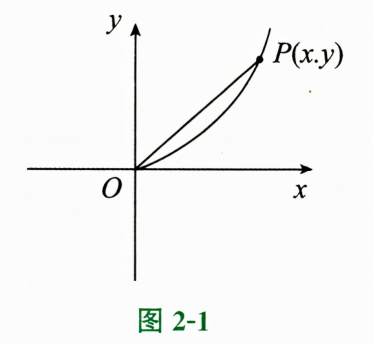
\includegraphics[width=170bp,height=135bp,keepaspectratio]{lilin-figures/第113页.png}

\vfill

\Solution

横坐标、纵坐标和距离都随时间 $t$ 变化，题目给的是 $\frac{\mathrm dx}{\mathrm dt}=30$。由 $9y=4x^2$ 对 $t$ 求导，得 $9\frac{\mathrm dy}{\mathrm dt}=8x\frac{\mathrm dx}{\mathrm dt}$，在 $x=3$ 处 $\frac{\mathrm dy}{\mathrm dt}=80$。

原点到动点的距离满足 $s^2=x^2+y^2$。对 $t$ 求导，并约去系数 $2$，得 $s\frac{\mathrm ds}{\mathrm dt}=x\frac{\mathrm dx}{\mathrm dt}+y\frac{\mathrm dy}{\mathrm dt}$。在 $(3,4)$ 处，$s=5$，所以 $\frac{\mathrm ds}{\mathrm dt}=\frac{3\cdot30+4\cdot80}{5}=82$ 厘米每秒。正号表示点正在远离原点。

\clearpage

% SOURCE line=800 pdf_page=119 section=2.2

\Question{104}{第2章 · 选择题 · 第 6 题}

设 $f(x)=\left\{\begin{aligned}&x^{\alpha}\cdot\cos\frac{1}{x^{\beta}},&x>0,\\&0,&x\leqslant0\end{aligned}\right.$ $(\alpha>0,\beta>0)$，若 $f^{\prime}(x)$ 在 x=0 处连续，则().

\textbf{A.} $\alpha-\beta>1$

\textbf{B.} $0<\alpha-\beta\leq1$

\textbf{C.} $\alpha-\beta>2$

\textbf{D.} $0<\alpha-\beta\leq2$

\vfill

\Solution

左侧函数恒为零，所以若 $f'$ 在 $0$ 连续，必有 $f'(0)=0$。右侧求导时，内层 $x^{-\beta}$ 还要再求导，得到
\[
f'(x)=\alpha x^{\alpha-1}\cos(x^{-\beta})+\beta x^{\alpha-\beta-1}\sin(x^{-\beta}).
\]
第二项的幂次更低。令 $x=(\frac\pi2+2k\pi)^{-\frac1\beta}\to0^+$，则余弦为零、正弦为 $1$。要让导数沿这串点趋于零，必须 $\alpha-\beta-1>0$。此时 $\alpha>1$，右差商 $x^{\alpha-1}\cos(x^{-\beta})\to0$，且导函数上式的两项都趋于零，确实连续。因此选 A。

\clearpage

% SOURCE line=830 pdf_page=122 section=2.2

\Question{105}{第2章 · 填空题 · 第 2 题}

设 $f(x) = x^{3} + x^{2} \cdot |x|$，则 $f(x)$ 的最高阶导数 n = \underline{\hspace{4em}}.

\vfill

\Solution

去绝对值后，函数在 $x\geq0$ 等于 $2x^3$，在 $x<0$ 等于 $0$。分段多项式只需要检查交界 $0$。第一阶和第二阶的右差商分别为 $2x^2$ 和 $6x$，都趋于零，左差商恒为零，因此 $f'(0)=f''(0)=0$。

第二阶导数在 $x>0$ 等于 $12x$，在 $x<0$ 等于 $0$。它在零点的右差商为 $12$、左差商为 $0$，故 $f'''(0)$ 不存在。全定义域上可求的最高阶数为 $2$。

\clearpage

% SOURCE line=834 pdf_page=123 section=2.2

\Question{106}{第2章 · 填空题 · 第 3 题}

设 $f(x)=(x-1)(x-2)\cdots(x-100)$，则 $f'(2)=$ \underline{\hspace{4em}}.

\vfill

\Solution

把恰好在 $x=2$ 为零的因子 $(x-2)$ 单独提出，令其他因子之积为 $G(x)$。乘积求导给出 $f'(2)=G(2)+(2-2)G'(2)=G(2)$。代入剩余因子，
\[
G(2)=(2-1)(2-3)(2-4)\cdots(2-100)=(-1)^{98}\,98!=98!.
\]
数负号时从 $-1$ 到 $-98$ 一共 $98$ 个，所以结果为正。

\clearpage

% SOURCE line=838 pdf_page=124 section=2.2

\Question{107}{第2章 · 填空题 · 第 4 题}

设 $f(x)=\frac{1}{x^{2}-5x+6}$，则 $f^{(n)}(0)=$ \underline{\hspace{4em}}.

\vfill

\Solution

分母有两个线性因子，先拆成部分分式，以免反复用商法则：
\[
f(x)=\frac1{(2-x)(3-x)}=\frac1{2-x}-\frac1{3-x}.
\]
求 $\frac1{a-x}$ 的导数时，幂函数带来的负号与内层导数 $-1$ 抵消。每求导一次分母幂次加一，并把旧幂次乘到分子。故其 $n$ 阶导数是 $\frac{n!}{(a-x)^{n+1}}$，代入 $x=0$ 得
\[
f^{(n)}(0)=n!\left(\frac1{2^{n+1}}-\frac1{3^{n+1}}\right).
\]

\clearpage

% SOURCE line=846 pdf_page=126 section=2.2

\Question{108}{第2章 · 填空题 · 第 6 题}

(仅数学一、数学二要求)已知曲线的极坐标方程为$r=1-\cos\theta$，则该曲线上对应于$\theta=\frac{\pi}{6}$处的切线的直角坐标方程为\_\_\_。

\vfill

\Solution

把极坐标改为参数方程：$x=r\cos\theta$、$y=r\sin\theta$。在 $\theta=\frac\pi6$，$r=1-\frac{\sqrt3}2$，所以 $(x_0,y_0)=(\frac{2\sqrt3-3}{4},\frac{2-\sqrt3}{4})$。

用乘积求导得到 $x_\theta=r'\cos\theta-r\sin\theta$，$y_\theta=r'\sin\theta+r\cos\theta$。代入 $r'=\sin\theta=\frac12$，二者均为 $\frac{\sqrt3-1}{2}$。横坐标导数非零，切线斜率可用 $\frac{y_\theta}{x_\theta}=1$，故切线为 $y-y_0=x-x_0$，即 $y=x+\frac{5-3\sqrt3}{4}$。

\clearpage

% SOURCE line=850 pdf_page=127 section=2.2

\Question{109}{第2章 · 填空题 · 第 7 题}

曲线 $\begin{cases} x = \arctan t, \\ y = \ln \sqrt{1+t^2} \end{cases}$ 上对应于 t = 1 点处的法线方程为\_\_\_。

\vfill

\Solution

先找过点与切线斜率。$t=1$ 时点为 $(\frac\pi4,\frac12\ln2)$。将 $y=\ln\sqrt{1+t^2}$ 写成 $\frac12\ln(1+t^2)$，可得
\[
\frac{\mathrm dx}{\mathrm dt}=\frac1{1+t^2},\qquad \frac{\mathrm dy}{\mathrm dt}=\frac{t}{1+t^2}.
\]
两式相除，切线斜率为 $t$，在 $t=1$ 等于 $1$。法线与切线垂直，所以斜率为 $-1$。所求方程是 $y-\frac12\ln2=-\left(x-\frac\pi4\right)$。

\clearpage

% SOURCE line=856 pdf_page=128 section=2.2

\Question{110}{第2章 · 解答题 · 第 1 题}

求下列函数的导数或微分： (I) $y = \frac{\mathrm{e}^{x} \sin x}{\sqrt{1 + x^2}}$, 求 $y'$; (II) $y = (1 + x^2)^{\sqrt{x}}$ ($x > 0$), 求 $y'$; (III) 设 $y = y(x)$ 由方程 $e^y + xy = e$ 确定，求 $\left. \frac{d^2 y}{dx^2} \right|_{x=0}$; (IV) 设 $x = y^y$, 求 $dy$; (V) (仅数学一、数学二要求) 设 $y = y(x)$ 由 $\left\{\begin{array}{l} x = \arctan t, \\ 2y - ty^2 = 5 - e^t \end{array}\right.$ 确定，求 $\frac{dy}{dx}$; (VI) 设 $y = f\left(\frac{3x - 2}{3x + 2}\right)$, 且 $f'(x) = \arcsin x^2$, 求 $\left. \frac{dy}{dx} \right|_{x=0}$.

\vfill

\Solution

（I）把原式看成三个因子的积：$\mathrm e^x$、$\sin x$、$(1+x^2)^{-\frac12}$，依次只对其中一个求导。合并得 $y'=\frac{\mathrm e^x(\sin x+\cos x)}{\sqrt{1+x^2}}-\frac{x\mathrm e^x\sin x}{(1+x^2)^{\frac32}}$。

（II）底数和指数都变化，先取对数。由 $\ln y=\sqrt{x}\ln(1+x^2)$，用乘积法则得 $y'=y\left[\frac{\ln(1+x^2)}{2\sqrt{x}}+\frac{2x\sqrt{x}}{1+x^2}\right]$。

（III）$x=0$ 时 $y=1$。求导得 $(\mathrm e^y+x)y'=-y$，故 $y'(0)=-\frac1{\mathrm e}$。再求导得 $(\mathrm e^y+x)y''+\mathrm e^y(y')^2+2y'=0$，代入得 $y''(0)=\frac1{\mathrm e^2}$。

（IV）对 $x=y^y$ 取对数，得 $\ln x=y\ln y$（$y>0$）。两边微分得 $\mathrm dy=\frac{\mathrm dx}{x(1+\ln y)}$，适用于 $y\ne\mathrm e^{-1}$。

（V）对参数 $t$ 求导，得 $2(1-ty)y_t=y^2-\mathrm e^t$ 和 $x_t=\frac1{1+t^2}$。相除得 $\frac{\mathrm dy}{\mathrm dx}=\frac{(1+t^2)(y^2-\mathrm e^t)}{2(1-ty)}$（$1-ty\ne0$）。

（VI）内层 $u=\frac{3x-2}{3x+2}$ 满足 $u(0)=-1$、$u'(0)=\frac{12}{(3\cdot0+2)^2}=3$。按链式法则结果为 $3\arcsin 1=\frac{3\pi}{2}$。若只采用题给反正弦公式的实数自然定义域，则 $x=0$ 为端点，这个值对应右导数。若要求双侧导数，需要 $f$ 在 $u=-1$ 两侧可导的条件。

\clearpage

% SOURCE line=866 pdf_page=129 section=2.2

\Question{111}{第2章 · 解答题 · 第 2 题}

求高阶导数：

（I）设 $y = e^{x} \sin x$，求 $y^{(n)}(x)$；

（II）设 $y = x^{2}\ln(1+x)$，求 $y^{(10)}(0)$

（III）设 $f(x)=\frac{5x-1}{2x^{2}+x-1}$，求 $f^{(n)}(0)$.

\vfill

\Solution

（I）先看每求一次导数发生什么。设当前因子是 $\mathrm e^x\sin(x+\phi)$，求导后变成 $\mathrm e^x[\sin(x+\phi)+\cos(x+\phi)]=\sqrt2\,\mathrm e^x\sin(x+\phi+\frac\pi4)$。因此求导 $n$ 次后，系数乘 $(\sqrt2)^n$，相位增加 $\frac{n\pi}{4}$，得到 $y^{(n)}(x)=2^{\frac n2}\mathrm e^x\sin(x+\frac{n\pi}{4})$。

（II）对 $x^2\ln(1+x)$ 用乘积的高阶求导公式。代入 $x=0$ 后，只留下对 $x^2$ 恰求两次导数的项。$\ln(1+x)$ 八阶导数在 $0$ 处为 $-7!$，故 $y^{(10)}(0)=2\binom{10}{2}(-7!)=-\frac{10!}{8}=-453600$。

（III）先把分式拆开，$\frac{5x-1}{(2x-1)(x+1)}=-\frac{1}{1-2x}+\frac{2}{1+x}$。这两个分式求导时，线性内层每次带出固定系数，分母幂次逐次增加。因此 $f^{(n)}(0)=n![-2^n+2(-1)^n]$。

\clearpage

% SOURCE line=876 pdf_page=130 section=2.2

\Question{112}{第2章 · 解答题 · 第 3 题}

设 $f(x)$ 满足 $af(x)+bf\left(\frac{1}{x}\right)=\frac{c}{x}$, $\left|a\right|\neq\left|b\right|$, 求 $f'(x)$.

\vfill

\Solution

等式中有 $f(x)$ 和 $f(\frac1x)$ 两个未知量。把 $x$ 换成 $\frac1x$，两者的位置就交换了，得到联立方程：
\[
af(x)+bf(\frac1x)=\frac cx,\qquad bf(x)+af(\frac1x)=cx.
\]
第一式乘 $a$，第二式乘 $b$，相减消去 $f(\frac1x)$。因为 $a^2-b^2\ne0$，$f(x)=\frac{c}{a^2-b^2}(\frac ax-bx)$。最后按幂函数求导得 $f'(x)=-\frac{c}{a^2-b^2}(\frac a{x^2}+b)$，$x\ne0$。

\clearpage

% SOURCE line=896 pdf_page=134 section=2.2

\Question{113}{第2章 · 解答题 · 第 7 题}

设 $y = y(x)$ 由 $\left\{\begin{array}{l}x = 2t + |t|, \\ y = 5t^2 + 4t |t\end{array}\right.$ 所确定，求 $\left.\frac{dy}{dx}\right|_{t=0}$.

\vfill

\Solution

参数在 $0$ 处带绝对值，分别写两支：$t>0$ 时 $x=3t$、$y=9t^2$；$t<0$ 时 $x=t$、$y=t^2$。所以不论哪一支，都有 $y=x^2$。在 $t=0$ 也有 $(x,y)=(0,0)$，于是 $\left.\frac{\mathrm dy}{\mathrm dx}\right|_{t=0}=2\cdot0=0$。

也可以检查两支的差商。$\frac{y-0}{x-0}$ 分别为 $3t$ 和 $t$，均趋于零。这样可以处理 $x(t)$ 自身在 $t=0$ 不可导的情形。

\clearpage

% SOURCE line=1188 pdf_page=185 section=2.2

\Question{114}{第3章 · 解答题 · 第 14 题}

证明: 当 x > 1 时, 有 $2\arctan x + \arcsin \frac{2x}{1 + x^{2}} = \pi$.

\vfill

\Solution

反三角函数的难点是值域限制。令 $\theta=\arctan x$，由 $x>1$ 得 $\frac\pi4<\theta<\frac\pi2$。二倍角公式给出
\[
\frac{2x}{1+x^2}=\sin2\theta=\sin(\pi-2\theta).
\]
此时 $0<\pi-2\theta<\frac\pi2$，恰好落在 $\arcsin$ 的取值区间 $[-\frac\pi2,\frac\pi2]$ 内，因此 $\arcsin\frac{2x}{1+x^2}=\pi-2\theta$。再加上 $2\arctan x=2\theta$，结果为 $\pi$。

也可通过求导证明等式左侧为常数，但这里用三角恒等式能直接解释为什么常数恰为 $\pi$。

\clearpage

% SOURCE line=2197 pdf_page=353 section=2.2

\Question{115}{第7章 · 解答题 · 第 3 题}

某商品的需求量 $Q = Q(P)$，需求对价格的弹性 $\eta = \frac{2P^{2}}{192 - P^{2}}$，若 R 为总收益函数，证明：$\frac{dR}{dP} = Q(1 - \eta)$.

\vfill

\Solution

单价为 $P$、销量为 $Q(P)$ 时，总收益为 $R(P)=P Q(P)$。需求弹性的定义是 $\eta=-\frac{P}{Q}\frac{\mathrm dQ}{\mathrm dP}$，其中负号使价格升高、销量降低的需求对应正值。

因为两个乘数都随 $P$ 变化，要用乘积法则。计算得
\[
\frac{\mathrm dR}{\mathrm dP}=Q+P\frac{\mathrm dQ}{\mathrm dP}=Q\left(1+\frac P Q\frac{\mathrm dQ}{\mathrm dP}\right)=Q(1-\eta).
\]
代入题给表达式还可写成 $\frac{\mathrm dR}{\mathrm dP}=Q\frac{192-3P^2}{192-P^2}$。题目所要证明的恒等式直接来自收入定义与乘积求导法则。

\clearpage

% SOURCE line=2317 pdf_page=375 section=2.2

\Question{116}{第8章 · 例题第3组 · 例 6}

设由方程组 $\left\{\begin{array}{l}x+y+z=0,\\x^{2}+y^{2}+z^{2}=1\end{array}\right.$ 确定 $x=x(z), y=y(z)$，求 $\frac{dx}{dz}$，$\frac{dy}{dz}$。

\vfill

\Solution

虽然三个字母同时出现，题中只有一个自变量 $z$，$x,y$ 都是它的函数。因此只需要一元函数的隐函数求导，逐式对 $z$ 求导即可。第一条给 $x'+y'=-1$；第二条用平方函数的链式法则，除以 $2$ 后得到 $xx'+yy'=-z$。

把第一式乘 $y$，从第二式减去它，消去 $y'$，得 $(x-y)x'=y-z$。再由 $y'=-1-x'$ 求出另一项：
\[
\frac{\mathrm dx}{\mathrm dz}=\frac{y-z}{x-y},\qquad
\frac{\mathrm dy}{\mathrm dz}=\frac{z-x}{x-y}.
\]
这里 $x\ne y$。若 $x=y$，导数方程要求 $z=x$，再用原方程 $x+y+z=0$ 得三者为零，与平方和为 $1$ 矛盾。因此这些点不存在题中所要求的有限导数，应作为分支端点处理。

\clearpage

% SOURCE line=2487 pdf_page=405 section=2.2

\Question{117}{第8章 · 填空题 · 第 3 题}

已知 $y = y(x)$, $z = z(x)$ 由方程组 $\left\{\begin{aligned}z &= x^{2} + y^{2},\\ x^{2} + 2y^{2} + 3z^{2} &= 20\end{aligned}\right.$ 确定，则 $\frac{dy}{dx} =$ \underline{\hspace{4em}} , $\frac{dz}{dx} =$ \underline{\hspace{4em}}.

\vfill

\Solution

把 $y,z$ 当作 $x$ 的函数，每次对它们的平方求导都要带上自身的导数。由两条方程分别得
\[
z'=2x+2yy',\qquad 2x+4yy'+6zz'=0.
\]
代入第一式消去 $z'$，整理得到 $2x(1+6z)+4y(1+3z)y'=0$。所以
\[
\frac{\mathrm dy}{\mathrm dx}
=-\frac{x(1+6z)}{2y(1+3z)},\qquad
\frac{\mathrm dz}{\mathrm dx}=\frac{x}{1+3z}.
\]
第二式由 $2x+2yy'$ 化简而得。原条件 $z=x^2+y^2\ge0$ 保证 $1+3z>0$。若 $y=0$，原方程给 $x\ne0$，上述两条导数关系将互相矛盾，所以两函数能同时可导的分支要求 $y\ne0$。

\clearpage

% SOURCE line=2726 pdf_page=456 section=2.2

\Question{118}{第9章 · 例题第3组 · 例 12}

（数学三不要求）设函数 $y=f(x)$ 由参数方程 $\left\{\begin{aligned}x=2t+t^{2},\\ y=\varphi(t)\end{aligned}\right.$ （$t>-1$）确定，$\varphi(t)$ 具有二阶导数，且 $\varphi(1)=\frac{5}{2}$，$\varphi'(1)=6$，已知 $\frac{d^{2}y}{dx^{2}}=\frac{3}{4(1+t)}$，求 $\varphi(t)$.

\vfill

\Solution

已知的是对 $x$ 的二阶导数，但待求的是 $t$ 的函数。先令 $p(t)=\frac{\mathrm dy}{\mathrm dx}$。因 $x'(t)=2(1+t)>0$，链式法则给出
\[
p'(t)=\frac{\mathrm d^2y}{\mathrm dx^2}\,x'(t)=\frac32.
\]
初值 $p(1)=\frac{\varphi'(1)}{x'(1)}=\frac64=\frac32$，所以 $p(t)=\frac32t$。再由 $\varphi'(t)=p(t)x'(t)=3t(1+t)$ 积分，得 $\varphi(t)=t^3+\frac32t^2+C$。

用 $\varphi(1)=\frac52$ 得 $C=0$。反代有 $\frac{\mathrm d^2y}{\mathrm dx^2}=\frac{\frac32}{2(1+t)}$，与题设一致。

\clearpage

\SectionHeading{2.3}{微分}

% SOURCE line=573 pdf_page=88 section=2.3

\Question{119}{第2章 · 例题第1组 · 例 7}

设函数 $f(u)$ 可导, $y = f(x^{2})$, 当自变量 x 在 x = -1 处取得增量 $\Delta x = -0.1$ 时, 相应的函数增量 $\Delta y$ 的线性主部为 0.1, 则 $f'(1) = (\quad)$.

\textbf{A.} 1

\textbf{B.} 0.1

\textbf{C.} 0.2

\textbf{D.} 0.5

\vfill

\Solution

“增量的线性主部”就是 $\mathrm dy=y'(x)\Delta x$，意思是只保留关于 $\Delta x$ 的一次项。对 $y=f(x^2)$ 先对外层求导，再乘里层 $x^2$ 的导数 $2x$，所以 $y'=2xf'(x^2)$。

代入 $x=-1$ 和 $\Delta x=-0.1$，得 $0.1=(-2)f'(1)\cdot(-0.1)=0.2f'(1)$。因此 $f'(1)=0.5$，选 D。

\clearpage

% SOURCE line=681 pdf_page=102 section=2.3

\Question{120}{第2章 · 例题第2组 · 例 3}

设 $y = y(x)$ 由方程 $2^{xy} = x + y$ 确定，求 $\mathrm{d}y\big|_{x=0}$.

\vfill

\Solution

要求的是微分，所以目标是先求该点的 $y'$，再乘 $\mathrm dx$。令 $x=0$，原式给出 $y=1$。两边对 $x$ 求导，左边按复合函数处理：
\[
2^{xy}\ln 2\,(y+xy')=1+y'.
\]
在 $(0,1)$ 处，左边只剩 $\ln 2$，故 $y'=\ln2-1$，从而 $\left.\mathrm dy\right|_{x=0}=(\ln2-1)\,\mathrm dx$。

\clearpage

% SOURCE line=2205 pdf_page=355 section=2.3

\Question{121}{第7章 · 解答题 · 第 5 题}

设某产品的需求函数 $Q = Q(P)$，其对价格 P 的弹性 $\xi_{P} = 0.2$，当需求量为 10000 件时，价格增加 1 元，问此时会使产品的收益增加多少元？

\vfill

\Solution

收入等于单价乘需求量，$R(P)=P Q(P)$，用乘积法则得 $R'=Q+PQ'$。本题没有写明符号 $\xi_P$ 的定义，计算时须说明约定。

若采用需求价格弹性的正值约定 $\xi_P=-\frac{P}{Q}Q'$，则 $R'=Q(1-\xi_P)=10000\times0.8=8000$。由微分估计，价格增加 $1$ 元，收入约增加 $8000$ 元。

若 $\xi_P$ 采用一般函数的有符号弹性定义 $\xi_P=\frac{P}{Q}Q'$，则 $R'=Q(1+\xi_P)=12000$，收入约增加 $12000$ 元。两种符号定义相差一个负号，需与原讲义的定义核对。两者都是当前价格处的微分估计；题面未给完整需求函数，无法确定涨价一元后的精确收入差额。

\clearpage

% SOURCE line=2213 pdf_page=357 section=2.3

\Question{122}{第7章 · 解答题 · 第 7 题}

设某商品需求函数为 Q = 100 - 5P.

（I）当 P = 3 时，问涨价会使销售收入增加还是减少？若价格上涨幅度为 8.5\%，则对销售收入的影响幅度为多少？

（II）当P=12时，问涨价会使销售收入增加还是减少？若价格上涨幅度为5\%，则对销售收入影响的幅度为多少？

\vfill

\Solution

收入为 $R(P)=P(100-5P)$，导数为 $R'(P)=100-10P$。在 $P=3$ 时导数为正，涨价增加收入；在 $P=12$ 时为负，涨价减少收入。

若用微分估计相对变化，$\frac{\mathrm dR}{R}=\frac{20-2P}{20-P}\frac{\mathrm dP}{P}$。因此（I）约增加 $\frac{14}{17}\times8.5\%=7\%$；（II）约减少 $\frac12\times5\%=2.5\%$。

本题给出了完整需求函数，还能求精确幅度。若涨价比例为 $\varepsilon$，直接把新价格 $P(1+\varepsilon)$ 代入收入函数，得到 $\frac{\Delta R}{R}=\frac{20-2P}{20-P}\varepsilon-\frac{P}{20-P}\varepsilon^2$。代入（I）的 $P=3,\varepsilon=0.085$，精确增加 $6.8725\%$；代入（II）的 $P=12,\varepsilon=0.05$，精确减少 $2.875\%$。微分估计忽略了这个二次项。

\clearpage

\SectionHeading{2.4}{微分中值定理及其应用}

% SOURCE line=902 pdf_page=135 section=2.4

\Question{123}{第3章 · 示例 · 示例}

若 $f(x)=2^{x}-x^{2}-1,x\in(-\infty,+\infty),\quad f'''(x)=2^{x}(\ln2)^{3}\neq0$ 则 $f(x)=2^{x}-x^{2}-1=0$ 至多有三个实根.

\vfill

\Solution

题中已经告诉我们 $f'''$ 处处不为零，说明应设法把 $f$ 的多个零点转化成一个三阶导数的零点。Rolle 定理恰好能把同一个函数的两个不同零点变成它们之间的一个导数零点。

反设 $f$ 有四个不同零点 $x_1<x_2<x_3<x_4$。分别在三个相邻区间用 Rolle 定理，$f'$ 至少有三个不同零点。再对 $f'$ 的两个相邻零点区间各用一次，$f''$ 至少有两个不同零点。最后在这两个点之间对 $f''$ 用 Rolle 定理，得到一点 $c$ 使 $f'''(c)=0$。

但直接求导得 $f'''(c)=2^c(\ln2)^3>0$，矛盾。所以原方程至多有三个不同实根。这里各次使用定理所需的连续、可导都由 $2^x-x^2-1$ 的光滑性保证。

\clearpage

% SOURCE line=912 pdf_page=136 section=2.4

\Question{124}{第3章 · 例题第1组 · 例 1}

设 $f(x)$ 在 $[0,1]$ 上有二阶导数，$f(x)$ 不恒为 0，且曲线 $y = f(x)$ 的端点连线与曲线相交于 C 点，证明：至少存在一点 $\xi \in (0,1)$，使 $f''(\xi) = 0$。

\vfill

\Solution

设端点弦的方程为 $L(x)=f(0)+[f(1)-f(0)]x$。把曲线减去这条直线，交点就变成零点，而且 $L''=0$，不会改变要求的二阶导数。

设内部交点 $C$ 的横坐标为 $c\in(0,1)$，令 $F=f-L$。于是 $F(0)=F(c)=F(1)=0$。分别在 $[0,c]$ 和 $[c,1]$ 用 Rolle 定理，得到 $u\in(0,c)$、$v\in(c,1)$，满足 $F'(u)=F'(v)=0$。

再对 $F'$ 在 $[u,v]$ 用 Rolle 定理，得到 $\xi$ 使 $F''(\xi)=0$，即 $f''(\xi)=0$。题中交点 $C$ 需理解为异于两个端点；只把端点算成交点时结论不成立。

\clearpage

% SOURCE line=916 pdf_page=137 section=2.4

\Question{125}{第3章 · 例题第1组 · 例 2}

设 $f(x)$ 在 $[0,1]$ 上连续，在 $(0,1)$ 内可导，且 $f(1)=2f(0)$，证明：至少存在一点 $\xi\in(0,1)$，使得 $(1+\xi)f'(\xi)=f(\xi)$.

\vfill

\Solution

目标的左边可以写成 $(1+x)f'(x)-f(x)$。看到“一项是 $f'$，一项是 $-f$”，试回忆商的求导公式：
\[
\left(\frac{f(x)}{1+x}\right)'=\frac{(1+x)f'(x)-f(x)}{(1+x)^2}.
\]
设 $F(x)=\frac{f(x)}{1+x}$。分母全区间为正，故 $F$ 闭区间连续、开区间可导。又 $F(0)=f(0)$，$F(1)=\frac{f(1)}2=f(0)$，正好满足 Rolle 定理的端点相等条件。

于是存在 $\xi\in(0,1)$ 使 $F'(\xi)=0$，将上面的正分母乘过去，即得 $(1+\xi)f'(\xi)=f(\xi)$。

\clearpage

% SOURCE line=920 pdf_page=138 section=2.4

\Question{126}{第3章 · 例题第1组 · 例 3}

设 $f(x)$ 在 $[0,1]$ 上连续，在 $(0,1)$ 内可导，$f(0)=0$，证明：至少存在一点 $\xi\in(0,1)$，使得 $\xi f'(\xi)+nf(\xi)=f'(\xi)$（$n$ 为正整数）.

\vfill

\Solution

把目标改写成 $(1-x)f'(x)-nf(x)=0$。因为 $(1-x)^n$ 的导数为 $-n(1-x)^{n-1}$，乘积求导正好会同时出现这两项。令 $F(x)=(1-x)^n f(x)$。

$F(0)=f(0)=0$，且 $n$ 为正整数，保证 $F(1)=0$。由连续与可导的条件，可以在 $[0,1]$ 对 $F$ 用 Rolle 定理。因此某个 $\xi\in(0,1)$ 满足
\[
0=F'(\xi)=(1-\xi)^{n-1}\bigl[(1-\xi)f'(\xi)-nf(\xi)\bigr].
\]
因 $\xi<1$，外面的因子严格为正，约去后即得题设关系。

\clearpage

% SOURCE line=924 pdf_page=139 section=2.4

\Question{127}{第3章 · 例题第1组 · 例 4}

设 $f(x)$ 在 $[0,1]$ 上连续，在 $(0,1)$ 内可导，且 $f(0) = f(1) = 0$，$f\left(\frac{1}{2}\right) = 1$，证明：

(1) 至少存在一点 $\eta \in \left(\frac{1}{2}, 1\right)$，使得 $f(\eta) = \eta$;

(2) 对任意实数 $\lambda$，至少存在一点 $\xi \in (0, \eta)$，使得 $f'(\xi) - \lambda [f(\xi) - \xi] = 1$.

\vfill

\Solution

（1）比较 $f(x)$ 和 $x$，先设 $g(x)=f(x)-x$。有 $g(\frac12)=\frac12>0$，$g(1)=-1<0$。由于 $g$ 连续，介值定理给出 $\eta\in(\frac12,1)$，使 $g(\eta)=0$。

（2）目标整理成 $g'(\xi)-\lambda g(\xi)=0$。要把减去常数倍这一结构变成一个导数，给 $g$ 乘 $\mathrm e^{-\lambda x}$。令 $G(x)=\mathrm e^{-\lambda x}g(x)$，其在 $0,\eta$ 的值都是零。

由 Rolle 定理，存在 $\xi\in(0,\eta)$ 使 $G'(\xi)=\mathrm e^{-\lambda\xi}[g'(\xi)-\lambda g(\xi)]=0$。指数因子为正，代回 $g=f-x$ 即得 $f'(\xi)-\lambda[f(\xi)-\xi]=1$。这个构造对任意实数 $\lambda$ 都有效。

\clearpage

% SOURCE line=932 pdf_page=140 section=2.4

\Question{128}{第3章 · 例题第1组 · 例 5}

设奇函数 $f(x)$ 在 $[-1,1]$ 上二阶可导，且 $f(1)=1$，证明：

(1) 至少存在一点 $\xi \in (0,1)$，使得 $f'(\xi) = 1$.

(2) 至少存在一点 $\eta \in (-1,1)$，使得 $f''(\eta) + f'(\eta) = 1$.

\vfill

\Solution

（1）奇性给出 $f(0)=0$。在 $[0,1]$ 用 Lagrange 中值定理，某个 $\xi\in(0,1)$ 的导数等于端点割线斜率，故 $f'(\xi)=\frac{1-0}{1-0}=1$。

（2）对 $f(-x)=-f(x)$ 求导得到 $f'(-x)=f'(x)$，所以 $f'(\xi)-1$ 和 $f'(-\xi)-1$ 都为零。目标是 $f''+f'-1=0$，它来自 $f'-1$ 与指数函数的乘积求导。

令 $F(x)=\mathrm e^x[f'(x)-1]$，在 $[-\xi,\xi]$ 对它用 Rolle 定理。所得 $\eta$ 满足 $0=F'(\eta)=\mathrm e^\eta[f''(\eta)+f'(\eta)-1]$。约去非零指数因子便得结论。

\clearpage

% SOURCE line=940 pdf_page=141 section=2.4

\Question{129}{第3章 · 例题第1组 · 例 6}

设 $f(x)$ 在 $[0,1]$ 上二阶可导，且 $f(1) > 0$，$\lim_{x \to 0^{+}} \frac{f(x)}{x} < 0$。证明：

(1) 方程 $f(x) = 0$ 在 $(0,1)$ 内至少有一个实根；

(2) 方程 $f(x)f''(x) + [f'(x)]^2 = 0$ 在 $(0,1)$ 内至少有两个不同实根.

\vfill

\Solution

（1）题给 $\frac{f(x)}x$ 的右极限为有限负数，因而 $f(0)=0$，并且存在充分小的 $t>0$ 使 $f(t)<0$。结合 $f(1)>0$，由介值定理，在 $(t,1)$ 内有根 $c$。

（2）目标左边等于 $\bigl(\frac12f^2\bigr)''$，因为先求一次导数得 $ff'$。记 $F=\frac12f^2$。由 $f(0)=f(c)=0$ 可知 $F'(0)=F'(c)=0$，并由 Rolle 定理在 $(0,c)$ 内找到 $u$ 使 $F'(u)=0$。

现在对 $F'$ 在 $[0,u]$ 和 $[u,c]$ 各用一次 Rolle 定理，各得一个 $F''$ 的零点。两个开区间互不重叠，所以两点不同。有限性不可省略：若把负无穷也允许，$f(x)=x-\frac12$ 会使第二问不成立。

\clearpage

% SOURCE line=948 pdf_page=142 section=2.4

\Question{130}{第3章 · 例题第1组 · 例 7}

设 $f(x)$ 在 $[0,1]$ 上二阶可导，且 $\lim_{x\to0^{+}}\frac{f(x)}{x}=0$，$\lim_{x\to1^{-}}\frac{f(x)-1}{x-1}=1$，证明：至少存在一点 $\xi\in(0,1)$，使得 $f''(\xi)=f(\xi)$。

\vfill

\Solution

有限的两个差商极限先给出 $f(0)=0$、$f(1)=1$；再按端点导数定义得到 $f'(0)=0$、$f'(1)=1$。因此 $f'(0)-f(0)=f'(1)-f(1)=0$，有了两个相等的端点值。

目标是 $f''-f=0$。取 $G(x)=\mathrm e^x[f'(x)-f(x)]$，这样对指数求导产生的 $+f'$ 与对括号求导产生的 $-f'$ 抵消：
\[
G'(x)=\mathrm e^x[f''(x)-f(x)].
\]
因为 $G(0)=G(1)=0$，由 Rolle 定理可取 $\xi\in(0,1)$ 使 $G'(\xi)=0$。指数因子为正，故 $f''(\xi)=f(\xi)$。

\clearpage

% SOURCE line=952 pdf_page=143 section=2.4

\Question{131}{第3章 · 例题第1组 · 例 8}

设 $f(x), g(x)$ 在 $[a, b]$ 上存在二阶导数, $g''(x) \neq 0$, 且 $f(a) = f(b) = g(a) = g(b) = 0$, 证明: 至少存在一点 $\xi \in (a, b)$, 使得 $\frac{f(\xi)}{g(\xi)} = \frac{f''(\xi)}{g''(\xi)}$.

\vfill

\Solution

先保证分式有意义。若 $g$ 在 $(a,b)$ 另有一个零点，由两次 Rolle 定理，$g''$ 会有一个零点，与题设矛盾。因此 $g$ 在开区间处处非零。

目标交叉相乘是 $f''g-fg''=0$，看见它是 $H(x)=f'(x)g(x)-f(x)g'(x)$ 的导数，因为中间两项 $f'g'$ 正好抵消。

已知两函数在端点都为零，所以 $H(a)=H(b)=0$。对 $H$ 用 Rolle 定理，存在 $\xi\in(a,b)$ 使 $f''(\xi)g(\xi)-f(\xi)g''(\xi)=0$。此处 $g(\xi)$ 与 $g''(\xi)$ 都非零，除以它们的乘积即得所证。

\clearpage

% SOURCE line=956 pdf_page=144 section=2.4

\Question{132}{第3章 · 例题第1组 · 例 9}

设 $f(x)$ 在 $[0,1]$ 上连续，在 $(0,1)$ 内可导，且满足 $f(1)=k\int_{0}^{\frac{1}{k}}x\mathrm{e}^{1-x}f(x)\mathrm{d}x$，$k>1$，

证明：至少存在一点 $\xi\in(0,1)$，使得 $f^{\prime}(\xi)=(1-\xi^{-1})f(\xi)$.

\vfill

\Solution

目标乘以 $\xi$ 后是 $xf'(x)+(1-x)f(x)=0$，它正出现在 $F(x)=x\mathrm e^{1-x}f(x)$ 的导数中。题给的积分也正是 $F$ 的积分。

因为 $F(1)=f(1)$，题意是 $F(1)=k\int_0^{\frac1k}F(x)\,\mathrm dx$，即 $F(1)$ 等于 $F$ 在 $[0,\frac1k]$ 的平均值。由积分中值定理，在该区间上有一点 $c$ 使 $F(c)=F(1)$。又 $c\le\frac1k<1$，可以在 $[c,1]$ 对 $F$ 用 Rolle 定理。

于是某个 $\xi\in(c,1)$ 满足 $0=F'(\xi)=\mathrm e^{1-\xi}[\xi f'(\xi)+(1-\xi)f(\xi)]$。除以正数 $\xi\mathrm e^{1-\xi}$，得到 $f'(\xi)=(1-\frac1\xi)f(\xi)$。

\clearpage

% SOURCE line=962 pdf_page=145 section=2.4

\Question{133}{第3章 · 例题第1组 · 例 10}

设 $f(x)$ 在 $[a,b]$ 上连续，在 $(a,b)$ 内可导，且 $f(a)=a$，$\int_{a}^{b}f(x)dx=\frac{1}{2}(b^{2}-a^{2})$，证明：

(1) 存在 $c \in (a, b)$，使得 $f(c) = c$.

(2) 存在 $\xi \in (a, c)$，使得 $f'(\xi) = f(\xi) - \xi + 1$.

\vfill

\Solution

（1）把目标设为 $g(x)=f(x)-x$ 的零点。因 $\int_a^b x\,\mathrm dx=\frac12(b^2-a^2)$，题设给 $\int_a^b g(x)\,\mathrm dx=0$。由积分中值定理，某个 $c\in(a,b)$ 满足 $g(c)=0$。若 $g$ 恒为零，可任取内点；若不恒为零，零平均要求它取正值和负值，连续性保证一个内点零点。

（2）目标整理为 $g'(\xi)-g(\xi)=0$，可令 $G(x)=\mathrm e^{-x}g(x)$。有 $g(a)=g(c)=0$，故由 Rolle 定理，在 $(a,c)$ 内有 $\xi$ 使 $G'(\xi)=\mathrm e^{-\xi}[g'(\xi)-g(\xi)]=0$。

代回 $g=f-x$，即 $f'(\xi)-1=f(\xi)-\xi$。

\clearpage

% SOURCE line=972 pdf_page=146 section=2.4

\Question{134}{第3章 · 例题第2组 · 例 1}

证明: 不等式 $\frac{1}{n+1} < \ln(1 + \frac{1}{n}) < \frac{1}{n}$.

\vfill

\Solution

看到 $\ln(1+\frac1n)$，把它写成 $\ln(n+1)-\ln n$。这就成了同一个函数在两个端点的差，而区间长度为 $1$。

对 $g(x)=\ln x$ 在 $[n,n+1]$ 用 Lagrange 中值定理（$n$ 为正整数），得某个 $\xi\in(n,n+1)$，使
\[
\ln\left(1+\frac1n\right)=g'(\xi)(n+1-n)=\frac1\xi.
\]
正数取倒数时大小次序反转，故 $\frac1{n+1}<\frac1\xi<\frac1n$。两个不等式都严格，因为 $\xi$ 在开区间内。

\clearpage

% SOURCE line=976 pdf_page=147 section=2.4

\Question{135}{第3章 · 例题第2组 · 例 2}

设 $x \in [0,1]$, $f''(x) > 0$, 则下列选项正确的是().

\textbf{A.} $f^{\prime}(1) > f^{\prime}(0) > f(1) - f(0)$

\textbf{B.} $f^{\prime}(1) > f(1) - f(0) > f^{\prime}(0)$

\textbf{C.} $f(1) - f(0) > f^{\prime}(1) > f^{\prime}(0)$

\textbf{D.} $f^{\prime}(1) > f(0) - f(1) > f^{\prime}(0)$

\vfill

\Solution

选 B。$f''>0$ 表示 $f'$ 严格增加。理由是任取 $u<v$，对 $f'$ 使用 Lagrange 中值定理，$f'(v)-f'(u)=f''(w)(v-u)>0$。

再看中间可能出现的 $f(1)-f(0)$，它是 $f$ 在整个区间上的割线斜率。对 $f$ 在 $[0,1]$ 用中值定理，得到某个 $\xi\in(0,1)$ 使 $f(1)-f(0)=f'(\xi)$。

把 $\xi$ 处的导数放进递增顺序，即 $f'(0)<f(1)-f(0)<f'(1)$，只有 B 的顺序相符。

\clearpage

% SOURCE line=988 pdf_page=148 section=2.4

\Question{136}{第3章 · 例题第2组 · 例 3}

设定义在$[0,1]$上的可微函数$f(x)$满足$f'(x)\geqslant M>0$，证明：存在$[0,1]$上的一个子区间$I$，若其长度为$\frac{1}{4}$，对$x\in I$，有$|f(x)|\geqslant\frac{1}{4}M$。

\vfill

\Solution

导数至少为 $M$，意味着向右走长度 $\ell$，函数值至少增加 $M\ell$。准确地说，对任意 $u<v$ 用 Lagrange 中值定理可得 $f(v)-f(u)\ge M(v-u)$。

看中点 $\frac12$ 的符号。若 $f(\frac12)\ge0$，对每个 $x\in[\frac34,1]$ 都有 $f(x)\ge f(\frac12)+M(x-\frac12)\ge\frac14M$，取这个右端区间即可。

若 $f(\frac12)<0$，对每个 $x\in[0,\frac14]$ 都有 $f(x)\le f(\frac12)-M(\frac12-x)\le-\frac14M$，取左端区间。两个区间长度都为 $\frac14$，所选区间上 $|f(x)|\ge\frac14M$。

\clearpage

% SOURCE line=992 pdf_page=149 section=2.4

\Question{137}{第3章 · 例题第2组 · 例 4}

设 $f(x)$ 在 $[a,b]$ 上连续，在 $(a,b)$ 内可导，且 $f(a)=f(b)=1$。证明：存在点 $\xi, \eta \in (a,b)$，使得 $\mathrm{e}^{\eta-\xi}[f(\eta)+f'(\eta)]=1$。

\vfill

\Solution

目标等价于 $\mathrm e^\eta[f(\eta)+f'(\eta)]=\mathrm e^\xi$。左边正是 $(\mathrm e^xf(x))'$ 在 $\eta$ 的值，右边是 $(\mathrm e^x)'$ 在 $\xi$ 的值。于是只需让这两个函数的某处导数相等。

令 $F(x)=\mathrm e^xf(x)$、$G(x)=\mathrm e^x$。因为 $f(a)=f(b)=1$，两函数在两个端点分别取相同值，故割线斜率相同。对 $F$ 和 $G$ 分别用 Lagrange 中值定理，得内点 $\eta,\xi$ 使
\[
F'(\eta)=\frac{F(b)-F(a)}{b-a}
=\frac{G(b)-G(a)}{b-a}=G'(\xi).
\]
代入导数并除以 $\mathrm e^\xi$ 即得结论。

\clearpage

% SOURCE line=996 pdf_page=150 section=2.4

\Question{138}{第3章 · 例题第2组 · 例 5}

设 $f(x)$ 在 $[0,1]$ 上连续，在 $(0,1)$ 内可导，且 $f(0)=0, f(1)=1$，证明：

(1) 至少存在一点 $\xi \in (0,1)$，使得 $f(\xi) = 1 - \xi$.

(2) 至少存在不同的两点 $\xi_{1}, \xi_{2} \in (0,1)$，使得 $f^{\prime}(\xi_{1})f^{\prime}(\xi_{2}) = 1$.

\vfill

\Solution

（1）令 $g(x)=f(x)+x-1$，有 $g(0)=-1$、$g(1)=1$。由连续性，介值定理给出 $\xi\in(0,1)$ 使 $g(\xi)=0$，即 $f(\xi)=1-\xi$。

（2）第一问的 $\xi$ 把两段的水平长度和竖直增量交换了，正好得到互为倒数的割线斜率。对 $[0,\xi]$ 用中值定理，存在 $\xi_1\in(0,\xi)$ 使 $f'(\xi_1)=\frac{1-\xi}{\xi}$。对 $[\xi,1]$ 同理得 $\xi_2\in(\xi,1)$，使 $f'(\xi_2)=\frac{\xi}{1-\xi}$。

相乘为 $1$，且两个开区间不相交，故两点不同。

\clearpage

% SOURCE line=1004 pdf_page=151 section=2.4

\Question{139}{第3章 · 例题第2组 · 例 6}

设 $f(x)$ 在 $[0,1]$ 上连续，在 $(0,1)$ 内可导，且 $f(0)=1, f(1)=\mathrm{e}$，证明：存在 $\xi \in \left(0, \frac{1}{2}\right)$，$\eta \in \left(\frac{1}{2}, 1\right)$，使得 $f'(\xi) + f'(\eta) = \mathrm{e}^{\xi} + \mathrm{e}^{\eta}$。

\vfill

\Solution

把目标中两项指数挪到导数旁边，得到 $[f'(\xi)-\mathrm e^\xi]+[f'(\eta)-\mathrm e^\eta]=0$。这提示令 $g(x)=f(x)-\mathrm e^x$，求的是两处 $g'$ 相加为零。

已知 $g(0)=g(1)=0$。在两个等长区间 $[0,\frac12]$ 与 $[\frac12,1]$ 分别用 Lagrange 中值定理，得
\[
g'(\xi)=2g\left(\frac12\right),\qquad
g'(\eta)=-2g\left(\frac12\right).
\]
两段共享中点，端点差恰好相反，因此相加等于零。把 $g'$ 展开便得原式。

\clearpage

% SOURCE line=1008 pdf_page=152 section=2.4

\Question{140}{第3章 · 例题第2组 · 例 7}

设 $f(x)$ 在 $[0,1]$ 上可导，且 $f(0)=0, f(1)=1$，证明：在 $(0,1)$ 内存在 $\xi, \eta$，使得 $\frac{1}{f'(\xi)} + \frac{1}{f'(\eta)} = 2$。

\vfill

\Solution

题目要两个导数的倒数相加。割线斜率的倒数是“水平长度除以竖直增量”。要让相加时分子能拼成总长 $1$，就把竖直增量分成相等的两半。

由 $f(0)=0,f(1)=1$ 和连续性，可取 $c\in(0,1)$ 使 $f(c)=\frac12$。分别对 $[0,c]$ 和 $[c,1]$ 用 Lagrange 中值定理，得
\[
f'(\xi)=\frac{1}{2c},\qquad
f'(\eta)=\frac{1}{2(1-c)}.
\]
这两个导数都为正且不为零，倒数相加为 $2c+2(1-c)=2$。两点分别在两侧，所以还可保证它们不同。

\clearpage

% SOURCE line=1012 pdf_page=153 section=2.4

\Question{141}{第3章 · 例题第2组 · 例 8}

设 $f(x)$ 在 $[a,b]$ 上二阶可导，且 $f(a) > 0, f(b) > 0, \int_{a}^{b} f(x) \, dx = 0$。证明：

(1) 存在相异的 $\xi_{1}, \xi_{2} \in (a, b)$，使得 $f(\xi_{1}) = f(\xi_{2}) = 0$;

(2) 存在一点 $\xi \in (a, b)$，使得 $f''(\xi) > 0$.

\vfill

\Solution

（1）两端函数值为正，连续性保证两端附近都有一段正面积。若全区间 $f\ge0$，总积分就会大于零。因此存在 $c\in(a,b)$ 使 $f(c)<0$。分别在 $[a,c]$ 与 $[c,b]$ 用介值定理，各得一个内点零点。

（2）两端比 $f(c)$ 高，意味着从左到中间的割线斜率为负，从中间到右的割线斜率为正。由 Lagrange 中值定理，存在 $u\in(a,c)$ 使 $f'(u)<0$，存在 $v\in(c,b)$ 使 $f'(v)>0$。

再对 $f'$ 在 $[u,v]$ 用中值定理，得 $\xi\in(u,v)$ 使 $f''(\xi)=\frac{f'(v)-f'(u)}{v-u}>0$。这个步骤把斜率的增加变成了二阶导数的正号。

\clearpage

% SOURCE line=1028 pdf_page=155 section=2.4

\Question{142}{第3章 · 例题第2组 · 例 10}

设 $f(x)$ 在 $[0,1]$ 上有二阶导数，且 $f(0)=0, f(1)=1, \int_{0}^{1} f(x) \, dx = 1$.

(1) 证明：至少存在一点 $\xi \in (0,1)$，使得 $f'(\xi) = 0$;

(2) 证明：至少存在一点 $\eta \in (0,1)$，使得 $f''(\eta) < -2$.

\vfill

\Solution

（1）若 $f(x)\le1$ 在全区间成立，由于 $f(0)=0$，零点附近存在一段使 $f(x)<1$，积分必小于 $1$。所以某个内点 $c$ 有 $f(c)>1$。连续函数的最大值于是取在内部，因为两个端点值都小于 $f(c)$；在最大值点由 Fermat 定理有 $f'(\xi)=0$。

（2）反设处处 $f''\ge-2$。令 $g=f+x^2$，则 $g''\ge0$，它的弧在端点连线下方。具体地，用中值定理比较 $[0,x]$ 与 $[x,1]$ 的割线斜率，因 $g'$ 不减，前者不大于后者。

由 $g(0)=0,g(1)=2$ 得 $g(x)\le2x$，即 $f(x)\le2x-x^2$。积分得 $\int_0^1f\le\frac23<1$，矛盾。因此某个内点有 $f''(\eta)<-2$。

\clearpage

% SOURCE line=1038 pdf_page=156 section=2.4

\Question{143}{第3章 · 例题第3组 · 例 1}

设 $f(x)$ 在 $[a,b]$ 上连续，在 $(a,b)$ 内可导，$0 < a < b$，证明：存在一点 $\xi \in (a,b)$，使得 $\frac{ab}{b-a}[bf(b)-af(a)] = \xi^2[f(\xi) + \xi f'(\xi)]$.

\vfill

\Solution

右边含 $f(x)+xf'(x)$，正是 $(xf(x))'$。还多乘了 $x^2$，可把它理解为除以一个形如 $\frac1{x^2}$ 的导数。取 $F(x)=xf(x)$，$G(x)=-\frac1x$。

因为 $a>0$，两函数都连续可导且 $G'(x)=\frac1{x^2}>0$。用 Cauchy 中值定理得到某个 $\xi\in(a,b)$，使
\[
\frac{F(b)-F(a)}{G(b)-G(a)}=\frac{F'(\xi)}{G'(\xi)}.
\]
左边的分母是 $\frac{b-a}{ab}$，右边是 $\xi^2[f(\xi)+\xi f'(\xi)]$。代入即为目标式。

\clearpage

% SOURCE line=1042 pdf_page=157 section=2.4

\Question{144}{第3章 · 例题第3组 · 例 2}

设 $f(x)$ 在 $[a,b]$ 上连续，在 $(a,b)$ 内可导，且 $f'(x) \neq 0$，证明：存在 $\xi, \eta \in (a,b)$，使得 $\frac{f'(\xi)}{f'(\eta)} = \frac{\mathrm{e}^{b} - \mathrm{e}^{a}}{b - a} \mathrm{e}^{-\eta}$.

\vfill

\Solution

等式里既有 $b-a$，又有 $\mathrm e^b-\mathrm e^a$，提示对同一个 $f$ 用两种不同的割线分母。

先用 Lagrange 中值定理，存在 $\xi\in(a,b)$，使 $f'(\xi)=\frac{f(b)-f(a)}{b-a}$。再对 $f$ 和 $\mathrm e^x$ 用 Cauchy 中值定理，得到 $\eta\in(a,b)$ 满足
\[
\frac{f(b)-f(a)}{\mathrm e^b-\mathrm e^a}=\frac{f'(\eta)}{\mathrm e^\eta}.
\]
将第二式算出的 $f(b)-f(a)$ 代入第一式，再除以题设保证非零的 $f'(\eta)$，得到 $\frac{f'(\xi)}{f'(\eta)}=\frac{\mathrm e^b-\mathrm e^a}{b-a}\mathrm e^{-\eta}$。

\clearpage

% SOURCE line=1046 pdf_page=158 section=2.4

\Question{145}{第3章 · 例题第3组 · 例 3}

设 $f(x)$ 在 $[a,b]$ 上连续，在 $(a,b)$ 内可导，且 $f'(x) > 0$，若 $\lim_{x \to a^{+}} \frac{f(2x - a)}{x - a}$ 存在，证明：

(1) 在 $(a,b)$ 内，$f(x) > 0$;

(2) 在 $(a,b)$ 内至少存在一点 $\xi$，使得 $\frac{b^2 - a^2}{\int_a^b f(x) \, dx} = \frac{2\xi}{f(\xi)}$;

(3) 在 $(a,b)$ 内存在与 (2) 中 $\xi$ 相异的点 $\eta$，使得 $f'(\eta) = \frac{2\xi}{(b^2 - a^2)(\xi - a)} \int_a^b f(x) \, dx$.

\vfill

\Solution

\TextCorrection{已核原 PDF 第158页。第（3）问的分式需 $b^2\ne a^2$，否则右边应写为 $\frac{f(\xi)}{\xi-a}$。}
（1）分母 $x-a\to0$，而比值趋于有限值，因此 $f(2x-a)\to0$，连续性给 $f(a)=0$。由 $f'>0$ 和 Lagrange 中值定理，$f$ 严格增加，故内点 $f(x)>0$。

（2）令 $F(x)=x^2$，$G(x)=\int_a^x f(t)\,\mathrm dt$。开区间内 $G'=f>0$，使用 Cauchy 中值定理便得 $\frac{b^2-a^2}{\int_a^bf}=\frac{2\xi}{f(\xi)}$。

（3）对 $f$ 在 $[a,\xi]$ 用 Lagrange 中值定理，存在 $\eta\in(a,\xi)$，使 $f'(\eta)=\frac{f(\xi)}{\xi-a}$。当 $b^2\ne a^2$ 时，用（2）替换 $f(\xi)$ 就得到题面所列右边。若 $b^2=a^2$，则（2）的 $\xi=0$，原式右边出现零分母，应使用上面的割线斜率表述。

\clearpage

% SOURCE line=1099 pdf_page=165 section=2.4

\Question{146}{第3章 · 例题第4组 · 例 7}

设 $f(x)$ 在 $[0,1]$ 上二阶可导，且当 $0 \leqslant x \leqslant 1$ 时，$\left|f(x)\right| \leqslant 1$，$\left|f''(x)\right| \leqslant 2$。证明：当 $0 \leqslant x \leqslant 1$ 时，$\left|f'(x)\right| \leqslant 3$。

\vfill

\Solution

利用 $|f''|\le2$ 控制导数之间的差。对 $f'$ 在 $x,t$ 之间用 Lagrange 中值定理，得到 $|f'(t)-f'(x)|\le2|t-x|$。

固定任意 $x\in[0,1]$，将 $f'(t)$ 在 $[0,1]$ 上积分。由 Newton--Leibniz 公式，
\[
f'(x)=f(1)-f(0)-\int_0^1[f'(t)-f'(x)]\,\mathrm dt.
\]
因此 $|f'(x)|\le2+2\int_0^1|t-x|\,\mathrm dt=2+x^2+(1-x)^2\le3$。

这里第一项 $2$ 来自两端函数值的绝对值都不超过 $1$；第二项利用了二阶导数的界。对所有 $x$ 都能做同样估计，故结论在整个闭区间成立。

\clearpage

% SOURCE line=1107 pdf_page=167 section=2.4

\Question{147}{第3章 · 例题第4组 · 例 9}

设 $f(x)$ 在 $[a,b]$ 上有二阶导数, $f'(a) = f'(b) = 0$. 证明: 存在一点 $\xi \in (a, b)$, 使得 $\left|f''(\xi)\right| \geqslant 4 \frac{|f(b) - f(a)|}{(b - a)^2}$.

\vfill

\Solution

记 $L=b-a$、$D=|f(b)-f(a)|$。若 $D=0$，右边为零，任一内点都符合不等式。设 $D>0$，反设所有内点都有 $|f''|<K$，其中 $K=\frac{4D}{L^2}$。

用 $f'(a)=0$ 对 $f'$ 应用 Lagrange 中值定理，得到 $|f'(x)|<K(x-a)$。从右端 $f'(b)=0$ 同样得到 $|f'(x)|<K(b-x)$。合起来，
\[
|f'(x)|<K\min\{x-a,b-x\}\quad(a<x<b).
\]
对连续的 $|f'|$ 积分并使用严格不等式，得 $D\le\int_a^b|f'|<K\frac{L^2}{4}=D$，矛盾。因此存在一点使 $|f''|\ge K$。中点把上面的三角形积分分成两个相等部分，产生系数 $4$。

\clearpage

% SOURCE line=1132 pdf_page=172 section=2.4

\Question{148}{第3章 · 解答题 · 第 1 题}

设 $f(x)$ 在 $[0,1]$ 上连续，在 $(0,1)$ 内可导且不为零，$f(0)=f(1)=0$，证明：对任意实数 k，存在一点 $\xi\in(0,1)$，使得 $\frac{f'(\xi)}{f(\xi)}=k$。

\vfill

\Solution

目标可改成 $f'(\xi)-kf(\xi)=0$。一旦看见函数与导数的线性组合，可以试着把它写成一个乘积的导数。因为 $(\mathrm e^{-kx})'=-k\mathrm e^{-kx}$，令 $F(x)=\mathrm e^{-kx}f(x)$，则
\[
F'(x)=\mathrm e^{-kx}[f'(x)-kf(x)].
\]
$F$ 在闭区间连续、内部可导，且 $F(0)=F(1)=0$。所以 Rolle 定理给出 $\xi\in(0,1)$，使 $F'(\xi)=0$。指数因子始终非零，得到 $f'(\xi)=kf(\xi)$。又题设保证内部 $f(\xi)\ne0$，两边才能除以它，得到所求比值。$k$ 可以是任意实数，包括 $0$。

\clearpage

% SOURCE line=1136 pdf_page=173 section=2.4

\Question{149}{第3章 · 解答题 · 第 2 题}

设 $f(x)$ 在 $[a,b]$ 上连续，在 $(a,b)$ 内可导，其中 $0 < a < b, f(a) = f(b) = 0$，证明：存在一点 $\xi \in (a,b)$，使得 $\xi f'(\xi) + 2f(\xi) = 0$。

\vfill

\Solution

目标的 $xf'+2f$ 很像 $(x^2f)'$，因为
\[
\bigl[x^2f(x)\bigr]'=x^2f'(x)+2xf(x)=x[xf'(x)+2f(x)].
\]
因此设 $F(x)=x^2f(x)$。它在 $[a,b]$ 连续、内部可导，而且由 $f(a)=f(b)=0$ 得 $F(a)=F(b)=0$。用 Rolle 定理找到 $\xi\in(a,b)$ 使 $F'(\xi)=0$。

于是 $\xi[\xi f'(\xi)+2f(\xi)]=0$。因为 $a>0$，所以 $\xi>0$，可以除以外面的 $\xi$，得到所求。这里题设的正端点用于保证这个除法合法。

\clearpage

% SOURCE line=1140 pdf_page=174 section=2.4

\Question{150}{第3章 · 解答题 · 第 3 题}

设 $f(x)$ 在 $[0,1]$ 上二阶可导, $f(0) = f(1)$, 证明: 存在一点 $\xi \in (0,1)$, 使得 $(1 - \xi)f''(\xi) = 2f'(\xi)$.

\vfill

\Solution

目标只含 $f'$ 与 $f''$，先用 $f(0)=f(1)$ 对 $f$ 应用 Rolle 定理，得到 $c\in(0,1)$，使 $f'(c)=0$。这样就造出了一个可用的导数零点。

希望再用 Rolle 定理产生目标式，试 $F(x)=(1-x)^2f'(x)$。求导得
\[
F'(x)=(1-x)[(1-x)f''(x)-2f'(x)].
\]
$F(c)=0$，而 $F(1)=0$。$f$ 二阶可导保证 $f'$ 连续，因而 $F$ 在 $[c,1]$ 连续、内部可导。再用 Rolle 定理，得到 $\xi\in(c,1)$ 使 $F'(\xi)=0$。此时 $1-\xi\ne0$，约去后就是 $(1-\xi)f''(\xi)=2f'(\xi)$。

\clearpage

% SOURCE line=1144 pdf_page=175 section=2.4

\Question{151}{第3章 · 解答题 · 第 4 题}

设 $f(x)$ 在 $[0,1]$ 上连续，在 $[0,1]$ 上二阶可导，且 $\lim_{x\to0^{+}}\frac{f(x)}{x}=1,f(1)=1$ ，证明：

（I）存在一点 $\eta\in(0,1)$，使得 $f^{\prime}(\eta)=1$；

（II）存在一点 $\xi\in(0,\eta)$，使得 $f''(\xi)=2[f'(\xi)-1]$.

\vfill

\Solution

（I）由 $\frac{f(x)}x\to1$ 得 $f(x)\to0$，连续性给 $f(0)=0$。于是 $f'(0)=\lim_{x\to0^+}\frac{f(x)-f(0)}x=1$。在 $[0,1]$ 上用 Lagrange 定理，找到 $\eta\in(0,1)$ 满足 $f'(\eta)=\frac{f(1)-f(0)}1=1$。

（II）要得到 $f''-2(f'-1)=0$，把 $f'-1$ 当作一个整体，乘上指数因子消掉额外的一阶项。定义 $F(x)=\mathrm e^{-2x}[f'(x)-1]$。刚才已得到 $F(0)=F(\eta)=0$，故 Rolle 定理给出 $\xi\in(0,\eta)$ 使
\[
0=F'(\xi)=\mathrm e^{-2\xi}\{f''(\xi)-2[f'(\xi)-1]\}.
\]
指数始终为正，除去后即为所求。

\clearpage

% SOURCE line=1160 pdf_page=178 section=2.4

\Question{152}{第3章 · 解答题 · 第 7 题}

设 $f(x)$, $g(x)$ 在 $[a,b]$ 上连续，在 $(a,b)$ 内可导，$f(a) = f(b) = 0$，证明：存在一点 $\xi \in (a, b)$，使得 $f'(\xi) + f(\xi)g'(\xi) = 0$。

\vfill

\Solution

目标是 $f'+fg'$。乘积 $f\mathrm e^g$ 的导数正好把这两项合起来，因为 $\mathrm e^g$ 求导后会带出 $g'$。定义 $F(x)=f(x)\mathrm e^{g(x)}$，则
\[
F'(x)=\mathrm e^{g(x)}[f'(x)+f(x)g'(x)].
\]
两个因子在闭区间连续、内部可导，而且 $f(a)=f(b)=0$，故 $F(a)=F(b)=0$。用 Rolle 定理，找到 $\xi\in(a,b)$ 使 $F'(\xi)=0$。指数因子永不为零，因此剩余因子为零，所求成立。

\clearpage

% SOURCE line=1168 pdf_page=180 section=2.4

\Question{153}{第3章 · 解答题 · 第 9 题}

设 $f(x)$, $g(x)$ 在 $[a,b]$ 上可导, $g'(x) \neq 0$, 证明: 存在一点 $c \in (a,b)$, 使得 $\frac{f(a) - f(c)}{g(c) - g(b)} = \frac{f'(c)}{g'(c)}$.

\vfill

\Solution

先把目标交叉相乘，得到 $f'(c)[g(c)-g(b)]+[f(c)-f(a)]g'(c)=0$，这是乘积的导数。因此定义 $F(x)=[f(x)-f(a)][g(x)-g(b)]$。

$F(a)=F(b)=0$，在区间上满足 Rolle 定理的条件，所以存在 $c\in(a,b)$ 使 $F'(c)=0$。展开乘积导数就得到上述等式。

题设 $g'$ 处处不为零。对区间 $[c,b]$ 用 Lagrange 定理，$g(c)-g(b)=g'(\eta)(c-b)\ne0$，其中 $\eta\in(c,b)$。又 $g'(c)\ne0$，故可以除以 $[g(c)-g(b)]g'(c)$，得到原题的比值等式。

\clearpage

% SOURCE line=1172 pdf_page=181 section=2.4

\Question{154}{第3章 · 解答题 · 第 10 题}

设 $f(x)$ 在 $[0,1]$ 上连续，在 $(0,1)$ 内可导，$f(0)=0,f(x)>0,x\in(0,1)$，证明：存在一点 $\xi\in(0,1)$，使得 $\frac{f'(\xi)}{f(\xi)}=k\frac{f'(1-\xi)}{f(1-\xi)}$（k 为正整数）.

\vfill

\Solution

分母为正，先把目标写成 $f'(\xi)f(1-\xi)-kf(\xi)f'(1-\xi)=0$。这像一个乘积的导数，且 $1-x$ 求导会带一个负号。令
\[
F(x)=f(x)[f(1-x)]^k.
\]
因 $k$ 为正整数，函数在 $[0,1]$ 连续、内部可导，并有 $F(0)=F(1)=0$。Rolle 定理给出 $\xi\in(0,1)$ 使 $F'(\xi)=0$。

求导后得到 $[f(1-\xi)]^{k-1}\{f'(\xi)f(1-\xi)-kf(\xi)f'(1-\xi)\}=0$。内部的两个函数值均严格为正，除去它们，就得到题设的两个对数导数之比关系。

\clearpage

% SOURCE line=1192 pdf_page=186 section=2.4

\Question{155}{第3章 · 解答题 · 第 15 题}

设 $a > b > 0, n > 1$ ，证明：$nb^{n-1}(a - b) < a^n - b^n < na^{n-1}(a - b)$

\vfill

\Solution

中间是 $a^n-b^n$，两端像“端点的导数乘区间长度”，因此对 $F(x)=x^n$ 在 $[b,a]$ 上应用 Lagrange 定理。因为 $a>b>0$，对任意实数 $n>1$ 都有连续性与可导性。于是存在 $c\in(b,a)$，满足
\[
a^n-b^n=nc^{n-1}(a-b).
\]
由于 $n-1>0$，$b^{n-1}<c^{n-1}<a^{n-1}$。再乘正数 $n(a-b)$，不等号方向不变，便得到题中两边。区间内的 $c$ 严格处于两端之间，保证这里都是严格不等式。

\clearpage

% SOURCE line=1196 pdf_page=187 section=2.4

\Question{156}{第3章 · 解答题 · 第 16 题}

证明下列不等式:

(I) $\left|\arctan a-\arctan b\right|\leqslant\left|a-b\right|$;

(II) 当 x > 1 时, $e^{x} > ex$.

\vfill

\Solution

（I）若 $a=b$，两边都是零。若 $a\ne b$，对 $\arctan x$ 在两点围成的区间用 Lagrange 定理，得到某个介于两者的 $c$，满足
\[
|\arctan a-\arctan b|=\frac{|a-b|}{1+c^2}\le|a-b|.
\]
这说明 $\arctan$ 的斜率绝对值最多为 $1$，不会把两点距离放大。

（II）在 $[1,x]$ 上对 $\mathrm e^t$ 用 Lagrange 定理，存在 $c\in(1,x)$ 使 $\mathrm e^x-\mathrm e=\mathrm e^c(x-1)$。因 $\mathrm e^c>\mathrm e$ 且 $x-1>0$，有 $\mathrm e^x-\mathrm e>\mathrm e(x-1)$。两边加 $\mathrm e$，得 $\mathrm e^x>\mathrm e x$。

\clearpage

% SOURCE line=1208 pdf_page=189 section=2.4

\Question{157}{第3章 · 解答题 · 第 18 题}

设 $f(x)$ 可导，且 $\lim_{x \to \infty} f'(x) = e^2$，若 $\lim_{x \to \infty} \left( \frac{x + k}{x - k} \right)^x = \lim_{x \to \infty} [f(x) - f(x - 1)]$，求 $k$ 的值.

\vfill

\Solution

右边的相邻函数值之差，区间长度恰好是 $1$，因此先用 Lagrange 定理。存在 $c_x\in(x-1,x)$ 使 $f(x)-f(x-1)=f'(c_x)$。当 $x\to+\infty$，$c_x$ 也趋于 $+\infty$，故右极限为 $\mathrm e^2$。

左边底数趋于 $1$，取对数得到
\[
x\ln\frac{x+k}{x-k}
=x\ln\left(1+\frac{2k}{x-k}\right)\longrightarrow2k.
\]
因此左极限为 $\mathrm e^{2k}$。指数函数严格递增，由 $\mathrm e^{2k}=\mathrm e^2$ 得 $k=1$。固定实数 $k$ 时，$x$ 充分大保证底数为正。

\clearpage

% SOURCE line=1212 pdf_page=190 section=2.4

\Question{158}{第3章 · 解答题 · 第 19 题}

设 $f(x)$ 在 $[0,1]$ 上连续，在 $(0,1)$ 内可导，$f(0)=0,f(1)=1,a>0,b>0$. 证明：存在 $\xi\in(0,1),\eta\in(0,1),\xi\neq\eta$，使得 $\frac{a}{f'(\xi)}+\frac{b}{f'(\eta)}=a+b$.

\vfill

\Solution

两个分母都是导数，希望用中值定理将它们换成割线斜率。先找 $c\in(0,1)$ 使 $f(c)=\frac{a}{a+b}$。该数严格在 $0$、$1$ 之间，故介值定理保证这样的内部点存在。

分别在 $[0,c]$、$[c,1]$ 用 Lagrange 定理，得到 $\xi\in(0,c)$、$\eta\in(c,1)$，且
\[
f'(\xi)=\frac{a}{(a+b)c},\qquad
f'(\eta)=\frac{b}{(a+b)(1-c)}.
\]
它们均为正，所以可以取倒数。于是 $\frac a{f'(\xi)}=(a+b)c$，$\frac b{f'(\eta)}=(a+b)(1-c)$，相加即 $a+b$。两个点位于 $c$ 两侧，自动保证 $\xi\ne\eta$。

\clearpage

% SOURCE line=1216 pdf_page=191 section=2.4

\Question{159}{第3章 · 解答题 · 第 20 题}

设 $f(x)$ 在 $[0,1]$ 上二阶可导, $f(0) = f(1)$, 证明: 存在一点 $\xi \in (0,1)$, 使得 $2f'(\xi) + (\xi - 1)f''(\xi) = 0$.

\vfill

\Solution

先由 $f(0)=f(1)$ 用 Rolle 定理，得到 $c\in(0,1)$ 使 $f'(c)=0$。目标的 $2f'+(x-1)f''$ 可从一个乘积的导数中提取。令 $F(x)=(x-1)^2f'(x)$，则
\[
F'(x)=(x-1)[2f'(x)+(x-1)f''(x)].
\]
$F(c)=F(1)=0$，且二阶可导保证所需连续性、可导性。在 $[c,1]$ 再用 Rolle 定理，得到 $\xi\in(c,1)$ 使 $F'(\xi)=0$。此时 $\xi-1\ne0$，除去后即为所求。

\clearpage

% SOURCE line=1220 pdf_page=192 section=2.4

\Question{160}{第3章 · 解答题 · 第 21 题}

设不恒为常数的 $f(x)$ 在 $[a, b]$ 上连续，在 $(a, b)$ 内可导，且 $f(a) = f(b)$，证明：存在一点 $\xi \in (a, b)$，使得 $\left|f'(\xi)\right| > 0$。

\vfill

\Solution

不恒为常数说明可以找到某点 $c$，使 $f(c)\ne f(a)$。又 $f(b)=f(a)$，因此这样的点必能取在内部 $c\in(a,b)$。

对 $f$ 在 $[a,c]$ 用 Lagrange 定理。它在该闭区间连续、内部可导，所以存在 $\xi\in(a,c)$，使
\[
f'(\xi)=\frac{f(c)-f(a)}{c-a}.
\]
分子非零、分母为正，故 $f'(\xi)\ne0$，也就是 $|f'(\xi)|>0$。这里直接找一条非水平割线，就能保证某点切线的斜率也非零。

\clearpage

% SOURCE line=1236 pdf_page=196 section=2.4

\Question{161}{第3章 · 解答题 · 第 25 题}

设 $f(x)$ 在 $[0,1]$ 上有二阶导数，且 $f(1)=0$，方程 $f(x)=0$ 在 $(0,1)$ 内有实根 $x_{0}$。

（I）证明：存在 $\xi_{1}\neq\xi_{2}\in(0,1)$，使得 $\xi_{1}f^{\prime}\left(\xi_{1}\right)+f\left(\xi_{1}\right)=\xi_{2}f^{\prime}\left(\xi_{2}\right)+f\left(\xi_{2}\right)=0;$

（II）证明：若 $f(0)<0$ ，且 $\forall x\in(x_{0},1)$，有 $f^{\prime\prime}(x)>0$ ，则存在一点 $\eta\in(0,1)$，使得 $f^{\prime\prime}(\eta)=0$ 。

\vfill

\Solution

（I）令 $F(x)=xf(x)$，则 $F(0)=F(x_0)=F(1)=0$。分别在 $[0,x_0]$ 与 $[x_0,1]$ 用 Rolle 定理，得到 $\xi_1\in(0,x_0)$、$\xi_2\in(x_0,1)$，且 $F'(\xi_i)=\xi_i f'(\xi_i)+f(\xi_i)=0$。两点在不同区间，保证不相等。

（II）在 $[0,x_0]$ 上用 Lagrange 定理，得 $u\in(0,x_0)$ 满足 $f'(u)=\frac{-f(0)}{x_0}>0$。在 $[x_0,1]$ 上用 Rolle 定理，得 $v\in(x_0,1)$ 满足 $f'(v)=0$。再对 $f'$ 在 $[u,v]$ 用 Lagrange 定理，找到 $w\in(u,v)$，使 $f''(w)=\frac{-f'(u)}{v-u}<0$。

取 $z\in(v,1)$，则 $w<z$ 且 $f''(z)>0$。连续函数 $f'$ 在 $[w,z]$ 取得最小值。因为 $f''(w)<0$，从 $w$ 向右走一小段会使 $f'$ 更小，所以最小值不在 $w$。因为 $f''(z)>0$，从 $z$ 向左走一小段也会使 $f'$ 更小，所以最小值也不在 $z$。因此最小值取在某个内点 $\eta$，由 Fermat 定理得 $(f')'(\eta)=f''(\eta)=0$。这个证明无需假设 $f''$ 连续。

\clearpage

\SectionHeading{2.5}{Taylor定理及其应用}

% SOURCE line=133 pdf_page=18 section=2.5

\Question{162}{第1章 · 例题第2组 · 例 4}

求下列极限：

(1) $\lim_{x \to 0} \frac{\ln \cos x}{x (\mathrm{e}^{2x} - 1)}$; (2) $\lim_{x \to 0} \left( \frac{1 + x}{1 - \mathrm{e}^{-x}} - \frac{1}{x} \right)$.

\vfill

\Solution

（1）分子 $\ln\cos x=\ln[1+(\cos x-1)]$，因此与 $\cos x-1\sim-\frac{x^2}2$ 等价。分母 $x(\mathrm e^{2x}-1)\sim2x^2$，所以极限为 $-\frac14$。

（2）两项各自发散，需要先通分看抵消。原式为 $\frac{x+x^2-(1-\mathrm e^{-x})}{x(1-\mathrm e^{-x})}$。一阶项 $x$ 会相消，所以要保留到二阶。
\[
1-\mathrm e^{-x}=x-\frac{x^2}{2}+o(x^2).
\]
分子变成 $\frac32x^2+o(x^2)$，分母等价于 $x^2$，极限为 $\frac32$。若把分子里的 $1-\mathrm e^{-x}$ 只写成 $x$，会漏掉决定答案的二阶项。

\clearpage

% SOURCE line=179 pdf_page=27 section=2.5

\Question{163}{第1章 · 例题第2组 · 例 13}

求$\lim_{x\to\infty}\left[x-x^{2}\ln\left(1+\frac{1}{x}\right)\right]$.

\vfill

\Solution

令 $t=\frac1x$，则 $t\to0^+$，原式改写为 $\frac{t-\ln(1+t)}{t^2}$。这一步把无穷大之间的抵消改成小量相减。

因为 $\ln(1+t)=t-\frac{t^2}2+o(t^2)$，分子的一次项完全消去，余下 $\frac{t^2}2+o(t^2)$。再除以 $t^2$ 得极限 $\frac12$。

也可核查符号：对 $t>0$，$\ln(1+t)<t$，所以原式应为正。这个不等式可由 $[t-\ln(1+t)]'=\frac t{1+t}>0$ 且差在 $t=0$ 为零看出。

\clearpage

% SOURCE line=183 pdf_page=28 section=2.5

\Question{164}{第1章 · 例题第2组 · 例 14}

求$\lim_{x\to0}\frac{[\sin x-\sin(\sin x)]\sin x}{x^4}$.

\vfill

\Solution

两个正弦的自变量都很小且很接近。用中值定理把外层正弦的差变成自变量的差。存在介于 $x$ 与 $\sin x$ 之间的 $\xi$，使
\[
\sin x-\sin(\sin x)=\cos\xi\,(x-\sin x).
\]
这里 $\xi\to0$。Taylor 公式给出 $\sin x=x-\frac{x^3}{6}+o(x^3)$，因此 $\frac{x-\sin x}{x^3}\to\frac16$。原式等于 $\cos\xi\frac{x-\sin x}{x^3}\frac{\sin x}{x}$，三个因子分别趋于 $1,\frac16,1$，故极限为 $\frac16$。

\clearpage

% SOURCE line=187 pdf_page=29 section=2.5

\Question{165}{第1章 · 例题第2组 · 例 15}

求下列极限：

(1) $\lim_{x \to 0} \frac{\left[\ln(1+x)-x\right](e^x-1)}{x^3}$; (2) $\lim_{x \to 0} \frac{\cos x - e^{-\frac{x^2}{2}}}{\sin x^4}$; (3) $\lim_{x \to 0^+} \frac{e^x - e^{\sin x}}{x - \sin x}$.

\vfill

\Solution

（1）$\ln(1+x)-x=-\frac{x^2}2+o(x^2)$，而 $\mathrm e^x-1\sim x$。相乘后除以 $x^3$，得到 $-\frac12$。

（2）先看两式会抵消到哪一阶。$\cos x=1-\frac{x^2}2+\frac{x^4}{24}+o(x^4)$，$\mathrm e^{-\frac{x^2}2}=1-\frac{x^2}2+\frac{x^4}8+o(x^4)$，所以常数和二次项均抵消。又 $\sin(x^4)\sim x^4$，结果为 $\frac1{24}-\frac18=-\frac1{12}$。

（3）分母正好是两个指数的指数差，故先用 Lagrange 中值定理。存在介于 $x$ 和 $\sin x$ 之间的 $\xi$ 使 $\mathrm e^x-\mathrm e^{\sin x}=\mathrm e^\xi(x-\sin x)$。约去差值后，因 $\xi\to0$，极限为 $1$。

\clearpage

% SOURCE line=193 pdf_page=30 section=2.5

\Question{166}{第1章 · 例题第2组 · 例 16}

设 $\lim_{x\to0}\frac{x+a\ln(1+x)+bx\sin x}{kx^{3}}=1$, 求 a, b, k 的值.

\vfill

\Solution

分母是三阶，若比值趋于有限的 $1$，分子的一次、二次项必须消失。展开到三阶：
\[
x+a\ln(1+x)+bx\sin x
=(1+a)x+\left(b-\frac a2\right)x^2+\frac a3 x^3+o(x^3).
\]
这用到 $\ln(1+x)=x-\frac{x^2}{2}+\frac{x^3}{3}+o(x^3)$ 和 $x\sin x=x^2+o(x^3)$。先由 $1+a=0$ 得 $a=-1$，再由 $b-\frac a2=0$ 得 $b=-\frac12$。此时分子三次项系数为 $-\frac13$，要使比值趋于 $1$，需 $k=-\frac13$。代入确有 $kx^3+o(x^3)$，且 $k\ne0$。

\clearpage

% SOURCE line=233 pdf_page=37 section=2.5

\Question{167}{第1章 · 例题第3组 · 例 1}

求$\lim_{n\to\infty}\left(n\tan\frac{1}{n}\right)^{n^2}$.

\vfill

\Solution

把 $t=\frac1n$ 代入后，底数是 $\frac{\tan t}t\to1$，指数是 $\frac1{t^2}$。先取对数。要知道底数减 $1$ 以后有多大，展开 $\sin t$ 与 $t\cos t$，得到
\[
\frac{\tan t}{t}-1=\frac{\sin t-t\cos t}{t\cos t}
=\frac{\frac13t^3+o(t^3)}{t\cos t}\sim\frac{t^2}{3}.
\]
若将这个差记为 $u$，则对数为 $\frac{\ln(1+u)}u\frac{u}{t^2}\to\frac13$。最后取指数，极限为 $\mathrm e^{\frac13}$。

\clearpage

% SOURCE line=478 pdf_page=72 section=2.5

\Question{168}{第1章 · 解答题 · 第 1 题}

求下列极限：

（I）$\lim_{x\to-\infty}\frac{\sqrt{4x^{2}+x-1}+x+1}{\sqrt{x^{2}+\sin x}}$; （II）$\lim_{x\to0}\frac{(1+x)^{\frac{1}{x}}-\mathrm{e}}{\sin x}$; （III）$\lim_{x\to0}\frac{\mathrm{e}^{\tan x}-\mathrm{e}^{x}}{\sin x-x\cos x}$; （IV）$\lim_{x\to0}\frac{x-\ln(1+x)}{\sqrt{1+x\sin x}-\sqrt{\cos x}}$.

\vfill

\Solution

（I）$x$ 为负，分子分母同除 $|x|=-x$。两个根式分别化为 $\sqrt{4+\frac1x-\frac1{x^2}}$、$\sqrt{1+\frac{\sin x}{x^2}}$，其余两项化为 $-1-\frac1x$。故极限为 $\frac{2-1}{1}=1$。

（II）先改写幂：$(1+x)^{\frac1x}=\mathrm e^{1+u}$，其中 $u=\frac{\ln(1+x)}x-1=-\frac x2+o(x)$。因此分子 $\mathrm e(\mathrm e^u-1)\sim-\frac{\mathrm e x}{2}$，除以 $\sin x\sim x$ 得 $-\frac{\mathrm e}{2}$。

（III）由中值定理，分子为 $\mathrm e^\xi(\tan x-x)$，其中 $\xi$ 介于 $x$ 与 $\tan x$ 之间，所以 $\xi\to0$。而 $\tan x-x=\frac{\sin x-x\cos x}{\cos x}$，约去相同因子后得极限 $1$。

（IV）分子 $x-\ln(1+x)\sim\frac{x^2}2$。分母乘共轭式后为 $\frac{x\sin x+(1-\cos x)}{\sqrt{1+x\sin x}+\sqrt{\cos x}}\sim\frac{3x^2}{4}$。两者相除得 $\frac23$。

\clearpage

% SOURCE line=541 pdf_page=84 section=2.5

\Question{169}{第2章 · 例题第1组 · 例 3}

设 $f(x)$ 在 x=0 的某邻域内有定义，且 $\lim_{x\to0}\frac{f(x)}{x}=0, f''(0)=4$，求 $\lim_{x\to0}\left[1+\frac{f(x)}{x}\right]^{\frac{1}{x}}$。

\vfill

\Solution

指数 $\frac1x$ 的绝对值越来越大，底数趋于 $1$。先取对数，把乘方变成乘积。由于 $f(x)$ 在 $0$ 可导，连续性与 $f(x)=x\cdot\frac{f(x)}x\to0$ 给出 $f(0)=0$，进而 $f'(0)=0$。

二阶 Taylor 公式给出 $f(x)=2x^2+o(x^2)$，这里 $\frac{o(x^2)}{x^2}\to0$。令 $u=\frac{f(x)}x$。底数 $1+u$ 在零点附近为正，且 $\ln(1+u)\sim u$，因此
\[
\frac{\ln(1+u)}x=\frac{\ln(1+u)}{u}\cdot\frac{f(x)}{x^2}\longrightarrow 2.
\]
取指数，原极限为 $\mathrm e^2$。

\clearpage

% SOURCE line=601 pdf_page=91 section=2.5

\Question{170}{第2章 · 例题第1组 · 例 10}

设 $f(x)=\left\{\begin{aligned}&\frac{g(x)-\cos x}{x},&x>0,\\&ax+b,&x\leqslant0,\end{aligned}\right.$ 且 $g''(0)=5,g'(0)=2,g(0)=1$ ,确定 a,b 的值，使得 $f(x)$ 在 x=0 处可导，并求 $f'(0)$.

\vfill

\Solution

左支告诉我们 $f(0)=b$、左导数为 $a$。要配出右支在零点的常数项与一次项，先把分子的 $g(x)$ 和 $\cos x$ 都展开到二阶，因为后面还要除以 $x$。
\[
g(x)=1+2x+\frac52x^2+o(x^2),\qquad \cos x=1-\frac12x^2+o(x^2).
\]
相减并除以 $x$，得到右支 $2+3x+o(x)$。右极限是 $2$，连续性要求 $b=2$。以此值计算右导数：$\frac{f(x)-2}{x}=3+o(1)\to3$。故令 $a=3$ 才能让左右导数相等，且 $f'(0)=3$。

\clearpage

% SOURCE line=613 pdf_page=94 section=2.5

\Question{171}{第2章 · 例题第1组 · 例 13}

设 $f(x)=\mathrm{e}^{x^{\frac{2}{3}}}-1-x^{\frac{2}{3}}$，求 $f'(0)$.

\vfill

\Solution

令 $u=x^{\frac23}=|x|^{\frac23}$。分子 $\mathrm e^u-1-u$ 已经减去了指数函数展开式的常数项和一次项，因此首项是 $\frac12u^2$。由于 $f(0)=0$，
\[
\frac{f(x)-f(0)}x=\left(\frac12+o(1)\right)\frac{|x|^{\frac43}}x.
\]
最后一项的绝对值是 $|x|^{\frac13}$，两边都趋于零，所以 $f'(0)=0$。保留外层函数的抵消，可直接避开在 $0$ 处对 $|x|^{\frac23}$ 求导。

\clearpage

% SOURCE line=884 pdf_page=132 section=2.5

\Question{172}{第2章 · 解答题 · 第 5 题}

设 $f(x)$ 二阶可导, $f(0)=1$, $\varphi(x)=\left\{\begin{aligned}&\frac{f(x)-\mathrm{e}^{-x}}{x},&x\neq0,\\&k,&x=0,\end{aligned}\right.$ $\varphi(x)$ 在 x=0 处连续.

(I) 求 k 的值;

（II）证明：$\varphi^{\prime}(x)$ 在 x=0 处连续.

\vfill

\Solution

设 $g(x)=f(x)-\mathrm e^{-x}$，则 $g(0)=0$。原分式是 $g$ 在零点的差商，连续要求 $k=g'(0)=f'(0)+1$。

令 $A=g'(0)$、$B=g''(0)$。二阶 Taylor 公式和 $g'$ 在零点可导分别给出 $g(x)=Ax+\frac12Bx^2+o(x^2)$ 与 $g'(x)=A+Bx+o(x)$。第一式表明 $\varphi(x)=A+\frac12Bx+o(x)$，所以 $\varphi'(0)=\frac12B$。对 $x\ne0$ 用商法则：
\[
\varphi'(x)=\frac{xg'(x)-g(x)}{x^2}=\frac12B+o(1).
\]
这就证明 $\varphi'(x)\to\varphi'(0)$。两个展开各自来自已知条件，避免直接对余项求导。

\clearpage

% SOURCE line=1020 pdf_page=154 section=2.5

\Question{173}{第3章 · 例题第2组 · 例 9}

设 $f(x)$ 在 $(-1,1)$ 内有二阶连续导数，且 $f''(x) \neq 0$.

(1) 证明: 对任意 $x \in (-1,1)$，且 $x \neq 0$，存在唯一的 $\theta(x) \in (0,1)$，使得 $f(x) = f(0) + x f'[\theta(x) \cdot x]$;

(2) 求 $\lim_{x \to 0} \theta(x)$.

\vfill

\Solution

（1）在 $0$ 与 $x$ 之间用 Lagrange 中值定理，有一点 $c$ 使 $f(x)-f(0)=xf'(c)$。写成 $c=\theta x$ 得 $0<\theta<1$。由于 $f''$ 连续且处处非零，它在区间内同号，故 $f'$ 严格单调，$c$ 只能有一个。

（2）把题中等式除以 $x$，两边在 $0$ 展开到能保留 $x$ 的阶数：
\[
f'(0)+\frac12 f''(0)x+o(x)=f'(0)+f''(0)\theta x+o(x).
\]
右边原来的余项是 $o(\theta x)$，且 $0<\theta<1$，因此也是 $o(x)$。相减后除以 $f''(0)x\ne0$，得 $\theta=\frac12+o(1)$，所以极限为 $\frac12$。

\clearpage

% SOURCE line=1058 pdf_page=159 section=2.5

\Question{174}{第3章 · 例题第4组 · 例 1}

设 $f(x)$ 在 $x_{0}$ 处二阶可导，且 $f^{\prime}(x_{0})>0, f^{\prime\prime}(x_{0})>0$ ，若 $\Delta x>0$ ，记 $\Delta y=f(x_{0}+\Delta x)-f(x_{0})$，$\mathrm{d}y=f^{\prime}(x_{0})\Delta x$ ，则（）.

\textbf{A.} $\Delta y > dy > 0$

\textbf{B.} $\Delta y < dy < 0$

\textbf{C.} $dy > \Delta y > 0$

\textbf{D.} $dy < \Delta y < 0$

\vfill

\Solution

\TextCorrection{已核原 PDF 第159页。题设需补“$\Delta x>0$ 充分小”，才能由一点处的条件选择 A。}
微分 $\mathrm dy=f'(x_0)\Delta x$ 是切线给出的线性变化，实际增量与它的差由二阶项控制。在 $x_0$ 用带 Peano 余项的 Taylor 公式，记 $h=\Delta x$，有
\[
\Delta y-\mathrm dy=\frac12f''(x_0)h^2+o(h^2)
=h^2\left[\frac12f''(x_0)+o(1)\right].
\]
因为 $f''(x_0)>0$，当 $h>0$ 充分小时，方括号为正，故 $\Delta y>\mathrm dy$。又 $f'(x_0)>0,h>0$，所以 $\mathrm dy>0$，选 A。

一点处的导数条件只控制附近，无法控制任意大的增量。例如 $f(x)=x+x^2-x^3$ 在 $x_0=0$ 满足两条条件，但 $h=2$ 时 $\Delta y=-2<\mathrm dy=2$。

\clearpage

% SOURCE line=1079 pdf_page=162 section=2.5

\Question{175}{第3章 · 例题第4组 · 例 4}

设 $f(x)$ 有二阶导数, $f'(x) > 0$, $f''(x) > 0$, a < b, 且 $f(a) = 0$.

(1) 写出 $f(x)$ 在 x = b 处的一阶泰勒公式（带拉格朗日余项）；

(2) 若曲线 $y = f(x)$ 在 $(b, f(b))$ 处的切线与 x 轴交于点 $P(x_0, 0)$，证明: $a < x_0 < b$.

\vfill

\Solution

（1）在 $b$ 处展开到一次，二阶导数进入 Lagrange 余项，得到
\[
f(x)=f(b)+f'(b)(x-b)+\frac12f''(\xi)(x-b)^2,
\]
其中 $\xi$ 位于 $b$ 与 $x$ 之间。

（2）切线方程为 $y=f(b)+f'(b)(x-b)$，令 $y=0$，得 $x_0=b-\frac{f(b)}{f'(b)}$。由于 $f'>0$ 且 $f(a)=0$，有 $f(b)>0$，故 $x_0<b$。

把（1）用于 $x=a$，由 $f(a)=0$ 得 $f'(b)(b-a)=f(b)+\frac12f''(\xi)(b-a)^2>f(b)$。除以正数 $f'(b)$，得到 $b-a>\frac{f(b)}{f'(b)}$，即 $a<x_0$。

\clearpage

% SOURCE line=1087 pdf_page=163 section=2.5

\Question{176}{第3章 · 例题第4组 · 例 5}

设 $f(x)$ 在 x=0 的某个邻域内有二阶导数，且 $\lim_{x\to0}\left[1+x+\frac{f(x)}{x}\right]^{\frac{1}{x}} = \mathrm{e}^{3}$，求 $f(0)$，$f'(0)$，$f''(0)$ 及 $\lim_{x\to0}\left[1+\frac{f(x)}{x}\right]^{\frac{1}{x}}$。

\vfill

\Solution

先取对数，把幂型极限变成 $\frac{\ln B(x)}x\to3$，其中 $B(x)=1+x+\frac{f(x)}x$。由此 $\ln B(x)\to0$，故 $B(x)\to1$，所以 $\frac{f(x)}x\to0$。连续性和导数定义依次给出 $f(0)=0,f'(0)=0$。

在 $0$ 展开到二阶，有 $f(x)=\frac12f''(0)x^2+o(x^2)$。于是 $B(x)=1+[1+\frac12f''(0)]x+o(x)$。用 $\ln(1+u)=u+o(u)$，取对数后的极限为 $1+\frac12f''(0)=3$，所以 $f''(0)=4$。

最后 $1+\frac{f(x)}x=1+2x+o(x)$。取对数、除以 $x$ 的极限为 $2$，故题中最后一个极限是 $\mathrm e^2$。

\clearpage

% SOURCE line=1091 pdf_page=164 section=2.5

\Question{177}{第3章 · 例题第4组 · 例 6}

设 $f(x)$ 在 $[-a,a]$ ($a>0$) 上有三阶连续导数，且 $f(-a)=-a$, $f(a)=a$, $f'(0)=0$.

(1) 写出 $f(x)$ 带拉格朗日余项的二阶麦克劳林公式；

(2) 证明：存在 $x_{0} \in (-a, a)$，使得 $a^{2} f'''(x_{0}) = 6$.

\vfill

\Solution

\TextCorrection{已核原 PDF 第164页，第（2）问为 $a^2f'''(x_0)=6$。}
（1）题设有三阶连续导数，因此二阶 Maclaurin 公式为 $f(x)=f(0)+xf'(0)+\frac{x^2}{2}f''(0)+\frac{x^3}{6}f'''(\theta_x)$，其中 $\theta_x$ 在 $0$ 与 $x$ 之间。

（2）分别代入 $a,-a$ 后相减。利用 $f'(0)=0$，常数项和二次项抵消，得到
\[
2a=\frac{a^3}{6}\bigl[f'''(u)+f'''(v)\bigr],
\quad -a<v<0<u<a.
\]
所以两项的平均为 $\frac6{a^2}$。三阶导连续，介值定理给出 $x_0$ 使 $a^2 f'''(x_0)=6$。

\clearpage

% SOURCE line=1103 pdf_page=166 section=2.5

\Question{178}{第3章 · 例题第4组 · 例 8}

设 $f(x)$ 在 $[0,1]$ 上有二阶连续导数，且 $f(1)=f(0)=0$，$\max_{0\leq x\leq1}f(x)=2$，证明：$\min_{0\leq x\leq1}f''(x)\leq-16$。

\vfill

\Solution

连续函数在闭区间必能取到最大值，设 $f(c)=2$。由于两端值为零，$0<c<1$，且在内点极大值处 $f'(c)=0$。

从最高点分别向左右端点写一阶 Taylor 公式。存在 $u\in(0,c)$、$v\in(c,1)$，使
\[
0=2+\frac12f''(u)c^2,\qquad
0=2+\frac12f''(v)(1-c)^2.
\]
故 $f''(u)=-\frac4{c^2}$，$f''(v)=-\frac4{(1-c)^2}$。$c$ 与 $1-c$ 至少有一个不超过 $\frac12$，对应的二阶导就不大于 $-16$。

因为 $f''$ 连续，它的最小值存在，必不大于这个实际取得的导数值。

\clearpage

% SOURCE line=1111 pdf_page=168 section=2.5

\Question{179}{第3章 · 例题第4组 · 例 10}

设 $f(x)$ 在 x=0 的某个邻域内具有二阶连续导数，且 $f(0) \neq 0, f'(0) \neq 0, f''(0) \neq 0$，证明：存在唯一的一组实数 $\lambda_{1}, \lambda_{2}, \lambda_{3}$，使得当 $h \to 0$ 时，$\lambda_{1}f(h) + \lambda_{2}f(2h) + \lambda_{3}f(3h) - f(0)$ 是比 $h^{2}$ 高阶的无穷小.

\vfill

\Solution

希望误差为 $o(h^2)$，就是要让常数项、一次项和二次项全部抵消。对 $k=1,2,3$ 分别写
\[
f(kh)=f(0)+khf'(0)+\frac{k^2h^2}{2}f''(0)+o(h^2).
\]
代入题中组合。由于三种系数 $f(0),f'(0),f''(0)$ 都非零，按阶依次令系数为零，必须且只需
\[
\lambda_1+\lambda_2+\lambda_3=1,\quad
\lambda_1+2\lambda_2+3\lambda_3=0,\quad
\lambda_1+4\lambda_2+9\lambda_3=0.
\]
相减消元得 $\lambda_3=1,\lambda_2=-3,\lambda_1=3$，每一步都唯一，故唯一性也得到证明。把它们代回，剩余三项 $o(h^2)$ 的固定线性组合仍为 $o(h^2)$。

\clearpage

% SOURCE line=1115 pdf_page=169 section=2.5

\Question{180}{第3章 · 例题第4组 · 例 11}

在 x=0 附近用 $Q(x)=\frac{1+Ax}{1+Bx+Cx^{2}}$ 近似表示 $e^{x}$，试确定系数 A, B, C，使其误差是比 $x^{3}$ 高阶的无穷小 $(x\to0)$.

\vfill

\Solution

分母在 $0$ 等于 $1$，所以 $0$ 附近不为零。误差为 $o(x^3)$ 等价于 $(1+Bx+Cx^2)\mathrm e^x-(1+Ax)=o(x^3)$。这样可通过乘法比较系数，省去对分式连续求三次导数。

用 $\mathrm e^x=1+x+\frac{x^2}{2}+\frac{x^3}{6}+o(x^3)$ 展开，相应系数要求
\[
1+B-A=0,\quad \frac12+B+C=0,\quad
\frac16+\frac B2+C=0.
\]
后两式相减得 $\frac13+\frac B2=0$，所以 $B=-\frac23$；再求出 $C=\frac16$、$A=\frac13$。

因此 $Q(x)=\frac{1+\frac x3}{1-\frac{2x}{3}+\frac{x^2}{6}}$。分母趋于 $1$，除回去后余项仍为 $o(x^3)$。

\clearpage

% SOURCE line=1119 pdf_page=170 section=2.5

\Question{181}{第3章 · 例题第4组 · 例 12}

在 x=0 附近用一个 x 的二次多项式近似表示 $\sec 2x$，使其误差是比 $e^{x^2}-1$ 高阶的无穷小 $(x\to0)$.

\vfill

\Solution

$\mathrm e^{x^2}-1\sim x^2$，因此误差比它高阶，等价于误差为 $o(x^2)$。取一般二次多项式 $P(x)=A+Bx+Cx^2$，比较到二次即可。

因为 $\cos2x=1-2x^2+o(x^2)$，取倒数后
\[
\sec2x=\frac1{1-2x^2+o(x^2)}=1+2x^2+o(x^2).
\]
因此 $A=1,B=0,C=2$，所求多项式是 $1+2x^2$。每个系数都由不同阶数确定，选择唯一。差为 $o(x^2)$，再除以与 $x^2$ 等价的 $\mathrm e^{x^2}-1$，极限为零。

\clearpage

% SOURCE line=1123 pdf_page=171 section=2.5

\Question{182}{第3章 · 例题第4组 · 例 13}

（1）设 $f(x+h)=f(x)+hf'(x)+\cdots+\frac{h^n}{n!}f^{(n)}(x+\theta h)(0<\theta<1)$, $f^{(n+1)}(x)$ 存在且 $f^{(n+1)}(x) \neq 0$, 证明: $\lim_{h \to 0} \theta = \frac{1}{n+1}$.

（2）设 $f(x)$ 在 $(x-\delta,x+\delta)$ ($\delta>0$) 内有 n 阶连续导数，且 $f''(x)=f'''(x)=\cdots=f^{(n-1)}(x)=0$, $f^{(n)}(x)\neq0$, 当 $0<|h|<\delta$ 时，有 $f(x+h)=f(x)+hf'(x+\theta h)$, $0<\theta<1$，证明：$\lim_{h\to0}\theta=\frac{1}{\sqrt[n-1]{n}}$.

\vfill

\Solution

（1）把给定公式与在固定点 $x$ 处的 $n+1$ 阶 Peano 展开比较。公共的低阶项相消，除以 $\frac{h^n}{n!}$，得到
\[
f^{(n)}(x+\theta h)-f^{(n)}(x)
=\frac{h}{n+1}f^{(n+1)}(x)+o(h).
\]
左边按导数定义是 $\theta h f^{(n+1)}(x)+o(h)$，因 $0<\theta<1$，余项仍可记为 $o(h)$。除以非零的 $h f^{(n+1)}(x)$，得 $\theta\to\frac1{n+1}$。

（2）$n\ge2$，中间各阶导数为零，所以 $f(x+h)-f(x)=hf'(x)+\frac{h^n}{n!}f^{(n)}(x)+o(h^n)$。另一方面，展开 $f'(x+\theta h)$，得到 $f'(x)+\frac{(\theta h)^{n-1}}{(n-1)!}f^{(n)}(x)+o(h^{n-1})$。代入中值公式并消去公共项，得 $\theta^{n-1}\to\frac1n$。因 $\theta>0$，故 $\theta\to\frac1{\sqrt[n-1]{n}}$。

\clearpage

% SOURCE line=1224 pdf_page=193 section=2.5

\Question{183}{第3章 · 解答题 · 第 22 题}

设 $f(x)$ 在 $(a,b)$ 内二阶可导, $\xi \in (a,b)$ 是一个定点, $f''(\xi) \neq 0$, 证明: 在 $(a,b)$ 内存在不同的两点 $x_{1}$ 与 $x_{2}$, 使得 $\frac{f(x_{2}) - f(x_{1})}{x_{2} - x_{1}} = f'(\xi)$.

\vfill

\Solution

希望找到割线斜率等于 $f'(\xi)$，等价于辅助函数 $g(x)=f(x)-f'(\xi)x$ 在两点取同一个值。它满足 $g'(\xi)=0$、$g''(\xi)=f''(\xi)\ne0$，故 $\xi$ 是严格极值点。

具体地，Peano 形式的 Taylor 公式给出
\[
g(\xi+h)-g(\xi)=\frac12 f''(\xi)h^2+o(h^2).
\]
如果 $f''(\xi)>0$，取足够小的 $\delta>0$，使 $\xi\pm\delta$ 都在原区间内，且两个端点的 $g$ 值都严格大于 $g(\xi)$。选一个介于 $g(\xi)$ 和两个端点值中较小者之间的数 $v$。连续性分别给出 $x_1\in(\xi-\delta,\xi)$ 和 $x_2\in(\xi,\xi+\delta)$，使 $g(x_1)=g(x_2)=v$。

若 $f''(\xi)<0$，把所有大小关系反向即可。两点不同，将相等式展开并除以 $x_2-x_1$，得到题中结论。

\clearpage

% SOURCE line=1228 pdf_page=194 section=2.5

\Question{184}{第3章 · 解答题 · 第 23 题}

求极限 $\lim_{x \to 0} \frac{\cos x - e^{-\frac{x^2}{2}}}{x^2 [x + \ln(1 - x)]}$.

\vfill

\Solution

分子中两式的常数项和二次项会抵消，必须展开到四次项。分母也从四阶开始。
\[
\cos x=1-\frac{x^2}2+\frac{x^4}{24}+o(x^4),\qquad
\mathrm e^{-\frac{x^2}2}=1-\frac{x^2}2+\frac{x^4}8+o(x^4).
\]
相减得分子 $-\frac{x^4}{12}+o(x^4)$。又 $\ln(1-x)=-x-\frac{x^2}2+o(x^2)$，所以分母 $x^2[x+\ln(1-x)]=-\frac{x^4}2+o(x^4)$。分子分母同除 $x^4$，极限为 $\frac{-\frac1{12}}{-\frac12}=\frac16$。两者主项均为负，故结果应为正。

\clearpage

% SOURCE line=1232 pdf_page=195 section=2.5

\Question{185}{第3章 · 解答题 · 第 24 题}

设 $f(x)$ 在 $[-1,1]$ 上有三阶连续导数，且 $f(-1)=0, f(1)=1, f'(0)=0$，证明：存在一点 $\xi \in (-1,1)$，使得 $f'''(\xi)=3$。

\vfill

\Solution

条件给的是对称端点与中心导数，适合在 $0$ 处对两个端点分别作 Taylor 展开。三阶导数连续保证带 Lagrange 余项的公式可用。存在 $u\in(0,1)$、$v\in(-1,0)$，使
\[
f(1)=f(0)+\frac12f''(0)+\frac16f'''(u),\qquad
f(-1)=f(0)+\frac12f''(0)-\frac16f'''(v).
\]
一次项因 $f'(0)=0$ 消失。两式相减，用 $f(1)-f(-1)=1$ 得 $f'''(u)+f'''(v)=6$。所以两个数中较小者不超过 $3$，较大者不小于 $3$。连续函数 $f'''$ 在 $[v,u]$ 上由介值定理取到 $3$，得到所求内部点 $\xi$。

\clearpage

% SOURCE line=1742 pdf_page=279 section=2.5

\Question{186}{第6章 · 例题第2组 · 例 7}

求$\lim_{x\to0}\frac{\int_{0}^{x}\mathrm{d}u\int_{0}^{u}[u^{2}-3\sin((u-t)^{2})]\mathrm{d}t}{x^{8}}$.

\vfill

\Solution

\TextCorrection{按原页平方位于 $(u-t)$ 后的写法，将题干明确写成 $\sin((u-t)^2)$。}
先在内层令 $s=u-t$，于是内层为 $u^3-3\int_0^u\sin(s^2)ds$。分母为 $x^8$，先找分子八次项。Taylor 展开给出 $\sin(s^2)=s^2-\frac{s^6}{6}+O(s^{10})$。首项积分后正好抵消 $u^3$，所以
\[
u^3-3\int_0^u\sin(s^2)\,ds
=\frac{u^7}{14}+O(|u|^{11}).
\]
再积一次得到分子 $\frac{x^8}{112}+O(|x|^{12})$，故极限为 $\frac1{112}$。展开时先看清正弦的自变量是 $(u-t)^2$，再逐层积分；分母的八次幂提示前面的低次项将相消。

\clearpage

% SOURCE line=1812 pdf_page=290 section=2.5

\Question{187}{第6章 · 例题第3组 · 例 10}

设 $f(x)$ 在 $[-a,a]$ ($a>0$) 上有二阶连续导数，且 $f(0)=0$.

(1) 写出 $f(x)$ 带拉格朗日余项的一阶麦克劳林公式;

(2) 证明: 至少存在一点 $\eta \in [-a, a]$, 使得 $a^{3} f''(\eta) = 3 \int_{-a}^{a} f(x) dx$.

\vfill

\Solution

(1) 一阶 Maclaurin 公式围绕 $0$ 展开。因为 $f(0)=0$，
\[
f(x)=f'(0)x+\frac12 f''(\xi_x)x^2,
\]
其中 $\xi_x$ 在 $0$ 与 $x$ 之间。$x=0$ 时两边同为零。

(2) 一次项是奇函数，在 $[-a,a]$ 上积分为零。注意 $\xi_x$ 可能随 $x$ 变，先用 $f''$ 在闭区间的最小值 $m$、最大值 $M$ 夹住余项。因为 $x^2\ge0$，
\[
\frac{ma^3}{3}\le\int_{-a}^a f(x)\,dx\le\frac{Ma^3}{3}.
\]
因此 $\frac3{a^3}\int_{-a}^a f(x)\,dx$ 介于 $m,M$ 之间。$f''$ 连续，由介值定理可在某点 $\eta$ 取到这个数，得结论。

\clearpage

\SectionHeading{2.6}{函数性态的研究}

% SOURCE line=105 pdf_page=14 section=2.6

\Question{188}{第1章 · 例题第1组 · 例 13}

设函数 $f(x)$ 在 $[0,a]$ ($a>0$) 上连续，在 $(0,a)$ 内可导，$f'(x)$ 单调增加，$f(0)=0$，证明：$F(x)=\frac{f(x)}{x}$ 在 $(0,a)$ 内单调增加.

\vfill

\Solution

$F$ 是商，先求导。对 $0<x<a$，
\[
F'(x)=\frac{xf'(x)-f(x)}{x^2}.
\]
分母为正，关键是判断 $f(x)$ 与 $xf'(x)$ 的大小。题设的 $f(0)=0$ 恰好让 $f(x)$ 变成区间 $[0,x]$ 的函数增量。在这个区间用 Lagrange 中值定理，得某个 $\xi\in(0,x)$ 满足 $f(x)=xf'(\xi)$。

于是 $F'(x)=\frac{f'(x)-f'(\xi)}x\ge0$，因为 $\xi<x$ 而 $f'$ 单调增加。故 $F$ 单调增加。如果题中的“增加”取严格含义，分子也严格为正，结论为严格递增。

\clearpage

% SOURCE line=1070 pdf_page=160 section=2.6

\Question{189}{第3章 · 例题第4组 · 例 2}

设 $f(x)$ 在 $(-\infty,+\infty)$ 内二阶可导，$f''(x)>0$ ，且 $\lim_{x\to0}\frac{f(x)}{x}=1$ ，证明：$f(x)\geq x$

\vfill

\Solution

给定 $\frac{f(x)}x\to1$ 且 $f$ 连续，先得到 $f(0)=0$，再由导数定义得到 $f'(0)=1$。$f''>0$ 表示 $f'$ 严格增加，所以 $x=0$ 右侧的斜率都大于 $1$，左侧的斜率都小于 $1$。

当 $x\ne0$，对 $f$ 在 $0$ 与 $x$ 之间用 Lagrange 中值定理，有 $f(x)=xf'(c)$，其中 $c$ 位于两点之间。若 $x>0$，则 $f'(c)>1$，所以 $f(x)>x$。若 $x<0$，则 $f'(c)<1$，乘负数 $x$ 时不等号反向，仍有 $f(x)>x$。

$x=0$ 时等号成立，因此所有实数上 $f(x)\ge x$。

\clearpage

% SOURCE line=1074 pdf_page=161 section=2.6

\Question{190}{第3章 · 例题第4组 · 例 3}

设 $f(x)$ 在 $(a,b)$ 内有 $f''(x) < 0$，证明：当 $n \geqslant 2$ 时，若 $x_{1}, x_{2}, \cdots, x_{n} \in (a, b)$，且 $x_{i-1} < x_{i}(i = 2, 3, \cdots, n)$，则有 $f\left(\frac{x_{1}+x_{2}+\cdots+x_{n}}{n}\right)>\frac{f(x_{1})+f(x_{2})+\cdots+f(x_{n})}{n}$

\vfill

\Solution

先取平均点 $m=\frac{x_1+\cdots+x_n}{n}$。目标比较函数值的平均与平均点处的值，适合用同一条切线估计每个 $f(x_i)$，这样一次项相加就会抵消。

因 $f''<0$，$f'$ 严格减少。对任意 $t\ne m$ 用 Lagrange 中值定理，有 $f(t)-f(m)=f'(c)(t-m)$。当 $t>m$ 时 $f'(c)<f'(m)$；当 $t<m$ 时 $f'(c)>f'(m)$，但乘数为负。两种情形都得到
\[
f(t)<f(m)+f'(m)(t-m).
\]
对全部 $x_i$ 相加，右边一次项之和为零，故 $\sum f(x_i)<nf(m)$。至少一个 $x_i\ne m$，保证相加后的不等式严格。

\clearpage

% SOURCE line=1204 pdf_page=188 section=2.6

\Question{191}{第3章 · 解答题 · 第 17 题}

设 $f(x)$ 二阶可导，$f'(x)>0$，$f''(x)>0$，$\Delta y=f(x_0+\Delta x)-f(x_0)$，$\mathrm{d}y=f'(x_0)\Delta x$，其中 $\Delta x>0$，证明：$\Delta y>\mathrm{d}y>0$。

\vfill

\Solution

$f'>0$ 说明曲线向上走，$f''>0$ 说明斜率也随位置增加。因此右移一小段或一大段时，实际平均斜率都比起点斜率大，前提是题中导数条件在整个区间上成立。

用 Lagrange 定理把这个直观说法写成等式，存在 $c\in(x_0,x_0+\Delta x)$ 使
\[
\Delta y=f'(c)\Delta x.
\]
由 $f''>0$ 得 $f'$ 严格递增，所以 $f'(c)>f'(x_0)>0$。又 $\Delta x>0$，乘后得到 $\Delta y>f'(x_0)\Delta x=\mathrm dy>0$，正是所求。

\clearpage

% SOURCE line=1250 pdf_page=198 section=2.6

\Question{192}{第4章 · 示例 · 示例}

求 $f(x) = (x - 5) \sqrt[3]{x^2}$ 在 $(-2, 3]$ 上的最值.

\vfill

\Solution

分数次幂在零点不可导，找最值时须把这个点与驻点、区间端点一起检查。对 $x\ne0$ 求导，得 $f'(x)=\frac53x^{-\frac13}(x-2)$。因此函数在 $(-2,0)$ 递增，在 $(0,2)$ 递减，在 $(2,3]$ 递增。

各段边界上的值为 $f(0)=0$，$f(2)=-3\sqrt[3]4$，$f(3)=-2\sqrt[3]9$，而 $\lim_{x\to-2^+}f(x)=-7\sqrt[3]4$。所有实际函数值均小于或等于 $0$，所以最大值是 $f(0)=0$。

左端点 $-2$ 未包含。函数在该端附近的值低于后两段的所有值，并从下确界 $-7\sqrt[3]4$ 向上递增，却取不到下确界，所以本题没有最小值。

\clearpage

% SOURCE line=1256 pdf_page=199 section=2.6

\Question{193}{第4章 · 例题第1组 · 例 1}

设 $x \in (0,1)$，证明：

(1)$(1+x)\ln^{2}(1+x)<x^{2}$;

(2)$\frac{1}{\ln2}-1<\frac{1}{\ln(1+x)}-\frac{1}{x}<\frac{1}{2}$

\vfill

\Solution

（1）两边均为正，先开平方，把乘方不等式转成 $\ln(1+x)<\frac{x}{\sqrt{1+x}}$。设两边之差为 $H(x)=\frac{x}{\sqrt{1+x}}-\ln(1+x)$，则 $H(0)=0$，且
\[
H'(x)=\frac{(\sqrt{1+x}-1)^2}{2(1+x)^{\frac32}}>0\quad(x>0).
\]
故 $H(x)>0$，平方并乘 $1+x$ 即得原结论。

（2）设 $G(x)=\frac1{\ln(1+x)}-\frac1x$。求导得 $G'(x)=\frac1{x^2}-\frac1{(1+x)\ln^2(1+x)}$，由（1）知导数为负。因此 $0<x<1$ 时，$G(1)<G(x)<G(0^+)$。左端值为 $G(1)=\frac1{\ln2}-1$。利用 $\ln(1+x)=x-\frac12x^2+o(x^2)$，右端极限为 $\frac12$。所以两侧严格不等式都成立。

\clearpage

% SOURCE line=1264 pdf_page=200 section=2.6

\Question{194}{第4章 · 例题第1组 · 例 2}

设 0 < a < b，证明：$\frac{2a}{a^{2}+b^{2}}<\frac{\ln b-\ln a}{b-a}<\frac{1}{\sqrt{ab}}$.

\vfill

\Solution

把左侧下界与较简单的 $\frac1b$ 比较。Lagrange 中值定理给出某个 $c\in(a,b)$，使 $\frac{\ln b-\ln a}{b-a}=\frac1c>\frac1b$。又因 $(b-a)^2>0$，$a^2+b^2>2ab$，故 $\frac1b>\frac{2a}{a^2+b^2}$，左侧成立。

右侧令 $t=\frac ba>1$，要证的式子等价于 $\ln t<\sqrt t-\frac1{\sqrt t}$。设 $H(t)=\sqrt t-\frac1{\sqrt t}-\ln t$。有 $H(1)=0$，且 $H'(t)=\frac{(\sqrt t-1)^2}{2t^{\frac32}}>0$，所以 $H(t)>0$。乘回正数 $a(t-1)$，就得所需上界。

\clearpage

% SOURCE line=1268 pdf_page=201 section=2.6

\Question{195}{第4章 · 例题第1组 · 例 3}

证明：当x>0时，$\left(1+\frac{1}{x}\right)^{x}<\mathrm{e}<\left(1+\frac{1}{x}\right)^{x+1}$.

\vfill

\Solution

先取自然对数，目标变成 $x\ln(1+\frac1x)<1<(x+1)\ln(1+\frac1x)$。这样只需要估计一个对数。

对 $\ln u$ 在 $[1,1+t]$ 上用 Lagrange 中值定理，存在 $c\in(1,1+t)$ 使 $\ln(1+t)=\frac tc$。因为 $t>0$，由 $1<c<1+t$ 得
\[
\frac{t}{1+t}<\ln(1+t)<t.
\]
取 $t=\frac1x$，上界乘 $x$，下界乘 $x+1$，得到取对数后的两个严格不等式。指数函数严格递增，取指数即可恢复原结论。

\clearpage

% SOURCE line=1272 pdf_page=202 section=2.6

\Question{196}{第4章 · 例题第1组 · 例 4}

设 $f(x)=\frac{x^{3}}{(2+x)^{2}}+4$，求函数 $f(x)$ 的单调区间和极值，并求曲线 $y=f(x)$ 的凹凸区间和拐点.

\vfill

\Solution

先记下定义域为 $x\ne-2$，导数符号表必须在这个断点分开。求导并因式分解，得 $f'(x)=\frac{x^2(x+6)}{(x+2)^3}$。除 $x=0$ 这个不改变符号的零点外，符号由 $x+6$ 和 $x+2$ 决定。

所以 $f$ 在 $(-\infty,-6)$、$(-2,+\infty)$ 递增，在 $(-6,-2)$ 递减。$x=-6$ 处由增变减，是极大值点，极大值 $f(-6)=-\frac{19}{2}$。$x=0$ 两侧均递增，故没有极值，函数也没有其他极小值。

再求导，$f''(x)=\frac{24x}{(x+2)^4}$。在 $(-\infty,-2)$ 和 $(-2,0)$，$f''<0$，图像向下弯曲。在 $(0,+\infty)$，$f''>0$，图像向上弯曲。只有 $x=0$ 两侧凹凸改变且曲线连续，拐点为 $(0,4)$。

\clearpage

% SOURCE line=1276 pdf_page=203 section=2.6

\Question{197}{第4章 · 例题第1组 · 例 5}

求函数 $f(x) = |x|$ $e^x$ 在 $[-2,1]$ 上的极值与最值.

\vfill

\Solution

绝对值在零点改变表达式，所以先分段。$x<0$ 时 $f(x)=-x\mathrm e^x$，导数为 $-(1+x)\mathrm e^x$。$x>0$ 时 $f(x)=x\mathrm e^x$，导数为 $(1+x)\mathrm e^x$。指数恒正，故函数在 $(-2,-1)$ 递增、$(-1,0)$ 递减、$(0,1)$ 递增。

区间内部的极大值为 $f(-1)=\frac1{\mathrm e}$，极小值为 $f(0)=0$，零点不可导也照样可以取极值。求闭区间最值还要比较两个端点：$f(-2)=\frac2{\mathrm e^2}$，$f(1)=\mathrm e$。于是最大值为 $\mathrm e$，在 $x=1$ 取得。最小值为 $0$，在 $x=0$ 取得。

\clearpage

% SOURCE line=1280 pdf_page=204 section=2.6

\Question{198}{第4章 · 例题第1组 · 例 6}

设 $f(x)$ 有二阶连续导数，且 $f'(0)=0,\lim_{x\to0}\frac{f''(x)}{|x|}=1$ ，则（）.

\textbf{A.} $f(0)$ 是 $f(x)$ 的极大值

\textbf{B.} $f(0)$ 是 $f(x)$ 的极小值

\textbf{C.} $(0,f(0))$ 是曲线 $y=f(x)$ 的拐点

\textbf{D.} $f(0)$ 不是 $f(x)$ 的极值，$(0,f(0))$ 也不是曲线 $y=f(x)$ 的拐点

\vfill

\Solution

极限 $\frac{f''(x)}{|x|}\to1$ 保证充分靠近零点且 $x\ne0$ 时，该比值为正。$|x|>0$，因此这一区域内 $f''(x)>0$。这说明 $f'$ 在零点的两侧递增。

又因 $f'(0)=0$，左边的 $f'(x)<0$，右边的 $f'(x)>0$。可用中值定理严格核实：$f'(x)-f'(0)=f''(c)x$，其中 $c$ 介于 $0$ 与 $x$，符号恰与 $x$ 相同。于是 $f$ 先减后增，$f(0)$ 是极小值，选 B。两侧 $f''$ 都为正，凹凸没有改变，因此此点不是拐点。

\clearpage

% SOURCE line=1292 pdf_page=205 section=2.6

\Question{199}{第4章 · 例题第1组 · 例 7}

设 $f(x)$ 满足方程 $2f''(x)+\left[f'(x)\right]^2=3x$，问 x=0 是否为 $y=f(x)$ 的极值点？$(0,f(0))$ 是否为曲线 $y=f(x)$ 的拐点？

\vfill

\Solution

先设 $p=f'(0)$。代入方程得 $f''(0)=-\frac12p^2$。若 $p\ne0$，函数在零点的斜率非零，故不是极值点。此时 $f''(0)<0$，且由方程 $f''=\frac12[3x-(f')^2]$ 知 $f''$ 连续，附近两侧都为负，也不是拐点。

若 $p=0$，则 $f''(0)=0$。对方程求导，得 $2f'''+2f'f''=3$，所以 $f'''(0)=\frac32$。于是 $f''(x)=\frac32x+o(x)$，两侧异号，$(0,f(0))$ 是拐点。同时 $f'(x)=\frac34x^2+o(x^2)>0$，两侧同为递增，所以仍不是极值点。

结论是 $x=0$ 总不是极值点，是否为拐点取决于 $f'(0)$，恰在 $f'(0)=0$ 时为拐点。

\clearpage

% SOURCE line=1296 pdf_page=206 section=2.6

\Question{200}{第4章 · 例题第1组 · 例 8}

设 $k > 0, f(x) = \frac{1}{3} k x^{3} - x, x \in \left[0, \frac{1}{k}\right]$，则()。

\textbf{A.} 当 0 < k < 1 时，$f\left(\frac{1}{k}\right)$ 是 $f(x)$ 的最大值

\textbf{B.} 当 0 < k < 1 时，$f(0)$ 是 $f(x)$ 的最大值

\textbf{C.} 当 $k \geqslant 1$ 时，$f\left(\frac{1}{k}\right)$ 是 $f(x)$ 的最大值

\textbf{D.} 当 $k \geqslant 1$ 时，$f(0)$ 是 $f(x)$ 的最大值

\vfill

\Solution

导数为 $f'(x)=kx^2-1$，唯一正驻点是 $x=\frac1{\sqrt k}$。当 $k\geq1$ 时，有 $\frac1k\leq\frac1{\sqrt k}$，整个区间上导数非正，函数递减，所以最大值一定在 $x=0$ 取得，选 D。

为核实其余选项，若 $0<k<1$，驻点位于区间内部，函数先减后增，最大值需比较端点 $f(0)=0$ 与 $f(\frac1k)=\frac{1-3k}{3k^2}$。当 $k<\frac13$ 时后者较大，当 $k>\frac13$ 时前者较大。因此 A、B 对全部 $0<k<1$ 均不成立。$k=1$ 时 $f(1)=-\frac23<0$，也直接排除了 C。

\clearpage

% SOURCE line=1308 pdf_page=207 section=2.6

\Question{201}{第4章 · 例题第1组 · 例 9}

设 $y = y(x)$ 由方程 $2y^{3} - 2y^{2} + 2xy - x^{2} = 1$ 确定，求 $y = y(x)$ 的极小值.

\vfill

\Solution

隐函数的极值点若可导，应满足 $y'=0$。对原方程求导并整理，得到 $y'=\frac{x-y}{3y^2-2y+x}$。因此候选点满足 $x=y$。代回原方程，得
\[
2y^3-y^2-1=(y-1)(2y^2+y+1)=0.
\]
二次因子的判别式为 $1-8<0$，所以唯一实候选点是 $(1,1)$。此处分母为 $2\ne0$，导数公式有效。对商再求导，在 $y'=0$ 的候选点只剩 $y''=\frac{1}{3y^2-2y+x}=\frac12>0$。因此这是极小值点，所求极小值是 $1$。

还能用原方程检查整体范围。配方得 $(x-y)^2=(y-1)(2y^2+y+1)$，左侧非负，右侧的二次因子恒正，故曲线上所有实点都有 $y\geq1$。在 $(1,1)$ 确实达到 $1$，也核实了这个最小值。

\clearpage

% SOURCE line=1312 pdf_page=208 section=2.6

\Question{202}{第4章 · 例题第1组 · 例 10}

设 $f(x)$ 在 $(-\infty, +\infty)$ 内连续，其导函数的图形如图4-2所示，则 $f(x)$ 有（ ）。

\textbf{A.} 一个极小值点和两个极大值点

\textbf{B.} 两个极小值点和一个极大值点

\textbf{C.} 两个极小值点和两个极大值点

\textbf{D.} 三个极小值点和一个极大值点

\par\smallskip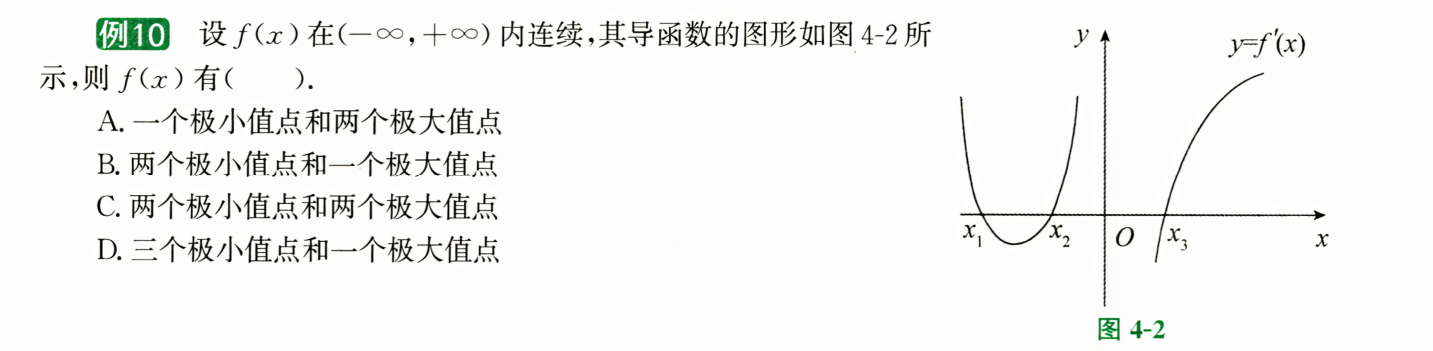
\includegraphics[width=390bp,height=135bp,keepaspectratio]{lilin-figures/第208页.png}

\vfill

\Solution

图中画的是 $f'$，它的正负决定原函数的升降。从左向右读图，$f'$ 在 $x_1$ 由正变负，所以 $f$ 在 $x_1$ 由增变减，有极大值。在 $x_2$ 由负变正，有极小值。

还要检查 $x=0$。此点的 $f'$ 虽然没有给出，但左侧导数为正、右侧导数为负，且题设保证 $f$ 连续。因此 $f$ 在零点由增变减，零点也是极大值点。最后在 $x_3$，$f'$ 由负变正，又产生一个极小值点。

合计两个极小值点 $x_2,x_3$，两个极大值点 $x_1,0$，选 C。查极值时，导数不存在的连续接合点也需要检查。

\clearpage

% SOURCE line=1328 pdf_page=209 section=2.6

\Question{203}{第4章 · 例题第2组 · 例 1}

求曲线 $f(x)=(x-5)x^{\frac{2}{3}}$ 的凹凸区间与拐点.

\vfill

\Solution

对于负数，$x^{\frac23}$ 表示 $\sqrt[3]{x^2}$。在 $x\ne0$ 处连续求导，得 $f'(x)=\frac53x^{-\frac13}(x-2)$，$f''(x)=\frac{10(x+1)}{9x^{\frac43}}$。分母始终为正，所以二阶导数的符号完全由 $x+1$ 决定。

在 $(-\infty,-1)$，$f''<0$，图像向下弯曲。在 $(-1,0)$ 和 $(0,+\infty)$，$f''>0$，图像向上弯曲。$x=-1$ 两侧凹凸改变，且曲线连续，代入得拐点 $(-1,-6)$。

$x=0$ 处导数不存在，需另外检查两侧凹凸。两侧二阶导数都为正，所以凹凸没有改变，零点不是拐点。凹凸区间也须在该尖点处分开。

\clearpage

% SOURCE line=1332 pdf_page=210 section=2.6

\Question{204}{第4章 · 例题第2组 · 例 2}

设 $f(x)$ 在 x=0 处有二阶连续导数，且 $f(0)=f'(0)=0, f''(0)\neq0$ ，证明：$(0,F(0))$ 是曲线 $F(x)=(1-\mathrm{e}^{2x})f(x)$ 的拐点.

\vfill

\Solution

拐点要检查二阶导数在两侧是否变号。设 $a=f''(0)\ne0$，由 $f(0)=f'(0)=0$，有 $f(x)=\frac12ax^2+o(x^2)$、$f'(x)=ax+o(x)$、$f''(x)=a+o(1)$。

对 $F$ 用乘积法则求两次导数，得到
\[
F''(x)=(1-\mathrm e^{2x})f''(x)-4\mathrm e^{2x}f'(x)-4\mathrm e^{2x}f(x).
\]
由于 $1-\mathrm e^{2x}=-2x+o(x)$，代入各项后得到 $F''(x)=-6ax+o(x)$。于是 $\frac{F''(x)}x\to-6a\ne0$，在零点两侧 $F''$ 的符号相反。$F$ 连续且 $F(0)=0$，故 $(0,0)$ 是拐点。

\clearpage

% SOURCE line=1336 pdf_page=211 section=2.6

\Question{205}{第4章 · 例题第2组 · 例 3}

设在定义域内 $f(x)$ 二阶可导, $g(x) = f(0)(1 - x) + f(1)x$, 则在 $[0,1]$ 上().

\textbf{A.} 当 $f'(x) \geqslant 0$ 时, $f(x) \geqslant g(x)$

\textbf{B.} 当 $f'(x) \geqslant 0$ 时, $f(x) \leqslant g(x)$

\textbf{C.} 当 $f''(x) \geqslant 0$ 时, $f(x) \geqslant g(x)$

\textbf{D.} 当 $f''(x) \geqslant 0$ 时, $f(x) \leqslant g(x)$

\vfill

\Solution

$g(x)$ 是连接 $(0,f(0))$ 与 $(1,f(1))$ 的直线。要比较曲线与这条弦，取任意 $0<x<1$，分别在 $[0,x]$ 和 $[x,1]$ 使用 Lagrange 中值定理，得
\[
\frac{f(x)-f(0)}x=f'(u),\qquad \frac{f(1)-f(x)}{1-x}=f'(v),\quad 0<u<x<v<1.
\]
若 $f''\geq0$，则 $f'$ 单调不减，所以第一个分式不超过第二个。乘以正数 $x(1-x)$ 并移项，得到 $f(x)\leq(1-x)f(0)+xf(1)=g(x)$。两个端点取等，故选 D。

只给 $f'\geq0$ 无法确定曲线位于弦的哪一侧。例如 $x^2$ 位于弦下方，$2x-x^2$ 位于弦上方，均在 $[0,1]$ 递增。

\clearpage

% SOURCE line=1348 pdf_page=212 section=2.6

\Question{206}{第4章 · 例题第2组 · 例 4}

设 $f(x)$ 有二阶连续导数, $L_{1}, L_{2}, L_{3}$ (见图4-6) 分别为曲线( ).

\textbf{A.} $y = f(x), y = f'(x), y = f''(x)$

\textbf{B.} $y = f(x), y = f''(x), y = f'(x)$

\textbf{C.} $y = f''(x), y = f'(x), y = f(x)$

\textbf{D.} $y = f'(x), y = f(x), y = f''(x)$ 图4-6

\par\smallskip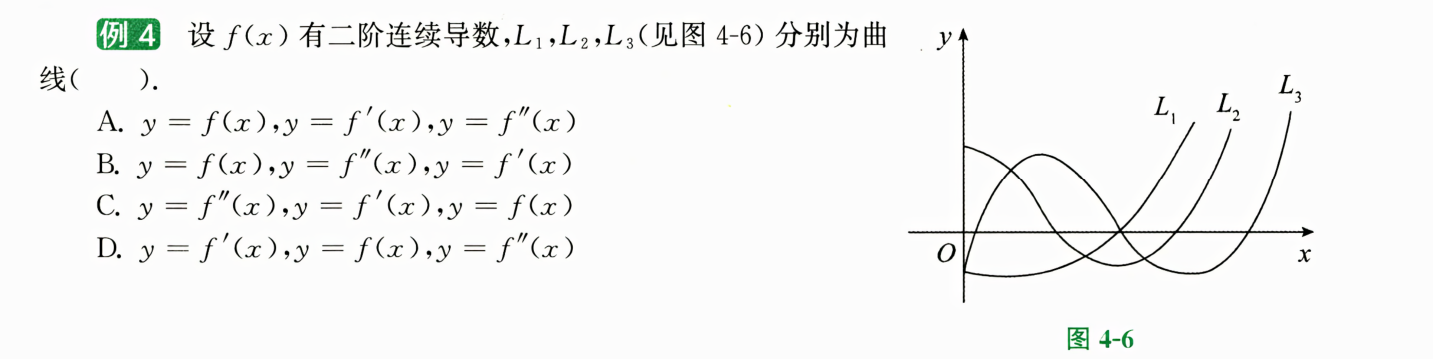
\includegraphics[width=390bp,height=135bp,keepaspectratio]{lilin-figures/第212页.png}

\vfill

\Solution

判断两条曲线谁是谁的导数，可以对照“函数的极值点对应导函数的零点”。先看 $L_2$，它先下降、到最低点后再上升。恰在它的最低点对应横坐标处，$L_1$ 从负值穿过横轴变成正值，所以 $L_1$ 是 $L_2$ 的导函数。

再看 $L_3$，它先升、后降、再升，依次有一个极大值和一个极小值。这两点分别对应 $L_2$ 从正到负、从负到正穿过横轴的位置。因此 $L_2$ 是 $L_3$ 的导函数。

导数关系串起来为 $L_3\to L_2\to L_1$，所以 $L_1$ 对应 $f''$、$L_2$ 对应 $f'$、$L_3$ 对应 $f$，选 C。

\clearpage

% SOURCE line=1384 pdf_page=216 section=2.6

\Question{207}{第4章 · 例题第2组 · 例 8}

讨论方程 $2x^{3}-9x^{2}+12x+k=0$ 不同实根的个数.

\vfill

\Solution

把左边记作 $H(x)$。三次函数在负无穷趋于负无穷，在正无穷趋于正无穷。求导得 $H'(x)=6(x-1)(x-2)$，所以先增、后减、再增，局部最高点在 $1$，最低点在 $2$。

算出 $H(1)=k+5$、$H(2)=k+4$。若最高点在横轴上方、最低点在横轴下方，三个单调区间各穿轴一次，所以 $-5<k<-4$ 时有三个不同实根。

$k=-5$ 或 $k=-4$ 时，某个极值点恰在横轴上，产生一个重根，另有一个不同实根，合计两个。其余情况下两个极值都在横轴同侧，只有最左段或最右段穿轴，合计一个实根。

\clearpage

% SOURCE line=1388 pdf_page=217 section=2.6

\Question{208}{第4章 · 例题第2组 · 例 9}

求方程 $k \arctan x = x$ 不同实根的个数，其中 k 为参数.

\vfill

\Solution

令 $H(x)=k\arctan x-x$。函数为奇函数，$x=0$ 总是一个根，所以只需研究正半轴。其导数为 $H'(x)=\frac{k}{1+x^2}-1$。

若 $k\leq1$，对 $x>0$ 总有 $H'(x)<0$。从 $H(0)=0$ 开始严格下降，因此正半轴无根，利用奇性，负半轴也无根，只有一个根 $0$。

若 $k>1$，导数在 $0<x<\sqrt{k-1}$ 为正，在 $x>\sqrt{k-1}$ 为负。函数从零先升至正的最大值，再严格下降到负无穷。由连续性与严格单调性，下降段恰有一个正根，其相反数是唯一负根。加上零点，共三个不同实根。

\clearpage

% SOURCE line=1392 pdf_page=218 section=2.6

\Question{209}{第4章 · 例题第2组 · 例 10}

设方程 $ax+\frac{1}{x^{2}}-1=0$ 在 $(0,+\infty)$ 内有两个不同实根，求 a 的取值范围.

\vfill

\Solution

因为 $x>0$，将方程解出参数 $a$，得到 $a=H(x)=\frac1x-\frac1{x^3}$。现在问题变成水平线 $y=a$ 与这条曲线有几个交点。

求导得 $H'(x)=\frac{3-x^2}{x^4}$。所以 $H$ 在 $(0,\sqrt3)$ 递增，在 $(\sqrt3,+\infty)$ 递减。左端趋于负无穷，右端从正侧趋于 $0$，而最大值为 $H(\sqrt3)=\frac{2}{3\sqrt3}$。

要让递增段和递减段各与水平线交一次，水平线必须严格位于 $0$ 与最大值之间。因此 $0<a<\frac{2}{3\sqrt3}$。取等于最大值时仅有切触点，取 $a=0$ 时右侧极限没有实际达到，均只有一个根。

\clearpage

% SOURCE line=1396 pdf_page=219 section=2.6

\Question{210}{第4章 · 例题第2组 · 例 11}

求曲线 $y=\frac{1}{x}+\ln(1+e^{x})$ 的渐近线方程.

\vfill

\Solution

先查定义域的有限断点 $x=0$。对数项趋于 $\ln2$，而 $\frac1x$ 无界，所以 $x=0$ 是竖直渐近线。

当 $x\to-\infty$，$\frac1x\to0$ 且 $\ln(1+\mathrm e^x)\to0$，因此 $y=0$ 是这一端的水平渐近线。

当 $x\to+\infty$，从对数中提出 $\mathrm e^x$，得 $\ln(1+\mathrm e^x)=x+\ln(1+\mathrm e^{-x})$，从而 $y-x=\frac1x+\ln(1+\mathrm e^{-x})\to0$。所以 $y=x$ 是这一端的斜渐近线。共得到三条渐近线。

\clearpage

% SOURCE line=1402 pdf_page=220 section=2.6

\Question{211}{第4章 · 选择题 · 第 1 题}

方程 $\left|x\right|^{\frac{1}{4}}+\left|x\right|^{\frac{1}{2}}=\cos x$ 不同实根的个数为( )。

\textbf{A.} 无实根

\textbf{B.} 有且只有一个实根

\textbf{C.} 有且只有两个实根

\textbf{D.} 无法确定

\vfill

\Solution

原方程两边都是偶函数，正根与负根成对出现，先看 $x\geq0$。当 $x\geq1$ 时，左边至少为 $2$，右边至多为 $1$，所以无解。

在 $[0,1]$，令 $H(x)=x^{\frac14}+x^{\frac12}-\cos x$。端点值 $H(0)=-1<0$，$H(1)=2-\cos1>0$，连续性保证至少有一个根。对 $0<x<1$，有 $H'(x)=\frac1{4x^{\frac34}}+\frac1{2\sqrt{x}}+\sin x>0$，所以函数严格递增，只能有一个根。

该根不等于零，取它的相反数又得到唯一负根。故共两个不同实根，选 C。

\clearpage

% SOURCE line=1414 pdf_page=221 section=2.6

\Question{212}{第4章 · 选择题 · 第 2 题}

设 $f(x)$ 在 $(-\infty, +\infty)$ 内连续，其导函数 $y = f'(x)$ 如图 4-10 所示，则（ ）。

\textbf{A.} $f(x)$ 有两个极值点，$y = f(x)$ 有两个拐点

\textbf{B.} $f(x)$ 有两个极值点，$y = f(x)$ 有三个拐点

\textbf{C.} $f(x)$ 有三个极值点，$y = f(x)$ 有一个拐点

\textbf{D.} $f(x)$ 有三个极值点，$y = f(x)$ 有两个拐点

\par\smallskip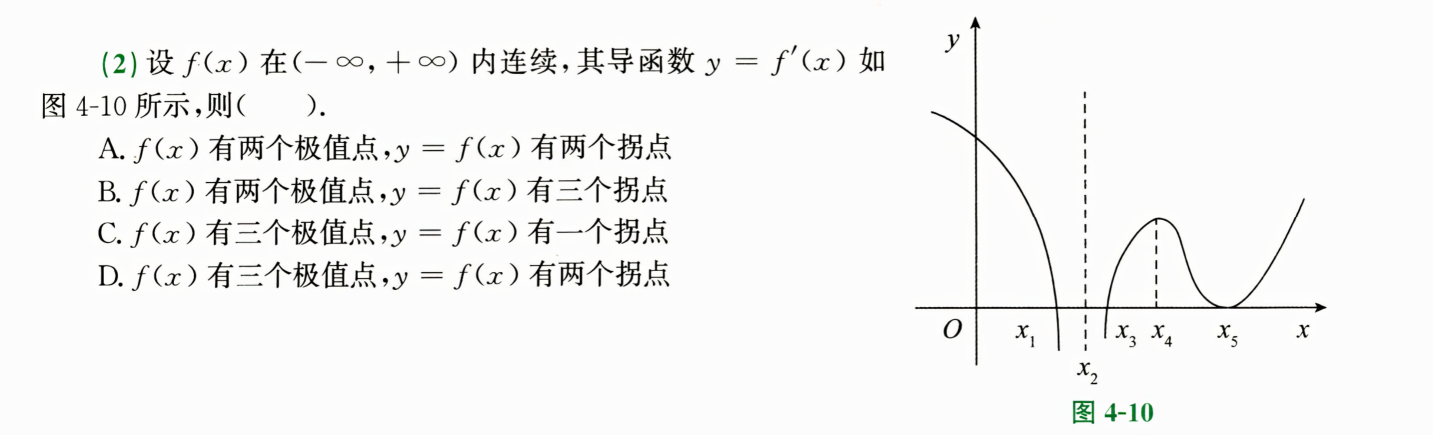
\includegraphics[width=390bp,height=135bp,keepaspectratio]{lilin-figures/第221页.png}

\vfill

\Solution

先根据 $f'$ 的正负数极值点。在 $x_1$，导数由正变负，原函数有极大值。在 $x_3$，导数由负变正，有极小值。$x_2$ 左右导数都为负，$x_5$ 左右导数都为正，这两点不产生极值。因此极值点共有两个。

再根据 $f'$ 的升降找拐点。$f'$ 下降时 $f''<0$，上升时 $f''>0$。图中 $f'$ 在 $x_2$ 由下降转为上升，在 $x_4$ 由上升转为下降，在 $x_5$ 又由下降转为上升，因此这三处凹凸改变。题设保证 $f$ 连续，即使 $x_2$ 处没有导数，仍能成为拐点。

合计两个极值点、三个拐点，选 B。

\clearpage

% SOURCE line=1428 pdf_page=222 section=2.6

\Question{213}{第4章 · 选择题 · 第 3 题}

曲线 $y=\frac{x^{2}+x}{x^{2}-1}$ 的渐近线的条数为( ).

\textbf{A.} 0

\textbf{B.} 1

\textbf{C.} 2

\textbf{D.} 3

\vfill

\Solution

先约分以分清真正的无穷间断点和可去间断点。除 $x=\pm1$ 外，$y=\frac{x(x+1)}{(x-1)(x+1)}=\frac{x}{x-1}=1+\frac1{x-1}$。

在 $x=1$ 附近，$\frac1{x-1}$ 无界，因此 $x=1$ 是竖直渐近线。在 $x=-1$ 附近，约分后的式子趋于 $\frac12$，原曲线只少了一个点，不产生渐近线。两端无穷远处 $\frac1{x-1}\to0$，所以水平渐近线为 $y=1$。共两条，选 C。

\clearpage

% SOURCE line=1442 pdf_page=223 section=2.6

\Question{214}{第4章 · 解答题 · 第 1 题}

求 $y = x + \frac{x}{x^{2}-1}$ 的单调区间、凹凸区间、极值和拐点.

\vfill

\Solution

定义域为 $x\ne\pm1$。先求一阶导数并通分，得 $y'=\frac{x^2(x^2-3)}{(x^2-1)^2}$。分母正，$x^2$ 非负，所以符号由 $x^2-3$ 决定。

递增区间为 $(-\infty,-\sqrt3)$、$(\sqrt3,+\infty)$。递减区间为 $(-\sqrt3,-1)$、$(-1,1)$、$(1,\sqrt3)$。其中 $x=0$ 仅使导数瞬间等于零，左右同为递减。极大值在 $x=-\sqrt3$，为 $-\frac{3\sqrt3}{2}$；极小值在 $x=\sqrt3$，为 $\frac{3\sqrt3}{2}$。

二阶导数为 $y''=\frac{2x(x^2+3)}{(x^2-1)^3}$。在 $(-\infty,-1)$、$(0,1)$ 为负，图像向下弯曲；在 $(-1,0)$、$(1,+\infty)$ 为正，图像向上弯曲。零点两侧凹凸改变，拐点为 $(0,0)$。$\pm1$ 不在定义域内，不能作拐点。

\clearpage

% SOURCE line=1446 pdf_page=224 section=2.6

\Question{215}{第4章 · 解答题 · 第 2 题}

证明: 不等式 $\ln\frac{b}{a}>\frac{2(b-a)}{b+a}$ (0<a<b).

\vfill

\Solution

先令 $t=\frac ba>1$，把含两个参数的不等式化成只含一个变量的 $\ln t>\frac{2(t-1)}{t+1}$。比较两个表达式时，可以研究它们的差。

设 $H(t)=\ln t-\frac{2(t-1)}{t+1}$。显然 $H(1)=0$，而
\[
H'(t)=\frac1t-\frac4{(t+1)^2}=\frac{(t-1)^2}{t(t+1)^2}>0\quad(t>1).
\]
所以从 $1$ 往右，$H$ 严格增加，$H(t)>H(1)=0$。将 $t=\frac ba$ 代回，即得到题目中的严格不等式。

\clearpage

% SOURCE line=1450 pdf_page=225 section=2.6

\Question{216}{第4章 · 解答题 · 第 3 题}

设 $y = f(x) = \left\{ \begin{aligned} & \sqrt[x]{x}, & x > 0, \\ & 0, & x = 0, \end{aligned} \right.$ 讨论 $f(x)$ 的连续性，并求 $f(x)$ 的单调区间、极值与渐近线.

\vfill

\Solution

对 $x>0$ 写成 $f(x)=\mathrm e^{\frac{\ln x}{x}}$。初等函数在正半轴连续。在 $x\to0^+$ 时，$\frac{\ln x}{x}\to-\infty$，故 $f(x)\to0=f(0)$，所以在定义域 $[0,+\infty)$ 上处处连续，端点按右连续理解。

对正半轴用链式法则，得 $f'(x)=x^{\frac1x}\frac{1-\ln x}{x^2}$。除 $1-\ln x$ 外其余因子均为正，故在 $(0,\mathrm e)$ 递增，在 $(\mathrm e,+\infty)$ 递减。$x=\mathrm e$ 处取得极大值，也是最大值 $\mathrm e^{\frac1{\mathrm e}}$；内部没有极小值，端点 $x=0$ 取得全域最小值 $0$。

无穷远处 $\frac{\ln x}{x}\to0$，所以 $f(x)\to1$，渐近线为 $y=1$。有限端点的函数值有限，没有竖直渐近线。

\clearpage

% SOURCE line=1454 pdf_page=226 section=2.6

\Question{217}{第4章 · 解答题 · 第 4 题}

比较$\pi^{e}$与$e^{\pi}$的大小.

\vfill

\Solution

两个幂的底数和指数不同，先取自然对数，比较 $\mathrm e\ln\pi$ 与 $\pi$，再除以正数 $\mathrm e\pi$，就变成比较 $\frac{\ln\pi}{\pi}$ 与 $\frac1{\mathrm e}$。

令 $H(x)=\frac{\ln x}{x}$，其导数为 $H'(x)=\frac{1-\ln x}{x^2}$。当 $x>\mathrm e$ 时导数为负，所以 $H$ 在这一段严格递减。因为 $\pi>\mathrm e$，有 $H(\pi)<H(\mathrm e)=\frac1{\mathrm e}$。乘回正数并取指数，得到 $\pi^{\mathrm e}<\mathrm e^\pi$。

\clearpage

% SOURCE line=1458 pdf_page=227 section=2.6

\Question{218}{第4章 · 解答题 · 第 5 题}

设当 x > 0 时，方程 $\ln a = \frac{\ln x}{x}$ 有实根，求 a 的取值范围.

\vfill

\Solution

左边 $\ln a$ 要有定义，先要求 $a>0$。再研究右边 $H(x)=\frac{\ln x}{x}$ 在正半轴能取到哪些值。其导数为 $H'(x)=\frac{1-\ln x}{x^2}$，在 $(0,\mathrm e)$ 为正，在 $(\mathrm e,+\infty)$ 为负，所以最大值在 $x=\mathrm e$ 取得，为 $\frac1{\mathrm e}$。

同时 $H(x)$ 在 $x\to0^+$ 时趋于负无穷，且在 $(0,\mathrm e]$ 连续递增，因此值域正好是 $(-\infty,\frac1{\mathrm e}]$。方程有解当且仅当 $\ln a\leq\frac1{\mathrm e}$，即 $0<a\leq\mathrm e^{\frac1{\mathrm e}}$。

\clearpage

% SOURCE line=2151 pdf_page=345 section=2.6

\Question{219}{第7章 · 例题第1组 · 例 2}

设某商品的需求函数为 $Q = 100 - 5P$，其中价格 $P \in (0, 20)$，Q 为需求量。

(1) 求需求量对价格的弹性 $E_{d}(E_{d}>0)$;

(2) 证明：$\frac{dR}{dP}=Q(1-E_{d})$（R 表示收益），并用弹性 $E_{d}$ 说明当价格在何范围内时，降价反而使收益增加.

\vfill

\Solution

需求弹性 $E_d=-\frac{P}{Q}\frac{\mathrm dQ}{\mathrm dP}$，描述价格上涨百分之一时需求量下降百分之几。负号使通常递减的需求对应正弹性。因为 $Q=100-5P$，$Q'=-5$，所以 $E_d=\frac{5P}{100-5P}=\frac{P}{20-P}$。

销售收入等于单价乘销量，$R=PQ$。用乘积法则得 $R'=Q+PQ'=Q(1-E_d)$。当 $E_d>1$ 时，$R'<0$，所以降低价格会增加收入。解 $\frac{P}{20-P}>1$，分母在已知区间为正，得到 $10<P<20$。

也可直接核实 $R(P)=100P-5P^2$、$R'(P)=100-10P$，在上述区间确为负。

\clearpage

% SOURCE line=2167 pdf_page=347 section=2.6

\Question{220}{第7章 · 例题第1组 · 例 4}

为实现利润最大化，厂商需要对某商品确定其定价模型。设 Q 为该商品的需求量，P 为价格，MC 为边际成本，$\eta$ 为需求弹性（$\eta>0$）。

(1) 证明: 定价模型为 $P = \frac{MC}{1 - \frac{1}{\eta}}$;

(2) 若该商品的成本函数为 $C(Q) = 1600 + Q^{2}$，需求函数为 Q = 40 - P，试求由(1)中定价模型确定的此商品价格.

\vfill

\Solution

设价格可写成销量的函数 $P=P(Q)$，利润为 $\Pi(Q)=P(Q)Q-C(Q)$。边际成本指 $MC=C'(Q)$，需求弹性为 $\eta=-\frac{P}{Q}\frac{\mathrm dQ}{\mathrm dP}$。因此 $P'(Q)=-\frac{P}{\eta Q}$。

内点利润最大时，导数必须为零：$\Pi'=P+QP'-MC=P(1-\frac1\eta)-MC=0$。当 $\eta\ne1$ 时，解得定价模型 $P=\frac{MC}{1-\frac1\eta}$。这给出最优内点的必要条件，具体题中还需检查确为最大值。

（2）由 $Q=40-P$ 得 $P=40-Q$，故 $\Pi=(40-Q)Q-(1600+Q^2)=40Q-2Q^2-1600$。其导数为 $40-4Q$，二阶导数为 $-4<0$，所以 $Q=10$ 时利润最大，价格为 $P=30$。此时 $MC=20$、$\eta=\frac PQ=3$，代入模型也得到 $30$。

\clearpage

% SOURCE line=2189 pdf_page=351 section=2.6

\Question{221}{第7章 · 解答题 · 第 1 题}

设某产品在日产量为 x（件）时，其总成本函数为 $C(x)=100+18x-40\sqrt{x}$（百元），求使平均成本为最小的日产量.

\vfill

\Solution

平均成本是每件分摊的总成本，故目标函数为 $A(x)=\frac{C(x)}x=\frac{100}{x}+18-\frac{40}{\sqrt{x}}$，其中 $x>0$。求导并把分母统一成正数 $x^2$，得到
\[
A'(x)=-\frac{100}{x^2}+\frac{20}{x^{\frac32}}=\frac{20(\sqrt{x}-5)}{x^2}.
\]
当 $0<x<25$ 时导数为负，$x>25$ 时为正，所以平均成本先减后增，在 $x=25$ 取得全域最小值。日产量应为 $25$ 件。代入可查平均成本为 $\frac{100}{25}+18-\frac{40}{5}=14$ 百元每件。

\clearpage

% SOURCE line=2209 pdf_page=356 section=2.6

\Question{222}{第7章 · 解答题 · 第 6 题}

设某酒厂有一批新酿好酒，若现在 $(t=0)$ 出售，总收入为 $R_{0}$，若窑陈起来，按陈酒价格出售，t 年末总收入为 $R=R_{0}e^{\frac{2}{5}\sqrt{t}}$，现设银行年利率为 r，以连续复利计算，求窑陈多少年售出可使总收入现值最大，并求 r=0.06 时，t 的值.

\vfill

\Solution

连续复利的折现因子是 $\mathrm e^{-rt}$。因此 $t$ 年后的收入折算到现在，现值为 $V(t)=R_0\mathrm e^{\frac25\sqrt t-rt}$，$t\geq0$。指数函数严格递增，只需使指数 $H(t)=\frac25\sqrt t-rt$ 最大。

在通常的正利率 $r>0$ 下，$H'(t)=\frac1{5\sqrt t}-r$。它在 $t<\frac1{25r^2}$ 时为正，在更大时为负，因此最优窖陈时间为 $t_*=\frac1{25r^2}$ 年，最大现值为 $R_0\mathrm e^{\frac1{25r}}$。

当 $r=0.06=\frac3{50}$，$t_*=\frac{100}{9}$ 年，约 $11.11$ 年。若 $r\leq0$，指数始终上升，没有有限的最优售出时间。

\clearpage

\clearpage\pdfbookmark[0]{第3章 一元函数积分学及其应用}{c3}

\SectionHeading{3.1}{定积分的概念、存在条件与性质}

% SOURCE line=245 pdf_page=40 section=3.1

\Question{223}{第1章 · 例题第3组 · 例 4}

设 $f(x)$ 在 $[0,1]$ 上连续，且 $f(x) > 0$，求极限 $\lim_{n \to \infty} \sqrt[n]{f\left(\frac{1}{n}\right) f\left(\frac{2}{n}\right) \cdots f\left(\frac{n-1}{n}\right) f(1)}$.

\vfill

\Solution

开 $n$ 次方根的连乘积是几何平均。取对数能把连乘积变成求和，把根号变成系数 $\frac1n$。令原数列为 $A_n$，则
\[
\ln A_n=\sum_{k=1}^n \ln f\left(\frac{k}{n}\right)\frac1n.
\]
由于 $f$ 在闭区间上连续且为正，$\ln f$ 也连续。把 $[0,1]$ 分成 $n$ 个等长小区间，每段长 $\frac1n$，取每一段右端点 $\frac kn$，上式正是 Riemann 和。它趋于 $\int_0^1\ln f(t)\,\mathrm dt$。再取指数得 $\exp(\int_0^1\ln f(t)\,\mathrm dt)$。若 $f\equiv c>0$，该式给出 $c$，和原数列一致。

\clearpage

% SOURCE line=250 pdf_page=41 section=3.1

\Question{224}{第1章 · 例题第3组 · 例 5}

求$\lim_{n\to\infty}\left(\frac{\sin\frac{\pi}{n}}{n+1}+\frac{\sin\frac{2\pi}{n}}{n+\frac{1}{2}}+\cdots+\frac{\sin\frac{n\pi}{n}}{n+\frac{1}{n}}\right)$.

\vfill

\Solution

分子出现 $\sin(\frac{k\pi}n)$，说明应该凑成等分区间上的积分和。分母 $n+\frac1k$ 跟 $n$ 很接近，先严格估计换成 $n$ 的误差：
\[
0\le \frac1n-\frac1{n+\frac1k}
=\frac{\frac1k}{n(n+\frac1k)}\le\frac1{n^2}.
\]
正弦绝对值至多为 $1$，所以 $n$ 项总误差至多为 $\frac1n\to0$。替换后的和是 $\sum_{k=1}^n \sin(\frac{k\pi}n)\frac1n$，按 $[0,1]$ 右端点取值，趋于 $\int_0^1\sin(\pi t)\,\mathrm dt=\frac2\pi$。原极限相同。

\clearpage

% SOURCE line=498 pdf_page=75 section=3.1

\Question{225}{第1章 · 解答题 · 第 4 题}

求下列极限： （I）$\lim_{n\to\infty}\left(\frac{1}{n^2+n+1}+\frac{2}{n^2+n+2}+\cdots+\frac{n}{n^2+n+n}\right)$;

（II）$\lim_{n\to\infty}\frac{1}{n}\left(\frac{\sqrt{n^2-1^2}}{n}+\frac{\sqrt{n^2-2^2}}{n}+\cdots+\frac{\sqrt{n^2-n^2}}{n}\right)$.

\vfill

\Solution

（I）对 $1\le k\le n$，分母 $n^2+n+k$ 介于 $n^2+n$ 和 $n^2+2n$ 之间。所以
\[
\frac{n(n+1)}{2(n^2+2n)}
\le\sum_{k=1}^n\frac{k}{n^2+n+k}
\le\frac{n(n+1)}{2(n^2+n)}.
\]
两端都趋于 $\frac12$，由夹逼准则，第一问为 $\frac12$。

（II）把根式提出 $n$，写成 $\sum_{k=1}^n\frac1n\sqrt{1-(\frac kn)^2}$。这是 $[0,1]$ 等分后取右端点的 Riemann 和，所以极限为 $\int_0^1\sqrt{1-t^2}\,\mathrm dt$。曲线 $y=\sqrt{1-t^2}$ 是单位圆的上半部，在 $0\le t\le1$ 下方的面积是四分之一圆，故第二问为 $\frac\pi4$。

\clearpage

% SOURCE line=1636 pdf_page=255 section=3.1

\Question{226}{第6章 · 例题第1组 · 例 1}

证明:不等式$\frac{1}{2}<\int_{\frac{\pi}{4}}^{\frac{\pi}{2}}\frac{\sin x}{x}dx<\frac{\sqrt{2}}{2}$.

\vfill

\Solution

积分区间长为 $\frac\pi4$。如果能找出被积函数的最大、最小值，再乘区间长度，就能得到上下界。设 $h(x)=\frac{\sin x}{x}$，求导得
\[
h'(x)=\frac{x\cos x-\sin x}{x^2}.
\]
令 $u(x)=x\cos x-\sin x$，有 $u(0)=0$ 且 $u'(x)=-x\sin x<0$，因此 $h'<0$。两个端点值分别为 $\frac{2\sqrt2}{\pi}$ 与 $\frac2\pi$。内部各点严格介于二者之间，乘区间长度 $\frac\pi4$ 即得 $\frac12<I<\frac{\sqrt2}{2}$。

\clearpage

% SOURCE line=1746 pdf_page=280 section=3.1

\Question{227}{第6章 · 例题第2组 · 例 8}

求$\lim_{t\to0^{+}}\frac{1}{1-\mathrm{e}^{-t^{2}}}\int_{0}^{t}\mathrm{d}x\int_{t}^{x}\mathrm{e}^{-(x-y)^{2}}\mathrm{d}y$.

\vfill

\Solution

先留意内积分下限 $t$ 大于上限 $x$，因此带负号。对 $0\le x\le y\le t$，有 $0\le(y-x)^2\le t^2$，从而 $e^{-t^2}\le e^{-(x-y)^2}\le1$。翻转内积分方向后，再乘回负号得
\[
-\frac{t^2}{2}\le
\int_0^t dx\int_t^x e^{-(x-y)^2}\,dy
\le -e^{-t^2}\frac{t^2}{2},
\]
这里 $\int_0^t(t-x)\,dx=\frac{t^2}2$。分母 $1-e^{-t^2}>0$ 且与 $t^2$ 等价，两个端点除以分母都趋于 $-\frac12$。由夹逼准则即得答案。只用一元积分的逐次估计。

\clearpage

% SOURCE line=1752 pdf_page=281 section=3.1

\Question{228}{第6章 · 例题第3组 · 例 1}

设 $f(x)$ 在 $[0,+\infty)$ 上连续且单调减少，证明：当 0 < a < b 时，有 $a \int_{0}^{b} f(x) \, dx \leqslant b \int_{0}^{a} f(x) \, dx$.

\vfill

\Solution

把要证的式子移项并拆开 $[0,b]$，目标等价于
\[
(b-a)\int_0^a f(x)\,dx \ \ge\ a\int_a^b f(x)\,dx .
\]
左右各自除以 $a(b-a)>0$ 后，恰好比较前后两个区间的平均值。由单调减少，前半段每个函数值至少为 $f(a)$，所以左边积分至少为 $a f(a)$。后半段每个函数值至多为 $f(a)$，所以右边积分至多为 $(b-a)f(a)$。分别乘回正的区间长度就得到不等式。这一思路对负值函数同样成立。

\clearpage

% SOURCE line=1776 pdf_page=285 section=3.1

\Question{229}{第6章 · 例题第3组 · 例 5}

设 $I_{k}=\int_{0}^{k\pi}e^{x^{2}}\sin x\,dx$ ($k=1,2,3$)，则（）.

\textbf{A.} $I_{1}<I_{2}<I_{3}$

\textbf{B.} $I_{3}<I_{2}<I_{1}$

\textbf{C.} $I_{2}<I_{3}<I_{1}$

\textbf{D.} $I_{2}<I_{1}<I_{3}$

\vfill

\Solution

正弦函数每隔 $\pi$ 变号。将三段都平移到 $[0,\pi]$，设
\[
J_k=\int_0^\pi e^{(x+k\pi)^2}\sin x\,dx,\qquad k=0,1,2 .
\]
因 $x$ 在正半轴且 $\sin x$ 在内部为正，随 $k$ 增大被积式严格增大，所以 $0<J_0<J_1<J_2$。原积分依次为 $I_1=J_0$、$I_2=J_0-J_1$、$I_3=J_0-J_1+J_2$。这样 $I_2<I_1$，且 $I_3-I_1=J_2-J_1>0$，即 $I_2<I_1<I_3$，选 \textbf{D}。

\clearpage

% SOURCE line=1788 pdf_page=286 section=3.1

\Question{230}{第6章 · 例题第3组 · 例 6}

设 $f(x)$ 在 $[0,1]$ 上有连续导数，且 $f(0)=f(1)=0$，证明：$\left|\int_{0}^{1}f(x)dx\right|\leqslant\frac{M}{4}$，其中 $M=\max_{0\leqslant x\leqslant1}\left\{\left|f'(x)\right|\right\}$.

\vfill

\Solution

两个端点的函数值都是零。$|f'|\le M$ 的意思是，离哪个端点较近，就能从哪个端点得到更好的界。对 $0,x$ 用 Lagrange 中值定理得 $|f(x)|\le Mx$，对 $x,1$ 使用则得 $|f(x)|\le M(1-x)$。取较小者，再积分：
\[
\left|\int_0^1 f(x)\,dx\right|
\le M\left(\int_0^{\frac12}x\,dx+\int_{\frac12}^1(1-x)\,dx\right)
=M\left(\frac18+\frac18\right)=\frac M4 .
\]
只使用一个端点时上界为 $\frac M2$，取最近端点正好让估计更紧。

\clearpage

% SOURCE line=1792 pdf_page=287 section=3.1

\Question{231}{第6章 · 例题第3组 · 例 7}

设 $s(x)=\int_{0}^{x}\left|\cos t\right|\mathrm{d}t.$

(1) 当 n 为正整数，且 $n\pi \leqslant x < (n+1)\pi$ 时，证明：$2n \leqslant s(x) < 2(n+1)$.

(2) 求 $\lim_{x \to +\infty} \frac{s(x)}{x}$.

\vfill

\Solution

(1) $|\cos t|$ 的周期为 $\pi$。一个周期内，把 $[\frac\pi2,\pi]$ 的负余弦取相反数，总积分为 $2$，故 $s(n\pi)=2n$。$s$ 随 $x$ 严格增加，因为任何非零长度区间里都有一段 $|\cos t|>0$。于是 $2n\le s(x)<2(n+1)$。

(2) 取 $n$ 为满足 $n\pi\le x<(n+1)\pi$ 的整数。把分子、分母分别用上述界估计，有
\[
\frac{2n}{(n+1)\pi}\le\frac{s(x)}x\le\frac{2(n+1)}{n\pi}.
\]
$x\to+\infty$ 时 $n\to+\infty$，两端都趋于 $\frac2\pi$，由夹逼准则得到该极限。

\clearpage

% SOURCE line=1820 pdf_page=291 section=3.1

\Question{232}{第6章 · 例题第3组 · 例 11}

设 $f(x)$ 在 $[0,\pi]$ 上连续，且 $\int_{0}^{\pi}f(x)dx=\int_{0}^{\pi}f(x)\cos xdx=0$，证明：在 $(0,\pi)$ 内至少存在两个不同的点 $\xi_{1},\xi_{2}$，使得 $f(\xi_{1})=f(\xi_{2})=0$。

\vfill

\Solution

若 $f$ 在内部处处为零，结论直接成立。否则，第一条积分为零迫使 $f$ 在内部既取正值也取负值。由连续性，至少有一个零点。假设只有一个零点 $\xi$，则 $f$ 在 $\xi$ 两侧符号相反，且每一侧都不变号。

为了与 $f$ 一同在 $\xi$ 换号，构造 $h(x)=\cos x-\cos\xi$。因余弦在 $(0,\pi)$ 严格递减，$h$ 左正右负。因此 $f(x)h(x)$ 在两侧同号且均非零，积分不可能为零。然而两条已知积分关系给出 $\int_0^\pi f(x)h(x)dx=0$，矛盾，所以至少有两个不同的内部零点。

\clearpage

% SOURCE line=1960 pdf_page=313 section=3.1

\Question{233}{第6章 · 选择题 · 第 1 题}

设 $M=\int_{0}^{\frac{\pi}{4}}\frac{\tan x}{x}dx$，$N=\int_{0}^{\frac{\pi}{4}}\frac{x}{\tan x}dx$，则( )。

\textbf{A.} M > N > 1

\textbf{B.} 1 > M > N

\textbf{C.} N > M > 1

\textbf{D.} 1 > N > M

\vfill

\Solution

在 $0<x\le\frac\pi4$，有 $\tan x>x$，所以逐点比较得到 $M>N$ 且 $N<\frac\pi4<1$。还需要判断 $M$ 与 $1$ 的关系。

设 $h(x)=\frac{\tan x}{x}$。其导数的符号等于 $x-\sin x\cos x$ 的符号。后者在 $0$ 为零，导数为 $1-\cos2x>0$，故 $h$ 严格增加，且 $h(\frac\pi4)=\frac4\pi$。于是
\[
M=\int_0^{\frac\pi4}h(x)\,dx
<\frac\pi4\cdot\frac4\pi=1 .
\]
综合得到 $1>M>N$，选 \textbf{B}。两个被积函数在 $0$ 都可按极限补成 $1$。

\clearpage

% SOURCE line=1984 pdf_page=315 section=3.1

\Question{234}{第6章 · 选择题 · 第 3 题}

设在 $[a, b]$ 上，$f(x) > 0$，$f'(x) < 0$，$f''(x) > 0$，记 $S_{1}=\int_{a}^{b}f(x)dx,\quad S_{2}=f(b)(b-a),\quad S_{3}=\frac{1}{2}[f(a)+f(b)](b-a),$ 则（）.

\textbf{A.} $S_{1}<S_{2}<S_{3}$

\textbf{B.} $S_{2}<S_{1}<S_{3}$

\textbf{C.} $S_{3}<S_{1}<S_{2}$

\textbf{D.} $S_{2}<S_{3}<S_{1}$

\vfill

\Solution

三个量分别是曲线下方的面积、以右端高度作出的矩形面积、以两端高度作出的梯形面积。因为 $f'<0$，内部 $x$ 都满足 $f(x)>f(b)$，积分得 $S_1>S_2$。

又因 $f''>0$，$f'$ 严格增加，曲线位于两个端点连成的弦下方。因此
\[
f(x)<\frac{b-x}{b-a}f(a)+\frac{x-a}{b-a}f(b),\qquad a<x<b .
\]
两边积分，右边两个线性权重的积分均为 $\frac{b-a}{2}$，得到 $S_1<S_3$。所以 $S_2<S_1<S_3$，选 \textbf{B}。

\clearpage

% SOURCE line=2012 pdf_page=317 section=3.1

\Question{235}{第6章 · 填空题 · 第 1 题}

$\lim_{n \to \infty} \sum_{i=1}^{n} \frac{e^{\frac{i}{n}}}{n + n e^{\frac{2i}{n}}} =$ \underline{\hspace{4em}}.

\vfill

\Solution

把每项提取 $\frac1n$，原和式变为 $\sum_{i=1}^n\frac1n\,\frac{e^{\frac in}}{1+e^{\frac{2i}n}}$。这对应把 $[0,1]$ 等分成 $n$ 份，每段长度为 $\frac1n$，取右端点 $\frac in$ 的 Riemann 和。被积函数连续，所以极限为
\[
\int_0^1\frac{e^x}{1+e^{2x}}dx.
\]
令 $u=e^x$，$du=e^x dx$，上下限变为 $1,e$，所得积分为 $\int_1^e\frac{du}{1+u^2}=\arctan e-\frac\pi4$。识别步长和取样点后，数列极限就变成定积分计算。

\clearpage

% SOURCE line=2047 pdf_page=325 section=3.1

\Question{236}{第6章 · 解答题 · 第 5 题}

求 $\lim_{n \to \infty} \sum_{i=1}^{n} \frac{1}{n + \frac{i^2 + 1}{n}}$.

\vfill

\Solution

每项提取 $\frac1n$ 后，原和为
\[
S_n=\frac1n\sum_{i=1}^n\frac1{1+(\frac in)^2+\frac1{n^2}}.
\]
先去掉随 $n$ 变化的 $\frac1{n^2}$，记 $T_n=\frac1n\sum_{i=1}^n\frac1{1+(\frac in)^2}$。两项分式作差，分母都至少为 $1$，所以 $0\le T_n-S_n\le\frac1{n^2}$，误差趋于零。$T_n$ 是连续函数 $\frac1{1+x^2}$ 在 $[0,1]$ 上的右端点 Riemann 和，因此 $T_n\to\int_0^1\frac{dx}{1+x^2}=\frac\pi4$。由误差估计，$S_n$ 的极限也为 $\frac\pi4$。

\clearpage

% SOURCE line=2073 pdf_page=331 section=3.1

\Question{237}{第6章 · 解答题 · 第 11 题}

设 $f(x)$ 在 $[a,b]$ 上有连续导数, $f(a)=0$ ，证明： $\frac{2}{(b-a)^{2}}\int_{a}^{b}\left|f(x)\right|\mathrm{d}x\leqslant M,\quad M=\max_{x\in\left[a,b\right]}\left|f'(x)\right|.$

\vfill

\Solution

条件给了导数的最大绝对值，先用 Lagrange 中值定理把它变成函数值的界。对每个 $x\in(a,b]$，存在 $\xi$ 在 $a,x$ 之间，使 $f(x)-f(a)=f'(\xi)(x-a)$。由 $f(a)=0$，得到 $|f(x)|\le M(x-a)$。

接着两边积分，
\[
\int_a^b|f(x)|dx\le M\int_a^b(x-a)dx=\frac M2(b-a)^2 .
\]
题设分母 $(b-a)^2$ 为正，将它除到左边并乘以 $2$ 就得到结论。这里使用绝对值后上界始终非负，允许 $f$ 在区间内变号。

\clearpage

% SOURCE line=2078 pdf_page=332 section=3.1

\Question{238}{第6章 · 解答题 · 第 12 题}

设 $f(x)$ 是 $[0,a]$ 上的正值函数，且 $f''(x) > 0$，$a > 0$，证明：$\int_{0}^{a}f(x)dx \geqslant af\left(\frac{a}{2}\right)$.

\vfill

\Solution

右边是「区间长度乘以中点处的函数值」。为了让中点自然出现，在 $c=\frac a2$ 处作切线。由 $f''>0$，$f'$ 严格增加，曲线位于这条切线上方。具体地，对 $x>c$，中值定理给出的斜率大于 $f'(c)$；对 $x<c$，斜率小于 $f'(c)$，但乘上负的 $x-c$ 后方向反转。因此两种情况都有
\[
f(x)\ge f(c)+f'(c)(x-c).
\]
积分后 $\int_0^a(x-c)dx=0$，切线的倾斜部分相消，留下 $\int_0^a f(x)dx\ge af(c)$，即所证。由于 $f''>0$，当 $x\ne c$ 实际为严格大于。

\clearpage

% SOURCE line=2082 pdf_page=333 section=3.1

\Question{239}{第6章 · 解答题 · 第 13 题}

设 $f''(x) > 0, x \in [a, b]$，证明： $f\left(\frac{a+b}{2}\right)\leqslant\frac{1}{b-a}\int_{a}^{b}f(x)dx$

\vfill

\Solution

设区间中点为 $c=\frac{a+b}{2}$。$f''>0$ 保证 $f'$ 严格增加。用中值定理可得曲线在中点的切线上方，
\[
f(x)\ge f(c)+f'(c)(x-c),\qquad a\le x\le b.
\]
理由是 $x>c$ 时，割线斜率至少为 $f'(c)$；$x<c$ 时割线斜率至多为 $f'(c)$，乘负的横坐标增量后又得到同一方向的不等式。两边积分，线性项关于中点奇对称，所以积分为零。得 $\int_a^b f(x)dx\ge(b-a)f(c)$。除以正数 $b-a$，便得题设结论。

\clearpage

\SectionHeading{3.2}{微积分基本公式与基本定理}

% SOURCE line=93 pdf_page=13 section=3.2

\Question{240}{第1章 · 例题第1组 · 例 12}

设 $f(x)$ 是连续函数, $F(x)=\int_{a}^{x}f(t)dt$, 则( ).

\textbf{A.} 当 $f(x)$ 是奇函数时，$F(x)$ 必是偶函数

\textbf{B.} 当 $f(x)$ 是偶函数时，$F(x)$ 必是奇函数

\textbf{C.} 当 $f(x)$ 是周期函数时，$F(x)$ 必是周期函数

\textbf{D.} 当 $f(x)$ 是单调增加函数时，$F(x)$ 必是单调增加函数

\vfill

\Solution

遇到下限 $a$，先把它移到对称中心 $0$。写成 $F(x)=G(x)-G(a)$，其中 $G(x)=\int_0^x f(t)\,\mathrm dt$。令 $t=-u$，得 $G(-x)=-\int_0^x f(-u)\,\mathrm du$。若 $f$ 为奇函数，则 $G(-x)=G(x)$，减常数仍为偶函数，因此 A 正确。

B 对任意 $a$ 不成立，例如 $f\equiv1,a=1$ 时 $F(x)=x-1$。同取 $f\equiv1$，其积分是斜率为 $1$ 的直线，故 C 也不成立。D 的关键是 $F'=f$ 的正负。取 $f(x)=x$，则 $F'(x)=x<0$ 在负半轴成立，所以 $F$ 在该处递减。选 \textbf{A}。

\clearpage

% SOURCE line=207 pdf_page=33 section=3.2

\Question{241}{第1章 · 例题第2组 · 例 19}

当 $x \to 0^{+}$ 时，将无穷小 $\alpha = \int_{0}^{x} \cos t^{2} \, dt, \beta = \int_{0}^{x^{2}} \arctan \sqrt{t} \, dt, \gamma = \int_{0}^{\sqrt{x}} \sin t^{3} \, dt$ 排序，使排在后面的是前一个的高阶无穷小，则正确的排列顺序是（ ）。

\textbf{A.} $\alpha,\gamma,\beta$

\textbf{B.} $\alpha,\beta,\gamma$

\textbf{C.} $\beta,\gamma,\alpha$

\textbf{D.} $\beta,\alpha,\gamma$

\vfill

\Solution

比较无穷小时先找各自的最低次幂。这里每个积分区间都缩到 $0$。如果被积函数与 $t^p$ 的比值趋于 $1$，那么在足够小的正区间上，它被 $(1-\varepsilon)t^p$ 和 $(1+\varepsilon)t^p$ 夹住。积分后可用同样的比值比较。

$\cos(t^2)\to1$，故 $\alpha\sim x$。$\arctan\sqrt t\sim\sqrt t$，故 $\beta\sim\int_0^{x^2}\sqrt t\,\mathrm dt=\frac23x^3$。$\sin(t^3)\sim t^3$，故 $\gamma\sim\int_0^{\sqrt x}t^3\,\mathrm dt=\frac14x^2$。

当 $x\to0^+$，二次项比一次项更快趋于零，三次项比二次项更快。排列为 $\alpha,\gamma,\beta$，选 \textbf{A}。

\clearpage

% SOURCE line=697 pdf_page=106 section=3.2

\Question{242}{第2章 · 例题第2组 · 例 7}

（数学三不要求）设 $y = y(x)$ 由 $\left\{\begin{array}{l}x = e^{-t}, \\ y = \int_{0}^{t} \ln(1 + u^{2}) du\end{array}\right.$ 确定，求 $\left.\frac{d^{2}y}{dx^{2}}\right|_{t=0}$.

\vfill

\Solution

先求关于参数 $t$ 的导数。变上限积分的导数等于把上限代入被积函数，所以 $y_t=\ln(1+t^2)$，而 $x_t=-\mathrm e^{-t}$。故一阶导数为 $y_x=-\mathrm e^t\ln(1+t^2)$。

二阶导数要求的是 $y_x$ 对 $x$ 的变化率。先对 $t$ 求导，再除以 $x_t$：
\[
y_{xx}=\frac{-\mathrm e^t[\ln(1+t^2)+\frac{2t}{1+t^2}]}{-\mathrm e^{-t}}=\mathrm e^{2t}\left[\ln(1+t^2)+\frac{2t}{1+t^2}\right].
\]
代入 $t=0$，两项都为零，结果为 $0$。

\clearpage

% SOURCE line=1152 pdf_page=176 section=3.2

\Question{243}{第3章 · 解答题 · 第 5 题}

设 $f(x)$ 在 $[0,1]$ 上连续，在 $(0,1)$ 内可导，且 $\int_{0}^{1}f(x)dx=0$，证明：存在一点 $\xi\in(0,1)$，使得 $\int_{0}^{\xi}f(x)dx=-\xi f(\xi)$.

\vfill

\Solution

把变上限积分记为 $A(x)=\int_0^xf(t)\,\mathrm dt$。由 $f$ 连续和微积分基本定理，$A'(x)=f(x)$。目标是 $A(\xi)+\xi A'(\xi)=0$，恰好是乘积 $xA(x)$ 的导数等于零。

令 $F(x)=xA(x)$。它在闭区间连续、内部可导，且 $F(0)=0$、$F(1)=\int_0^1 f=0$。因此 Rolle 定理给出内部一点 $\xi$ 使 $F'(\xi)=0$。用乘积法则得
\[
0=A(\xi)+\xi f(\xi),
\]
移项即 $\int_0^\xi f(x)\,\mathrm dx=-\xi f(\xi)$。辅助函数的选择直接来自要证明的等式左侧。

\clearpage

% SOURCE line=1156 pdf_page=177 section=3.2

\Question{244}{第3章 · 解答题 · 第 6 题}

设 $f(x)$ 在 $[a,b]$ 上连续，在 $(a,b)$ 内可导，且 $f(a)=f(b)=0$，证明：存在一点 $\xi\in(a,b)$，使得 $f'(\xi)+f^{2}(\xi)=0$.

\vfill

\Solution

目标含 $f'+f^2$，希望出现一个导数与乘积。若乘上 $\mathrm e^{A(x)}$，且使 $A'=f$，则乘积法则恰好产生所需的平方项。所以令
\[
A(x)=\int_a^xf(t)\,\mathrm dt,\qquad F(x)=f(x)\mathrm e^{A(x)}.
\]
$f$ 连续保证 $A'=f$。同时 $F(a)=F(b)=0$，并满足 Rolle 定理的连续性和可导性条件。于是存在 $\xi\in(a,b)$，使
$0=F'(\xi)=\mathrm e^{A(\xi)}[f'(\xi)+f^2(\xi)]$。指数非零，故方括号等于零。这种方法利用积分构造出导数为 $f$ 的函数。

\clearpage

% SOURCE line=1164 pdf_page=179 section=3.2

\Question{245}{第3章 · 解答题 · 第 8 题}

设 $f(x)$ 在 $[0,1]$ 上连续，在 $(0,1)$ 内二阶可导，且 $f(0)=f(1)=\int_{0}^{1}f(x)dx=0$，证明：存在一点 $\xi\in(0,1)$，使得 $f''(\xi)=f(\xi)$.

\vfill

\Solution

若 $f\equiv0$，任取内部点即可。否则 $\int_0^1f=0$ 和连续性说明 $f$ 在 $(0,1)$ 至少有一个零点 $c$：如果内部没有零点，它的符号恒定，且至少在一小段上严格同号，积分就不会是零。

令 $g(x)=\mathrm e^{-x}f(x)$，则 $g(0)=g(c)=g(1)=0$。分别在 $[0,c]$、$[c,1]$ 用 Rolle 定理，得到 $u<c<v$ 且 $g'(u)=g'(v)=0$。再令 $H(x)=\mathrm e^{2x}g'(x)=\mathrm e^x[f'(x)-f(x)]$，则 $H(u)=H(v)=0$。

第三次用 Rolle 定理，找到 $\xi\in(u,v)$ 使 $H'(\xi)=0$。直接求导得到 $H'(x)=\mathrm e^x[f''(x)-f(x)]$，故 $f''(\xi)=f(\xi)$。这些指数因子的选择用于让一阶导数项相互抵消。

\clearpage

% SOURCE line=1176 pdf_page=182 section=3.2

\Question{246}{第3章 · 解答题 · 第 11 题}

设 $f(x)$ 在 $[0,1]$ 上可导，且 $f(1)=2\int_{0}^{\frac{1}{2}}xf(x)dx$，证明：存在一点 $\xi\in(0,1)$，使得 $f(\xi)+\xi f'(\xi)=0$.

\vfill

\Solution

目标是乘积 $F(x)=xf(x)$ 的导数为零。$F(0)=0$，题设又变成 $F(1)=2\int_0^{\frac12}F(x)\,\mathrm dx$。后面的 $2$ 正好是区间长度 $\frac12$ 的倒数，所以右侧是 $F$ 在该区间的平均值。

连续函数在闭区间的平均值介于其最小值与最大值之间，故存在 $c\in[0,\frac12]$，使 $F(c)=2\int_0^{\frac12}F=F(1)$。在 $[c,1]$ 用 Rolle 定理，得到 $\xi\in(c,1)\subset(0,1)$ 使 $F'(\xi)=0$。

展开即 $f(\xi)+\xi f'(\xi)=0$。即使平均值只在 $c=0$ 处取得，Rolle 定理仍给出所需内部点。

\clearpage

% SOURCE line=1466 pdf_page=228 section=3.2

\Question{247}{第5章 · 例题第1组 · 例 1}

设 $g(x)=\int_{0}^{x}f(u)du$，其中 $f(x)=\left\{\begin{aligned}&\frac{1}{2}(x^{2}+1),&0\leqslant x<1,\\&\frac{1}{3}(x-1),&1\leqslant x\leqslant2,\end{aligned}\right.$ 则$g(x)$在$(0,2)$内().

\textbf{A.} 无界

\textbf{B.} 单调减少

\textbf{C.} 不连续

\textbf{D.} 连续

\vfill

\Solution

遇到分段的被积函数，先看分段点是否会使面积突然跳跃。对 $0<x<1$，直接积分得 $g(x)=\frac{x^3}{6}+\frac x2$。对 $1\leq x<2$，将积分在 $1$ 处分开：
\[
g(x)=\int_0^1 f(u)\,du+\int_1^x\frac{u-1}{3}\,du=\frac23+\frac{(x-1)^2}{6}.
\]
第一个式子在 $x\to1^-$ 时趋于 $\frac23$，第二个式子给出 $g(1)=\frac23$ 且右极限相同。因此 $g$ 在整个区间连续，选 \textbf{D}。$f$ 在 $1$ 处跳变只影响 $g$ 的斜率，积分累积的面积依然连续。

\clearpage

% SOURCE line=1480 pdf_page=229 section=3.2

\Question{248}{第5章 · 例题第1组 · 例 2}

设 $f(x)$ 是奇函数，除 x=0 外，$f(x)$ 处处连续，x=0 是 $f(x)$ 的第一类间断点，则 $\int_{0}^{x}f(t)dt$ 是（）.

\textbf{A.} 连续的奇函数

\textbf{B.} 连续的偶函数

\textbf{C.} 在 x=0 处间断的奇函数

\textbf{D.} 在 x=0 处间断的偶函数

\vfill

\Solution

先分开判断连续性和奇偶性。第一类间断意味着 $0$ 的左右极限有限。结合其余各点连续，$f$ 在每个有限闭区间有界且可积。因此对附近的 $x,y$，取共同上界 $|f|\le M$，有 $|g(y)-g(x)|=|\int_x^y f(t)\,dt|\le M|y-x|$，得到 $g$ 连续。

判断奇偶性就将 $-x$ 代入。令 $t=-u$，$dt=-du$，同时利用 $f(-u)=-f(u)$，
\[
g(-x)=-\int_0^x f(-u)\,du=\int_0^x f(u)\,du=g(x).
\]
因此 $g$ 是连续的偶函数，选 \textbf{B}。

\clearpage

% SOURCE line=1492 pdf_page=230 section=3.2

\Question{249}{第5章 · 例题第1组 · 例 3}

已知 $f'(e^x) = x e^{-x}$，且 $f(1) = 0$，则 $f(x) =$ \underline{\hspace{4em}}.

\vfill

\Solution

题目给的是 $f'$ 在 $e^x$ 处的值。要找 $f'(u)$，先把 $e^x$ 整体看成新变量 $u$，于是 $u>0$、$x=\ln u$、$e^{-x}=\frac1u$。这给出 $f'(u)=\frac{\ln u}{u}$。分子 $\ln u$ 的导数恰是 $\frac1u$，因此
\[
f(u)=\frac12(\ln u)^2+C.
\]
代入 $f(1)=0$，由 $\ln1=0$ 得 $C=0$。填 $\frac12(\ln x)^2$，适用 $x>0$。将 $e^x$ 代回导数，可恢复 $x e^{-x}$。

\clearpage

% SOURCE line=1508 pdf_page=232 section=3.2

\Question{250}{第5章 · 例题第1组 · 例 5}

计算 $I=\int\max\{x^{3},x^{2},1\}dx$.

\vfill

\Solution

\TextCorrection{将积分写为 $I=\int \max\{x^3,x^2,1\}\,dx$，最大值是被积函数。}
先比较三个数。$x<-1$ 时，$x^2>1$ 且 $x^3<0$。$-1\le x\le1$ 时，$x^2\le1$ 且 $x^3\le1$。$x>1$ 时，$x^3>x^2>1$。分别对 $x^2,1,x^3$ 积分，然后令三个表达式在连接点取同一个值，才能得到全实轴上的原函数。
\[
I=C+\begin{cases}
\frac{x^3}{3}-\frac23,&x<-1,\\
x,&-1\le x\le1,\\
\frac{x^4}{4}+\frac34,&x>1.
\end{cases}
\]
两处左右值分别都是 $-1+C,1+C$，两边导数也都为 $1$，所以连接点同样可导。

\clearpage

% SOURCE line=1573 pdf_page=243 section=3.2

\Question{251}{第5章 · 例题第2组 · 例 10}

已知$\int f'(x^{3})dx = x^{3} + C$，求 $f(x)$.

\vfill

\Solution

不定积分等式说明右边是左边被积函数的原函数，先对 $x$ 求导得 $f'(x^3)=3x^2$。这一步直接对原函数求导，无需对 $f'(x^3)$ 再求导。立方函数可以取任意实数，因此令 $t=x^3$，得到 $f'(t)=3(\sqrt[3]t)^2$。

由于 $\frac{d}{dt}(\sqrt[3]t)^5=\frac53(\sqrt[3]t)^2$，积分后
\[
f(x)=\frac95(\sqrt[3]x)^5+C_1.
\]
在 $x=0$，用差商可验证导数为 $0$，和题给关系一致。

\clearpage

% SOURCE line=1577 pdf_page=244 section=3.2

\Question{252}{第5章 · 例题第2组 · 例 11}

设 $f'(\ln x) = \begin{cases} 1, & 0 < x \leqslant 1, \\ x, & x > 1, \end{cases}$ 求 $f(\ln x)$.

\vfill

\Solution

令 $t=\ln x$。当 $0<x\le1$ 时 $t\le0$，$f'(t)=1$；当 $x>1$ 时 $t>0$，$f'(t)=e^t$。因此分别得到 $t+C_1$ 和 $e^t+C_2$。$f$ 在 $t=0$ 可导，必须连续，所以 $C_1=1+C_2$。令 $C=C_1$，还原变量后得
\[
f(\ln x)=\begin{cases}
\ln x+C,&0<x\le1,\\
x-1+C,&x>1.
\end{cases}
\]
在连接点，两侧关于 $t$ 的导数都等于 $1$，也符合条件。

\clearpage

% SOURCE line=1619 pdf_page=252 section=3.2

\Question{253}{第5章 · 解答题 · 第 8 题}

求 $I = \int e^{-|x|} \, dx$.

\vfill

\Solution

绝对值在 $x=0$ 改变写法。$x<0$ 时 $e^{-|x|}=e^x$，原函数是 $e^x+C_1$；$x>0$ 时 $e^{-|x|}=e^{-x}$，原函数是 $-e^{-x}+C_2$。要在全实轴得到可导的原函数，两边必须在 $0$ 连续。因此 $1+C_1=-1+C_2$。用公共的函数值 $C$ 表示，
\[
I=C+\begin{cases}e^x-1,&x<0,\\1-e^{-x},&x\ge0.\end{cases}
\]
两侧导数在 $0$ 均趋于 $1$，而且连接处的差商也趋于 $1$，正好等于被积函数在 $0$ 的值。

\clearpage

% SOURCE line=1692 pdf_page=268 section=3.2

\Question{254}{第6章 · 例题第1组 · 例 14}

设 $f(x)$ 为连续的奇函数，$F(x)=\int_{0}^{x}f(t)\cos tdt+\int_{0}^{x}\frac{dt}{1+t^{2}}$，且 $F(1)=\pi$，求 $F(-1)$.

\vfill

\Solution

分别看两个变上限积分的奇偶性。第一项的被积函数 $f(t)\cos t$ 是奇函数，令 $t=-u$ 后，换元的负号与奇函数的负号抵消，所以这项是偶函数。第二项被积函数 $\frac1{1+t^2}$ 是偶函数，换元时只有一个负号，故这项是奇函数。第二项在 $x=1$ 处等于 $\arctan1=\frac\pi4$，第一项在 $x=1$ 和 $x=-1$ 都等于 $\pi-\frac\pi4=\frac{3\pi}4$。于是 $F(-1)=\frac{3\pi}4-\frac\pi4=\frac\pi2$。

\clearpage

% SOURCE line=1708 pdf_page=271 section=3.2

\Question{255}{第6章 · 例题第1组 · 例 17}

设 $f(x)=\int_{0}^{1}\left|t^{2}-x^{2}\right|\mathrm{d}t(x>0)$，求 $f'(x)$ 的表达式和 $f(x)$ 的最小值.

\vfill

\Solution

绝对值的换号点在 $t=x$，但该点只有在 $0<x<1$ 时位于积分区间内部。此时
\[
f(x)=\int_0^x(x^2-t^2)\,dt+\int_x^1(t^2-x^2)\,dt
=\frac43x^3-x^2+\frac13.
\]
若 $x\ge1$，整个区间都取 $x^2-t^2$，故 $f(x)=x^2-\frac13$。求导分别得到 $2x(2x-1)$ 和 $2x$，两式在 $1$ 给出相同导数 $2$。于是 $f$ 在 $(0,\frac12)$ 递减、在 $(\frac12,+\infty)$ 递增，最小值为 $f(\frac12)=\frac14$。

\clearpage

% SOURCE line=1718 pdf_page=273 section=3.2

\Question{256}{第6章 · 例题第2组 · 例 1}

设 $\alpha(x)=\int_{0}^{5x}\frac{\sin t}{t}dt,\beta(x)=\int_{0}^{\sin x}(1+t)^{\frac{1}{t}}dt$ ，求 $\lim_{x\to0}\frac{\alpha(x)}{\beta(x)}$

\vfill

\Solution

两个积分的区间都缩到 $0$，可以分别用「区间的有向长度乘以被积函数在 $0$ 的极限」估计。具体地，被积函数连续延拓后，积分中值定理给出 $\alpha(x)=5x A_x$、$\beta(x)=\sin x B_x$，其中 $A_x$、$B_x$ 是对应小区间内的函数值。

由重要极限，$A_x\to1$。另一方面，$\ln((1+t)^{\frac1t})=\frac{\ln(1+t)}t\to1$，所以 $B_x\to e$。因此
\[
\lim_{x\to0}\frac{\alpha(x)}{\beta(x)}
=\lim_{x\to0}5\frac{x}{\sin x}\frac{A_x}{B_x}=\frac5e .
\]
若 $x<0$，两个积分的有向长度均为负，公式同样适用。

\clearpage

% SOURCE line=1722 pdf_page=274 section=3.2

\Question{257}{第6章 · 例题第2组 · 例 2}

求 $f(x)=\int_{1}^{x^{2}}(x^{2}-t)e^{-t^{2}}dt$ 的单调区间和极值.

\vfill

\Solution

变量 $x^2$ 同时出现在上限和被积式。先设 $u=x^2$，写 $H(u)=u\int_1^u e^{-t^2}dt-\int_1^u t e^{-t^2}dt$。对 $u$ 求导时，两个上限带来的项恰好抵消，剩下 $H'(u)=\int_1^u e^{-t^2}dt$。因此
\[
f'(x)=2x\int_1^{x^2}e^{-t^2}dt .
\]
被积函数恒正，积分符号与 $x^2-1$ 相同。按 $-1,0,1$ 划分，导数符号依次为负、正、负、正。递增区间是 $(-1,0),(1,+\infty)$，递减区间是 $(-\infty,-1),(0,1)$。两处最小值 $f(\pm1)=0$，局部极大值 $f(0)=\int_0^1t e^{-t^2}dt=\frac{1-e^{-1}}2$。

\clearpage

% SOURCE line=1726 pdf_page=275 section=3.2

\Question{258}{第6章 · 例题第2组 · 例 3}

设 $F(x)=\int_{0}^{x}tf(x^{2}-t^{2})dt$，其中 $f(x)$ 在 x=0 的某邻域内连续，且 $f(0)=0,f'(0)=1$，求 $\lim_{x\to0}\frac{F(x)}{x^{4}}$.

\vfill

\Solution

发现 $x^2-t^2$ 的微分包含 $t\,dt$，令 $u=x^2-t^2$。$t=0$ 对应 $u=x^2$，$t=x$ 对应 $u=0$，故对正负 $x$ 都有 $F(x)=\frac12\int_0^{x^2} f(u)\,du$。

$f(0)=0$、$f'(0)=1$ 意味着 $f(u)=u+o(u)$。给定 $\varepsilon>0$，当 $x^2$ 足够小时，整个积分区间都有 $|f(u)-u|\le\varepsilon u$。积分误差至多为 $\frac{\varepsilon x^4}{4}$，而主项 $\frac12\int_0^{x^2}u\,du=\frac{x^4}{4}$。所以所求极限是 $\frac14$。

\clearpage

% SOURCE line=1730 pdf_page=276 section=3.2

\Question{259}{第6章 · 例题第2组 · 例 4}

设 $f(x)$ 连续，且 $f(0) \neq 0$，求 $\lim_{x \to 0} \frac{\int_{0}^{x}(x-t)f(t)dt}{x\int_{0}^{x} f(x-t)dt}$.

\vfill

\Solution

两个积分都在 $0$ 附近取 $f$ 的值。把 $t=xu$，就能同时消掉区间长度和分子额外的 $x-t$：
\[
\frac{\int_0^x(x-t)f(t)dt}{x\int_0^x f(x-t)dt}
=\frac{\int_0^1 (1-u)f(xu)du}{\int_0^1 f(x(1-u))du}.
\]
虽然 $u$ 在整个 $[0,1]$ 内变化，$|xu|$、$|x(1-u)|$ 都不超过 $|x|$，故由连续性可将其中的 $f$ 用 $f(0)$ 逼近，误差在整个区间一致趋于零。分子趋于 $\frac12 f(0)$，分母趋于非零的 $f(0)$，极限为 $\frac12$。

\clearpage

% SOURCE line=1734 pdf_page=277 section=3.2

\Question{260}{第6章 · 例题第2组 · 例 5}

设 $f(x)$ 连续, $F(x)=\int_{0}^{1}f(xt)dt$, 且 $\lim_{x\to0}\frac{f(x)}{x}=A$, 求 $F'(x)$, 并讨论 $F'(x)$ 在 x=0 处的连续性.

\vfill

\Solution

当 $x\ne0$，用 $u=xt$ 把 $x$ 移到上限，得到 $F(x)=\frac1x\int_0^x f(u)\,du$。按商求导，
\[
F'(x)=\frac{f(x)}x-\frac1{x^2}\int_0^x f(u)\,du .
\]
在 $0$ 处用定义。条件与连续性给出 $f(0)=0$，且 $f(u)=Au+o(u)$。对小区间内的误差用 $|f(u)-Au|\le\varepsilon |u|$ 估计，有 $\int_0^x f(u)\,du=\frac A2x^2+o(x^2)$。因此 $F(0)=0$，差商给出 $F'(0)=\frac A2$。前面 $x\ne0$ 的公式趋于 $A-\frac A2=\frac A2$，所以 $F'$ 在 $0$ 连续。

\clearpage

% SOURCE line=1738 pdf_page=278 section=3.2

\Question{261}{第6章 · 例题第2组 · 例 6}

设 $f(x)$ 在 $[0,+\infty)$ 上可导，$f(0)=0$，且 $f(x)$ 的反函数为 $g(x)$。若 $\int_{0}^{f(x)} g(t)dt = \int_{0}^{x}\frac{t}{t+\sqrt{a^{2}-t^{2}}}dt (a>0)$，求 $f(a)$。

\vfill

\Solution

未知函数出现在积分上限中，可以对等式求导来消掉积分。由于 $g$ 是 $f$ 的反函数，$g(f(x))=x$。微积分基本定理与链式法则给出
\[
x f'(x)=\frac{x}{x+\sqrt{a^2-x^2}},\qquad 0<x<a .
\]
除以 $x$，再用 $f(0)=0$ 得 $f(a)=\int_0^a \frac{dx}{x+\sqrt{a^2-x^2}}$。令 $x=a\sin t$，所得积分为 $\int_0^{\frac\pi2}\frac{\cos t}{\sin t+\cos t}dt$。对称换元 $t\mapsto\frac\pi2-t$ 给出一个相等、分子为 $\sin t$ 的积分。相加后被积函数为 $1$，所以 $f(a)=\frac\pi4$。

\clearpage

% SOURCE line=1808 pdf_page=289 section=3.2

\Question{262}{第6章 · 例题第3组 · 例 9}

设 $f(x)$ 是以2为周期的连续函数，证明：$g(x)=\int_{0}^{x}2f(t)dt-x\int_{0}^{2}f(t)dt$ 以2为周期.

\vfill

\Solution

周期性的定义是比较 $g(x+2)$ 与 $g(x)$。相减后，
\[
g(x+2)-g(x)=2\int_x^{x+2} f(t)\,dt-2\int_0^2 f(t)\,dt.
\]
要证明两个积分相等，只需令 $H(x)=\int_x^{x+2}f(t)\,dt$。由微积分基本定理，$H'(x)=f(x+2)-f(x)=0$，故 $H(x)$ 为常数，等于 $H(0)$。代回得 $g(x+2)=g(x)$，所以 $2$ 是 $g$ 的一个周期。题目无需确定最小正周期。

\clearpage

% SOURCE line=1972 pdf_page=314 section=3.2

\Question{263}{第6章 · 选择题 · 第 2 题}

设 $\alpha(x)=\int_{0}^{2x}\frac{\sin t}{t}dt,\beta(x)=\int_{0}^{\sin x}(1+t)^{\frac{1}{t}}dt$ ，则当 $x\to0$ 时，$\alpha(x)$ 是 $\beta(x)$ 的（）.

\textbf{A.} 等价无穷小

\textbf{B.} 低阶无穷小

\textbf{C.} 高阶无穷小

\textbf{D.} 同阶但非等价无穷小

\vfill

\Solution

当 $x\to0$ 时，第一被积函数在 $0$ 的极限是 $1$，第二被积函数在 $0$ 的极限是 $e$。用积分中值定理，或用连续性一致估计小区间上的函数值，得到
\[
\alpha(x)=2x[1+o(1)],\qquad
\beta(x)=\sin x[e+o(1)] .
\]
所以 $\frac{\alpha(x)}{\beta(x)}\to\frac2e$。这个极限为有限的非零数，说明两者是同阶无穷小。只有比值极限为 $1$ 才是等价无穷小，而 $\frac2e\ne1$，所以选 \textbf{D}。

\clearpage

% SOURCE line=2016 pdf_page=318 section=3.2

\Question{264}{第6章 · 填空题 · 第 2 题}

设 $f(x)$ 连续，则 $\frac{\mathrm{d}}{\mathrm{d}x}\int_{0}^{x} t f\left(x^{2}-t^{2}\right) \mathrm{d}t =$ \underline{\hspace{4em}}.

\vfill

\Solution

式子同时在上限和被积函数内含 $x$，直接求导容易多出难处理的项。这里 $x^2-t^2$ 的微分正好含 $t\,dt$，先令 $u=x^2-t^2$。两端由 $x^2$ 变到 $0$，故
\[
\int_0^x t f(x^2-t^2)\,dt
=-\frac12\int_{x^2}^0 f(u)\,du
=\frac12\int_0^{x^2}f(u)\,du .
\]
接着用微积分基本定理和链式法则，导数为 $\frac12 f(x^2)\cdot2x=x f(x^2)$。这个换元对负 $x$ 也成立，积分方向已由上下限处理。

\clearpage

% SOURCE line=2020 pdf_page=319 section=3.2

\Question{265}{第6章 · 填空题 · 第 3 题}

设 $y=\int_{0}^{2}x\sqrt{12-x^{2}u^{2}}\mathrm{d}u(x\geqslant0)$，则 $y'=\_\_\_\_\_\_$.

\vfill

\Solution

让被积函数中的乘积 $xu$ 变成一个变量。对 $x>0$，令 $t=xu$、$dt=x\,du$，得到
\[
y=\int_0^{2x}\sqrt{12-t^2}\,dt.
\]
原被积函数是实数要求 $0\le x\le\sqrt3$。在内部 $0<x<\sqrt3$，微积分基本定理给出 $y'=2\sqrt{12-4x^2}=4\sqrt{3-x^2}$。

在左端点 $x=0$，原式给出 $y(0)=0$，上面的积分表示也成立，右导数为 $4\sqrt3$。在右端点 $x=\sqrt3$，左导数为 $0$。端点应按单侧导数理解，因为实数函数在区间外没有定义。

\clearpage

% SOURCE line=2024 pdf_page=320 section=3.2

\Question{266}{第6章 · 填空题 · 第 4 题}

设 $f(x)$ 为已知连续函数，$I(s,t)=t\int_{0}^{\frac{s}{t}}f(tx)dx$，其中 $t>0,s>0$，则 $\frac{dI}{ds}=$ \underline{\hspace{4em}}.

\vfill

\Solution

求关于 $s$ 的导数时把 $t>0$ 当作固定参数。先令 $u=tx$，则 $du=t\,dx$，外部的因子 $t$ 正好消去微分的分母，上限 $\frac st$ 正好变成 $s$。因此
\[
I(s,t)=\int_0^s f(u)\,du .
\]
这个表达式已与 $t$ 无关。由 $f$ 连续，微积分基本定理直接给出 $\frac{dI}{ds}=f(s)$。也可直接用变上限求导，得到 $t f(t\frac st)\cdot\frac1t$，两处 $t$ 相消后相同。

\clearpage

% SOURCE line=2030 pdf_page=321 section=3.2

\Question{267}{第6章 · 解答题 · 第 1 题}

设 $f(x)$ 连续，且 $\int_{0}^{x}tf(x-t)dt = 1 - \cos x$，求 $I = \int_{0}^{\frac{\pi}{2}}f(x)dx$.

\vfill

\Solution

未知的 $f$ 出现在 $x-t$ 中，先把它的自变量变成积分变量。令 $u=x-t$，得
\[
\int_0^x t f(x-t)dt
=\int_0^x(x-u)f(u)du
=x\int_0^x f(u)du-\int_0^x u f(u)du .
\]
对两边求导时，前一项给出 $\int_0^x f(u)du+xf(x)$，后一项给出 $xf(x)$，两项恰好抵消，剩下 $\int_0^x f(u)du=\sin x$。取 $x=\frac\pi2$，便得所求积分为 $1$。若继续求导还可得到 $f(x)=\cos x$，代回也能核对。

\clearpage

% SOURCE line=2034 pdf_page=322 section=3.2

\Question{268}{第6章 · 解答题 · 第 2 题}

设 $f(1) = 0, f'(1) = 2$，求 $\lim_{x \to 0} \frac{\int_{0}^{x^2} e^u f(e^u - e^{x^2} + 1) \, du}{x^2 \ln (\cos x)}$.

\vfill

\Solution

分子中的 $e^u du$ 是 $e^u$ 的微分。令 $v=e^u-e^{x^2}+1$，上下限变为 $2-e^{x^2},1$。再令 $h=e^{x^2}-1$、$w=1-v$，分子变为 $\int_0^h f(1-w)dw$。

由 $f(1)=0,f'(1)=2$，有 $f(1-w)=-2w+o(w)$，因此分子为 $-h^2+o(h^2)$。这里误差可在 $0\le w\le h$ 上一致估计后积分。由于 $h\sim x^2$，分子主项为 $-x^4$。分母中 $\ln(\cos x)=\ln[1-(1-\cos x)]\sim-(1-\cos x)\sim-\frac{x^2}{2}$，所以分母主项为 $-\frac{x^4}{2}$。比值极限为 $2$。

\clearpage

% SOURCE line=2038 pdf_page=323 section=3.2

\Question{269}{第6章 · 解答题 · 第 3 题}

设 $f(x)=\frac{1}{1+x^{2}}+x^{3}\int_{0}^{1}f(x)dx$ ，求 $f(x)$ 的表达式.

\vfill

\Solution

积分中的变量 $x$ 只是求和的哑变量，可以改名为 $t$，将它的值记为常数 $C=\int_0^1 f(t)dt$。于是 $f(x)=\frac1{1+x^2}+Cx^3$。对等式两边在 $[0,1]$ 上积分，得到
\[
C=\int_0^1\frac{dx}{1+x^2}+C\int_0^1 x^3dx
=\frac\pi4+\frac C4.
\]
解得 $C=\frac\pi3$。代回得到 $f(x)=\frac1{1+x^2}+\frac\pi3x^3$。最后再积一次，可得其 $[0,1]$ 上积分确为 $\frac\pi3$，满足常数的定义。

\clearpage

% SOURCE line=2065 pdf_page=329 section=3.2

\Question{270}{第6章 · 解答题 · 第 9 题}

设 $f(x)$ 在 $[0,+\infty)$ 上连续且单调增加，证明：当 b > a > 0 时，有 $\int_{a}^{b} x f(x) \, dx \geqslant \frac{1}{2} \left[ b \int_{0}^{b} f(x) \, dx - a \int_{0}^{a} f(x) \, dx \right]$.

\vfill

\Solution

出现 $x\int_0^x f$ 的端点值，可以想到对这个乘积求导。记 $F(x)=\int_0^x f(t)dt$，则 $(xF(x))'=F(x)+xf(x)$。由于 $f$ 单调增加，$0\le t\le x$ 时 $f(t)\le f(x)$，对 $t$ 积分得 $F(x)\le xf(x)$。因此
\[
(xF(x))'\le2xf(x).
\]
从 $a$ 到 $b$ 积分，得 $bF(b)-aF(a)\le2\int_a^bxf(x)dx$，两边除以 $2$ 就是目标。这个比较只乘了正的长度 $x$，无需额外假设 $f$ 的正负。

\clearpage

% SOURCE line=2069 pdf_page=330 section=3.2

\Question{271}{第6章 · 解答题 · 第 10 题}

设 $f(x)$ 在 $[0,1]$ 上可导，$f(0)=0,0<f'(x)<1$ ，证明：$\left[\int_{0}^{1}f(x)dx\right]^{2}>\int_{0}^{1}f^{3}(x)dx$

\vfill

\Solution

先由 $f'>0$、$f(0)=0$ 得 $f(x)>0$，$x>0$。记 $F(x)=\int_0^x f(t)dt$，要让积分的平方出现，想到 $(F^2)'=2Ff$。因此只需比较 $f^3$ 与 $2Ff$，即比较 $f^2$ 与 $2F$。

设 $H(x)=2F(x)-f(x)^2$。有 $H(0)=0$，而
\[
H'(x)=2f(x)[1-f'(x)]>0,\qquad 0<x<1.
\]
由中值定理，$H(x)>0$。乘以正的 $f(x)$，得到 $f(x)^3<2F(x)f(x)$。对 $[0,1]$ 积分，右边是 $[F(x)^2]_0^1$，于是 $\int_0^1 f(x)^3dx<[\int_0^1 f(x)dx]^2$。条件 $f'<1$ 正是保证严格不等式的一步。

\clearpage

% SOURCE line=2124 pdf_page=341 section=3.2

\Question{272}{第6章 · 解答题 · 第 21 题}

设 $f(t)$ 在 $(-\infty, +\infty)$ 内是可导的正值函数，且 $f(-t) = f(t)$，令 $g(x)=\int_{-a}^{a}\left|x-t\right|f(t)dt,\quad-a\leqslant x\leqslant a(a>0).$

（I）证明：$g(x)$ 是凹函数；

（II）求 $g(x)$ 的最小值；

（III）当 $g(x)$ 的最小值为 $f(a)-a^{2}-1$ 时，求 $f(t)$.

\vfill

\Solution

(I) 绝对值在 $t=x$ 处换号，先拆成 $g(x)=\int_{-a}^x(x-t)f(t)dt+\int_x^a(t-x)f(t)dt$。逐项求导，端点项都乘以零，得
\[
g'(x)=\int_{-a}^x f(t)dt-\int_x^a f(t)dt,\qquad g''(x)=2f(x)>0 .
\]
按教材术语，二阶导数为正称图像凹，即图像位于弦下方，故(I)成立。

(II) $f$ 为偶函数，两边的积分在 $x=0$ 相等，所以 $g'(0)=0$。又因 $g''>0$，$g'$ 严格增加，故 $g$ 在 $0$ 左侧递减、右侧递增，最小值是 $g(0)=2\int_0^a t f(t)dt$。

(III) 若该关系对任意 $a>0$ 成立，则 $2\int_0^a t f(t)dt=f(a)-a^2-1$。令 $a\to0^+$ 得 $f(0)=1$。对 $a$ 求导得 $f'(a)-2af(a)=2a$，即 $[(f(a)+1)e^{-a^2}]'=0$。由初值常数为 $2$，故 $f(a)=2e^{a^2}-1$；用偶性延伸到所有实数。它为正且可代回核对。若关系仅针对某个固定的 $a$，题设只有一条积分约束，无法唯一确定整个 $f$。

\clearpage

\SectionHeading{3.3}{两种基本积分法}

% SOURCE line=45 pdf_page=9 section=3.3

\Question{273}{第1章 · 例题第1组 · 例 8}

设函数 $f(x)$ 连续，则下列函数必为偶函数的是（ ）。

\textbf{A.} $\int_{0}^{x}f^{2}(t)dt$

\textbf{B.} $\int_{0}^{x}f(t^{2})dt$

\textbf{C.} $\int_{0}^{x}t[f(t)-f(-t)]dt$

\textbf{D.} $\int_{0}^{x}t[f(t)+f(-t)]dt$

\vfill

\Solution

令 $F(x)=\int_0^x g(t)\,\mathrm dt$。要判断 $F$ 的奇偶性，就把 $F(-x)$ 换元成从 $0$ 到 $x$ 的积分。令 $t=-u$，有
\[
F(-x)=-\int_0^x g(-u)\,\mathrm du.
\]
所以奇的被积函数给出偶的 $F$，偶的被积函数给出奇的 $F$。在 D 中，$f(t)+f(-t)$ 是偶函数，乘奇函数 $t$ 后变成奇函数，所以 D 必为偶函数。

A、B 的被积函数均为偶函数，取 $f\equiv1$ 时两项都是 $x$，不是偶函数。C 中 $f(t)-f(-t)$ 是奇函数，乘 $t$ 后是偶函数。取 $f(t)=t$ 时积分为 $\frac{2x^3}3$，也不是偶函数。选 \textbf{D}。

\clearpage

% SOURCE line=1180 pdf_page=183 section=3.3

\Question{274}{第3章 · 解答题 · 第 12 题}

设 $f(x)$ 在 $[0,1]$ 上连续，在 $(0,1)$ 内可导，且 $\int_{0}^{1}xf(x)dx=\int_{0}^{1}f(x)dx$，证明：存在一点 $\xi\in(0,1)$，使得 $\int_{0}^{\xi}f(t)dt=0$.

\vfill

\Solution

记 $A(x)=\int_0^x f(t)\,\mathrm dt$，目标是证明 $A$ 在内部有零点。题设等价于 $\int_0^1(1-x)f(x)\,\mathrm dx=0$。由于 $A'=f$，用分部积分可把它写成关于 $A$ 的积分：
\[
\int_0^1(1-x)A'(x)\,\mathrm dx
=[(1-x)A(x)]_0^1+\int_0^1A(x)\,\mathrm dx
=\int_0^1A(x)\,\mathrm dx=0.
\]
边界项消失，因为 $A(0)=0$，且 $1-x$ 在 $1$ 为零。若连续函数 $A$ 在内部没有零点，它在 $(0,1)$ 必恒正或恒负，积分也严格同号，矛盾。所以存在 $\xi\in(0,1)$ 使 $A(\xi)=0$。

\clearpage

% SOURCE line=1184 pdf_page=184 section=3.3

\Question{275}{第3章 · 解答题 · 第 13 题}

设 $f(x)$ 在 $[0,1]$ 上连续，在 $(0,1)$ 内可导，且 $\int_{0}^{1}f(x)dx=0$，证明：存在一点 $\xi\in(0,1)$，使得 $\xi f'(\xi)+2f(\xi)=0$。

\vfill

\Solution

所求表达式像 $x^2f(x)$ 的导数。问题是只有一端 $x=0$ 自动为零，需要再找一个 $f$ 的零点。由连续性和 $\int_0^1f=0$，内部存在 $c$ 使 $f(c)=0$：否则 $f$ 在内部恒定同号，积分不会为零。

定义 $F(x)=x^2f(x)$，则 $F(0)=F(c)=0$。在 $[0,c]$ 用 Rolle 定理，得到 $\xi\in(0,c)$ 使
\[
0=F'(\xi)=\xi[\xi f'(\xi)+2f(\xi)].
\]
$\xi>0$，所以约去外层 $\xi$，所求成立。若 $f$ 恒为零，任取内部点也满足结论。

\clearpage

% SOURCE line=1244 pdf_page=197 section=3.3

\Question{276}{第3章 · 解答题 · 第 26 题}

设 $f(x)$ 有二阶连续导数, $f(0) = f(1) = 0$, 证明: 当 $x \in [0,1]$ 时, 有 $\left|f'(x)\right| \leqslant \frac{1}{2}M$, 其中 $M = \max_{x \in [0,1]} \{\left|f''(x)\right|\}$.

\vfill

\Solution

因为 $f(1)-f(0)=0$，微积分基本公式给出 $\int_0^1 f'(t)\,\mathrm dt=0$。因此对固定 $x\in[0,1]$，
\[
f'(x)=\int_0^1[f'(x)-f'(t)]\,\mathrm dt.
\]
由 Lagrange 定理和 $|f''|\le M$，有 $|f'(x)-f'(t)|\le M|x-t|$。积分并用三角不等式，得到
\[
|f'(x)|\le M\int_0^1|x-t|\,\mathrm dt
=\frac M2[x^2+(1-x)^2]\le\frac M2.
\]
最后一步用 $x^2+(1-x)^2=1-2x(1-x)\le1$。这个估计在两端也成立；$M=0$ 时表示 $f'$ 恒为零，同样包含在证明中。

\clearpage

% SOURCE line=1496 pdf_page=231 section=3.3

\Question{277}{第5章 · 例题第1组 · 例 4}

设$\frac{\sin x}{x}$ 是 $f(x)$ 的一个原函数，$a \neq 0$，则$\int \frac{f(ax)}{a} \, dx = (\quad)$.

\textbf{A.} $\frac{\sin ax}{a^{3}x} + C$

\textbf{B.} $\frac{\sin ax}{a^{2}x} + C$

\textbf{C.} $\frac{\sin ax}{ax} + C$

\textbf{D.} $\frac{\sin ax}{x} + C$

\vfill

\Solution

设 $F(t)=\frac{\sin t}{t}$，则 $F'(t)=f(t)$。看到 $f(ax)$ 时，想到将 $F$ 中的自变量换成 $ax$。链式法则给出 $\frac{d}{dx}F(ax)=a f(ax)$，因此要乘 $\frac1{a^2}$ 才会得到题目的 $\frac{f(ax)}a$。所以
\[
\int \frac{f(ax)}a\,dx=\frac{1}{a^2}F(ax)+C=\frac{\sin ax}{a^3x}+C.
\]
选 \textbf{A}。外部出现的两个 $a$ 分别来自题目的除数和抵消链式求导，第三个 $a$ 来自 $F(ax)$ 自身的分母。

\clearpage

% SOURCE line=1512 pdf_page=233 section=3.3

\Question{278}{第5章 · 例题第1组 · 示例}

计算积分 $I=\int\frac{2x^{2}-x-1}{x^{3}+1}dx$.

\vfill

\Solution

分母能分解为 $(x+1)(x^2-x+1)$，其中二次因式配方后恒正。先按因式拆分，乘回分母比较系数可得
\[
\frac{2x^2-x-1}{x^3+1}=\frac{2}{3(x+1)}+\frac{2(2x-1)-3}{3(x^2-x+1)}.
\]
二次式的导数是 $2x-1$，对应对数。剩下的常数分子用配方 $(x-\frac12)^2+\frac34$，对应反正切。因此
\[
I=\frac23\ln|x+1|+\frac23\ln(x^2-x+1)
-\frac{2}{\sqrt3}\arctan\frac{2x-1}{\sqrt3}+C .
\]
在 $x=-1$ 两侧的区间上，积分常数可各自选取。

\clearpage

% SOURCE line=1518 pdf_page=234 section=3.3

\Question{279}{第5章 · 例题第2组 · 例 1}

计算下列不定积分：

(1) $\int \frac{dx}{x(1+2\ln x)};$ (2) $\int \frac{dx}{1+e^x};$ (3) $\int \frac{dx}{\cos^4 x};$

(4) $\int \frac{\sin 2x}{1+\sin^4 x}dx;$ (5) $\int \frac{x+1}{x(1+x e^x)}dx;$ (6) $\int \frac{\ln(\tan x)}{\sin 2x}dx.$

\vfill

\Solution

每小问先找被积式中可以连同导数一起替换的部分。

(1) $u=1+2\ln x$ 时 $du=\frac2x\,dx$，得到 $\frac12\ln|1+2\ln x|+C$。

(2) 分子分母同乘 $e^{-x}$，令 $u=1+e^{-x}$，则分子 $e^{-x}dx=-du$，得到 $-\ln(1+e^{-x})+C$。

(3) 写成 $(1+\tan^2 x)\sec^2 x\,dx$，令 $u=\tan x$，积分 $1+u^2$，得 $\tan x+\frac{\tan^3 x}{3}+C$。

(4) $d(\sin^2 x)=\sin 2x\,dx$。令 $u=\sin^2 x$ 后积分 $\frac1{1+u^2}$，得 $\arctan(\sin^2 x)+C$。

(5) 看见 $xe^x$ 及其导数的因子 $x+1$，令 $u=xe^x$。原式变为 $\frac{du}{u(1+u)}$。拆成 $\frac1u-\frac1{1+u}$，得 $\ln\left|\frac{xe^x}{1+xe^x}\right|+C$。

(6) $d(\ln\tan x)=\frac{2}{\sin 2x}\,dx$，故结果是 $\frac14(\ln\tan x)^2+C$。各式在原被积函数有定义的区间上使用。

\clearpage

% SOURCE line=1526 pdf_page=235 section=3.3

\Question{280}{第5章 · 例题第2组 · 例 2}

计算下列不定积分：

(1) $\int \frac{\mathrm{d}x}{\sqrt{x} + \sqrt[3]{x}}$; (2) $\int \frac{1}{x} \sqrt{\frac{1 + x}{x}} \mathrm{d}x$; (3) $\int \frac{\mathrm{d}x}{x \sqrt{4 - x^2}}$;

(4) $\int \frac{\mathrm{d}x}{\sqrt{\mathrm{e}^x - 1}}$; (5) $\int \frac{x - 2}{\sqrt{2x^2 + 4x + 5}} \mathrm{d}x$.

\vfill

\Solution

(1) 两个根号指数的分母是 $2,3$，取 $u=x^{\frac16}$ 同时消去。被积式化成 $\frac{6u^3}{u+1}\,du$。用多项式除法后结果为 $6[\frac{u^3}{3}-\frac{u^2}{2}+u-\ln(1+u)]+C$。

(2) 令 $u=\sqrt{1+\frac1x}$，则 $\frac{dx}{x}=-\frac{2u}{u^2-1}\,du$。原式变为 $-2[1+\frac1{u^2-1}]\,du$，拆分两个一次因式，得 $-2u-\ln\left|\frac{u-1}{u+1}\right|+C$。

(3) 根号内的导数含 $x$，取 $u=\sqrt{4-x^2}$ 后，$\frac{dx}{x\sqrt{4-x^2}}=-\frac{du}{4-u^2}$，得 $\frac14\ln\left|\frac{2-u}{2+u}\right|+C$。

(4) $u=\sqrt{e^x-1}$，$e^x=1+u^2$ 给出 $\frac{dx}{u}=\frac{2du}{1+u^2}$，结果 $2\arctan u+C$。

(5) 令 $v=x+1$，根号为 $R=\sqrt{2v^2+3}$，分子为 $v-3$。$dR=\frac{2v}{R}\,dv$ 处理第一项。第二项利用 $\frac{d}{dv}\ln(\sqrt2v+R)=\frac{\sqrt2}{R}$。相加得 $\frac R2-\frac3{\sqrt2}\ln(\sqrt2v+R)+C$。

\clearpage

% SOURCE line=1534 pdf_page=236 section=3.3

\Question{281}{第5章 · 例题第2组 · 例 3}

计算下列不定积分：

(1) $\int(x+1)\mathrm{e}^{3x}dx$; (2) $\int\frac{\ln^{2}x}{x^{2}}dx$;

(3) $\int\sin(\ln x)dx$; (4) $\int(\arcsin x)^{2}dx$.

\vfill

\Solution

(1) 选 $u=x+1$，$dv=e^{3x}dx$。分部积分后 $du=dx$ 降为常数，得到 $\frac{(x+1)e^{3x}}3-\frac{e^{3x}}9+C$。

(2) 选 $u=(\ln x)^2$，$dv=x^{-2}dx$。得到 $-\frac{(\ln x)^2}{x}+2\int\frac{\ln x}{x^2}\,dx$。再用 $u=\ln x$ 分部一次，结果 $-\frac{(\ln x)^2+2\ln x+2}{x}+C$。

(3) 先令 $t=\ln x$，原式为 $\int e^t\sin t\,dt$。两次分部后有 $I=e^t\sin t-e^t\cos t-I$，所以 $I=\frac x2[\sin(\ln x)-\cos(\ln x)]+C$。

(4) 令 $t=\arcsin x$，得到 $\int t^2\cos t\,dt$。先分部得 $t^2\sin t-2\int t\sin t\,dt$，再分部得 $t^2\sin t+2t\cos t-2\sin t$。结果为 $x(\arcsin x)^2+2\sqrt{1-x^2}\arcsin x-2x+C$。

\clearpage

% SOURCE line=1542 pdf_page=237 section=3.3

\Question{282}{第5章 · 例题第2组 · 例 4}

计算下列不定积分：

(1) $\int \frac{2x+3}{x^{2}+3x-10}dx$; (2) $\int e^{2x}(\tan x+1)^{2}dx$;

(3) $\int \frac{x^{2}+1}{x^{4}+1}dx$; (4) $\int \frac{x e^{x}}{(1+x)^{2}}dx$;

(5) $\int \frac{x+\sin x}{1+\cos x}dx$; (6) $\int \frac{1-\sin x+\cos x}{1+\sin x-\cos x}dx$.

\vfill

\Solution

(1) 分子是分母导数，结果 $\ln|x^2+3x-10|+C$。

(2) 展开得 $(\tan x+1)^2=\sec^2 x+2\tan x$，认出乘积求导，结果 $e^{2x}\tan x+C$。

(3) 写成 $\frac12[\frac1{x^2-\sqrt2 x+1}+\frac1{x^2+\sqrt2 x+1}]$，因为两个分母的乘积为 $x^4+1$。配方后得 $\frac1{\sqrt2}[\arctan(\sqrt2 x-1)+\arctan(\sqrt2 x+1)]+C$。

(4) 分子 $x$ 可以写成 $(1+x)-1$，对应 $\frac{d}{dx}(\frac{e^x}{1+x})=\frac{xe^x}{(1+x)^2}$，故原函数为 $\frac{e^x}{1+x}+C$。

(5) $\frac1{1+\cos x}$ 是 $\tan\frac x2$ 的导数，$\frac{\sin x}{1+\cos x}=\tan\frac x2$。两项正好拼出乘积导数，结果 $x\tan\frac x2+C$。

(6) 原分式是 $\frac{2}{1+\sin x-\cos x}-1$。令 $t=\tan\frac x2$，第一项化为 $\frac{2}{t(t+1)}dt$。拆分后结果 $2\ln\left|\frac{\sin\frac x2}{\sin\frac x2+\cos\frac x2}\right|-x+C$。

\clearpage

% SOURCE line=1552 pdf_page=238 section=3.3

\Question{283}{第5章 · 例题第2组 · 例 5}

计算 $I=\int\frac{2x^{2}+1}{(x^{2}-1)^{2}}dx$.

\vfill

\Solution

分母有两个二重因式，原式是偶函数，因此把两处二阶项配成和，把一次项配成差。通分比较分子得
\[
\frac{2x^2+1}{(x^2-1)^2}
=\frac34\left(\frac1{(x-1)^2}+\frac1{(x+1)^2}\right)
+\frac14\left(\frac1{x-1}-\frac1{x+1}\right).
\]
二阶项积分给出负倒数，一次项积分给出对数。合并得到
\[
I=-\frac{3x}{2(x^2-1)}+\frac14\ln\left|\frac{x-1}{x+1}\right|+C .
\]
检查时先将第一项拆回两个倒数，再分别求导即可恢复上式。

\clearpage

% SOURCE line=1556 pdf_page=239 section=3.3

\Question{284}{第5章 · 例题第2组 · 例 6}

计算 $I=\int\frac{x^{4}}{x^{3}+1}\,\mathrm{d}x$.

\vfill

\Solution

分子次数高于分母，先做除法，得 $x-\frac{x}{x^3+1}$。接着把分母分为 $(x+1)q$，其中 $q=x^2-x+1$。通分核对可得
\[
\frac{x}{x^3+1}=-\frac1{3(x+1)}+\frac{2x-1}{6q}+\frac1{2q}.
\]
三项依次用一次式积分、$\frac{q'}q$ 型积分和二次式配方积分。留意原式对整个余项取负，最终
\[
I=\frac{x^2}{2}+\frac13\ln|x+1|-\frac16\ln q
-\frac1{\sqrt3}\arctan\frac{2x-1}{\sqrt3}+C.
\]

\clearpage

% SOURCE line=1560 pdf_page=240 section=3.3

\Question{285}{第5章 · 例题第2组 · 例 7}

设 $f(x)$ 是严格单调的可导函数, $f^{-1}(x)$ 是其反函数, 若 $\int f(x)dx = F(x) + C$, 求 $I=\int f^{-1}(x)dx$.

\vfill

\Solution

反函数看起来不容易直接积分。把 $x=f(t)$，那么 $f^{-1}(x)=t$，换元后 $\int f^{-1}(x)\,dx=\int t f'(t)\,dt$。这个乘积适合分部积分，让 $t$ 求导、$f'(t)$ 积分，于是
\[
\int t f'(t)\,dt=t f(t)-F(t)+C.
\]
将 $t$ 换回去，答案为 $x f^{-1}(x)-F(f^{-1}(x))+C$。即便反函数在某点不可导，该式仍是原函数。设 $t_0=f^{-1}(x_0)$，其增量减去 $t_0(x-x_0)$ 等于 $\int_{t_0}^t[f(t)-f(s)]\,ds$，绝对值至多为 $|t-t_0||x-x_0|$。除以 $|x-x_0|$ 后趋于零。

\clearpage

% SOURCE line=1565 pdf_page=241 section=3.3

\Question{286}{第5章 · 例题第2组 · 例 8}

设 $F(x)$ 为 $f(x)$ 的原函数，当 $x \geqslant 0$ 时，$f(x)F(x) = \frac{x \mathrm{e}^{x}}{2(1 + x)^{2}}$，已知 $F(0) = 1, F(x) > 0$，求 $f(x)$.

\vfill

\Solution

看到 $fF$ 且 $f=F'$，应想到 $\frac{d}{dx}(F^2)=2FF'$，所以 $(F^2)'=\frac{xe^x}{(1+x)^2}$。右式正好是 $\frac{e^x}{1+x}$ 的导数，因为商求导后分子是 $e^x(1+x)-e^x=xe^x$。积分得到
\[
F(x)^2=\frac{e^x}{1+x}+C.
\]
代入 $F(0)=1$ 得 $C=0$。由 $F>0$ 取正平方根，即 $F=e^{\frac x2}(1+x)^{-\frac12}$。再求导得到
\[
f(x)=\frac{x e^{\frac x2}}{2(1+x)^{\frac32}},\qquad x\ge0.
\]
两式相乘可恢复题给的乘积。

\clearpage

% SOURCE line=1569 pdf_page=242 section=3.3

\Question{287}{第5章 · 例题第2组 · 例 9}

设 $f(x)$ 的一个原函数 $F(x)=\frac{\sin x}{x}$，求 $\mathrm{I}=\int x^{3}f'(x)dx$.

\vfill

\Solution

目标里有 $f'$，条件只给 $F$。通过两次分部，把 $f'$ 积成 $f$ 再积成 $F$，同时多项式每次降一次：
\[
I=x^3f(x)-3\int x^2 f(x)\,dx
=x^3f(x)-3x^2F(x)+6\int xF(x)\,dx.
\]
最后一项因 $xF(x)=\sin x$ 变得容易，且 $f=F'=\frac{x\cos x-\sin x}{x^2}$。所以
\[
I=x^2\cos x-4x\sin x-6\cos x+C.
\]
若将 $F$ 按极限连续延拓至 $0$，这个原函数也可以在 $0$ 处使用。

\clearpage

% SOURCE line=1583 pdf_page=245 section=3.3

\Question{288}{第5章 · 解答题 · 第 1 题}

求下列不定积分： (I) $\int \frac{\mathrm{d}x}{\sqrt{x(4-x)}};$ (II) $\int \left(1 - \frac{1}{x^2}\right)e^{x + \frac{1}{x}} \mathrm{d}x;$ (III) $\int \frac{\mathrm{d}x}{\sqrt{x(x+2)}};$ (IV) $\int \frac{x^{5}}{\sqrt[3]{1+x^{3}}} \mathrm{d}x;$ (V) $\int \frac{\mathrm{d}x}{\sqrt{\sin x} \cos x};$ (VI) $\int \frac{e^{3x} + e^{x}}{e^{4x} + 1} \mathrm{d}x.$

\vfill

\Solution

(I) 配方 $x(4-x)=4-(x-2)^2$，用反正弦原函数，得 $\arcsin\frac{x-2}{2}+C$。

(II) 指数 $x+\frac1x$ 的导数就是前面的括号，故为 $e^{x+\frac1x}+C$。

(III) 配方 $x(x+2)=(x+1)^2-1$。令 $u=x+1$，$\ln|u+\sqrt{u^2-1}|$ 的导数为 $\frac1{\sqrt{u^2-1}}$。故结果 $\ln|x+1+\sqrt{x(x+2)}|+C$。

(IV) $u=1+x^3$，$x^5dx=\frac{u-1}{3}du$，积分两项幂函数，得 $\frac{u^{\frac53}}5-\frac{u^{\frac23}}2+C$，分数次幂按实立方根理解。

(V) $u=\sqrt{\sin x}$ 后化成 $\frac{2du}{1-u^4}=[\frac1{1-u^2}+\frac1{1+u^2}]du$，故为 $\frac12\ln|\frac{1+u}{1-u}|+\arctan u+C$。

(VI) $u=e^x$ 可约掉一个 $e^x$，得到 $\frac{u^2+1}{u^4+1}du$。分母分解成 $(u^2-\sqrt2u+1)(u^2+\sqrt2u+1)$，分式等于两个因式倒数之和的一半。配方后得 $\frac1{\sqrt2}[\arctan(\sqrt2u-1)+\arctan(\sqrt2u+1)]+C$。

\clearpage

% SOURCE line=1588 pdf_page=246 section=3.3

\Question{289}{第5章 · 解答题 · 第 2 题}

求下列不定积分： (I) $\int \frac{\arctan\sqrt{x}}{(1+x)\sqrt{x}}dx$; (II) $\int x^2\sqrt{4-x^2}dx$; (III) $\int \frac{2x+1}{x^2+2x+5}dx$; (IV) $\int \frac{x^3}{\sqrt{4+x^2}}dx$; (V) $\int \frac{1}{x^2}\sqrt{\frac{1-x}{1+x}}dx$;

\vfill

\Solution

(I) 令 $u=\arctan\sqrt x$，则 $du=\frac{dx}{2(1+x)\sqrt x}$。原式是 $2u\,du$，得 $(\arctan\sqrt x)^2+C$。

(II) 令 $x=2\sin t$、$t=\arcsin\frac x2$，得到 $16\sin^2t\cos^2t\,dt=2(1-\cos4t)\,dt$，结果为 $2t-\frac12\sin4t+C$。

(III) 分子拆成 $(2x+2)-1$，第一项是分母导数，第二项把分母配成 $(x+1)^2+4$。结果 $\ln(x^2+2x+5)-\frac12\arctan\frac{x+1}{2}+C$。

(IV) 令 $u=\sqrt{4+x^2}$，则 $du=\frac{x}{u}dx$，余下的 $x^2=u^2-4$。积分得 $\frac{u^3}{3}-4u+C$。

(V) 根号取作新变量 $u=\sqrt{\frac{1-x}{1+x}}$，解出 $x=\frac{1-u^2}{1+u^2}$。原式化为 $-\frac{4u^2}{(1-u^2)^2}du$。把它写成 $-2[\frac{d}{du}(\frac{u}{1-u^2})-\frac1{1-u^2}]du$，积分得 $-\frac{2u}{1-u^2}+\ln|\frac{1+u}{1-u}|+C$。

\clearpage

% SOURCE line=1595 pdf_page=247 section=3.3

\Question{290}{第5章 · 解答题 · 第 3 题}

求下列不定积分： (I) $\int \frac{\sin x}{\sin x + 1} dx$; (II) $\int \frac{dx}{1 + 2\tan x}$.

\vfill

\Solution

(I) 先把分式拆成 $1-\frac1{1+\sin x}$。注意对 $\frac{\cos x}{1+\sin x}$ 用商求导时，分子化成 $-\sin x(1+\sin x)-\cos^2 x=-(1+\sin x)$。因此答案为 $x+\frac{\cos x}{1+\sin x}+C$。

(II) 把 $\tan x$ 写成 $\frac{\sin x}{\cos x}$，原式为 $\frac{\cos x}{\cos x+2\sin x}dx$。分母的导数为 $2\cos x-\sin x$，而 $5\cos x=2(2\cos x-\sin x)+(\cos x+2\sin x)$。所以
\[
I=\frac25\ln|\cos x+2\sin x|+\frac x5+C .
\]
这两个结果分别在原被积函数有定义的区间上成立。

\clearpage

% SOURCE line=1600 pdf_page=248 section=3.3

\Question{291}{第5章 · 解答题 · 第 4 题}

设 $\int x f(x) \, \mathrm{d}x = \arcsin x + C$ (C 为任意常数)，计算 $I = \int \frac{1}{f(x)} \, \mathrm{d}x$.

\vfill

\Solution

已知等式右边是 $xf(x)$ 的原函数，先求导得 $xf(x)=\frac1{\sqrt{1-x^2}}$。因此在题意可成立的区间 $-1<x<1$、$x\ne0$ 上，$\frac1{f(x)}=x\sqrt{1-x^2}$。

看到根号内的 $1-x^2$，旁边恰好有 $x\,dx$，令 $u=1-x^2$，得到 $du=-2x\,dx$，所以
\[
I=-\frac12\int\sqrt u\,du=-\frac13(1-x^2)^{\frac32}+C.
\]
对结果求导，指数带下来的因子与内层导数 $-2x$ 相乘，恢复 $x\sqrt{1-x^2}$。

\clearpage

% SOURCE line=1604 pdf_page=249 section=3.3

\Question{292}{第5章 · 解答题 · 第 5 题}

设 $f(x^{2}-1)=\ln\frac{x^{2}}{x^{2}-2}$，且 $f[\varphi(x)]=\ln x$，求 $I=\int\varphi(x)\mathrm{d}x$.

\vfill

\Solution

先令 $u=x^2-1$，得到 $f(u)=\ln\frac{u+1}{u-1}$。按原等式的实数定义域，$x^2>2$，所以 $u>1$。因此
\[
\ln\frac{\varphi(x)+1}{\varphi(x)-1}=\ln x
\ \Longrightarrow\ \varphi(x)+1=x(\varphi(x)-1).
\]
解出 $\varphi(x)=\frac{x+1}{x-1}=1+\frac2{x-1}$。这一解满足 $\varphi(x)>1$ 当且仅当 $x>1$。因此 $I=x+2\ln(x-1)+C$。这里先解出 $\varphi$，才能确定该积什么函数以及对数在哪个区间有意义。

\clearpage

% SOURCE line=1608 pdf_page=250 section=3.3

\Question{293}{第5章 · 解答题 · 第 6 题}

设 $f(\ln x) = \frac{\ln(1+x)}{x}$，求 $I=\int f(x)dx$.

\vfill

\Solution

把等式中的 $\ln x$ 看成新变量 $u$，得到 $f(u)=e^{-u}\ln(1+e^u)$。积分时令 $t=e^u$，便得到 $\int\frac{\ln(1+t)}{t^2}\,dt$。对数求导后变成简单分式，适合分部：
\[
-\frac{\ln(1+t)}t+\int\frac{dt}{t(1+t)}
=-\frac{\ln(1+t)}t+\ln t-\ln(1+t)+C .
\]
最后把 $t=e^x$ 代回，得 $x-(1+e^{-x})\ln(1+e^x)+C$。求导时来自最后两个因子的常数项抵消，剩下 $e^{-x}\ln(1+e^x)$。

\clearpage

% SOURCE line=1612 pdf_page=251 section=3.3

\Question{294}{第5章 · 解答题 · 第 7 题}

求下列不定积分: (I) $\int \frac{x^{2} e^{x}}{(x+2)^{2}} dx$; (II) $\int \frac{\ln x}{(1-x)^{2}} dx$; (III) $\int \frac{x e^{x}}{\sqrt{1+e^{x}}} dx$; (IV) $\int \frac{\arctan x}{x^{2}(1+x^{2})} dx$; (V) $\int \arctan \sqrt{x} dx$; (VI) $\int e^{2x} \arctan \sqrt{e^{x}-1} dx$.

\vfill

\Solution

(I) 试设原函数为 $e^x R(x)$。取 $R(x)=\frac{x-2}{x+2}$，则 $R+R'=\frac{x^2}{(x+2)^2}$。故为 $\frac{(x-2)e^x}{x+2}+C$。

(II) 取 $u=\ln x$、$dv=\frac{dx}{(1-x)^2}$，得到 $\frac{\ln x}{1-x}-\int\frac{dx}{x(1-x)}$。拆分后为 $\frac{\ln x}{1-x}-\ln x+\ln|1-x|+C$。

(III) 令 $t=\sqrt{1+e^x}$，此时 $\frac{e^x}{\sqrt{1+e^x}}dx=2dt$。分部得 $2xt-2\int t\,dx$，再用 $dx=\frac{2t}{t^2-1}dt$，结果 $2xt-4t-2\ln|\frac{t-1}{t+1}|+C$。

(IV) 拆出 $\frac1{x^2(1+x^2)}=\frac1{x^2}-\frac1{1+x^2}$。前一项对 $\arctan x$ 分部，后一项直接换元。结果 $-\frac{\arctan x}{x}-\frac12(\arctan x)^2+\ln|x|-\frac12\ln(1+x^2)+C$。

(V) 取 $u=\arctan\sqrt x$、$dv=dx$。分部后剩下 $\int\frac{\sqrt x}{2(1+x)}dx$，用 $t=\sqrt x$ 化成 $\int(1-\frac1{1+t^2})dt$，故为 $(x+1)\arctan\sqrt x-\sqrt x+C$。

(VI) 令 $t=\sqrt{e^x-1}$，得到 $\int2t(1+t^2)\arctan t\,dt$。用 $u=\arctan t$、$v=\frac12(1+t^2)^2$ 分部，结果 $\frac12(1+t^2)^2\arctan t-\frac t2-\frac{t^3}{6}+C$。

\clearpage

% SOURCE line=1623 pdf_page=253 section=3.3

\Question{295}{第5章 · 解答题 · 第 9 题}

计算 $I=\int\frac{x^{2}}{(x-1)^{100}}dx$.

\vfill

\Solution

分母是 $x-1$ 的高次幂，直接令 $u=x-1$，使分子也用 $u$ 表示。$x^2=(u+1)^2=u^2+2u+1$，除以 $u^{100}$ 后得到 $u^{-98}+2u^{-99}+u^{-100}$。逐项使用幂函数积分公式，
\[
I=-\frac1{97(x-1)^{97}}-\frac1{49(x-1)^{98}}-\frac1{99(x-1)^{99}}+C.
\]
三项求导后分子分别是 $1,2,1$，通分恢复 $(u+1)^2$。$x=1$ 两侧的常数可分别选取。

\clearpage

% SOURCE line=1629 pdf_page=254 section=3.3

\Question{296}{第6章 · 示例 · 示例}

证明： $\int_{-a}^{a}f(x)dx=\frac{1}{2}\int_{-a}^{a}[f(x)+f(-x)]dx$

\vfill

\Solution

积分区间以 $0$ 为中心，因此可以把每个 $x$ 和它的对称点 $-x$ 配成一对。具体地，设 $t=-x$，则 $dx=-dt$。$x$ 从 $-a$ 到 $a$ 时，$t$ 从 $a$ 到 $-a$，所以
\[
\int_{-a}^{a}f(-x)\,dx=-\int_a^{-a}f(t)\,dt=\int_{-a}^a f(t)\,dt.
\]
将原积分与这份同值的积分相加，左边变成原积分的两倍。利用积分的线性，再除以 $2$，便得所证。特别地，如果 $f$ 是奇函数，被加起来的两项处处相消。

\clearpage

% SOURCE line=1640 pdf_page=256 section=3.3

\Question{297}{第6章 · 例题第1组 · 例 2}

计算下列定积分：

(1) $\int_{-2}^{-\sqrt{2}}\frac{\mathrm{d}x}{\sqrt{x^{2}-1}}$; (2) $\int_{0}^{2}\left(1+\frac{x}{2}\right)\sqrt{2x-x^{2}}\mathrm{d}x$;

(3) $\int_{0}^{1}\frac{x^{2}\arcsin x}{\sqrt{1-x^{2}}}\mathrm{d}x$; (4) $\int_{0}^{3}\arcsin\sqrt{\frac{x}{1+x}}\mathrm{d}x$.

\vfill

\Solution

(1) 对 $|x|>1$，$\ln|x+\sqrt{x^2-1}|$ 的导数是 $\frac1{\sqrt{x^2-1}}$。两端代入得 $\ln(\frac{\sqrt2-1}{2-\sqrt3})=\ln[(\sqrt2-1)(2+\sqrt3)]$。

(2) 令 $u=x-1$，根号变成 $\sqrt{1-u^2}$，另一个因子变成 $\frac32+\frac u2$。奇函数项在 $[-1,1]$ 上积分为零，余下 $\frac32$ 倍单位上半圆面积，得 $\frac{3\pi}4$。

(3) 令 $t=\arcsin x$ 消去根号，积分变为 $\int_0^{\frac\pi2}t\sin^2t\,dt$。用 $\sin^2t=\frac{1-\cos2t}2$，再分部算出 $\int_0^{\frac\pi2}t\cos2t\,dt=-\frac12$，所以答案 $\frac{\pi^2}{16}+\frac14$。换元可先在 $x<1$ 的截断区间进行，再取上限趋于 $1$。

(4) 令 $t=\sqrt x$。因为 $\sin(\arctan t)=\frac{t}{\sqrt{1+t^2}}$，原反正弦等于 $\arctan t$。分部得 $\left[t^2\arctan t-t+\arctan t\right]_0^{\sqrt3}=\frac{4\pi}3-\sqrt3$。

\clearpage

% SOURCE line=1648 pdf_page=257 section=3.3

\Question{298}{第6章 · 例题第1组 · 例 3}

证明：$\int_{0}^{\frac{\pi}{2}}\frac{\sin^{3}x}{\sin x+\cos x}dx=\int_{0}^{\frac{\pi}{2}}\frac{\cos^{3}x}{\sin x+\cos x}dx$，并求其值.

\vfill

\Solution

两被积函数只把正弦和余弦互换，而 $x\mapsto\frac\pi2-x$ 正好能作这个交换，积分区间仍相同。故两个积分相等，设共同值为 $I$。

将两式相加，分子变成 $\sin^3x+\cos^3x$。利用立方和分解，恰好消掉分母：
\[
2I=\int_0^{\frac\pi2}(1-\sin x\cos x)\,dx
=\frac\pi2-\frac12.
\]
所以两个积分都等于 $\frac\pi4-\frac14$。整个区间内 $\sin x+\cos x>0$，约分有效。

\clearpage

% SOURCE line=1652 pdf_page=258 section=3.3

\Question{299}{第6章 · 例题第1组 · 例 4}

设 $f(x)$ 在 $(-\infty,+\infty)$ 内满足 $f(x)=f(x-\pi)+\sin x$，且 $f(x)=x,x\in(0,\pi)$，求 $I=\int_{\pi}^{3\pi}f(x)dx$.

\vfill

\Solution

题目只直接给了 $(0,\pi)$ 上的 $f$，遇到 $x$ 在后面的区间就用题给递推每次减去 $\pi$。当 $\pi<x<2\pi$，$f(x)=x-\pi+\sin x$。当 $2\pi<x<3\pi$，再代一次得到
\[
f(x)=x-2\pi+\sin(x-\pi)+\sin x=x-2\pi .
\]
有限个端点的取值不改变积分。于是
\[
I=\int_\pi^{2\pi}(x-\pi+\sin x)\,dx+
\int_{2\pi}^{3\pi}(x-2\pi)\,dx
=\frac{\pi^2}2-2+\frac{\pi^2}2=\pi^2-2.
\]

\clearpage

% SOURCE line=1656 pdf_page=259 section=3.3

\Question{300}{第6章 · 例题第1组 · 例 5}

设连续函数 $f(x)$ 满足 $f(x+2)-f(x)=x$, $\int_{0}^{2}f(x)dx=0$, 求 $\int_{1}^{3}f(x)dx$.

\vfill

\Solution

已知 $[0,2]$ 上的积分，所求区间 $[1,3]$ 和它重叠一半。先分开重叠和新增部分，得到
\[
\int_1^3f(x)\,dx-\int_0^2f(x)\,dx
=\int_2^3f(x)\,dx-\int_0^1f(x)\,dx.
\]
在第一项令 $x=t+2$，使两个区间都变为 $[0,1]$。此时题给关系 $f(t+2)-f(t)=t$ 正好能用，差等于 $\int_0^1t\,dt=\frac12$。已知第二个总积分为零，所以所求为 $\frac12$。

\clearpage

% SOURCE line=1660 pdf_page=260 section=3.3

\Question{301}{第6章 · 例题第1组 · 例 6}

设过原点的曲线 $y = f(x)$ 在其上一点 $(2,4)$ 处的切线方程为 $y = 5x - 6$，且 $f''(x)$ 连续，计算 $\mathrm{I} = \int_{0}^{2} x f''(x) \, dx$.

\vfill

\Solution

积分含 $f''$ 而题目给了函数值和切线。想到分部积分，因为可以先把 $f''$ 积成 $f'$，再用端点值消去剩下的积分。切线斜率给出 $f'(2)=5$，过原点给出 $f(0)=0$，曲线上的点给出 $f(2)=4$。
\[
I=[xf'(x)]_0^2-\int_0^2f'(x)\,dx
=2f'(2)-[f(2)-f(0)]=10-4=6.
\]
虽然 $f'(0)$ 没有给出，端点项中它乘以 $0$，因此无需再求。

\clearpage

% SOURCE line=1664 pdf_page=261 section=3.3

\Question{302}{第6章 · 例题第1组 · 例 7}

设 $f'(x) = \arcsin((x-1)^2)$，且 $f(0) = 0$，求 $I = \int_0^1 f(x) \, dx$。

\vfill

\Solution

\TextCorrection{按原页平方位于 $(x-1)$ 后的写法，将自变量括号明确为 $f'(x)=\arcsin((x-1)^2)$。}
只知道 $f'$ 时，不急着把它积成完整的 $f$。分部时用 $v=x-1$，令上端点 $v(1)=0$，下端点又有 $f(0)=0$，于是
\[
I=\int_0^1(1-x)f'(x)\,dx
=\int_0^1(1-x)\arcsin((1-x)^2)\,dx.
\]
令 $u=(1-x)^2$，因为 $du=-2(1-x)dx$，原积分化为 $\frac12\int_0^1\arcsin u\,du$。其原函数为 $u\arcsin u+\sqrt{1-u^2}$，两端代入得 $\frac\pi4-\frac12$。

\clearpage

% SOURCE line=1668 pdf_page=262 section=3.3

\Question{303}{第6章 · 例题第1组 · 例 8}

设 $f(x)=\int_{0}^{x}\frac{\sin t}{\pi-t}dt$，求 $I=\int_{0}^{\pi}f(x)dx$。

\vfill

\Solution

分母 $\pi-t$ 在右端点为零，但令 $u=\pi-t$ 后，$\frac{\sin t}{\pi-t}=\frac{\sin u}{u}\to1$，可以连续延拓。这样便能用微积分基本定理得到 $f'(x)=\frac{\sin x}{\pi-x}$。

发现分母是 $\pi-x$ 时，分部积分可选择 $v=x-\pi$ 来抵消它。这一选择还让上端点乘以零，下端点 $f(0)=0$，所以
\[
I=[(x-\pi)f(x)]_0^\pi-\int_0^\pi(x-\pi)f'(x)\,dx
=\int_0^\pi\sin x\,dx=2.
\]

\clearpage

% SOURCE line=1676 pdf_page=264 section=3.3

\Question{304}{第6章 · 例题第1组 · 例 10}

设$\int_{0}^{\pi}\frac{\cos x}{(x+2)^{2}}$dx=A，计算$I=\int_{0}^{\frac{\pi}{2}}\frac{\sin x\cos x}{x+1}$dx.

\vfill

\Solution

给出的 $A$ 含 $\cos x$，所求分子 $\sin x\cos x$ 可先改成 $\frac12\sin2x$。再令 $u=2x$，积分上下限变为 $0,\pi$，分母也变为与已知一致的 $u+2$：
\[
I=\frac12\int_0^\pi \frac{\sin u}{u+2}\,du .
\]
要使 $\sin u$ 变成 $\cos u$，用分部积分，取 $dv=\sin u\,du$、$v=-\cos u$，得
\[
I=\frac12\left[-\frac{\cos u}{u+2}\right]_0^\pi-
\frac12\int_0^\pi\frac{\cos u}{(u+2)^2}\,du
=\frac14+\frac{1}{2(\pi+2)}-\frac A2.
\]

\clearpage

% SOURCE line=1680 pdf_page=265 section=3.3

\Question{305}{第6章 · 例题第1组 · 例 11}

设 $a_{n}=\int_{0}^{1}x^{n}\sqrt{1-x^{2}}dx$, $b_{n}=\int_{0}^{\frac{\pi}{2}}\sin^{n}tdt$ ($n=1,2,\cdots$)，证明：$\lim_{n\to\infty}\frac{a_{n}}{b_{n}}=0$

\vfill

\Solution

要比较两个积分，先让变量和区间相同。令 $x=\sin t$，得到 $a_n=\int_0^{\frac\pi2}\sin^n t\cos^2t\,dt=b_n-b_{n+2}$。接着对 $b_{n+2}=\int\sin^{n+1}t\sin t\,dt$ 分部，用 $v=-\cos t$。两端乘积为零，故
\[
b_{n+2}=(n+1)\int_0^{\frac\pi2}\sin^n t\cos^2t\,dt=(n+1)a_n.
\]
合起来得 $b_n=(n+2)a_n$。$b_n>0$，故 $\frac{a_n}{b_n}=\frac1{n+2}\to0$。换元和分部的作用是得到精确比值，避免对两个都趋小的量直接估计。

\clearpage

% SOURCE line=1684 pdf_page=266 section=3.3

\Question{306}{第6章 · 例题第1组 · 例 12}

计算 $I=\int_{-1}^{1}\frac{2x^{2}+x\cos x}{1+\sqrt{1-x^{2}}}$ dx.

\vfill

\Solution

分母为偶函数，$x\cos x$ 为奇函数，奇函数部分在对称区间积分为零。剩下 $2x^2$ 恰与分母的根式共轭，因为
\[
x^2=(1+\sqrt{1-x^2})(1-\sqrt{1-x^2}).
\]
原式化为 $2\int_{-1}^1(1-\sqrt{1-x^2})\,dx$。根式的图像是单位圆上半圆，其面积为 $\frac\pi2$；常数 $1$ 的积分为 $2$。因此 $I=4-\pi$。分母在全区间至少为 $1$，约分不引入例外。

\clearpage

% SOURCE line=1688 pdf_page=267 section=3.3

\Question{307}{第6章 · 例题第1组 · 例 13}

计算 $I=\int_{-\frac{\pi}{2}}^{\frac{\pi}{2}}\frac{\cos^{2}x}{1+e^{-x}}dx$.

\vfill

\Solution

直接积分含指数与三角的分式很复杂，但区间对称，可以把 $x$ 与 $-x$ 的贡献配对。设 $h(x)=\frac{1}{1+e^{-x}}$，通分得 $h(x)+h(-x)=1$。又因 $\cos^2(-x)=\cos^2x$，所以
\[
2I=\int_{-\frac\pi2}^{\frac\pi2}\cos^2x[h(x)+h(-x)]\,dx
=\int_{-\frac\pi2}^{\frac\pi2}\cos^2x\,dx=\frac\pi2.
\]
最后一步用 $\cos^2x=\frac{1+\cos2x}{2}$，余弦项端点差为零。答案为 $\frac\pi4$。

\clearpage

% SOURCE line=1696 pdf_page=269 section=3.3

\Question{308}{第6章 · 例题第1组 · 例 15}

设 $f(x), g(x)$ 在 $[-a, a]$ ($a > 0$) 上连续，$g(x)$ 为偶函数，且 $f(x) + f(-x) = A$ ($A$ 为常数).

(1) 证明：$\int_{-a}^{a}f(x)g(x)dx = A\int_{0}^{a}g(x)dx;$

(2) 利用(1) 的结论计算 $I=\int_{-\frac{\pi}{2}}^{\frac{\pi}{2}}|\sin x|\arctan e^{x}dx$.

\vfill

\Solution

(1) 将负半段用 $x=-t$ 改写成正半段。由于 $g$ 为偶函数，两半合并后得到
\[
\int_{-a}^a f(x)g(x)\,dx=\int_0^a[f(t)+f(-t)]g(t)\,dt=A\int_0^a g(t)\,dt.
\]
(2) 取 $g(x)=|\sin x|$，$f(x)=\arctan e^x$。两个反正切的自变量互为倒数且都为正，因此 $\arctan e^x+\arctan e^{-x}=\frac\pi2$。例如对左边求导得零，在 $x=0$ 取值为 $\frac\pi2$。于是
\[
I=\frac\pi2\int_0^{\frac\pi2}\sin x\,dx=\frac\pi2.
\]

\clearpage

% SOURCE line=1704 pdf_page=270 section=3.3

\Question{309}{第6章 · 例题第1组 · 例 16}

求 $I=\int_{0}^{2}f(x-1)dx$，其中 $f(x)=\left\{\begin{aligned}&\frac{1}{1+x},&x\geqslant0,\\&\frac{1}{1+e^{x}},&x<0.\end{aligned}\right.$

\vfill

\Solution

先令 $u=x-1$，积分区间变为 $[-1,1]$，然后在分段点 $0$ 处分开。正半段积分为 $\int_0^1\frac{du}{1+u}=\ln2$。负半段因 $\frac1{1+e^u}=1-\frac{e^u}{1+e^u}$，原函数为 $u-\ln(1+e^u)$。故
\[
I=[u-\ln(1+e^u)]_{-1}^0+\ln2
=1+\ln(1+e^{-1})=\ln(1+e).
\]
在 $u=0$ 处具体采用哪一段的函数值，不改变积分的值。

\clearpage

% SOURCE line=1712 pdf_page=272 section=3.3

\Question{310}{第6章 · 例题第1组 · 例 18}

求 $I=\int_{e^{-2n\pi}}^{1}\left|\frac{d}{dx}\cos\left(\ln\frac{1}{x}\right)\right|dx,n$ 为正整数.

\vfill

\Solution

先整理内层 $\ln\frac1x=-\ln x$，余弦为偶函数，原函数等于 $\cos(\ln x)$。求导取绝对值，得 $\frac{|\sin(\ln x)|}{x}$。正好有 $\frac{dx}{x}=dt$，令 $t=\ln x$ 后
\[
I=\int_{-2n\pi}^{0}|\sin t|\,dt.
\]
$|\sin t|$ 的周期为 $\pi$，每个完整周期的积分都是 $\int_0^\pi\sin t\,dt=2$。区间包含 $2n$ 个完整周期，因此 $I=4n$。

\clearpage

% SOURCE line=1756 pdf_page=282 section=3.3

\Question{311}{第6章 · 例题第3组 · 例 2}

设 $f(x)$ 和 $g(x)$ 在 $[0,1]$ 上有连续导数，且 $f(0)=0, f'(x)\geqslant0, g'(x)\geqslant0$，证明：对任意 $a\in[0,1]$，有 $\int_{0}^{a}g(x)f'(x)dx+\int_{0}^{1}f(x)g'(x)dx\geqslant f(a)g(1)$.

\vfill

\Solution

看到 $gf'$ 和 $fg'$，想到乘积导数 $(fg)'=f'g+fg'$。为配成相同区间，把第二个积分在 $a$ 处分开。左边于是化为
\[
[f(x)g(x)]_0^a+\int_a^1 f(x)g'(x)\,dx
= f(a)g(a)+\int_a^1 f(x)g'(x)\,dx .
\]
$f'\ge0$ 保证 $x\ge a$ 时 $f(x)\ge f(a)$，且 $g'\ge0$，所以末项至少为 $f(a)\int_a^1g'(x)\,dx=f(a)[g(1)-g(a)]$。与前项相加得到 $f(a)g(1)$。证明不需要假定 $g$ 为正。

\clearpage

% SOURCE line=1800 pdf_page=288 section=3.3

\Question{312}{第6章 · 例题第3组 · 例 8}

设 $f(x)$ 在 $[-\pi, \pi]$ 上连续.

(1) 证明: $\int_{0}^{\pi} x f(\sin x) dx = \frac{\pi}{2} \int_{0}^{\pi} f(\sin x) dx$.

(2) 若 $f(x)=\frac{x}{1+\cos^{2}x}+\int_{-\pi}^{\pi}f(x)\sin x dx$，利用(1)的结论，求 $f(x)$.

\vfill

\Solution

(1) 设左边为 $J$。令 $x=\pi-u$，因 $\sin(\pi-u)=\sin u$，得 $J=\int_0^\pi(\pi-u)f(\sin u)du$。与原式相加，两个一次因子之和恒为 $\pi$，得所证。

(2) 令 $C=\int_{-\pi}^{\pi}f(t)\sin t\,dt$，它与自由变量 $x$ 无关。代入 $f(t)=\frac{t}{1+\cos^2t}+C$，常数项乘奇函数积分为零，另一项是偶函数，故
\[
C=2\int_0^\pi t\frac{\sin t}{1+\cos^2t}\,dt
=\pi\int_0^\pi\frac{\sin t}{2-\sin^2 t}\,dt .
\]
第二步用(1)，因为 $\frac{\sin t}{1+\cos^2 t}$ 仅取决于 $\sin t$。再令 $u=\cos t$，得 $C=\pi\int_{-1}^1\frac{du}{1+u^2}=\frac{\pi^2}2$。所以 $f(x)=\frac{x}{1+\cos^2x}+\frac{\pi^2}2$。

\clearpage

% SOURCE line=1824 pdf_page=292 section=3.3

\Question{313}{第6章 · 例题第3组 · 例 12}

设 $f(x)$ 连续, $f(x+T)=f(x)$, T>0, 且 $f(-x)=f(x)$.

(1) 证明: $\int_{0}^{kT} x f(x) dx = \frac{k^{2}T}{2} \int_{0}^{T} f(x) dx$ (k 为正整数).

(2) 利用(1)的结论, 求 $I=\int_{0}^{n\pi}x|\sin x|$ dx.

\vfill

\Solution

(1) 周期性与偶性给出 $f(kT-x)=f(-x)=f(x)$。在积分中令 $x=kT-u$，再与原式相加，得到
\[
2\int_0^{kT}x f(x)\,dx=kT\int_0^{kT} f(x)\,dx .
\]
右边的积分由 $k$ 个完整周期组成，每段都等于 $\int_0^T f(x)\,dx$，所以得到所证的系数 $\frac{k^2T}{2}$。

(2) 取 $f(x)=|\sin x|$，它是偶函数，周期为 $\pi$。其一个周期的积分为 $\int_0^\pi\sin x\,dx=2$，代入 $T=\pi,k=n$ 得 $I=n^2\pi$。

\clearpage

% SOURCE line=1832 pdf_page=293 section=3.3

\Question{314}{第6章 · 例题第3组 · 例 13}

设 $f''(x)$ 在 $[0,1]$ 上连续，且 $f(0)=f(1)=0$，记 $M=\max_{0\leq x\leq1}\{|f''(x)|\}$，证明：

(1)$\int_{0}^{1}f(x)dx=\frac{1}{2}\int_{0}^{1}x(x-1)f''(x)dx;$

(2)$\left|\int_{0}^{1}f(x)dx\right|\leqslant\frac{M}{12}.$

\vfill

\Solution

(1) 目标是把 $f$ 变成 $f''$。反过来从右侧积分做两次分部，使 $f''$ 每次降低一阶。设 $w(x)=x(x-1)$，有 $w(0)=w(1)=0$。第一次分部的边界项 $[wf']_0^1$ 消失，第二次的 $[w'f]_0^1$ 因 $f$ 两端为零也消失。故 $\int_0^1 w f''=\int_0^1w''f=2\int_0^1f$。

(2) 对等式取绝对值，将 $|f''|$ 换成上界 $M$。由于 $|w(x)|=x(1-x)$，
\[
\left|\int_0^1 f(x)\,dx\right|\le
\frac M2\int_0^1x(1-x)\,dx=\frac M{12}.
\]

\clearpage

% SOURCE line=2051 pdf_page=326 section=3.3

\Question{315}{第6章 · 解答题 · 第 6 题}

设 $a_{n}=\int_{0}^{1}x^{n}\sqrt{1-x^{2}}\mathrm{d}x$ ($n=0,1,2,\cdots$)，证明：$\{a_{n}\}$ 单调减少，且 $a_{n}=\frac{n-1}{n+2}a_{n-2}$ ($n=2,3,\cdots$).

\vfill

\Solution

在 $0<x<1$，$x^{n+1}<x^n$，且 $\sqrt{1-x^2}>0$，因此对两边积分得 $a_{n+1}<a_n$，即严格单调减少。

为得到间隔两项的关系，注意 $(1-x^2)^{\frac32}$ 的导数含 $x\sqrt{1-x^2}$。把整个乘积 $x^{n-1}(1-x^2)^{\frac32}$ 求导再从 $0$ 积到 $1$。当 $n\ge2$ 时两个端点都为零，故
\[
0=(n-1)\int_0^1x^{n-2}(1-x^2)^{\frac32}dx-3a_n.
\]
将积分中的 $(1-x^2)^{\frac32}$ 写成 $(1-x^2)\sqrt{1-x^2}$，该积分正是 $a_{n-2}-a_n$。于是 $(n-1)a_{n-2}=(n+2)a_n$，得到题设递推式。

\clearpage

% SOURCE line=2055 pdf_page=327 section=3.3

\Question{316}{第6章 · 解答题 · 第 7 题}

(I)证明:$\int_{0}^{\pi}xf(\sin x)dx=\frac{\pi}{2}\int_{0}^{\pi}f(\sin x)dx$;

（II）求$I=\int_{0}^{\pi}x\sin^{n}x\,dx$

\vfill

\Solution

(I) 记左边为 $J$，令 $x=\pi-u$。因为 $\sin(\pi-u)=\sin u$，得 $J=\int_0^\pi(\pi-u)f(\sin u)du$。与原式相加，得到 $2J=\pi\int_0^\pi f(\sin x)dx$。

(II) 取 $f(u)=u^n$，得到 $I=\frac\pi2 B_n$，其中 $B_n=\int_0^\pi\sin^n x\,dx$。对 $\sin^{n-1}x\sin x$ 分部，端点项为零，
\[
B_n=(n-1)\int_0^\pi\sin^{n-2}x\cos^2x\,dx
=(n-1)(B_{n-2}-B_n).
\]
所以 $B_n=\frac{n-1}{n}B_{n-2}$。从 $B_0=\pi,B_1=2$ 向下递推可得
\[
I=\begin{cases}
\frac{\pi^2}{2}\frac{1\cdot3\cdots(2m-1)}{2\cdot4\cdots2m},&n=2m,\\
\pi\frac{2\cdot4\cdots2m}{1\cdot3\cdots(2m+1)},&n=2m+1.
\end{cases}
\]
当 $m=0$ 时空乘积取 $1$，包括 $n=0,1$ 的情况。

\clearpage

% SOURCE line=2061 pdf_page=328 section=3.3

\Question{317}{第6章 · 解答题 · 第 8 题}

求 $I=\int_{-1}^{1}|x-y|\,\mathrm{e}^{x}\,\mathrm{d}x(|y|<1)$.

\vfill

\Solution

$y$ 在此题是参数，积分变量是 $x$。由 $|y|<1$，绝对值在积分内部的 $x=y$ 处分两段。在左段 $|x-y|=y-x$，右段等于 $x-y$，所以
\[
I=\int_{-1}^{y}(y-x)e^x dx+\int_y^1(x-y)e^x dx.
\]
分别作一次分部，或对候选乘积求导，可以得到两个原函数 $(y-x+1)e^x$、$(x-y-1)e^x$。代入端点后，
\[
I=e^y-(y+2)e^{-1}-ye+e^y
=2e^y-ye-(y+2)e^{-1}.
\]
例如 $y=0$ 时得 $2-\frac2e>0$，与原被积函数非负一致。

\clearpage

% SOURCE line=2980 pdf_page=502 section=3.3

\Question{318}{第10章 · 示例 · 示例}

设 $f(x)$ 在 $[0,1]$ 上连续且 $\int_{0}^{1}f(x)dx = A$，求 $I=\int_{0}^{1}dx\int_{x}^{1}f(x)f(y)dy$

\vfill

\Solution

先看内层积分。对固定的 $x$，$f(x)$ 不随积分变量 $y$ 改变，可以提到内层积分外。令 $G(x)=\int_x^1f(y)\,\mathrm dy$，则原式为 $I=\int_0^1f(x)G(x)\,\mathrm dx$。

连续性保证变上限积分可导。由微积分基本定理，$G'(x)=-f(x)$，而 $G(0)=A,G(1)=0$。因此
\[
I=-\int_0^1G(x)G'(x)\,\mathrm dx
=-\left[\frac12G(x)^2\right]_0^1=\frac{A^2}{2}.
\]
这里使用的只是乘积求导与 Newton--Leibniz 公式：$GG'$ 是 $\frac12G^2$ 的导数。也可按分部积分理解为 $I=-[G^2]_0^1-I$，从而 $2I=A^2$，整个过程保持原来的积分顺序。

\clearpage

% SOURCE line=3209 pdf_page=538 section=3.3

\Question{319}{第10章 · 填空题 · 第 1 题}

设 $f(x)$ 连续, $F(t)=\int_{1}^{t} \mathrm{d}y \int_{y}^{t} f(x) \, \mathrm{d}x$, 则 $F'(2)=$ \underline{\hspace{4em}}.

\vfill

\Solution

内层积分的两个端点都含有字母，先引入只含一个上限的原函数，避免直接记复杂的求导公式。令 $G(t)=\int_1^tf(x)\,\mathrm dx$，则 $\int_y^tf(x)\,\mathrm dx=G(t)-G(y)$。

在外层积分中，$G(t)$ 不依赖积分变量 $y$，所以
\[
F(t)=(t-1)G(t)-\int_1^tG(y)\,\mathrm dy.
\]
求导时，第一项按乘积法则得 $G(t)+(t-1)G'(t)$，第二项按微积分基本定理得 $G(t)$，两项抵消。由 $G'=f$ 得 $F'(t)=(t-1)f(t)$，故 $F'(2)=f(2)$。

只有 $f$ 的连续性参与了求导，不需要额外假设它可导。

\clearpage

\SectionHeading{3.4}{定积分的应用}

% SOURCE line=1886 pdf_page=302 section=3.4

\Question{320}{第6章 · 例题第4组 · 示例}

如图 6-4 所示，求由直线 $x = a, x = b, x$ 轴，曲线 $y = f(x)$ 所围成的图形绕 y 轴旋转一周所得旋转体的体积. y O a x x+dx b x 图6-4

\par\smallskip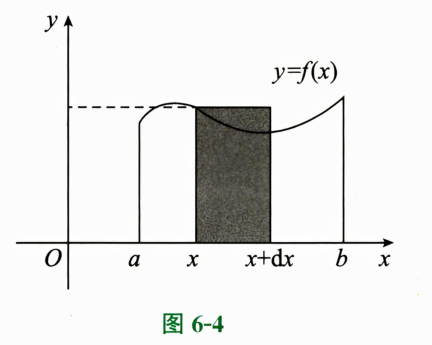
\includegraphics[width=170bp,height=135bp,keepaspectratio]{lilin-figures/第302页.png}

\vfill

\Solution

按图示取 $0\le a<b$、$f(x)\ge0$。绕 $y$ 轴旋转时，竖直小条形成薄圆柱壳。它的半径约为 $x$，圆周长为 $2\pi x$，高度为 $f(x)$，厚度为 $dx$，因此体积微元为 $dV=2\pi x f(x)\,dx$。把从 $a$ 到 $b$ 的薄壳体积累加，得到
\[
V=2\pi\int_a^b x f(x)\,dx.
\]
圆柱壳也可看作内外半径为 $x,x+dx$ 的圆环柱，其底面积 $\pi[(x+dx)^2-x^2]=2\pi x\,dx+\pi(dx)^2$，后一项在积分极限中不贡献。若曲线在横轴下方且区间仍在同一侧，壳高改取 $|f(x)|$。

\clearpage

% SOURCE line=1897 pdf_page=303 section=3.4

\Question{321}{第6章 · 例题第5组 · 例 1}

设直线 y=kx 与曲线 $y=x^{2}$ 所围图形的面积为 $S_{1}$，它们与直线 x=1 所围图形的面积为 $S_{2}$，且 k < 1.

(1) 确定 k 的值, 使得 $S_{1} + S_{2}$ 取得最小值, 并求最小值.

(2) 求该最小值所对应的图形绕 x 轴旋转一周所得旋转体的体积.

\vfill

\Solution

(1) 两曲线交于 $x=0,k$。先取 $0<k<1$，在 $[0,k]$ 直线较高，在 $[k,1]$ 抛物线较高，所以
\[
S_1+S_2=\int_0^k(kx-x^2)\,dx+\int_k^1(x^2-kx)\,dx
=\frac13-\frac k2+\frac{k^3}3.
\]
对 $k$ 求导得 $k^2-\frac12$，在 $0<k<\frac1{\sqrt2}$ 为负，在 $\frac1{\sqrt2}<k<1$ 为正，故最小点为 $k=\frac1{\sqrt2}$，最小面积 $\frac13-\frac1{3\sqrt2}$。还需检查题设允许的 $k\le0$。这时 $S_1=-\frac{k^3}6$，$S_2=\frac13-\frac k2$，总和至少为 $\frac13$，更大。

(2) 所求是两块图形的并集旋转。各处半径都是相应纵坐标，取大半径平方减小半径平方：
\[
V=\pi\int_0^k(k^2x^2-x^4)\,dx+\pi\int_k^1(x^4-k^2x^2)\,dx
=\pi\left(\frac15-\frac{k^2}3+\frac{4k^5}{15}\right).
\]
代入最小点 $k=\frac1{\sqrt2}$，得 $V=\frac{\pi(1+\sqrt2)}{30}$。

\clearpage

% SOURCE line=1905 pdf_page=304 section=3.4

\Question{322}{第6章 · 例题第5组 · 例 2}

过坐标原点作曲线 $y = \ln x$ 的切线，该切线与曲线 $y = \ln x$ 及 x 轴围成平面图形 D，如图 6-10 所示。求：

(1) D 的面积 A.

(2) D 绕直线 x = e 旋转一周所得旋转体的体积. 图6-10

\par\smallskip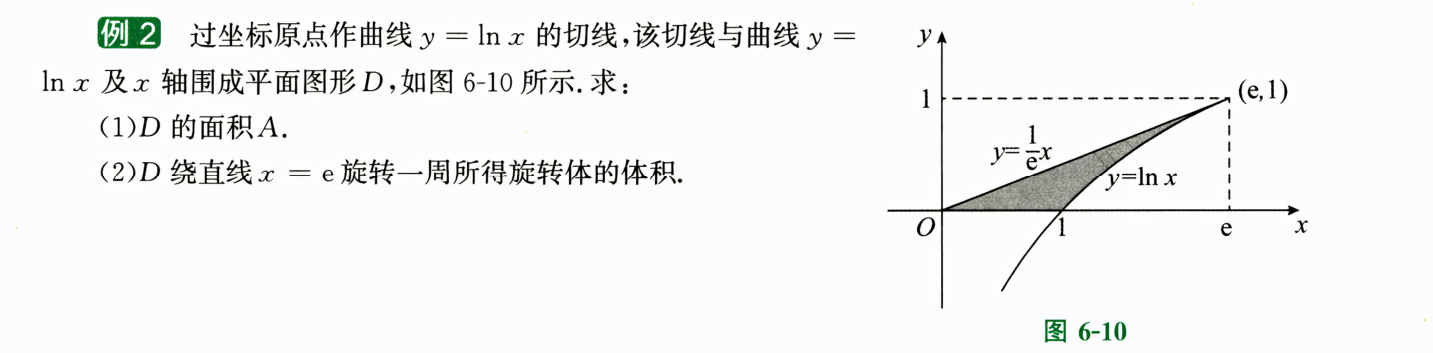
\includegraphics[width=390bp,height=135bp,keepaspectratio]{lilin-figures/第304页.png}

\vfill

\Solution

设切点横坐标为 $c$。切线为 $y=\ln c+\frac{x-c}{c}$，通过原点给出 $\ln c-1=0$，所以 $c=e$、切线为 $y=\frac xe$。

(1) $0\le x\le1$ 时图形夹在切线和横轴之间。$1\le x\le e$ 时夹在切线和对数曲线之间，因此
\[
A=\int_0^e\frac xe\,dx-\int_1^e\ln x\,dx
=\frac e2-[x\ln x-x]_1^e=\frac e2-1 .
\]
(2) 绕竖直线 $x=e$，用壳法时半径为 $e-x$。以完整切线下方的图形减去对数曲线下方的图形，得
\[
\frac{V}{2\pi}=\int_0^e(e-x)\frac xe\,dx-\int_1^e(e-x)\ln x\,dx.
\]
第一项为 $\frac{e^2}6$。第二项分别对 $\ln x$ 和 $x\ln x$ 分部，得 $-\frac{e^2}4+e-\frac14$。所以 $V=2\pi(\frac{5e^2}{12}-e+\frac14)$。

\clearpage

% SOURCE line=1924 pdf_page=307 section=3.4

\Question{323}{第6章 · 例题第5组 · 例 5}

求由摆线 $x = a(t - \sin t)$, $y = a(1 - \cos t)(a > 0)$ 的一拱 $(0 \leqslant t \leqslant 2\pi)$ 及 x 轴所围图形分别绕 x 轴，y 轴旋转一周所得旋转体的体积.

\vfill

\Solution

$x'(t)=a(1-\cos t)\ge0$，所以参数从 $0$ 走到 $2\pi$ 时不会倒行，可以直接把 $dx=a(1-\cos t)dt$ 代入体积积分。

绕 $x$ 轴用圆盘，得到 $V_x=\pi a^3\int_0^{2\pi}(1-\cos t)^3dt$。展开后，$\cos t,\cos^3t$ 在一个整周期积分为零，$\int_0^{2\pi}\cos^2t\,dt=\pi$，故 $V_x=5\pi^2a^3$。

绕 $y$ 轴用壳法，得到
\[
V_y=2\pi a^3\int_0^{2\pi}(t-\sin t)(1-\cos t)^2dt.
\]
设 $w(t)=(1-\cos t)^2$，它满足 $w(2\pi-t)=w(t)$。换元相加可得 $\int_0^{2\pi}tw(t)dt=\pi\int_0^{2\pi}w(t)dt=3\pi^2$。另有 $\int_0^{2\pi}\sin t\,w(t)dt=[\frac{(1-\cos t)^3}3]_0^{2\pi}=0$。所以 $V_y=6\pi^3a^3$。

\clearpage

% SOURCE line=1932 pdf_page=309 section=3.4

\Question{324}{第6章 · 例题第5组 · 例 7}

一个半球形容器，其半径为R。容器中盛满水，将容器中的水全部抽出容器口，至少需要做功多少？（设水的密度为$\rho=1\times10^{3}\ \frac{\mathrm{kg}}{\mathrm m^3}$，重力加速度$g=10\ \frac{\mathrm m}{\mathrm s^2}$）

\vfill

\Solution

把容器口所在水平面设为深度 $z=0$，向下为正。深度为 $z$ 的水层，到球心的竖直距离是 $z$，由球面方程得截面半径平方为 $R^2-z^2$。厚度为 $dz$ 的水层体积约为 $\pi(R^2-z^2)dz$，重力为这个体积乘 $\rho g$。

这一层水要提升 $z$，故所需功的微元是 $dW=\rho g\pi z(R^2-z^2)dz$。对全部深度累加，
\[
W=\rho g\pi\int_0^R z(R^2-z^2)\,dz
=\rho g\pi\left[\frac{R^2z^2}2-\frac{z^4}4\right]_0^R
=\frac{\rho g\pi R^4}{4}=2500\pi R^4\ \mathrm{J}.
\]
此处 $R$ 用米。每层水仅提升到容器口，给出了克服重力的最小功。

\clearpage

% SOURCE line=1936 pdf_page=310 section=3.4

\Question{325}{第6章 · 例题第5组 · 例 8}

一根长度为1的细棒位于x轴的区间[0,1]上，其线密度$\rho(x)=-x^{2}+2x+1$，求该细棒的质心坐标$\overrightarrow{x}$.

\vfill

\Solution

质心是以各小段质量为权重的平均位置。位置 $x$ 附近长度 $dx$ 的小段质量为 $dm=\rho(x)dx$，它对原点的质量矩为 $x\,dm$。所以先分别求总质量和质量矩，
\[
M=\int_0^1(-x^2+2x+1)dx=\frac53,\qquad
J=\int_0^1(-x^3+2x^2+x)dx=\frac{11}{12}.
\]
再相除，得到 $\bar x=\frac JM=\frac{11}{20}$。密度在 $[0,1]$ 上递增，右端更重，结果比均匀细棒的中点 $\frac12$ 稍靠右，且位于棒内。

\clearpage

% SOURCE line=1940 pdf_page=311 section=3.4

\Question{326}{第6章 · 例题第5组 · 例 9}

某闸门的形状与大小如图6-14所示，其中l为对称轴。闸门的上部为矩形ABCD，下部由二次抛物线与线段AB组成，当水面与闸门的上端相平时，欲使闸门矩形部分承受的水压力与闸门下部承受的水压力之比为5:4，问闸门矩形部分的高h应为多少米？

\par\smallskip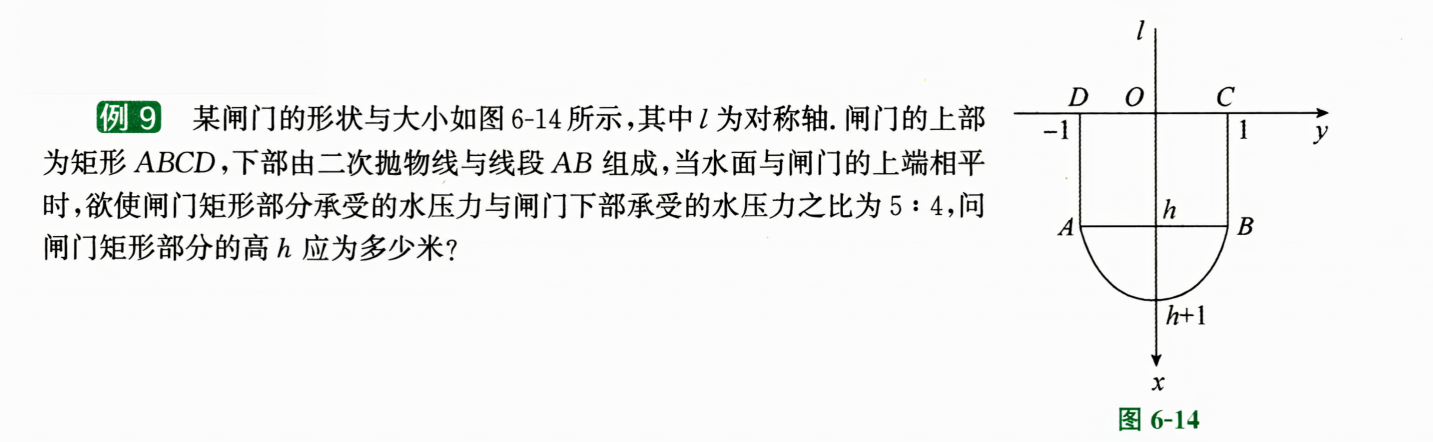
\includegraphics[width=390bp,height=135bp,keepaspectratio]{lilin-figures/第311页.png}

\vfill

\Solution

按图中标注取水平坐标 $y$，竖直向下的深度为 $z$。矩形半宽为 $1$，下方抛物线的顶点深度为 $h+1$、两端在 $(\pm1,h)$，故它的方程为 $z=h+1-y^2$。深度 $z$ 处的下部宽度是 $2\sqrt{h+1-z}$。

水压强为 $\rho gz$。水平薄条两端的深度相同，压力微元为压强乘宽度再乘 $dz$。于是
\[
F_{\text{矩}}=\rho g\int_0^h2z\,dz=\rho gh^2,\quad
F_{\text{下}}=2\rho g\int_h^{h+1}z\sqrt{h+1-z}\,dz.
\]
第二个积分令 $u=h+1-z$，得到 $F_{\text{下}}=2\rho g[\frac{2(h+1)}3-\frac25]=\rho g(\frac{4h}3+\frac8{15})$。由比值 $\frac{F_{\text{矩}}}{F_{\text{下}}}=\frac54$ 得 $3h^2-5h-2=0$，两根为 $2,-\frac13$。高度为正，故 $h=2\ \mathrm m$。

\clearpage

% SOURCE line=1946 pdf_page=312 section=3.4

\Question{327}{第6章 · 例题第5组 · 例 10}

设单位质点 P, Q 分别位于点 (0,0) 和点 (0,1) 处, P 从点 (0,0) 出发沿 x 轴正向移动, 记 G 为引力常量, 则当质点 P 移动到点 (l,0) 时, 克服质点 Q 的引力所做的功为 ( ).

\textbf{A.} $\int_{0}^{l}\frac{G}{x^{2}+1}dx$

\textbf{B.} $\int_{0}^{l}\frac{Gx}{(x^{2}+1)^{\frac{3}{2}}}dx$

\textbf{C.} $\int_{0}^{l}\frac{G}{(x^{2}+1)^{\frac{3}{2}}}dx$

\textbf{D.} $\int_{0}^{l}\frac{G(x+1)}{(x^{2}+1)^{\frac{3}{2}}}dx$

\vfill

\Solution

质点移动到 $(x,0)$ 时，与 $Q$ 的距离为 $r=\sqrt{x^2+1}$。两者都是单位质量，引力大小为 $\frac{G}{r^2}$，方向沿着从 $P$ 指向 $Q$ 的连线。

做功只计算力在移动方向上的分量。引力的水平分量朝负 $x$ 方向，其大小还要乘方向因子 $\frac{x}{r}$，所以为 $\frac{Gx}{(x^2+1)^{\frac32}}$。为克服该引力，外力沿正 $x$ 方向做功，因此
\[
W=\int_0^l\frac{Gx}{(x^2+1)^{\frac32}}\,dx
=G\left(1-\frac1{\sqrt{1+l^2}}\right).
\]
对应 \textbf{B}。因子 $\frac{x}{r}$ 来自方向投影，仅用引力大小会把竖直方向的力也计入水平功。

\clearpage

% SOURCE line=2101 pdf_page=337 section=3.4

\Question{328}{第6章 · 解答题 · 第 17 题}

设平面图形D由$x^{2}+y^{2}\leqslant2x$与$y\geqslant x$所围，求图形D绕直线x=2旋转一周所得旋转体的体积.

\vfill

\Solution

圆的方程写为 $(x-1)^2+y^2\le1$。直线与圆交于 $(0,0),(1,1)$，满足 $y\ge x$ 的部分只能位于 $0\le x\le1$，其上下边界为 $\sqrt{2x-x^2}$ 和 $x$。

绕竖直线 $x=2$，用竖条圆柱壳。半径为 $2-x$，高度为 $\sqrt{2x-x^2}-x$，所以
\[
\frac{V}{2\pi}=\int_0^1(2-x)\sqrt{2x-x^2}dx-\int_0^1(2x-x^2)dx.
\]
第二项为 $\frac23$。第一项令 $u=x-1$，得 $\int_{-1}^0(1-u)\sqrt{1-u^2}du=\frac\pi4+\frac13$，分别是单位圆四分之一面积和幂函数换元积分。相减再乘 $2\pi$，得 $V=\frac{\pi^2}2-\frac{2\pi}3$。

\clearpage

% SOURCE line=2105 pdf_page=338 section=3.4

\Question{329}{第6章 · 解答题 · 第 18 题}

求圆域 $x^{2}+(y-b)^{2} \leqslant a^{2}(b>a)$ 绕 x 轴旋转一周所得旋转体的体积.

\vfill

\Solution

按几何题中 $a$ 是正半径，$b>a$ 保证整个圆位于横轴上方。对固定 $x\in[-a,a]$，上下边界为 $y=b\pm\sqrt{a^2-x^2}$。旋转后得到圆环，其外半径为较大的纵坐标，内半径为较小的纵坐标。因此
\[
V=\pi\int_{-a}^a\big[(b+\sqrt{a^2-x^2})^2-(b-\sqrt{a^2-x^2})^2\big]dx
=4\pi b\int_{-a}^a\sqrt{a^2-x^2}dx .
\]
最后一个积分为半径 $a$ 的上半圆面积 $\frac{\pi a^2}2$，所以 $V=2\pi^2a^2b$。先作平方差能使两个根式平方与 $b^2$ 全部抵消。

\clearpage

% SOURCE line=2109 pdf_page=339 section=3.4

\Question{330}{第6章 · 解答题 · 第 19 题}

设曲线 $y = ax^{2} (a > 0, x \geqslant 0)$ 与 $y = 1 - x^{2}$ 交于点 A，过原点 O 与点 A 的直线与 $y = ax^{2}$ 围成一个平面图形，问 a 为何值时，该图形绕 x 轴旋转所得旋转体的体积最大？最大体积是多少？

\vfill

\Solution

由 $ax^2=1-x^2$，交点横坐标为 $c=\frac1{\sqrt{a+1}}$，纵坐标为 $ac^2$。过原点的直线斜率为 $ac$，所以直线方程 $y=acx$。在 $0<x<c$，直线高于 $ax^2$，旋转截面是圆环，故
\[
V(a)=\pi\int_0^c[(acx)^2-(ax^2)^2]dx
=\frac{2\pi a^2}{15(a+1)^{\frac52}}.
\]
此时 $a$ 才是待优化的变量。求导可将正因子提出，得到
\[
V'(a)=\frac{\pi a(4-a)}{15(a+1)^{\frac72}}.
\]
所以 $0<a<4$ 时递增，$a>4$ 时递减，全局最大值在 $a=4$ 取得，为 $V_{\max}=\frac{32\pi}{375\sqrt5}$。两端 $a\to0^+$、$a\to+\infty$ 的体积均趋于零。

\clearpage

% SOURCE line=2113 pdf_page=340 section=3.4

\Question{331}{第6章 · 解答题 · 第 20 题}

(仅数学一、数学二要求)设一容器的内侧是由图6-15中曲线绕y轴旋转一周而成的曲面，该曲线由$x^{2}+y^{2}=2y(y\geqslant\frac{1}{2})$与$x^{2}+y^{2}=1(y\leqslant\frac{1}{2})$连接而成.

（I）求容器的容积；

（II）若将容器内盛满的水从容器顶全部抽出，至少需要做多少功？ 图6-15

\par\smallskip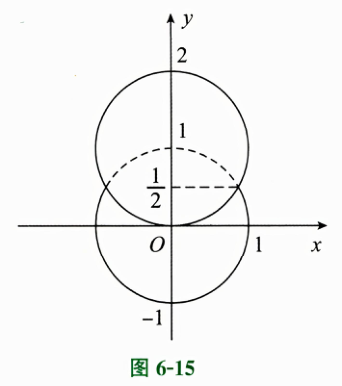
\includegraphics[width=170bp,height=135bp,keepaspectratio]{lilin-figures/第340页.png}

\vfill

\Solution

由原图，容器底部为 $y=-1$，顶部为 $y=2$。水平截面在 $y=\frac12$ 处换边界。半径平方在下部为 $1-y^2$，上部为 $2y-y^2$。

(I) 按圆盘体积累加，
\[
V=\pi\int_{-1}^{\frac12}(1-y^2)dy+
\pi\int_{\frac12}^2(2y-y^2)dy
=\pi\left(\frac98+\frac98\right)=\frac{9\pi}4.
\]
(II) 记水密度为 $\rho$、重力加速度为 $g$。高度 $y$ 处厚 $dy$ 的水层需提升 $2-y$，故功为重力乘提升高度。于是
\[
W=\rho g\pi\left[\int_{-1}^{\frac12}(2-y)(1-y^2)dy+
\int_{\frac12}^2(2-y)(2y-y^2)dy\right].
\]
两个积分分别是 $\frac{153}{64}$ 和 $\frac{63}{64}$，所以 $W=\frac{27\pi\rho g}{8}$。题干未指定 $\rho,g$ 及长度单位，保留一般式。若坐标以米计且取 $\rho=1000,g=10$，则为 $33750\pi\ \mathrm J$。

\clearpage

% SOURCE line=3129 pdf_page=530 section=3.4

\Question{332}{第10章 · 例题第2组 · 例 1}

求由抛物面 $z = 10 - 3x^{2} - 3y^{2}$ 与平面 z = 4 所围立体的体积.

\vfill

\Solution

这个立体绕 $z$ 轴对称，最方便用水平圆片计算体积。固定高度 $z$，由抛物面得 $x^2+y^2=\frac{10-z}{3}$，所以圆片半径的平方为 $\frac{10-z}{3}$，截面积为 $S(z)=\frac\pi3(10-z)$。

平面是底面 $z=4$，抛物面的最高点为 $z=10$。薄圆片的体积是截面积乘厚度，对所有高度相加得到
\[
V=\int_4^{10}S(z)\,\mathrm dz
=\frac\pi3\int_4^{10}(10-z)\,\mathrm dz
=\frac\pi3\left[10z-\frac{z^2}{2}\right]_4^{10}=6\pi.
\]
底面半径为 $\sqrt2$，截面积从 $2\pi$ 线性下降到零，高度为 $6$，平均截面积为 $\pi$，所以体积也为 $6\pi$，可作核验。

\clearpage

% SOURCE line=3275 pdf_page=554 section=3.4

\Question{333}{第10章 · 解答题 · 第 12 题}

(仅数学一要求)求两个圆柱面$x^{2}+y^{2}=R^{2}$与$x^{2}+z^{2}=R^{2}$所围立体的体积.

\vfill

\Solution

两个圆柱都限制了同一个 $x$，所以垂直于 $x$ 轴切片最直接。设 $R>0$，固定 $-R\le x\le R$，两条件分别要求 $|y|\le\sqrt{R^2-x^2}$、$|z|\le\sqrt{R^2-x^2}$。

在该平面中，$y,z$ 的限制相互独立，截面是边长 $2\sqrt{R^2-x^2}$ 的正方形，截面积 $S(x)=4(R^2-x^2)$。于是
\[
V=\int_{-R}^R4(R^2-x^2)\,\mathrm dx
=8\int_0^R(R^2-x^2)\,\mathrm dx
=\frac{16R^3}{3}.
\]
利用偶性把区间缩成一半，可减少计算。结果含 $R^3$，与体积随长度的三次方缩放一致。若将半径写作任意非零实数，应将结果的 $R$ 替换成 $|R|$。

\clearpage

% SOURCE line=4014 pdf_page=670 section=3.4

\Question{334}{第13章 · 例题第1组 · 例 6}

求由曲面 $x^{2}+y^{2}=az, z=2a-\sqrt{x^{2}+y^{2}}(a>0)$ 所围成的立体的体积.

\vfill

\Solution

两曲面都绕 $z$ 轴对称。记水平半径 $r=\sqrt{x^2+y^2}\ge0$，交线满足 $\frac{r^2}{a}=2a-r$，即 $(r-a)(r+2a)=0$。因 $r\ge0,a>0$，交圆为 $r=a,z=a$。

固定高度后，内部同时满足 $r^2\le az$ 和 $r\le2a-z$。在 $0\le z\le a$，第一条更严格，圆片面积为 $\pi az$；在 $a\le z\le2a$，第二条更严格，面积为 $\pi(2a-z)^2$。所以
\[
V=\pi\int_0^a a z\,\mathrm dz+
\pi\int_a^{2a}(2a-z)^2\,\mathrm dz
=\frac{\pi a^3}{2}+\frac{\pi a^3}{3}
=\frac{5\pi a^3}{6}.
\]
两片在 $z=a$ 都有半径 $a$，相接处的截面积连续。

\clearpage

% SOURCE line=4018 pdf_page=671 section=3.4

\Question{335}{第13章 · 例题第1组 · 例 7}

某均匀物体由上、下两部分组成，上部分是半径为a的半球体，下部分是底面半径为a、高为3的直圆锥体，且半球体的底面圆与圆锥的底面重合，问当a为何值时，此物体的重心恰好在球心位置？

\vfill

\Solution

取公共底面为 $z=0$，球心正好在原点，半球在上方、圆锥在下方。均匀密度记为 $\rho>0$。对称性保证重心在 $z$ 轴上，重心恰在球心等价于关于底面的总质量矩 $\int z\,\mathrm dm=0$。

上半球在高度 $z\in[0,a]$ 的截面积为 $\pi(a^2-z^2)$。下圆锥高度为 $3$，相似三角形给出 $-3\le z\le0$ 时截面半径 $a(1+\frac z3)$。薄片质量为 $\rho$ 乘截面积再乘厚度，所以两部分的质量矩分别为
\[
\begin{aligned}
M_+&=\rho\pi\int_0^az(a^2-z^2)\,\mathrm dz=\frac{\rho\pi a^4}{4},\\
M_-&=\rho\pi a^2\int_{-3}^0z\left(1+\frac z3\right)^2\,\mathrm dz
=-\frac{3\rho\pi a^2}{4}.
\end{aligned}
\]
令 $M_++M_-=0$，约去正因子 $\frac{\rho\pi a^2}{4}$，得到 $a^2=3$。半径为正，故 $a=\sqrt3$。下部质量矩带负号，来自下部高度 $z<0$。

\clearpage

\SectionHeading{3.5}{反常积分}

% SOURCE line=1672 pdf_page=263 section=3.5

\Question{336}{第6章 · 例题第1组 · 例 9}

设 $f(x)=\int_{1}^{x}\frac{\ln(t+1)}{t}dt$，求 $I=\int_{0}^{1}\frac{f(x)}{\sqrt{x}}dx$.

\vfill

\Solution

先处理 $0$ 处的反常性。$\frac{\ln(1+t)}t\to1$，故 $f$ 在 $0$ 附近有界，乘上 $\frac1{\sqrt x}$ 仍可积。先从 $\varepsilon>0$ 开始分部，用 $v=2\sqrt x$。当 $\varepsilon\to0^+$ 时端点积趋于零，且 $f(1)=0$，于是
\[
I=-2\int_0^1\frac{\ln(1+x)}{\sqrt x}\,dx
=-4\int_0^1\ln(1+u^2)\,du,\qquad u=\sqrt x.
\]
再分部，$\int_0^1\ln(1+u^2)\,du=\ln2-2\int_0^1(1-\frac1{1+u^2})\,du=\ln2-2+\frac\pi2$。因此 $I=8-2\pi-4\ln2$。它为负，与 $f(x)<0$ 一致。

\clearpage

% SOURCE line=1764 pdf_page=284 section=3.5

\Question{337}{第6章 · 例题第3组 · 例 4}

设 $a=\int_{0}^{\frac{\pi}{4}}\ln(\sin x)dx$, $b=\int_{0}^{\frac{\pi}{4}}\ln(\cot x)dx$, $c=\int_{0}^{\frac{\pi}{4}}\ln(\cos x)dx$, 则 a, b, c 的大小关系为().

\textbf{A.} $a < b < c$

\textbf{B.} a < c < b

\textbf{C.} b < a < c

\textbf{D.} c < b < a

\vfill

\Solution

先看收敛性。$x\to0^+$ 时，$\ln(\sin x)=\ln x+\ln(\frac{\sin x}{x})$，第二项趋于零，而 $\ln x$ 的反常积分收敛，因为 $x\ln x-x\to0$。同理 $\ln(\cot x)=\ln(\cos x)-\ln(\sin x)$ 也可积。

在 $0<x<\frac\pi4$ 上，$0<\sin x<\cos x<1$，因此 $a<c<0$。此外 $\cot x>1$，所以 $b>0$。合并得到 $a<c<b$，选 \textbf{B}。可以先在 $[\varepsilon,\frac\pi4]$ 比较，再令 $\varepsilon\to0^+$。

\clearpage

% SOURCE line=1842 pdf_page=294 section=3.5

\Question{338}{第6章 · 例题第4组 · 例 1}

设$\lim_{x\to\infty}\left(\frac{1+x}{x}\right)^{ax}=\int_{-\infty}^{a}t\mathrm{e}^{t}dt$，则a=\underline{\hspace{4em}}。

\vfill

\Solution

左边是重要极限的变形。对幂取对数得 $ax\ln(1+\frac1x)\to a$，故左边为 $e^a$。右边是无穷区间上的积分，先从有限的 $b$ 积到 $a$。对 $t e^t$ 分部，原函数为 $(t-1)e^t$。当 $b\to-\infty$，$(b-1)e^b\to0$，因此右边为 $(a-1)e^a$。

等式两边除以始终为正的 $e^a$，得 $1=a-1$，所以 $a=2$。代回，两边都等于 $e^2$。

\clearpage

% SOURCE line=1846 pdf_page=295 section=3.5

\Question{339}{第6章 · 例题第4组 · 例 2}

已知$\int_{0}^{+\infty}\frac{\sin x}{x}dx=\frac{\pi}{2}$，求$\int_{0}^{+\infty}\frac{\sin^{2}x}{x^{2}}dx$。

\vfill

\Solution

已知的是分母一次幂的积分，所求分母二次幂。分部积分时让 $\frac1{x^2}$ 积成 $-\frac1x$，就能降低分母次数。先在 $[\varepsilon,R]$ 上计算，
\[
\int_\varepsilon^R\frac{\sin^2 x}{x^2}\,dx
=\left[-\frac{\sin^2x}{x}\right]_\varepsilon^R
+\int_\varepsilon^R\frac{\sin 2x}{x}\,dx .
\]
$R\to+\infty$ 时分子有界，边界项趋于零。$\varepsilon\to0^+$ 时 $\sin^2\varepsilon$ 约为 $\varepsilon^2$，边界项也趋于零。最后令 $u=2x$，$\frac{dx}{x}=\frac{du}{u}$，所求正好等于给出的 $\frac\pi2$。

\clearpage

% SOURCE line=1850 pdf_page=296 section=3.5

\Question{340}{第6章 · 例题第4组 · 例 3}

判别下列反常积分的敛散性：

(1)$\int_{1}^{+\infty}\frac{\mathrm{d}x}{x^{2}\sqrt{1+x}}$; (2)$\int_{0}^{1}\frac{\mathrm{d}x}{\ln(1+x)}$.

\vfill

\Solution

(1) 上限为无穷大。对 $x\ge1$，$0<\frac1{x^2\sqrt{1+x}}\le\frac1{x^{\frac52}}$。右边的幂积分收敛，因为指数 $\frac52>1$。用比较准则得原积分收敛。

(2) 这里的问题在 $x=0$。对 $x>0$，$\ln(1+x)\le x$，这可由 $x-\ln(1+x)$ 在 $0$ 处为零且导数非负看出。所以 $\frac1{\ln(1+x)}\ge\frac1x$。而 $\int_\varepsilon^1\frac{dx}{x}=-\ln\varepsilon\to+\infty$，比较得原积分发散至 $+\infty$。

\clearpage

% SOURCE line=1856 pdf_page=297 section=3.5

\Question{341}{第6章 · 例题第4组 · 例 4}

下列反常积分收敛的是( ).

\textbf{A.} $\int_{-\infty}^{+\infty}\frac{x}{1+x^{2}}\mathrm{d}x$

\textbf{B.} $\int_{2}^{+\infty}\frac{\ln x}{x}\mathrm{d}x$

\textbf{C.} $\int_{2}^{+\infty}\frac{\mathrm{d}x}{x\ln x}$

\textbf{D.} $\int_{2}^{+\infty}\frac{x}{\mathrm{e}^{x}}\mathrm{d}x$

\vfill

\Solution

逐项在有限区间求原函数，再检查无穷端。

A 的原函数为 $\frac12\ln(1+x^2)$。$[0,+\infty)$ 上已发散，整轴积分也发散。奇函数两边对称抵消只会得到主值。

B 的原函数为 $\frac12(\ln x)^2$，趋于无穷。C 的原函数为 $\ln\ln x$，同样趋于无穷。

D 的原函数为 $-(x+1)e^{-x}$，在 $+\infty$ 趋于 $0$。因此积分等于 $3e^{-2}$，为有限值，选 \textbf{D}。

\clearpage

% SOURCE line=1868 pdf_page=298 section=3.5

\Question{342}{第6章 · 例题第4组 · 例 5}

计算下列积分：

(1) $I=\int_{\frac{1}{2}}^{\frac{3}{2}} \frac{\mathrm{d}x}{\sqrt{|x-x^2|}};$ (2) $I=\int_{1}^{+\infty} \frac{\mathrm{d}x}{x \sqrt{x-1}}.$

\vfill

\Solution

\TextCorrection{对照原页，第一问的根号写成 $\sqrt{|x-x^2|}$，删除 OCR 多出的 $1$。}
(1) 先在唯一的奇点 $1$ 处分开。左边 $|x-x^2|=x(1-x)$，令 $x=\sin^2 t$ 后被积式为 $2dt$，$t$ 从 $\frac\pi4$ 到 $\frac\pi2$，得到 $\frac\pi2$。右边 $|x-x^2|=x(x-1)$，令 $u=\sqrt{x-1}$ 后化成 $\int_0^{\frac1{\sqrt2}}\frac{2}{\sqrt{1+u^2}}du$，得 $2\ln(\frac{1+\sqrt3}{\sqrt2})=\ln(2+\sqrt3)$。两段都收敛，总值 $\frac\pi2+\ln(2+\sqrt3)$。

(2) 同样令 $u=\sqrt{x-1}$，上下限变为 $0,+\infty$，积分化为 $\int_0^{+\infty}\frac{2}{1+u^2}du=2(\frac\pi2-0)=\pi$。这个换元同时化解了下端点的根号奇性。

\clearpage

% SOURCE line=1874 pdf_page=299 section=3.5

\Question{343}{第6章 · 例题第4组 · 例 6}

设$\int_{0}^{+\infty}f(x)dx$收敛，且$f(x)=\frac{1}{1+x^{2}}-\frac{e^{-x}}{1+e^{x}}\int_{0}^{+\infty}f(x)dx$，求$\int_{0}^{+\infty}f(x)dx$。

\vfill

\Solution

将未知的积分记作 $I$。右边是关于这个常数的线性式，因此把等式两边都对 $x$ 积分，就能解出 $I$。第一项的积分为 $\frac\pi2$。第二项令 $u=e^{-x}$，得
\[
\int_0^{+\infty}\frac{e^{-x}}{1+e^x}dx
=\int_0^1\frac{u}{1+u}du=1-\ln2 .
\]
两项均收敛，可以分别积分。于是 $I=\frac\pi2-I(1-\ln2)$，整理得 $I=\frac{\pi}{2(2-\ln2)}$。$2-\ln2>0$，方程有唯一解。

\clearpage

% SOURCE line=1878 pdf_page=300 section=3.5

\Question{344}{第6章 · 例题第4组 · 例 7}

已知$\int_{1}^{+\infty}\left(\frac{2x^{2}+ax+b}{2x^{2}+bx}-1\right)dx=1(b>0)$，求a，b的值.

\vfill

\Solution

先合并被积式为 $\frac{(a-b)x+b}{x(2x+b)}$。若 $a\ne b$，用它乘 $x$ 后极限是非零的 $\frac{a-b}{2}$，所以尾部与常数倍的 $\frac1x$ 同号且同阶，积分发散。题目给出有限值，必须 $a=b$。

此时被积式拆为 $\frac1x-\frac2{2x+b}$，先积到 $R$ 再令 $R\to+\infty$，得到
\[
\lim_{R\to+\infty}[\ln x-\ln(2x+b)]_1^R=\ln(1+\frac b2).
\]
令它等于 $1$，得到 $a=b=2(e-1)$，满足 $b>0$，且在积分区间分母不为零。

\clearpage

% SOURCE line=1882 pdf_page=301 section=3.5

\Question{345}{第6章 · 例题第4组 · 例 8}

设$\int_{1}^{+\infty}\frac{a}{x(2x+a)}\mathrm{d}x=\ln2$，则a=\underline{\hspace{4em}}。

\vfill

\Solution

先检查分母。若 $a\le-2$，则 $2x+a$ 在区间内或端点为零，且 $a\ne0$，出现一阶极点，积分发散。故只考虑 $a>-2$。把分式拆开，正好得到两个对数导数：
\[
\frac{a}{x(2x+a)}=\frac1x-\frac2{2x+a}.
\]
积分到 $R$，合并成 $\ln\frac{x}{2x+a}$ 再代入端点。$R\to+\infty$ 时 $\frac{R}{2R+a}\to\frac12$，所以积分为 $\ln(1+\frac a2)$。由 $\ln(1+\frac a2)=\ln2$，得到 $a=2$。

\clearpage

% SOURCE line=1916 pdf_page=305 section=3.5

\Question{346}{第6章 · 例题第5组 · 例 3}

求曲线 $y = e^{-x} \sqrt{\sin x}$ ($x \geqslant 0$) 绕 x 轴旋转一周所得旋转体的体积 V.

\vfill

\Solution

平方根要求 $\sin x\ge0$，因此实数曲线只存在于各段 $[2k\pi,(2k+1)\pi]$，$k=0,1,\ldots$。每一段与横轴之间的图形绕横轴形成旋转体，截面面积为 $\pi y^2=\pi e^{-2x}\sin x$。

第一段体积除以 $\pi$ 为
\[
J=\int_0^\pi e^{-2x}\sin x\,dx
=\left[-\frac{e^{-2x}(2\sin x+\cos x)}5\right]_0^\pi
=\frac{1+e^{-2\pi}}5.
\]
第 $k$ 段通过平移 $x=2k\pi+u$，其体积等于 $\pi J e^{-4k\pi}$。前 $N$ 段的体积用有限等比数列公式相加，令 $N\to+\infty$，得到 $V=\frac{\pi J}{1-e^{-4\pi}}=\frac{\pi}{5(1-e^{-2\pi})}$。

\clearpage

% SOURCE line=1998 pdf_page=316 section=3.5

\Question{347}{第6章 · 选择题 · 第 4 题}

下列反常积分发散的是( ).

\textbf{A.} $\int_{0}^{+\infty}x\mathrm{e}^{-x}\mathrm{d}x$

\textbf{B.} $\int_{0}^{+\infty}x\mathrm{e}^{-x^{2}}\mathrm{d}x$

\textbf{C.} $\int_{0}^{+\infty}\frac{\arctan x}{1+x^{2}}\mathrm{d}x$

\textbf{D.} $\int_{0}^{+\infty}\frac{x}{1+x^{2}}\mathrm{d}x$

\vfill

\Solution

先对各项积到有限的上限 $R$，然后令 $R\to+\infty$。

A 对 $x e^{-x}$ 分部，得到 $[-(x+1)e^{-x}]_0^R\to1$，收敛。

B 用 $u=x^2$，得到 $\frac12\int_0^{R^2}e^{-u}du\to\frac12$，收敛。

C 用 $u=\arctan x$，得到 $\frac12(\arctan R)^2\to\frac{\pi^2}{8}$，收敛。

D 的原函数为 $\frac12\ln(1+x^2)$，在 $R\to+\infty$ 时趋于 $+\infty$，所以发散，选 \textbf{D}。前三项不仅有有限极限，还给出了各自的积分值。

\clearpage

% SOURCE line=2042 pdf_page=324 section=3.5

\Question{348}{第6章 · 解答题 · 第 4 题}

求下列积分: (I) $\int_{-1}^{1}\frac{2x^{2}+\sin x}{1+\sqrt{1-x^{2}}}\mathrm{d}x;$ (II) $\int_{0}^{n\pi}\sqrt{1-\sin2x}\mathrm{d}x;$ (III) $\int_{0}^{1}\frac{x\mathrm{d}x}{(2-x^{2})\sqrt{1-x^{2}}};$

(IV) $\int_{0}^{\frac{\pi}{2}}\ln(\sin x)\mathrm{d}x;$ (V) $\int_{0}^{\frac{\pi}{4}}\frac{x}{1+\cos2x}\mathrm{d}x;$ (VI) $\int_{\frac{1}{2}}^{2}\left(1+x-\frac{1}{x}\right)\mathrm{e}^{x+\frac{1}{x}}\mathrm{d}x;$

(VII) $\int_{-\mathrm{e}}^{-\sqrt{\mathrm{e}}}\frac{\ln\ln|x|}{x\ln|x|}\mathrm{d}x;$ (VIII) $\int_{-1}^{1}(x^{2})^{\frac{3}{2}}\mathrm{d}x.$

\vfill

\Solution

(I) 积分区间 $[-1,1]$ 关于 $0$ 对称，先检查各项的奇偶性。分母只含 $x^2$，换成 $-x$ 后不变，而 $\sin(-x)=-\sin x$，所以
\[
\int_{-1}^1\frac{\sin x}{1+\sqrt{1-x^2}}\,dx=0.
\]
这可以通过负半段令 $x=-t$ 来核对，负半段恰好是正半段的相反数。余下的分子是 $2x^2$，想到用平方差 $1-(\sqrt{1-x^2})^2=x^2$ 消去分母的根号。于是
\[
\frac{2x^2}{1+\sqrt{1-x^2}}=2(1-\sqrt{1-x^2}),\qquad
I_1=2\int_{-1}^1 1\,dx-2\int_{-1}^1\sqrt{1-x^2}\,dx.
\]
第一个积分等于区间长度 $2$。第二个积分的曲线满足 $x^2+y^2=1$、$y\ge0$，所围面积是半径 $1$ 的上半圆面积 $\frac\pi2$。所以 $I_1=2\cdot2-2\cdot\frac\pi2=4-\pi$。

(II) 根号下的 $1-\sin2x$ 可以配成一个完全平方，因为
\[
(\sin x-\cos x)^2=\sin^2x+\cos^2x-2\sin x\cos x=1-\sin2x.
\]
因此被积函数是 $|\sin x-\cos x|$。平方根取非负值，所以必须保留绝对值。这个函数的周期是 $\pi$，因为 $x$ 增加 $\pi$ 后括号内整体变号，绝对值不变。当 $n$ 为正整数时，$[0,n\pi]$ 包含 $n$ 个完整周期，每一段的积分相同。

先计算 $[0,\pi]$。其中 $\sin x-\cos x$ 在 $\frac\pi4$ 处为零，在左段为负、右段为正，所以
\[
\begin{aligned}
J&=\int_0^{\frac\pi4}(\cos x-\sin x)\,dx+
\int_{\frac\pi4}^{\pi}(\sin x-\cos x)\,dx\\
&=[\sin x+\cos x]_0^{\frac\pi4}
+[-\cos x-\sin x]_{\frac\pi4}^{\pi}\\
&=(\sqrt2-1)+(1+\sqrt2)=2\sqrt2.
\end{aligned}
\]
累加 $n$ 段，得到 $I_2=nJ=2\sqrt2\,n$。

(III) 根号内是 $1-x^2$，其导数含 $x$，恰好与分子的 $x\,dx$ 配合，故令 $u=\sqrt{1-x^2}$。平方后有 $u^2=1-x^2$，微分得 $2u\,du=-2x\,dx$，即 $x\,dx=-u\,du$。另外，$2-x^2=1+u^2$。代入后，分子中的 $u$ 与分母的根号 $u$ 相消，只剩下
\[
\frac{x\,dx}{(2-x^2)\sqrt{1-x^2}}=-\frac{du}{1+u^2}.
\]
原积分在 $x=1$ 处有奇性，先把上限取为 $b<1$。$x=0$ 时 $u=1$，$x=b$ 时 $u=\sqrt{1-b^2}$，因此
\[
\int_0^b\frac{x\,dx}{(2-x^2)\sqrt{1-x^2}}
=-\int_1^{\sqrt{1-b^2}}\frac{du}{1+u^2}
=\arctan1-\arctan\sqrt{1-b^2}.
\]
令 $b\to1^-$，第二项趋于 $0$，得到 $I_3=\frac\pi4$。这个有限极限也证明反常积分收敛。

(IV) 记 $J=\int_0^{\frac\pi2}\ln(\sin x)\,dx$。先检查反常端点 $0$。由 $\frac{\sin x}{x}\to1$，有
\[
\ln(\sin x)=\ln x+\ln\frac{\sin x}{x},\qquad
\ln\frac{\sin x}{x}\longrightarrow0.
\]
后面的修正项在 $0$ 附近有界，而 $\int_\varepsilon^\delta\ln x\,dx=[x\ln x-x]_\varepsilon^\delta$ 在 $\varepsilon\to0^+$ 时有有限极限，因为 $\varepsilon\ln\varepsilon\to0$。所以 $J$ 收敛，以下的拆分、换元和相加都有依据。

直接求 $\ln\sin x$ 的原函数困难，看到区间端点为 $0,\frac\pi2$，可想到用 $x=\frac\pi2-t$ 将正弦换成余弦。此时 $dx=-dt$，上下限依次为 $\frac\pi2,0$，翻转上下限后得到
\[
J=\int_0^{\frac\pi2}\ln(\cos t)\,dt.
\]
将两份相等的积分相加。区间内部正弦、余弦都为正，故对数可以合并，再用 $\sin x\cos x=\frac12\sin2x$：
\[
2J=\int_0^{\frac\pi2}\ln(\sin x\cos x)\,dx
=\int_0^{\frac\pi2}\ln(\sin2x)\,dx-\frac\pi2\ln2.
\]
设这里的新积分为 $K$。令 $u=2x$，则 $dx=\frac12du$，上下限变为 $0,\pi$，所以
\[
K=\frac12\left[\int_0^{\frac\pi2}\ln(\sin u)\,du+
\int_{\frac\pi2}^{\pi}\ln(\sin u)\,du\right].
\]
前一项就是 $J$。后一项令 $v=\pi-u$，利用 $\sin(\pi-v)=\sin v$，也得到 $J$。因此 $K=\frac12(J+J)=J$。代回得到 $2J=J-\frac\pi2\ln2$，移项即得 $I_4=J=-\frac\pi2\ln2$。

(V) 分母含 $1+\cos2x$，先用二倍角公式 $1+\cos2x=2\cos^2x$，得到
\[
I_5=\frac12\int_0^{\frac\pi4}x\sec^2x\,dx.
\]
这里 $x$ 求导后会变成 $1$，而 $\sec^2x$ 容易积分为 $\tan x$，适合分部积分。取 $U=x$、$dV=\sec^2x\,dx$，则 $dU=dx$、$V=\tan x$，从而
\[
I_5=\frac12[x\tan x]_0^{\frac\pi4}
-\frac12\int_0^{\frac\pi4}\tan x\,dx.
\]
因 $\frac{d}{dx}\ln(\cos x)=-\tan x$，余下积分为 $[-\ln(\cos x)]_0^{\frac\pi4}=\frac12\ln2$。端点项为 $\frac\pi4\cdot1-0=\frac\pi4$，故 $I_5=\frac\pi8-\frac{\ln2}{4}$。

(VI) 指数为 $h(x)=x+\frac1x$，求导得到 $h'(x)=1-\frac1{x^2}$。指数函数求导时会出现这个因子，但题目中的因子为 $1+x-\frac1x$。其中 $x-\frac1x=xh'(x)$，余下的 $1$ 提示再乘一个 $x$，利用乘积法则产生它：
\[
\frac{d}{dx}\bigl(xe^{h(x)}\bigr)
=e^{h(x)}+xe^{h(x)}h'(x)
=\left(1+x-\frac1x\right)e^{x+\frac1x}.
\]
所以原函数为 $xe^{x+\frac1x}$。积分区间内 $x>0$，该原函数处处可导。两个端点的指数相同，$2+\frac12=\frac12+2=\frac52$，因此
\[
I_6=\left[xe^{x+\frac1x}\right]_{\frac12}^2
=2e^{\frac52}-\frac12e^{\frac52}
=\frac32e^{\frac52}.
\]

(VII) 被积式有两层对数，先从内层 $\ln|x|$ 入手，因为分母中恰好有它的导数 $\frac1x$。令 $u=\ln|x|$，则 $du=\frac{dx}{x}$。原区间中 $x<0$，$|x|$ 从 $e$ 变到 $\sqrt e$，所以 $u$ 从 $1$ 变到 $\frac12$。这时 $u>0$，外层的 $\ln u$ 也有定义。代换后
\[
I_7=\int_1^{\frac12}\frac{\ln u}{u}\,du.
\]
再令 $v=\ln u$，则 $dv=\frac{du}{u}$，上下限从 $1,\frac12$ 变成 $0,-\ln2$，所以
\[
I_7=\int_0^{-\ln2}v\,dv
=\left[\frac{v^2}{2}\right]_0^{-\ln2}
=\frac12(\ln2)^2.
\]
两次换元都已经保留相应的积分方向，无需另加负号。原区间上分子、分母都为负，被积函数为正，与结果一致。

(VIII) 分数指数 $\frac32$ 表示先开平方再取三次幂。对负 $x$，$\sqrt{x^2}$ 也取非负值，因此
\[
(x^2)^{\frac32}=(\sqrt{x^2})^3=|x|^3.
\]
$|x|^3$ 是偶函数，在 $[-1,0]$ 与 $[0,1]$ 上的积分相同。只算正半段再乘 $2$：
\[
I_8=2\int_0^1x^3\,dx
=2\left[\frac{x^4}{4}\right]_0^1
=2\left(\frac14-0\right)=\frac12.
\]

\clearpage

% SOURCE line=2087 pdf_page=334 section=3.5

\Question{349}{第6章 · 解答题 · 第 14 题}

计算反常积分：

(I)$\int_{2}^{+\infty}\frac{\mathrm{d}x}{(x-1)^4\sqrt{x^2-2x}}$; (II)$\int_{1}^{3}\frac{dx}{\sqrt{(x-1)(3-x)}}$.

\vfill

\Solution

(I) 将根号配成 $\sqrt{(x-1)^2-1}$。倒数代换 $u=\frac1{x-1}$ 同时降低分母幂并把无穷上限化为有限端点。$dx=-\frac{du}{u^2}$，原积分变为
\[
\int_0^1\frac{u^3}{\sqrt{1-u^2}}du.
\]
再令 $v=1-u^2$，变为 $\frac12\int_0^1(1-v)v^{-\frac12}dv=\frac12(2-\frac23)=\frac23$。$v^{-\frac12}$ 在 $0$ 可积，说明反常端点收敛。

(II) 根号内 $(x-1)(3-x)=1-(x-2)^2$。先把端点截去，再用反正弦原函数 $\arcsin(x-2)$，最后两端分别趋于 $\pm1$，得到 $\frac\pi2-(-\frac\pi2)=\pi$。两端的单侧积分均收敛，才能相加。

\clearpage

% SOURCE line=2097 pdf_page=336 section=3.5

\Question{350}{第6章 · 解答题 · 第 16 题}

求曲线 $y = e^{-x} \sin x \, (x \geqslant 0)$ 与 x 轴所围图形的面积.

\vfill

\Solution

面积要累加每段的正面积，故为 $A=\int_0^{+\infty}e^{-x}|\sin x|dx$。若直接积 $e^{-x}\sin x$，横轴下方的面积会被扣除。

在第 $k$ 段 $[k\pi,(k+1)\pi]$ 令 $x=k\pi+u$，则 $|\sin x|=\sin u$、$0\le u\le\pi$，所以这段面积为 $e^{-k\pi}J$，其中
\[
J=\int_0^\pi e^{-u}\sin u\,du
=\left[-\frac{e^{-u}(\sin u+\cos u)}2\right]_0^\pi
=\frac{1+e^{-\pi}}2.
\]
先累加前 $N$ 段，用有限等比和得到 $J\frac{1-e^{-N\pi}}{1-e^{-\pi}}$，令 $N\to+\infty$，得到 $A=\frac{e^\pi+1}{2(e^\pi-1)}$。

\clearpage

\clearpage\pdfbookmark[0]{第4章 常微分方程}{c4}

\SectionHeading{4.1}{几类简单的微分方程}

% SOURCE line=2159 pdf_page=346 section=4.1

\Question{351}{第7章 · 例题第1组 · 例 3}

设某商品的最大需求量为1200件，该商品的需求函数$Q=Q(P)$，需求弹性$\eta=\frac{P}{120-P}(\eta>0)$，P为单价（万元）.

(1) 求需求函数的表达式;

(2) 求 P = 100 万元时的边际收益，并说明其经济意义.

\vfill

\Solution

需求弹性的定义是 $\eta=-\frac{P}{Q}Q'$。代入后得 $\frac{Q'}Q=-\frac1{120-P}$。分离变量并积分，得到 $\ln Q=\ln(120-P)+C$，即 $Q=A(120-P)$，其中 $0<P<120$。最大需求量在价格降至零时取得，因此 $120A=1200$，$A=10$，故 $Q=1200-10P$。

“边际收益”指多卖一件时收入大约增加多少，计算的是 $\frac{\mathrm dR}{\mathrm dQ}$。把单价写成销量的函数，$P=120-\frac Q{10}$，收入为 $R=PQ=120Q-\frac{Q^2}{10}$，故边际收益为 $120-\frac Q5$。

价格为 $100$ 万元时，销量 $Q=200$，边际收益是 $80$ 万元每件，即在该销量附近每多售一件，收入约增加 $80$ 万元。

\clearpage

% SOURCE line=2193 pdf_page=352 section=4.1

\Question{352}{第7章 · 解答题 · 第 2 题}

设某种商品的社会需求量 Q = Q(P)(P 表示价格)，其弹性 $E_{d} = \frac{2P^{2}}{256 - P^{2}}(E_{d} > 0)$，当 P = 10 时，Q = 156，一个工厂生产这种商品，其日总成本函数 $C(Q) = 4Q + 2000$，求该厂日产量 Q 为多少时，总利润最大.

\vfill

\Solution

先用弹性恢复需求函数。$E_d=-\frac{P}{Q}Q'$ 给出 $\frac{Q'}Q=-\frac{2P}{256-P^2}$。积分得 $Q=A(256-P^2)$，代入 $P=10,Q=156$ 得 $A=1$，所以 $Q=256-P^2$，有效价格区间为 $0<P<16$。

利润是销售收入减成本。以 $P$ 为自变量，$\Pi(P)=(P-4)(256-P^2)-2000$。求导得 $\Pi'=256+8P-3P^2=-3(P-\frac{32}{3})(P+8)$。因此在有效区间内，利润先增后减，唯一最大值点为 $P=\frac{32}{3}$。

对应日产量为 $Q=256-(\frac{32}{3})^2=\frac{1280}{9}$ 件，约 $142.22$ 件。这是连续模型的最优值。若实际日产量限整数，比较邻近的 $142$ 与 $143$ 件，$142$ 件的利润较高，取 $142$ 件。

\clearpage

% SOURCE line=2201 pdf_page=354 section=4.1

\Question{353}{第7章 · 解答题 · 第 4 题}

设某商品的需求量 Q 对价格 P 的弹性为 $P \ln 3$，若商品的市场最大需求量为 1500 件，求需求函数。

\vfill

\Solution

把需求弹性写成定义，$-\frac{P}{Q}\frac{\mathrm dQ}{\mathrm dP}=P\ln3$。在正价格处约去 $P$，得 $\frac{Q'}Q=-\ln3$。这是可以分离变量的一阶微分方程。

两边积分，得到 $\ln Q=-P\ln3+C$，所以 $Q=A\mathrm e^{-P\ln3}=A\cdot3^{-P}$。价格越低，需求越大，最大需求量是价格趋于零时的 $A$。题给最大需求为 $1500$，所以 $Q(P)=1500\cdot3^{-P}$，$P\geq0$。

检查 $Q'=-Q\ln3$，代回弹性定义得 $P\ln3$，与已知一致。

\clearpage

% SOURCE line=2602 pdf_page=429 section=4.1

\Question{354}{第9章 · 示例 · 示例}

求微分方程 $xydx + (x^{2} + 1)dy = 0$ 的通解.

\vfill

\Solution

先把含 $\mathrm dy$ 的项留在一边。由于 $1+x^2$ 从不为零，原式可写成 $y'=-\frac{x}{1+x^2}y$。变量已经分开，或直接把它看作一阶线性齐次方程。

$\frac{x}{1+x^2}$ 的积分容易算，因为分母的导数是 $2x$。因此取积分因子 $\sqrt{1+x^2}$，由乘积求导有
\[
\frac{\mathrm d}{\mathrm dx}\bigl(\sqrt{1+x^2}\,y\bigr)
=\sqrt{1+x^2}\left(y'+\frac{x}{1+x^2}y\right)=0.
\]
括号中的整个乘积为常数，所以 $y=\frac{C}{\sqrt{1+x^2}}$，其中 $C$ 为任意实数。这里从头到尾没有除以 $y$，所以 $C=0$ 给出的零解也在内。

\clearpage

% SOURCE line=2606 pdf_page=430 section=4.1

\Question{355}{第9章 · 示例 · 示例}

求微分方程 $x \frac{\mathrm{d}y}{\mathrm{d}x} - y = 2 \sqrt{xy} \quad (x > 0)$ 的通解.

\vfill

\Solution

左边 $xy'-y$ 正好出现在 $\frac{y}{x}$ 的求导公式中，令 $z=\frac yx$。因 $x>0$，根号要求 $z\ge0$。代入 $y=xz$ 得 $xz'=2\sqrt z$。

在 $z>0$ 的区间令 $u=\sqrt z$，有 $xu'=1$，故 $u=\ln x+C$。写成 $u=\ln\frac xa$ 后，$a=\mathrm e^{-C}>0$，正值支是 $y=x(\ln\frac xa)^2$，适用 $x>a$。不能把它直接用到 $x<a$，因为此时 $\ln\frac xa<0$，与 $u=\sqrt z$ 冲突。

零解也是解。由于 $z'\ge0$，它可以先一直为零，在某个 $a>0$ 开始增长。因此整个 $(0,+\infty)$ 上的解是零解或 $y=x\bigl(\max\{0,\ln\frac xa\}\bigr)^2$。在拼接点 $a$ 两侧导数都为零，代回原式成立。局部解是这些解在相应区间的限制。

\clearpage

% SOURCE line=2610 pdf_page=431 section=4.1

\Question{356}{第9章 · 示例 · 示例}

求微分方程 $y'+\frac{1}{x}y=\frac{1}{x^{2}}\cdot y^{2}$ 满足 $y(1)=1$ 的特解.

\vfill

\Solution

题中 $y^2$ 使原方程不是线性的，但把各项除以 $y^2$ 后会出现 $\frac{y'}{y^2}$，这正是倒数求导差一个负号。初值 $y(1)=1$ 保证 $1$ 附近可设 $u=\frac1y$，得到 $u'-\frac ux=-\frac1{x^2}$。

在 $x>0$ 上乘积分因子 $\frac1x$，左边就是 $\bigl(\frac ux\bigr)'$，故 $\frac ux=\frac1{2x^2}+C$。用 $u(1)=1$ 得 $C=\frac12$，所以
\[
y=\frac{1}{\frac1{2x}+\frac x2}=\frac{2x}{1+x^2},\qquad x>0.
\]
分母始终为正，所得 $y$ 在所求区间不为零，倒数代换有效。代回 $x=1$ 恰得 $1$。

\clearpage

% SOURCE line=2614 pdf_page=432 section=4.1

\Question{357}{第9章 · 示例 · 示例}

求微分方程$(y - x^2)dx + (x - 1)dy = 0$ 的通解.

\vfill

\Solution

观察 $(x-1)y'+y$，两项恰好等于 $\bigl[(x-1)y\bigr]'$。利用这个乘积结构可以跳过寻找积分因子，直接得 $\bigl[(x-1)y\bigr]'=x^2$。

积分得到 $(x-1)y=\frac{x^3}{3}+C$，故在不含 $1$ 的区间，通解是 $y=\frac{x^3+3C}{3(x-1)}$。

如果还要求解穿过 $x=1$ 并保持有限，那么分子也须在 $1$ 处消失，即 $C=-\frac13$。约去 $x-1$ 后为 $y=\frac{x^2+x+1}{3}$，它在 $x=1$ 的值为 $1$，也符合原方程在该点给出的条件。

\clearpage

% SOURCE line=2620 pdf_page=433 section=4.1

\Question{358}{第9章 · 例题第1组 · 例 1}

已知下列各曲线族$(C,C_{1},C_{2}$ 为任意常数)，求出它们对应的微分方程：

(1)$(x-C)^{2}+y^{2}=1;$ (2)$xy=C_{1}e^{x}+C_{2}e^{-x}$

\vfill

\Solution

思路是把含任意常数的曲线关系求导，再用方程消去常数。常数在求导时视为固定。

（1）对 $(x-C)^2+y^2=1$ 求导，得 $x-C=-yy'$。把它代回原式得 $y^2(1+y'^2)=1$。这个方程不含 $C$，每一段可写成可导函数的原曲线都满足它。

（2）先把 $xy$ 看成一个整体 $u$。因为 $\mathrm e^x$ 与 $\mathrm e^{-x}$ 各求两次导数都会回到自己，所以 $u''=u$，两个常数同时消去。展开 $(xy)''=xy''+2y'$，得到 $xy''+2y'-xy=0$。

\clearpage

% SOURCE line=2626 pdf_page=434 section=4.1

\Question{359}{第9章 · 例题第1组 · 例 2}

设 $y_{1}, y_{2}$ 是一阶非齐次线性微分方程 $y' + P(x)y = Q(x)$ 的两个解，若常数 $\lambda, \mu$ ，使得 $\lambda y_{1} + \mu y_{2}$ 是该微分方程的解，$\lambda y_{1} - \mu y_{2}$ 是对应齐次微分方程的解，求 $\lambda$ 和 $\mu$ 的值.

\vfill

\Solution

记 $L[y]=y'+Py$。关键是导数和乘以 $P$ 都可以逐项分配，所以 $L[\lambda y_1\pm\mu y_2]=(\lambda\pm\mu)Q$。一条组合要保持右边为 $Q$，另一条组合要使右边为零。

当 $Q$ 不恒为零时，取一个 $Q(x)\ne0$ 的点约掉 $Q(x)$，得到 $\lambda+\mu=1$、$\lambda-\mu=0$。两式相加和相减，得 $\lambda=\mu=\frac12$。

检查：两个解取平均，右边仍为 $Q$；取半差，右边恰好抵消。若允许 $Q\equiv0$，两条条件对任意 $\lambda,\mu$ 都成立，因此这时不能确定它们；题中的“非齐次”正排除了这种退化情况。

\clearpage

% SOURCE line=2630 pdf_page=435 section=4.1

\Question{360}{第9章 · 例题第1组 · 例 3}

求微分方程 $xy' + 2y = x \ln x$ 满足 $y(1) = -\frac{1}{9}$ 的特解.

\vfill

\Solution

初值位于 $x=1$，且 $\ln x$ 要求 $x>0$。先除以 $x$ 得 $y'+\frac{2}{x}y=\ln x$。找一个因子使左边变成乘积导数。$x^2$ 的导数是 $2x$，所以乘 $x^2$ 后得到 $(x^2y)'=x^2\ln x$。

分部积分时让 $\ln x$ 求导、$x^2$ 积分，因为这样会消去对数：
\[
x^2y=\frac{x^3}{3}\ln x-\frac{x^3}{9}+C.
\]
令 $x=1$，有 $-\frac19=-\frac19+C$，所以 $C=0$。特解为 $y=\frac{x}{3}\ln x-\frac{x}{9}$。求导代回，左边 $xy'+2y=x\ln x$，正好恢复右边。

\clearpage

% SOURCE line=2634 pdf_page=436 section=4.1

\Question{361}{第9章 · 例题第1组 · 例 4}

求微分方程 $y\mathrm{d}x + (x - 3y^2)\mathrm{d}y = 0$ 满足 $y(1) = 1$ 的特解.

\vfill

\Solution

看到 $y\,\mathrm dx+x\,\mathrm dy$，应联想到乘积的微分 $\mathrm d(xy)$。剩下的 $3y^2\,\mathrm dy$ 是 $\mathrm d(y^3)$。于是原式变成 $\mathrm d(xy-y^3)=0$，积分得到 $xy-y^3=C$。

用 $x=1,y=1$ 得 $C=0$。在该点附近 $y>0$，因此可以除以 $y$，得到 $y^2=x$。取过 $(1,1)$ 的正值分支，所求特解是 $y=\sqrt x$，在 $x>0$ 上成立。

代回有 $y'=\frac1{2\sqrt x}$，所以 $y+(x-3y^2)y'=\sqrt x-\frac{2x}{2\sqrt x}=0$。零函数虽也满足方程，却不满足初值。

\clearpage

% SOURCE line=2638 pdf_page=437 section=4.1

\Question{362}{第9章 · 例题第1组 · 例 5}

已知 $y = y(x)$ 在任意点 x 处的增量 $\Delta y = \frac{y \Delta x}{1 + x^2} + \alpha$，且当 $\Delta x \to 0$ 时，$\alpha$ 是比 $\Delta x$ 高阶的无穷小，$y(0) = \pi$，求 $y = y(x)$。

\vfill

\Solution

题中给的是增量，且余项比 $\Delta x$ 更小，先用差商把这段信息变成导数。将等式除以 $\Delta x$ 后令 $\Delta x\to0$，余项 $\frac{\alpha}{\Delta x}\to0$，所以 $y'=\frac{y}{1+x^2}$。

分母 $1+x^2$ 提示反正切的导数。取积分因子 $\mathrm e^{-\arctan x}$，有 $\bigl(y\mathrm e^{-\arctan x}\bigr)'=0$，故 $y=C\mathrm e^{\arctan x}$。

因 $\arctan0=0$，初值给出 $C=\pi$，所以 $y=\pi\mathrm e^{\arctan x}$。对结果求导可以直接得到原来的导数关系，再由导数定义恢复题中的一阶增量和余项。

\clearpage

% SOURCE line=2642 pdf_page=438 section=4.1

\Question{363}{第9章 · 例题第1组 · 例 6}

设微分方程 $y' - 2y = \varphi(x)$，其中 $\varphi(x) = \begin{cases} 2, & x < 1, \\ 0, & x > 1, \end{cases}$ 试求在 $(- \infty, + \infty)$ 内的连续函数 $y = y(x)$，使之在 $(- \infty, 1)$ 和 $(1, + \infty)$ 内都满足所给方程，且 $y(0) = 0$。

\vfill

\Solution

右边在 $1$ 的左右不同，分开求解。先用 $x<1$ 的初值求左边，再把左极限当作右边必须接上的值。

当 $x<1$ 时，$y'+(-2)y=2$，所以 $(y+1)'=2(y+1)$。由 $y(0)=0$ 得 $y+1=\mathrm e^{2x}$，左极限为 $\mathrm e^2-1$。当 $x>1$ 时，$y'=2y$，于是 $y=C\mathrm e^{2(x-1)}$。连续性要求 $C=\mathrm e^2-1$。
\[
y(x)=\begin{cases}
\mathrm e^{2x}-1,&x\le1,\\
(\mathrm e^2-1)\mathrm e^{2(x-1)},&x>1.
\end{cases}
\]
题目只要求在 $1$ 处连续，左右导数可以不同。两支在 $1$ 都趋向 $\mathrm e^2-1$。

\clearpage

% SOURCE line=2646 pdf_page=439 section=4.1

\Question{364}{第9章 · 例题第1组 · 例 7}

（仅数学一要求）求微分方程$\frac{dy}{dx}+\frac{y}{x}=(\ln x)\cdot y^{2}$的通解.

\vfill

\Solution

右边有 $y^2$，除以它便能用倒数的导数把方程线性化。先记录零解 $y=0$。在 $y\ne0$、$x>0$ 的区间设 $u=\frac1y$，得到 $u'-\frac ux=-\ln x$。

乘 $\frac1x$ 后左边是 $\bigl(\frac ux\bigr)'$。右边的 $\frac{\ln x}{x}$ 中，$\frac1x$ 是 $\ln x$ 的导数，故积分给出 $\frac ux=C-\frac12(\ln x)^2$。

所以非零解为 $y=\frac1{x\bigl(C-\frac12(\ln x)^2\bigr)}$，取分母不为零的区间。零解加上这族解就是全部：初值为零时，方程右边对 $y$ 光滑，局部唯一性排除了从零解切换到非零支。

\clearpage

% SOURCE line=2650 pdf_page=440 section=4.1

\Question{365}{第9章 · 例题第1组 · 例 8}

设 $f(x)$ 是以 w 为周期的连续函数，证明：线性微分方程 $\frac{dy}{dx} + k y = f(x)$ （k 为常数）存在以 w 为周期的特解，并求其解.

\vfill

\Solution

\TextCorrection{已核原 PDF 第440页。题目对 $k=0$ 缺少条件，解答给出全部情形。}
周期解必须在 $0$ 与 $w$ 取同值。先用积分因子 $\mathrm e^{kx}$ 写出初值为 $y(0)=c$ 的解
\[
y(x)=\mathrm e^{-kx}\left(c+\int_0^x\mathrm e^{kt}f(t)\,\mathrm dt\right).
\]
令 $y(w)=c$，得到 $(\mathrm e^{kw}-1)c=\int_0^w\mathrm e^{kt}f(t)\,\mathrm dt$。当 $k\ne0$ 时，代入唯一的 $c=\frac{\int_0^w\mathrm e^{kt}f(t)\,\mathrm dt}{\mathrm e^{kw}-1}$ 就得到所求解。为什么只匹配两个点就够？$y(x+w)$ 与 $y(x)$ 由于 $f$ 周期性而满足同一个方程，并且在 $x=0$ 取同值，由初值解的唯一性，两者处处相等。

当 $k=0$ 时，存在周期解当且仅当 $\int_0^wf(t)\,\mathrm dt=0$，此时上式中任意 $c$ 都可以。若 $f\equiv1$，解为 $x+c$，原命题在这种情形不成立。

\clearpage

% SOURCE line=2656 pdf_page=441 section=4.1

\Question{366}{第9章 · 例题第2组 · 例 1}

求微分方程 $yy'' + y'^{2} = 0$ 满足 $y(0) = 1, y'(0) = \frac{1}{2}$ 的解.

\vfill

\Solution

原式里的 $yy''$ 和 $(y')^2$ 正好是乘积 $yy'$ 求导时出现的两项。因此 $(yy')'=0$，利用初值立即得到 $yy'=\frac12$。

再看到 $(y^2)'=2yy'=1$，积分并用 $y(0)=1$，得到 $y^2=1+x$。为满足初值，只能选正根，所以 $y=\sqrt{1+x}$，包含 $0$ 的最大区间为 $(-1,+\infty)$。

在这个区间 $y'=\frac1{2\sqrt{1+x}}$，确实有 $yy'=\frac12$。端点 $x=-1$ 处导数趋于无穷，不能作为二阶可导解跨过去。

\clearpage

% SOURCE line=2660 pdf_page=442 section=4.1

\Question{367}{第9章 · 例题第2组 · 例 2}

求微分方程 $y''(x+y'^2)=y'$ 满足 $y'(1)=y(1)=1$ 的特解.

\vfill

\Solution

方程没有显式出现 $y$，先令 $p=y'$，把二阶方程变成 $(x+p^2)p'=p$。初值给 $p(1)=1$，同时 $p'(1)=\frac12$，所以在初值附近可将 $x$ 看作 $p$ 的函数。

取倒数得 $\frac{\mathrm dx}{\mathrm dp}-\frac xp=p$。乘 $\frac1p$，左边变成 $\bigl(\frac xp\bigr)'$（此处对 $p$ 求导），所以 $x=p^2+Cp$。由 $x=1,p=1$ 得 $C=0$，取正支 $p=\sqrt x$。

于是 $y=\frac23x^{\frac32}+D$，初值 $y(1)=1$ 给 $D=\frac13$。即 $y=\frac23x^{\frac32}+\frac13$，$x>0$。检验 $y''=\frac1{2\sqrt x}$、$x+y'^2=2x$，左边乘积为 $\sqrt x=y'$。

\clearpage

% SOURCE line=2706 pdf_page=452 section=4.1

\Question{368}{第9章 · 例题第3组 · 例 8}

求下列方程的通解: (1)$y'=\frac{y^{2}-x}{2y(x+1)}$; (2)$\frac{dy}{dx}=\frac{1}{x+y}$.

\vfill

\Solution

（1）式中 $y'$ 的分母有 $2y$，乘过去便得到 $(y^2)'$。令 $z=y^2$，则 $z'-\frac{z}{x+1}=-\frac{x}{x+1}$。乘 $\frac1{x+1}$ 后积分，
\[
\frac{z}{x+1}=-\ln|x+1|-\frac1{x+1}+C.
\]
故 $y=\pm\sqrt{(x+1)(C-\ln|x+1|)-1}$，取 $x\ne-1$ 且根号内严格为正的区间。正负分支都可，原式要求 $y\ne0$。

（2）$x+y$ 在取倒数后变成关于 $x$ 的一次式，因此改以 $y$ 为自变量，得 $\frac{\mathrm dx}{\mathrm dy}-x=y$。乘 $\mathrm e^{-y}$ 积分，得 $x=C\mathrm e^y-y-1$。这就是隐式通解，在 $x+y\ne0$ 的分支上可反解出 $y(x)$。

\clearpage

% SOURCE line=2730 pdf_page=457 section=4.1

\Question{369}{第9章 · 例题第3组 · 例 13}

设有连接点$O(0,0)$和点$A(1,1)$的向上凸的曲线$\widehat{OA}$，对$\widehat{OA}$上任一点$P(x,y)$，曲线弧$\widehat{OP}$与直线$\overrightarrow{OP}$所围图形的面积为$x^{2}$，求曲线弧$\widehat{OA}$的方程.

\vfill

\Solution

设曲线 $y=f(x)$。向上凸的曲线位于连接两点的弦之上。弦 $OP$ 与坐标轴间的三角形面积为 $\frac12xf(x)$，因此 $\int_0^xf(t)\,\mathrm dt-\frac12xf(x)=x^2$。

面积等式对每个 $x$ 都成立，所以对 $x$ 求导可把积分化为 $f(x)$。得到 $\frac12(f-xf')=2x$，即 $\bigl(\frac fx\bigr)'=-\frac4x$。用 $f(1)=1$ 积分，得
\[
f(x)=x(1-4\ln x)\quad(0<x\le1),\qquad f(0)=0.
\]
因为 $x\ln x\to0$，补上 $f(0)=0$ 后连续，且 $f''=-\frac4x<0$，符合弧在弦上方的条件。将面积等式两边求导得到同一结果，并且在 $0$ 都为零，故面积恰为 $x^2$。

\clearpage

% SOURCE line=2734 pdf_page=458 section=4.1

\Question{370}{第9章 · 例题第3组 · 例 14}

设可导函数 $y = f(x)$ 且 $f(x) > 0$，已知曲线 $y = f(x)$ 与直线 y = 0, x = 1 及 $x = t (t > 1)$ 所围成的曲边梯形绕 x 轴旋转一周所得的旋转体的体积值是曲边梯形面积值的 $\pi t$ 倍，求该曲线方程。

\vfill

\Solution

以 $t$ 为右端点，面积为 $\int_1^tf(x)\,\mathrm dx$，圆截面体积为 $\pi\int_1^tf(x)^2\,\mathrm dx$。题设给 $\int_1^tf^2=t\int_1^tf$。令 $t\to1^+$ 并先除以 $t-1$，由连续性得 $f(1)^2=f(1)$，由正值得 $f(1)=1$。

对面积关系求导得 $\int_1^tf=f(t)^2-tf(t)$，再求导得 $2f=(2f-t)f'$。因为 $f>0$，所以 $f'\ne0$。把 $t$ 当作 $u=f(t)$ 的函数，有 $\frac{\mathrm dt}{\mathrm du}+\frac{t}{2u}=1$。乘积分因子 $\sqrt u$ 并积分得 $t=\frac23u+\frac C{\sqrt u}$，由 $(t,u)=(1,1)$ 得 $C=\frac13$。

故曲线满足 $3x=2y+\frac1{\sqrt y}$，取 $x\ge1$、$y\ge1$ 的分支。右边对 $y\ge1$ 严格递增，分支唯一。逆向积分并使用 $x=1$ 的初值可恢复原体积关系。

\clearpage

% SOURCE line=2762 pdf_page=463 section=4.1

\Question{371}{第9章 · 例题第3组 · 例 19}

已知 $f(x)$ 连续且 $\int_{0}^{x}f(x-t)dt=\int_{0}^{x}(x-t)f(t)dt+\mathrm{e}^{-x}-1$，求 $f(x)$.

\vfill

\Solution

左边令 $u=x-t$，变为 $\int_0^xf(u)\,\mathrm du$。右边的积分含 $x-t$，对 $x$ 求导后端点项因 $x-x=0$ 消失，积分内只留下 $f(t)$。所以求导后有
\[
f(x)=\int_0^xf(t)\,\mathrm dt-\mathrm e^{-x}.
\]
令 $F=\int_0^xf(t)\,\mathrm dt$，得到 $F'-F=-\mathrm e^{-x}$，$F(0)=0$。乘 $\mathrm e^{-x}$ 积分，得 $F=\frac12(\mathrm e^{-x}-\mathrm e^x)$。

所以 $f=F'=-\frac12(\mathrm e^x+\mathrm e^{-x})$。求导后的等式成立，原等式在 $x=0$ 两边均为零，故积分回去得到原关系。

\clearpage

% SOURCE line=2770 pdf_page=465 section=4.1

\Question{372}{第9章 · 例题第3组 · 例 21}

（数学三不要求） 设子弹以$200\frac{\mathrm m}{\mathrm s}$的速度射入厚0.1 m的木板，其受到的阻力大小与子弹速度的平方成正比，如果子弹穿出木板时的速度为$80\frac{\mathrm m}{\mathrm s}$，求子弹穿过木板所用的时间.

\vfill

\Solution

设速度为 $v(t)$，行程为 $s(t)$。阻力与速度平方成正比，且与运动方向相反，故 $\frac{\mathrm dv}{\mathrm dt}=-kv^2$，其中 $k>0$ 已吸收质量。题目给出速度随距离的变化，所以先用 $s'=v$ 换自变量。

$\frac{\mathrm dv}{\mathrm ds}=-kv$，故 $v=200\mathrm e^{-ks}$。在 $s=0.1$ 时 $v=80$，得 $k=10\ln\frac52$。再由 $\bigl(\frac1v\bigr)'=k$ 求时间：
\[
T=\frac{\frac1{80}-\frac1{200}}{10\ln\frac52}
=\frac{3}{4000\ln\frac52}\ \text{秒}\approx0.000819\ \text{秒}.
\]
全程速度介于 $80$ 与 $200$ 之间，所得时间确实介于 $\frac{0.1}{200}$ 与 $\frac{0.1}{80}$ 秒之间。

\clearpage

% SOURCE line=2776 pdf_page=466 section=4.1

\Question{373}{第9章 · 选择题 · 第 1 题}

设 $P(x)$ 在 $(-\infty,+\infty)$ 内连续，则下列表达式中不能表示 $y' + P(x)y = 0$ 的通解的是（）.

\textbf{A.} $C\mathrm{e}^{-\int P(x)dx}$

\textbf{B.} $C\mathrm{e}^{-\int_{0}^{x}P(t)dt}$

\textbf{C.} $\mathrm{e}^{-\int P(x)dx+C}$

\textbf{D.} $-C\mathrm{e}^{-\int P(x)dx}$

\vfill

\Solution

选 C。一阶线性齐次方程用积分因子可得到 $y=K\mathrm e^{-F(x)}$，其中 $F'=P$，且 $K$ 可取所有实数。换另一个原函数只会让指数式乘固定的正数，可吸收进 $K$。

因此 A、B 都有一个可取任意实数的乘数，D 中 $-C$ 也可取所有实数。C 中乘数是 $\mathrm e^C$，它永远大于零，既不能产生负解，也不能产生零解。

判断时尤其要试 $y\equiv0$：齐次方程一定有零解，通解必须包含它。

\clearpage

% SOURCE line=2788 pdf_page=467 section=4.1

\Question{374}{第9章 · 选择题 · 第 2 题}

已知微分方程 $y' + P(x)y = 0$ 的两个不同特解为 $y_{1}(x)$ 与 $y_{2}(x)$，则该方程的通解可以表示为 ( ).

\textbf{A.} $y_{1}+C y_{2}$

\textbf{B.} $C_{1}y_{1}+C_{2}y_{2}$

\textbf{C.} $C(y_{2}-y_{1})$

\textbf{D.} $y_{1}+C(y_{1}+y_{2})$

\vfill

\Solution

标准单参数答案为 C。设 $u=\mathrm e^{-\int P(x)\,\mathrm dx}$，则全部解是 $Ku$。写 $y_1=a_1u,y_2=a_2u$，由不同得 $a_1\ne a_2$。

C 的系数为 $C(a_2-a_1)$，所以恰能取遍实数。A 在 $a_2=0$ 时只给固定解。D 在 $a_1+a_2=0$ 时也只给固定解，这两种情形都符合题设。

B 的系数 $C_1a_1+C_2a_2$ 也能取遍实数，因为 $a_1,a_2$ 至少一个非零，但两个常数不是独立的，给同一个解的参数组合有无穷多种。若把选项仅理解为解集的参数化，B 也覆盖所有解；按一阶通解使用一个独立常数的约定选 C。

\clearpage

% SOURCE line=2850 pdf_page=472 section=4.1

\Question{375}{第9章 · 填空题 · 第 1 题}

微分方程 $y' = \frac{y(1 - x)}{x}$ 的通解为 \underline{\hspace{4em}}.

\vfill

\Solution

方程是 $y'=(\frac1x-1)y$，右边是一个只含 $x$ 的因子乘 $y$，所以用一阶齐次的指数通解。对 $\frac1x-1$ 积分得到 $\ln|x|-x$，因此 $y=C|x|\mathrm e^{-x}$。

在每个不含 $0$ 的区间，$|x|$ 与 $x$ 只差一个固定符号，吸收到任意常数里可写成 $y=Cx\mathrm e^{-x}$。$C=0$ 包括零解。求导得 $C(1-x)\mathrm e^{-x}$，正等于方程右边。

\clearpage

% SOURCE line=2854 pdf_page=473 section=4.1

\Question{376}{第9章 · 填空题 · 第 2 题}

微分方程 $y' + y = e^{-x} \cos x$ 满足 $y(0) = 0$ 的特解为 \underline{\hspace{4em}}.

\vfill

\Solution

右端有 $\mathrm e^{-x}$，而左边 $y'+y$ 乘 $\mathrm e^x$ 后恰好成为 $(\mathrm e^xy)'$。于是 $(\mathrm e^xy)'=\cos x$，直接积分得 $\mathrm e^xy=\sin x+C$。

初值 $y(0)=0$ 给 $C=0$，故所求特解为 $y=\mathrm e^{-x}\sin x$。求导出现的 $-\mathrm e^{-x}\sin x$ 与 $+y$ 抵消，留下 $\mathrm e^{-x}\cos x$，代回成立。

\clearpage

% SOURCE line=2858 pdf_page=474 section=4.1

\Question{377}{第9章 · 填空题 · 第 3 题}

微分方程 $y' + P(x)y = 0$ 的一个特解为 $y = \cos 2x$，则该方程满足 $y(0) = 2$ 的特解为 \underline{\hspace{4em}}.

\vfill

\Solution

齐次方程中，已知一个非零解时，可用它的倍数构成全部解。看初值点 $x=0$，已有解 $\cos2x$ 的值为 $1$，所以倍数应为 $2$。

也可直接说明：在 $\cos2x\ne0$ 的区间，若 $y$ 满足原式，则 $\bigl(\frac{y}{\cos2x}\bigr)'=0$，因为两者都满足 $u'=-Pu$。比值恒为 $2$，故 $y=2\cos2x$。

按由已知解反推的 $P=2\tan2x$，含 $0$ 的普通点区间为 $(-\frac\pi4,\frac\pi4)$；不能把含奇点的范围当作系数连续区间。

\clearpage

% SOURCE line=2862 pdf_page=475 section=4.1

\Question{378}{第9章 · 填空题 · 第 4 题}

若 $y_{1}=(1+x^{2})^{2}-\sqrt{1+x^{2}}$, $y_{2}=(1+x^{2})^{2}+\sqrt{1+x^{2}}$ 是 $y^{\prime}+P(x)y=Q(x)$ 的两个解，则 $Q(x)=$ \underline{\hspace{4em}}.

\vfill

\Solution

两个非齐次解相减时，右边 $Q$ 抵消。差的一半是 $u=\sqrt{1+x^2}$，所以 $u'+Pu=0$。由于 $u$ 永远不为零，可求出 $P=-\frac{u'}u=-\frac{x}{1+x^2}$。

另一方面，两解取平均 $v=(1+x^2)^2$ 仍是非齐次解，且省去了根式。于是
\[
Q=v'+Pv=4x(1+x^2)-x(1+x^2)=3x(1+x^2).
\]
使用平均与差分别得到非齐次和齐次的信息，可以避免对两个复杂表达式分别运算。

\clearpage

% SOURCE line=2872 pdf_page=477 section=4.1

\Question{379}{第9章 · 解答题 · 第 1 题}

求方程 $xy \mathrm{d}x - (x^{2} - y^{2}) \mathrm{d}y = 0$ 的通解.

\vfill

\Solution

含 $x^2$ 与 $x\,\mathrm dx$，可把 $x$ 看作 $y$ 的函数，再设 $u=x^2$。在 $xy\ne0$ 处原式化为 $\frac y2\frac{\mathrm du}{\mathrm dy}=u-y^2$。乘积分因子 $\frac1{y^2}$，得到
\[
\frac{\mathrm d}{\mathrm dy}\left(\frac{u}{y^2}\right)=-\frac2y,
\qquad \frac{x^2}{y^2}+2\ln|y|=C.
\]
在能写成可导函数 $y(x)$ 的支段上，这是非零通解。也可直接对隐式关系求微分，乘以 $\frac{y^3}{2}$ 恢复原式。$y\equiv0$ 单独代回也是解。

原式在 $(0,0)$ 退化。若讨论跨过 $0$ 的解，两侧可各取零支，或取趋于零的非零支。非零支满足 $x^2=y^2(C-2\ln|y|)$，故 $\frac{y}{x}\to0$，这些支可在 $0$ 以导数零拼接。普通点的通解以各支段理解。

\clearpage

% SOURCE line=2876 pdf_page=478 section=4.1

\Question{380}{第9章 · 解答题 · 第 2 题}

求方程 $(1+y^{2})dx=(\arctan y-x)dy$ 的通解.

\vfill

\Solution

右边含 $\arctan y-x$，若改把 $x$ 看作因变量就变成一阶线性方程。又因为 $(\arctan y)'=\frac1{1+y^2}$，直接令 $u=\arctan y$，原式化为 $\frac{\mathrm dx}{\mathrm du}+x=u$。

乘 $\mathrm e^u$ 得 $(x\mathrm e^u)'=u\mathrm e^u$。积分得到 $x\mathrm e^u=(u-1)\mathrm e^u+C$，所以
\[
x=\arctan y-1+C\mathrm e^{-\arctan y}.
\]
这是隐式通解。取能由关系确定可导 $y(x)$ 的分支，即 $\arctan y-x\ne0$ 处。若右边系数为零，原式作为 $y(x)$ 的方程会要求 $1+y^2=0$，实数范围下不可能。

\clearpage

% SOURCE line=2880 pdf_page=479 section=4.1

\Question{381}{第9章 · 解答题 · 第 3 题}

求微分方程 $xy(1 - xy') = x + yy'$ 满足 $y(1) = 2$ 的特解.

\vfill

\Solution

先把含 $y'$ 的项移到一边，得 $(1+x^2)yy'=x(y-1)$。初值 $y(1)=2$ 告诉我们应取 $y>1$ 的支，故可分离变量：
\[
\frac{y}{y-1}\,\mathrm dy=\frac{x}{1+x^2}\,\mathrm dx.
\]
左边分成 $1+\frac1{y-1}$ 后积分，并用初值，得到
\[
y+\ln(y-1)=2+\frac12\ln\left(\frac{1+x^2}{2}\right),\qquad y>1.
\]
左边对 $y>1$ 严格递增，值域为全体实数，故这条隐式关系对每个 $x$ 都确定唯一的 $y$。对它求导正好恢复原方程。

\clearpage

% SOURCE line=2884 pdf_page=480 section=4.1

\Question{382}{第9章 · 解答题 · 第 4 题}

(仅数学一、数学二要求) 求 $xy'' = y' \ln y'$ 满足 $y(1) = 0, y'(1) = e$ 的特解.

\vfill

\Solution

方程只出现 $y'$ 和 $y''$，先把 $p=y'$ 当作未知函数。由于 $\ln p$ 有意义，$p>0$。将 $xp'=p\ln p$ 除以 $p$ 后，左边出现 $(\ln p)'$，所以令 $u=\ln p$，得到 $xu'=u$。

在含 $1$ 的正半轴上，$(\frac ux)'=0$，因此 $u=Cx$。初值 $p(1)=\mathrm e$ 给 $u(1)=1$，于是 $u=x$，即 $y'=\mathrm e^x$。积分并用 $y(1)=0$，得 $y=\mathrm e^x-\mathrm e$。

结果可代回检验，且在 $0$ 也满足方程。若要求解跨过 $0$ 且二阶可导，左边的 $u=C_-x$ 必由 $y''(0)$ 的存在得到 $C_-=1$，因此同一式给出全轴上的延拓。

\clearpage

% SOURCE line=2888 pdf_page=481 section=4.1

\Question{383}{第9章 · 解答题 · 第 5 题}

(仅数学一、数学二要求)求微分方程$y''=\frac{1+y'^2}{2y}$的通解.

\vfill

\Solution

右边有 $1+y'^2$，把它求导会出现 $2y'y''$，正好能用原式替换。直接对比值求导：
\[
\left(\frac{1+y'^2}{y}\right)'
=\frac{y'\bigl(2yy''-1-y'^2\bigr)}{y^2}=0.
\]
因此 $\frac{1+y'^2}{y}=C$，且 $C\ne0$。代回原式得 $y''=\frac C2$，所以 $y'=\frac C2(x-a)$。再用 $Cy=1+y'^2$ 得
\[
y=\frac C4(x-a)^2+\frac1C,\qquad C\ne0.
\]
$C$ 的两种符号都允许，且 $y$ 始终与 $C$ 同号，不会碰到原式的零分母。比值求导的做法也保留了 $y'=0$ 的转折点。

\clearpage

% SOURCE line=2900 pdf_page=484 section=4.1

\Question{384}{第9章 · 解答题 · 第 8 题}

设 $f(x)$ 满足 $f(x)=\int_{0}^{2x}f\left(\frac{t}{2}\right)dt+\mathrm{e}^{2x}$，求 $f(x)$.

\vfill

\Solution

上限为 $2x$，被积函数中又有 $\frac t2$，先令 $t=2u$，得到 $f(x)=2\int_0^xf(u)\,\mathrm du+\mathrm e^{2x}$。右边是变上限积分加光滑函数，因此 $f$ 连续，可对等式求导。

得到 $f'-2f=2\mathrm e^{2x}$，且原式在 $0$ 给 $f(0)=1$。乘积分因子 $\mathrm e^{-2x}$ 得 $(\mathrm e^{-2x}f)'=2$，积分并代入初值得
\[
f(x)=(1+2x)\mathrm e^{2x}.
\]
为了确认求导没有丢条件，注意此式与原等式右边具有相同导数，且两者在 $0$ 同为 $1$。

\clearpage

% SOURCE line=2904 pdf_page=485 section=4.1

\Question{385}{第9章 · 解答题 · 第 9 题}

(I)设$a(t)$在$[0,+\infty)$上是非负连续函数，证明：当且仅当$\int_{0}^{+\infty}a(t)dt$发散时，微分方程$\frac{dx}{dt}+a(t)x=0$的每一个解$x(t)$都满足$\lim_{t\to+\infty}x(t)=0$;

（II）设$a>0,f(t)$在$[0,+\infty)$上连续有界，证明：方程$\frac{dx}{dt}+ax=f(t)(t\geq0)$的所有解在$[0,+\infty)$上有界.

\vfill

\Solution

\TextCorrection{已核原 PDF 第485页，第（II）问的条件为 $a>0$。}
（I）令 $A(t)=\int_0^t a(s)\,\mathrm ds$。积分因子法给出全部解 $x(t)=C\mathrm e^{-A(t)}$。由于 $a(t)\ge0$，$A$ 单调增加。若积分发散，便有 $A(t)\to+\infty$，每个解都趋零。若积分收敛为 $L$，取 $C=1$，极限是 $\mathrm e^{-L}>0$，所以不可能每个解都趋零。

（II）$f$ 连续有界，所以存在常数 $M\ge0$，使 $|f(t)|\le M$。乘积分因子 $\mathrm e^{at}$，积分得 $x(t)=x(0)\mathrm e^{-at}+\int_0^t\mathrm e^{-a(t-s)}f(s)\,\mathrm ds$。用 $|f|\le M$ 估计，并利用 $a>0$，有
\[
\begin{aligned}
|x(t)|&\le |x(0)|\mathrm e^{-at}
+M\int_0^t\mathrm e^{-a(t-s)}\,\mathrm ds\\
&=|x(0)|\mathrm e^{-at}+\frac Ma(1-\mathrm e^{-at})
\le |x(0)|+\frac Ma.
\end{aligned}
\]
最后的界与 $t$ 无关，因此每个初值所确定的解都在整个 $[0,+\infty)$ 上有界。

\clearpage

% SOURCE line=2930 pdf_page=490 section=4.1

\Question{386}{第9章 · 解答题 · 第 14 题}

(仅数学一、数学二要求)以yOz坐标面上的平面曲线段$y=f(z)(0\leqslant z\leqslant h,f(z)\geqslant0)$绕z轴旋转所构成的旋转曲面和xOy坐标面围成一个无盖容器，已知它的底面面积为$16\pi(cm^{2})$，如果以$3(\frac{\mathrm{cm}^3}{\mathrm s})$的速率将水注入容器中，水表面的面积则以$\pi(\frac{\mathrm{cm}^2}{\mathrm s})$的速率增大，求$y=f(z)$.

\vfill

\Solution

设水高 $z$ 时的水面面积为 $A(z)=\pi y(z)^2$。水面上升一小段时，新增的水体积近似为水面面积乘高度增量，所以精确的导数是 $\frac{\mathrm dV}{\mathrm dz}=A(z)$。

题给每秒体积增量 $3$，所以 $A(z)\frac{\mathrm dz}{\mathrm dt}=3$。水面面积每秒增加 $\pi$，故 $\frac{\mathrm dA}{\mathrm dz}\frac{\mathrm dz}{\mathrm dt}=\pi$。消去共同的 $\frac{\mathrm dz}{\mathrm dt}$，得到 $A'=\frac\pi3 A$。

底面给 $A(0)=16\pi$，所以 $A(z)=16\pi\mathrm e^{\frac{\pi z}{3}}$。半径取非负平方根，得 $y=f(z)=4\mathrm e^{\frac{\pi z}{6}}$，$0\le z\le h$。代回两条速率关系均满足。

\clearpage

% SOURCE line=2934 pdf_page=491 section=4.1

\Question{387}{第9章 · 解答题 · 第 15 题}

(仅数学一、数学二要求)求微分方程$(1-x^{2})y''-xy'=0$ 满足$y(0)=0,y'(0)=1$ 的解.

\vfill

\Solution

方程缺少 $y$ 本身，令 $p=y'$。初值点 $0$ 所在的普通点区间是 $(-1,1)$，在那里方程是 $p'=\frac{x}{1-x^2}p$。

注意 $\int\frac{x}{1-x^2}\,\mathrm dx=-\frac12\ln(1-x^2)+C$，所以 $p=\frac{C}{\sqrt{1-x^2}}$。用 $p(0)=1$ 得 $C=1$，再积分为 $y=\arcsin x+D$。由 $y(0)=0$ 得 $D=0$。

因此 $y=\arcsin x$，$-1<x<1$。趋向两端时 $y'$ 无界，故无法作为二阶可导解穿过端点。

\clearpage

% SOURCE line=2938 pdf_page=492 section=4.1

\Question{388}{第9章 · 解答题 · 第 16 题}

(仅数学一、数学二要求)设函数 $y(x)(x \geqslant 0)$ 二阶可导，且 $y'(x) > 0, y(0) = 1$，过曲线 $y = y(x)$ 上任一点 $P(x, y)$ 作曲线的切线及 x 轴的垂线，上述两条直线与 x 轴所围三角形的面积记为 $S_{1}$，区间 $[0, x]$ 上以 $y = y(x)$ 为曲边的曲边梯形的面积记为 $S_{2}$，且 $2S_{1} - S_{2} = 1$，求曲线 $y = y(x)$.

\vfill

\Solution

因 $y>0$ 且 $y'>0$，切线与 $x$ 轴交点的横坐标为 $x-\frac{y}{y'}$，与竖线 $X=x$ 的水平距离是 $\frac{y}{y'}$。所以三角形面积 $S_1=\frac{y^2}{2y'}$，梯形面积 $S_2=\int_0^xy(t)\,\mathrm dt$。

代入 $2S_1-S_2=1$ 并求导，得到 $2y-\frac{y^2y''}{(y')^2}-y=0$，即 $yy''=(y')^2$。这恰好意味着 $(\frac{y'}y)'=0$，因此 $\frac{y'}y$ 为常数。

在 $0$ 处原面积关系给 $\frac{y(0)^2}{y'(0)}=1$，故 $y'(0)=1$，这个常数为 $1$。由 $y'=y$ 与 $y(0)=1$ 得 $y=\mathrm e^x$。检查 $2S_1=\mathrm e^x$、$S_2=\mathrm e^x-1$，差恰为 $1$。

\clearpage

% SOURCE line=2946 pdf_page=494 section=4.1

\Question{389}{第9章 · 解答题 · 第 18 题}

(仅数学一要求)求微分方程$(x\cos y+\cos x)\frac{\mathrm{d}y}{\mathrm{d}x}-y\sin x+\sin y=0$ 的通解.

\vfill

\Solution

注意 $x\cos y\,y'+\sin y$ 恰好是 $(x\sin y)'$。余下的 $\cos x\,y'-y\sin x$ 则是 $(y\cos x)'$。两组都由乘积求导得到，无需套用额外的判别法。

因此原式是 $\bigl(x\sin y+y\cos x\bigr)'=0$，隐式通解为
\[
x\sin y+y\cos x=C.
\]
对这个结果求导就能恢复原方程。若要在一点附近把隐式关系写成单值可导的 $y(x)$，普通点应满足 $x\cos y+\cos x\ne0$；退化点需按具体分支判断。

\clearpage

% SOURCE line=2950 pdf_page=495 section=4.1

\Question{390}{第9章 · 解答题 · 第 19 题}

(仅数学一要求)求微分方程 $y^{\prime}=6\frac{y}{x}-xy^{2}$ 的通解.

\vfill

\Solution

含 $y$ 和 $y^2$ 的方程可用倒数线性化。先保留零解 $y\equiv0$。在非零支上设 $u=\frac1y$，将方程除以 $-y^2$，得到 $u'+\frac6xu=x$。

乘 $x^6$，左边是 $(x^6u)'$，右边是 $x^7$。积分得 $x^6u=\frac{x^8}{8}+C$，所以
\[
y=\frac{x^6}{\frac{x^8}{8}+C},
\]
在 $x\ne0$ 且分母不为零的区间成立。原式在 $x\ne0$ 对 $y$ 光滑，零初值的唯一解为零，因此非零解不会经过零后切换到另一支。

\clearpage

% SOURCE line=2958 pdf_page=497 section=4.1

\Question{391}{第9章 · 解答题 · 第 21 题}

设 $y(x)$ 二阶可导，且曲线 $l: y = y(x)$ 与直线 y = x 相切于 $(0,0)$，记 $\alpha$ 为曲线在点 $(x, y)$ 处切线的倾角，若 $\frac{d\alpha}{dx} = \frac{dy}{dx}$，求 $y(x)$ 的表达式.

\vfill

\Solution

已知 $\alpha'=y'$，先积分得 $\alpha-y=C$。曲线在原点斜率为 $1$，可取 $\alpha(0)=\frac\pi4$，所以 $\alpha=y+\frac\pi4$。再由斜率等于倾角的正切，得 $y'=\tan(y+\frac\pi4)$。

在原点附近分离变量：
\[
x=\int_0^y\cot\left(u+\frac\pi4\right)\,\mathrm du
=\ln\frac{\sin(y+\frac\pi4)}{\sin(\frac\pi4)}.
\]
取经过 $y=0$ 的反正弦分支，得到
\[
y=\arcsin\left(\frac{\mathrm e^x}{\sqrt2}\right)-\frac\pi4,\qquad x<\ln\sqrt2.
\]
$y(0)=0$ 且 $y'(0)=1$。右端点斜率趋于无穷，因此这支不能作为二阶可导函数越过该点。

\clearpage

% SOURCE line=2962 pdf_page=498 section=4.1

\Question{392}{第9章 · 解答题 · 第 22 题}

(仅数学一要求)设函数 $f(x)$ 在 $[0,+\infty)$ 上连续，且它在 $[0,x]$ (x>0) 上的平均值等于它在该区间端点处的几何平均值，求 $f(x)$.

\vfill

\Solution

设 $a=f(0)$。令 $x\to0^+$，左边平均值趋于 $a$，右边几何平均值趋于 $|a|$，故 $a\ge0$。若 $a=0$，题意使每段积分都为零，求导得 $f\equiv0$。

若 $a>0$，令 $h(x)=\frac{1}{ax}\int_0^xf(t)\,\mathrm dt$。题意给 $h\ge0$、$f=ah^2$，且 $h(x)\to1$。对 $xh=\frac1a\int_0^xf$ 求导，得 $xh'=h^2-h$。$h$ 在靠近 $0$ 时为正，正半轴上的初值唯一性排除它碰到零。

令 $w=\frac1h$，得 $xw'=w-1$，所以 $w=1+Cx$。要在整个正半轴保持正值，须 $C\ge0$。故 $f(x)=\frac{a}{(1+Cx)^2}$，其中 $a,C\ge0$。直接积分得 $\int_0^xf=\frac{ax}{1+Cx}$，与两端点的几何平均值相符。

\clearpage

\SectionHeading{4.2}{高阶线性微分方程}

% SOURCE line=2664 pdf_page=443 section=4.2

\Question{393}{第9章 · 例题第2组 · 示例}

求方程 $y^{(4)}-2y'''+5y''=0$ 的通解.

\vfill

\Solution

这是常系数齐次方程，试指数 $\mathrm e^{rx}$，因为每求一次导数只会多出一个因子 $r$。特征方程是 $r^4-2r^3+5r^2=r^2(r^2-2r+5)=0$。

$r=0$ 是二重根，贡献 $\mathrm e^{0x}=1$ 与 $x\mathrm e^{0x}=x$。另外两根为 $1\pm2\mathrm i$，共同的实部 $1$ 给出 $\mathrm e^x$，虚部大小 $2$ 给出 $\cos2x$ 与 $\sin2x$。因此通解为
\[
y=C_1+C_2x+\mathrm e^x(C_3\cos2x+C_4\sin2x).
\]
四个系数独立，对应四阶方程的四个独立基本解。

\clearpage

% SOURCE line=2668 pdf_page=444 section=4.2

\Question{394}{第9章 · 例题第2组 · 示例}

求$x^{2}y''+xy'-4y=0$的通解.

\vfill

\Solution

各项分别是 $x^2y''$、$xy'$、$y$，试 $y=x^r$ 时，这三项都会留下同一个 $x^r$。在 $x>0$ 上代入得 $r(r-1)+r-4=0$，即 $r^2-4=0$，根为 $\pm2$。

所以通解为 $y=C_1x^2+\frac{C_2}{x^2}$。两项都可以直接求导代回，且在 $x\ne0$ 的区间线性独立；这也给出负半轴上的通解。若另要求解在 $0$ 附近保持有限，则两侧的 $C_2$ 都应为零；若要求在 $0$ 二阶可导，还必须让两侧的 $C_1$ 一致。标准通解在普通点区间上理解。

\clearpage

% SOURCE line=2674 pdf_page=445 section=4.2

\Question{395}{第9章 · 例题第3组 · 例 1}

已知二阶非齐次线性微分方程的三个解为 $y_{1}=x-(x^{2}+1)$, $y_{2}=3e^{x}-(x^{2}+1)$, $y_{3}=2x-e^{x}-(x^{2}+1)$, 求该方程满足 $y(0)=y'(0)=0$ 的特解.

\vfill

\Solution

已知几个非齐次解时，先两两相减，公共的右端会消失。用 $y_2-y_1=3\mathrm e^x-x$、$y_3-y_1=x-\mathrm e^x$。这两个解对 $x,\mathrm e^x$ 的系数行列式不为零，因此齐次通解可写成 $C_1x+C_2\mathrm e^x$。

把任一个非齐次解加上齐次通解，即可得到全部非齐次解。选 $y_1$ 并把其中的 $x$ 合并进任意常数，写成 $y=Ax+B\mathrm e^x-x^2-1$。

代入 $y(0)=0$ 得 $B=1$；再用 $y'=A+B\mathrm e^x-2x$ 和 $y'(0)=0$ 得 $A=-1$。所求 $y=\mathrm e^x-x^2-x-1$。

\clearpage

% SOURCE line=2680 pdf_page=446 section=4.2

\Question{396}{第9章 · 例题第3组 · 例 2}

以 $y = C_{1} + C_{2}e^{x} + C_{3}x e^{x}$ 为通解形式的常系数线性齐次微分方程为 \underline{\hspace{4em}}.

\vfill

\Solution

反过来读通解：常数项是 $\mathrm e^{0x}$，说明 $0$ 是一个特征根；$\mathrm e^x$ 和 $x\mathrm e^x$ 成对出现，说明 $1$ 是二重根。三个任意常数与三阶相符。

首项系数取 $1$，特征多项式为 $r(r-1)^2=r^3-2r^2+r$。将 $r^3,r^2,r$ 对应到三阶、二阶、一阶导数，得到 $y'''-2y''+y'=0$。

检查：常数求导后消失，而 $\mathrm e^x$ 与 $x\mathrm e^x$ 各代入时均相消。整式乘任意非零常数给出等价方程。

\clearpage

% SOURCE line=2684 pdf_page=447 section=4.2

\Question{397}{第9章 · 例题第3组 · 例 3}

求方程 $y''-2y'-3y=3x+1$ 的通解.

\vfill

\Solution

先解右边为零的方程，特征方程 $r^2-2r-3=(r-3)(r+1)=0$，齐次通解是 $C_1\mathrm e^{3x}+C_2\mathrm e^{-x}$。

右边是一次多项式，且 $0$ 不是特征根，所以可试 $y_p=Ax+B$。代入左边得到 $-3Ax-2A-3B$。比较 $3x+1$ 的系数，先由 $-3A=3$ 得 $A=-1$，再由 $-2A-3B=1$ 得 $B=\frac13$。

齐次通解加一个非齐次特解，所以 $y=C_1\mathrm e^{3x}+C_2\mathrm e^{-x}-x+\frac13$。

\clearpage

% SOURCE line=2688 pdf_page=448 section=4.2

\Question{398}{第9章 · 例题第3组 · 例 4}

求方程 $y''-5y'+6y=x e^{2x}$ 的通解.

\vfill

\Solution

特征方程 $(r-2)(r-3)=0$，所以齐次部分是 $C_1\mathrm e^{2x}+C_2\mathrm e^{3x}$。右端也有 $\mathrm e^{2x}$，直接试 $\mathrm e^{2x}$ 会被左边消掉。为看清还剩什么，令 $y_p=\mathrm e^{2x}v$。

乘积求导后左边变为 $\mathrm e^{2x}(v''-v')$，因此要求 $v''-v'=x$。用 $v=Ax^2+Bx$，比较 $-2Ax+2A-B=x$，得 $A=-\frac12,B=-1$。

通解为 $y=C_1\mathrm e^{2x}+C_2\mathrm e^{3x}-(\frac{x^2}{2}+x)\mathrm e^{2x}$。将 $v'=-x-1$、$v''=-1$ 代回，恰好得到 $x$。

\clearpage

% SOURCE line=2692 pdf_page=449 section=4.2

\Question{399}{第9章 · 例题第3组 · 例 5}

求方程 $y''+y=x\cos2x$ 的一个特解.

\vfill

\Solution

右端是 $x\cos2x$。对它求导会产生 $\sin2x$，所以试一个含两种三角函数的表达式。这里二次求导把 $x\cos2x$ 额外产生的项降为常数倍的 $\sin2x$，试 $y_p=Ax\cos2x+B\sin2x$ 即可。

逐项求导得 $y_p''+y_p=-3Ax\cos2x+(-4A-3B)\sin2x$。与 $x\cos2x$ 对比，$-3A=1$，$-4A-3B=0$，解得 $A=-\frac13,B=\frac49$。

因此一个特解为 $-\frac{x}{3}\cos2x+\frac49\sin2x$。这里频率 $2$ 与齐次解的频率 $1$ 不同，试式能产生右边所需的项。

\clearpage

% SOURCE line=2696 pdf_page=450 section=4.2

\Question{400}{第9章 · 例题第3组 · 例 6}

求方程 $y''+y=e^{x}+x\cos 2x$ 的一个特解.

\vfill

\Solution

左边的运算对和可逐项分配，因此分开处理 $\mathrm e^x$ 与 $x\cos2x$，最后把两个特解相加。对前者试 $A\mathrm e^x$，有 $(A\mathrm e^x)''+A\mathrm e^x=2A\mathrm e^x$，所以 $A=\frac12$。

对后者试 $Bx\cos2x+C\sin2x$。二次求导加原式，得到 $-3Bx\cos2x+(-4B-3C)\sin2x$。取 $B=-\frac13$、$C=\frac49$，则前项系数为 $1$、后项为零。

相加得一个特解 $y_p=\frac12\mathrm e^x-\frac{x}{3}\cos2x+\frac49\sin2x$。题目只要一个特解，无须再加齐次项。

\clearpage

% SOURCE line=2700 pdf_page=451 section=4.2

\Question{401}{第9章 · 例题第3组 · 例 7}

（1）方程 $y''-y=\sin^2x$ 有形如 $y^*=$ \underline{\hspace{4em}} 的特解；

（2）方程 $y'''-2y''+y'=x^2+1$ 有形如 $y^*=$ \underline{\hspace{4em}} 的特解.

\vfill

\Solution

（1）先用 $\sin^2x=\frac{1-\cos2x}{2}$ 拆成常数和余弦。试 $y_p=A+B\cos2x$，则 $y_p''-y_p=-A-5B\cos2x$。匹配系数得 $A=-\frac12,B=\frac1{10}$。

（2）左边每项至少含一次导数，令 $z=y'$，化为 $z''-2z'+z=x^2+1$。试 $z=Ax^2+Bx+C$，比较二次、一次、常数项分别得 $A=1$、$B-4A=0$、$2A-2B+C=1$，所以 $z=x^2+4x+7$。

因此第二问可取 $y_p=\frac{x^3}{3}+2x^2+7x$。若只填形式，分别为 $A+B\cos2x$ 和 $x(Ax^2+Bx+C)$。

\clearpage

% SOURCE line=2710 pdf_page=453 section=4.2

\Question{402}{第9章 · 例题第3组 · 例 9}

（数学三不要求）设 $y_{1}=\frac{\sin x}{x}$ 是微分方程 $xy''+2y'+xy=0$ 的一个解，求该方程的通解.

\vfill

\Solution

已给的解含有 $\frac1x$，可试把这个公因子提前消去。令 $u=xy$，则 $u''=xy''+2y'$，题中的左边恰好等于 $u''+u$。

特征方程 $r^2+1=0$，实通解为 $u=C_1\sin x+C_2\cos x$，故
\[
y=\frac{C_1\sin x+C_2\cos x}{x}.
\]
在任一不含 $0$ 的区间，这是完整的两参数通解。若另要求解在 $0$ 连续，必须令 $C_2=0$ 并补 $y(0)=C_1$；正负半轴上的 $C_1$ 也因连续性而相同。

\clearpage

% SOURCE line=2714 pdf_page=454 section=4.2

\Question{403}{第9章 · 例题第3组 · 例 10}

利用变换 $t = \tan x$ ，将方程 $\cos^{4}x\frac{\mathrm{d}^{2}y}{\mathrm{d}x^{2}}+2\cos^{2}x(1-\sin x\cos x)\frac{\mathrm{d}y}{\mathrm{d}x}+y=\tan x$ 化简为 y 关于 t 的微分方程，并求原方程的通解.

\vfill

\Solution

令 $Y(t)=y(x)$、$t=\tan x$。希望把方程化为常系数，所以逐项算链式求导：
\[
y'=Y'\sec^2x,\qquad y''=Y''\sec^4x+2Y'\sec^2x\tan x.
\]
乘 $\cos^4x$ 后，第二项成为 $2Y'\sin x\cos x$，与原方程一阶项中的 $-2Y'\sin x\cos x$ 抵消。于是 $Y''+2Y'+Y=t$。

齐次特征根 $-1$ 为二重根。右边是一次式，试 $Y_p=at+b$，比较得 $a=1,b=-2$。故原方程的通解为
\[
y=(C_1+C_2\tan x)\mathrm e^{-\tan x}+\tan x-2
\]
在每个 $\cos x\ne0$ 的连通区间成立。

\clearpage

% SOURCE line=2718 pdf_page=455 section=4.2

\Question{404}{第9章 · 例题第3组 · 例 11}

设 $y = y(x)$ 在 $(-\infty, +\infty)$ 内有二阶连续导数, $y' \neq 0$, 且 $x = x(y)$ 是 $y = y(x)$ 的反函数.

(1) 将 $x = x(y)$ 所满足的微分方程 $\frac{\mathrm{d}^{2}x}{\mathrm{d}y^{2}} + (y + \sin x) \left( \frac{\mathrm{d}x}{\mathrm{d}y} \right)^{3} = 0$ 变换为 $y = y(x)$ 满足的微分方程；

(2) 在(1)的基础上，求变换后的方程满足 $y(0)=0, y'(0)=\frac{3}{2}$ 的特解.

\vfill

\Solution

（1）利用反函数导数 $\frac{\mathrm dx}{\mathrm dy}=\frac1{y'}$。再对 $y$ 求导相当于先对 $x$ 求导、再乘 $\frac1{y'}$，故 $\frac{\mathrm d^2x}{\mathrm dy^2}=-\frac{y''}{(y')^3}$。乘以非零的 $(y')^3$，得 $y''-y=\sin x$。

（2）齐次解为 $A\mathrm e^x+B\mathrm e^{-x}$。试三角特解 $K\sin x$，代入左边是 $-2K\sin x$，所以 $K=-\frac12$。两个初值给 $A+B=0$、$A-B-\frac12=\frac32$，得 $A=1,B=-1$。

因此 $y=\mathrm e^x-\mathrm e^{-x}-\frac12\sin x$。它的导数至少为 $\frac32$，与题设 $y'\ne0$ 一致。

\clearpage

% SOURCE line=2742 pdf_page=460 section=4.2

\Question{405}{第9章 · 例题第3组 · 例 16}

设函数 $f(x)$ 满足 $f''(x) + af'(x) + f(x) = 0 (a > 0)$, $f(0) = b$, $f'(0) = c$, 求 $\int_{0}^{+\infty} f(x) \, dx$.

\vfill

\Solution

目标是 $f$ 的积分，而方程中已经有 $f$，所以先对整个方程积分。要把上限送到无穷，需要先知道 $f,f'$ 的极限。

特征根满足 $r^2+ar+1=0$。若有实根，其和为 $-a<0$、积为 $1>0$，两根都负。若有复根，实部为 $-\frac a2<0$。因此所有解及其导数都是指数衰减项，可能乘有 $x$ 或有界三角函数，仍趋于零；$f$ 也绝对可积。

在 $[0,R]$ 积分，有 $\int_0^Rf=-f'(R)+c-a f(R)+ab$。取 $R\to+\infty$ 得 $\int_0^{+\infty}f(x)\,\mathrm dx=c+ab$。这样不必分别求不同根型的具体解。

\clearpage

% SOURCE line=2746 pdf_page=461 section=4.2

\Question{406}{第9章 · 例题第3组 · 例 17}

若微分方程 $y''+ay'+by=0$ 的所有解在 $(-\infty,+\infty)$ 内有界，则（）.

\textbf{A.} $a<0,b>0$

\textbf{B.} $a>0,b>0$

\textbf{C.} a=0,b>0

\textbf{D.} a=0,b<0

\vfill

\Solution

选 C。先问什么样的指数项在整条实轴都不长大。若特征根有非零实部，对应指数必在某一端增大；若是重根，通解还含 $x\mathrm e^{rx}$，即使 $r=0$ 也无界。

因此全部解有界要求两根为不同的纯虚根 $\pm\mathrm i\omega$，$\omega>0$。由根的和与积得到 $a=0,b=\omega^2>0$。反过来，这时通解是 $C_1\cos(\sqrt b\,x)+C_2\sin(\sqrt b\,x)$，确实每个解都有界。

特别地，$b<0$ 时两根为异号实数，正负两端都可找到增长项。

\clearpage

% SOURCE line=2758 pdf_page=462 section=4.2

\Question{407}{第9章 · 例题第3组 · 例 18}

设函数 $f(x)$, $g(x)$ 满足 $f'(x) = g(x)$, $g(x) = \int_{0}^{x}[1 - f(t)]dt + 1$, 且 $f(0) = 1$, 求 $I = \int_{0}^{\frac{\pi}{2}} e^{-x}[g(x) - f(x)]dx$.

\vfill

\Solution

先看被积函数。因 $g=f'$，括号 $g-f$ 乘 $\mathrm e^{-x}$ 恰好是 $(\mathrm e^{-x}f)'$。所以只需求 $f(\frac\pi2)$ 和 $f(0)$。

对 $g$ 的等式求导得 $g'=1-f$，于是 $f''+f=1$。初值 $f(0)=1$、$f'(0)=g(0)=1$。常数 $1$ 是一个特解，故 $f=1+A\cos x+B\sin x$；初值给 $A=0,B=1$。

于是 $I=\bigl[\mathrm e^{-x}(1+\sin x)\bigr]_0^{\frac\pi2}=2\mathrm e^{-\frac\pi2}-1$。回代有 $g=\cos x$，满足原积分关系。

\clearpage

% SOURCE line=2800 pdf_page=468 section=4.2

\Question{408}{第9章 · 选择题 · 第 3 题}

设二阶常系数线性微分方程 $y'' + by' + y = 0$ 的每一个解 $y(x)$ 在 $(0, +\infty)$ 内都有界，则实数 b 的取值范围为（）.

\textbf{A.} $b \geqslant 0$

\textbf{B.} $b \leqslant 0$

\textbf{C.} $b \leqslant 4$

\textbf{D.} $b \geqslant 4$

\vfill

\Solution

选 A。特征方程是 $r^2+br+1=0$，两个根的和为 $-b$、积为 $1$。在正半轴上，指数的实部为正才会导致增长；实部为负时，即使是重根并乘上 $x$ 也仍有界。

若 $b>0$，实根的和负、积正，故都负；复根的实部为 $-\frac b2<0$。若 $b=0$，根为 $\pm\mathrm i$，解只有正弦和余弦。若 $b<0$，实根都正，或者复根实部正，总能构造一个无界解。初等解在 $x=0$ 附近连续有界，因此范围为 $b\ge0$。

\clearpage

% SOURCE line=2812 pdf_page=469 section=4.2

\Question{409}{第9章 · 选择题 · 第 4 题}

设 $y_{1}=e^{-x}$，$y_{2}=2x$ 是三阶常系数齐次线性微分方程 $y'''+ay''+by'+cy=0$ 的两个解，则（）.

\textbf{A.} a=2, b=1, c=0

\textbf{B.} a=1, b=0, c=1

\textbf{C.} a=1, b=0, c=0

\textbf{D.} a=-1, b=0, c=0

\vfill

\Solution

\TextCorrection{已核原 PDF 第469页，方程为 $y'''+ay''+by'+cy=0$。}
先代入多项式解 $y=2x$，因为它的二阶、三阶导数都是零。这给出 $2b+2cx=0$ 对所有 $x$ 恒成立，所以 $b=c=0$。

再代入 $y=\mathrm e^{-x}$。其三阶导为 $-\mathrm e^{-x}$、二阶导为 $\mathrm e^{-x}$。于是 $(-1+a)\mathrm e^{-x}=0$，故 $a=1$，选 C。

两个解代入原页方程都成立，所得特征多项式为 $r^3+r^2=r^2(r+1)$，恰好同时包含 $\mathrm e^{-x}$ 和一次多项式解。

\clearpage

% SOURCE line=2824 pdf_page=470 section=4.2

\Question{410}{第9章 · 选择题 · 第 5 题}

微分方程 $y'' - \lambda^2 y = e^{\lambda x} + e^{-\lambda x} (\lambda > 0)$ 的特解形式为().

\textbf{A.} $a\left(e^{\lambda x} + e^{-\lambda x}\right)$

\textbf{B.} $ax\left(e^{\lambda x} + e^{-\lambda x}\right)$

\textbf{C.} $x\left(a e^{\lambda x} + b e^{-\lambda x}\right)$

\textbf{D.} $x^2\left(a e^{\lambda x} + b e^{-\lambda x}\right)$

\vfill

\Solution

选 C。齐次方程的根是 $\pm\lambda$。右边的两个指数项各自已经是齐次解，直接代入会被左边消去；各乘一个 $x$ 后，求导时才能留下所需指数项。

设 $y_p=x(a\mathrm e^{\lambda x}+b\mathrm e^{-\lambda x})$。代入左边得 $2\lambda a\mathrm e^{\lambda x}-2\lambda b\mathrm e^{-\lambda x}$。所以 $a=\frac1{2\lambda}$、$b=-\frac1{2\lambda}$。两系数符号相反，B 只有同一个系数，无法同时匹配。

因此一个特解是 $\frac{x}{2\lambda}(\mathrm e^{\lambda x}-\mathrm e^{-\lambda x})$。

\clearpage

% SOURCE line=2836 pdf_page=471 section=4.2

\Question{411}{第9章 · 选择题 · 第 6 题}

微分方程 $y'' + 2y' - 3y = e^{-x} + x$ 的特解形式为().

\textbf{A.} $ax\mathrm{e}^{-x} + bx + c$

\textbf{B.} $a\mathrm{e}^{-x} + bx + c$

\textbf{C.} $a\mathrm{e}^{x} + x(bx + c)$

\textbf{D.} $ax\mathrm{e}^{-x} + x(bx + c)$

\vfill

\Solution

选 B。特征多项式 $r^2+2r-3=(r-1)(r+3)$，根为 $1,-3$。右端指数 $\mathrm e^{-x}$ 的指数系数为 $-1$，而多项式 $x$ 可看作乘 $\mathrm e^{0x}$；$-1$ 与 $0$ 都不是特征根，所以两个部分都不需要额外乘 $x$。

试 $y_p=a\mathrm e^{-x}+bx+c$，代入得 $-4a\mathrm e^{-x}-3bx+2b-3c$。匹配系数得到 $a=-\frac14,b=-\frac13,c=-\frac29$。这也直接验证了 B 的形式可以产生所需右端。

\clearpage

% SOURCE line=2866 pdf_page=476 section=4.2

\Question{412}{第9章 · 填空题 · 第 5 题}

设 $y = C_{1}e^{-x} + C_{2}x e^{-x} + x^{2}e^{-x}$ 为某二阶常系数非齐次线性微分方程的通解，则该方程为 \underline{\hspace{4em}}.

\vfill

\Solution

通解中含 $C_1\mathrm e^{-x}+C_2x\mathrm e^{-x}$，说明齐次特征根 $-1$ 为二重根。特征多项式 $(r+1)^2=r^2+2r+1$ 给出归一化的左边 $y''+2y'+y$。

右边由固定特解 $y_p=x^2\mathrm e^{-x}$ 决定。令 $y=\mathrm e^{-x}v$，乘积求导后 $y''+2y'+y=\mathrm e^{-x}v''$，这里 $v=x^2$，故右边是 $2\mathrm e^{-x}$。

所求方程为 $y''+2y'+y=2\mathrm e^{-x}$。这也说明为什么齐次部分对应 $v$ 为一次式。

\clearpage

% SOURCE line=2892 pdf_page=482 section=4.2

\Question{413}{第9章 · 解答题 · 第 6 题}

求微分方程 $y'' + y' = 2x^{2} + 1$ 的通解.

\vfill

\Solution

每项都含导数，可先令 $v=y'$，得到 $v'+v=2x^2+1$。齐次方程给 $v_h=C\mathrm e^{-x}$。右端为二次式，试 $v_p=ax^2+bx+c$，因为左边的 $+v$ 能保留最高次。

匹配 $v'+v=ax^2+(2a+b)x+b+c$，得 $a=2,b=-4,c=5$。于是 $v=C\mathrm e^{-x}+2x^2-4x+5$。

积分并把指数项的负号并入任意常数，得 $y=C_1+C_2\mathrm e^{-x}+\frac23x^3-2x^2+5x$。两个独立常数对应原方程的二阶。

\clearpage

% SOURCE line=2896 pdf_page=483 section=4.2

\Question{414}{第9章 · 解答题 · 第 7 题}

求微分方程 $y'' + y = x + \cos x$ 的通解.

\vfill

\Solution

齐次方程的根为 $\pm\mathrm i$，所以 $y_h=C_1\cos x+C_2\sin x$。右端 $x+\cos x$ 可分开配特解。$y=x$ 的二阶导数为零，已经产生第一项。

第二项 $\cos x$ 本身是齐次解，直接试它会被消掉。把 $\sin x$ 乘上 $x$，求两次导数时乘积求导多出 $2\cos x$，即 $(x\sin x)''+x\sin x=2\cos x$。所以另一个特解是 $\frac x2\sin x$。

相加得到通解 $y=C_1\cos x+C_2\sin x+x+\frac x2\sin x$。

\clearpage

% SOURCE line=2910 pdf_page=486 section=4.2

\Question{415}{第9章 · 解答题 · 第 10 题}

设 $f(x)$ 有二阶连续导数，且 $f(x)=\int_{0}^{x}f(1-t)dt+1$，求 $f(x)$.

\vfill

\Solution

由变上限积分求导，$f'(x)=f(1-x)$。继续求导，利用链式法则出现负号，$f''(x)=-f'(1-x)=-f(x)$。所以先解常系数方程，得 $f=A\cos x+B\sin x$。

原式给 $f(0)=1$，所以 $A=1$。一阶关系在 $x=1$ 给 $f'(1)=f(0)=1$，因此 $-\sin1+B\cos1=1$，即
\[
f(x)=\cos x+\frac{1+\sin1}{\cos1}\sin x.
\]
最后验证一阶关系：展开 $f(1-x)$，其 $\cos x$ 系数为 $\cos1+B\sin1=B$，$\sin x$ 系数为 $\sin1-B\cos1=-1$，恰为 $f'$。再由 $f(0)=1$ 积分回原式。

\clearpage

% SOURCE line=2914 pdf_page=487 section=4.2

\Question{416}{第9章 · 解答题 · 第 11 题}

设 $f(x)=x\sin x-\int_{0}^{x}(x-t)f(t)dt$，其中 $f(x)$ 连续，求 $f(x)$.

\vfill

\Solution

对含 $(x-t)$ 的积分求导时，上限的端点项为零，剩下 $\int_0^xf(t)\,\mathrm dt$。再求一次导数，得到 $f''+f=2\cos x-x\sin x$。原等式和一次求导在 $0$ 给 $f(0)=f'(0)=0$。

为消去右边，观察 $(D^2+1)(x\sin x)=2\cos x$，而 $(D^2+1)(x^2\cos x)=2\cos x-4x\sin x$，其中 $D^2+1$ 表示二阶导数加原函数。先取 $\frac14x^2\cos x$ 产生 $-x\sin x$，再取 $\frac34x\sin x$ 补足余弦项。

得到 $f=\frac34x\sin x+\frac14x^2\cos x$，它已满足两个零初值。将微分方程积分两次并用这两个初值，可恢复原积分方程。

\clearpage

% SOURCE line=2918 pdf_page=488 section=4.2

\Question{417}{第9章 · 解答题 · 第 12 题}

利用变换 $y=\frac{u}{\cos x}$，求方程 $y''\cos x-2y'\sin x+3y\cos x=e^{x}$ 的通解.

\vfill

\Solution

题给代换等价于 $u=y\cos x$。不要先展开复杂的商，直接算乘积二阶导数：
\[
u''=y''\cos x-2y'\sin x-y\cos x.
\]
因此原左边是 $u''+4u$，方程化为 $u''+4u=\mathrm e^x$。齐次部分为 $A\cos2x+B\sin2x$，右边可试 $C\mathrm e^x$，代入得 $5C=1$。

故在 $\cos x\ne0$ 的区间上，通解为
\[
y=\frac{A\cos2x+B\sin2x+\frac15\mathrm e^x}{\cos x}.
\]
若要求经过某个 $\cos x=0$ 的点，分子必须也在那里为零，约去共同的简单零点后才有有限的光滑延拓。

\clearpage

% SOURCE line=2922 pdf_page=489 section=4.2

\Question{418}{第9章 · 解答题 · 第 13 题}

已知 $y'' + (x + e^{2y})y'^3 = 0$.

（I）若将 x 视为因变量，y 视为自变量，化简已知方程；

（II）求此方程的通解.

\vfill

\Solution

（I）在 $y'\ne0$ 的支段有 $\frac{\mathrm dx}{\mathrm dy}=\frac1{y'}$。再求一次导数得到 $\frac{\mathrm d^2x}{\mathrm dy^2}=-\frac{y''}{(y')^3}$。所以原方程等价于 $\frac{\mathrm d^2x}{\mathrm dy^2}-x=\mathrm e^{2y}$。

（II）这个线性方程的齐次根为 $\pm1$。右端指数是 $2$，不与根重合，试 $K\mathrm e^{2y}$，代入得 $(4-1)K=1$。因此非恒定解由
\[
x=C_1\mathrm e^y+C_2\mathrm e^{-y}+\frac13\mathrm e^{2y}
\]
隐式给出，选取 $\frac{\mathrm dx}{\mathrm dy}\ne0$ 的分支。

另有 $y\equiv C$。原方程右边对 $y,y'$ 光滑，若某点 $y'=0$，初值唯一性给出恒定解，因此这里不会遗漏其它能在内部转向的非恒定支。

\clearpage

% SOURCE line=2954 pdf_page=496 section=4.2

\Question{419}{第9章 · 解答题 · 第 20 题}

(仅数学一要求)求微分方程$x^{2}y''-xy'+y=2x(x>0)$的通解.

\vfill

\Solution

系数按 $x^2,x,1$ 排列，这是可用 $t=\ln x$ 化成常系数的方程。也可先观察齐次方程有解 $y=x$，因而令 $y=xu(x)$，可一次消去 $u$ 本身。

代入 $y'=u+xu'$、$y''=2u'+xu''$，得到 $x^2u'+x^3u''=2x$，即 $(xu')'=\frac2x$。第一次积分给 $xu'=2\ln x+C_1$，第二次积分得 $u=(\ln x)^2+C_1\ln x+C_2$。

因此 $y=x[(\ln x)^2+C_1\ln x+C_2]$，$x>0$。两次积分各产生一个独立常数。

\clearpage

\SectionHeading{4.3}{线性微分方程组}

{\Large\bfseries 4.3\quad 线性微分方程组}\par\medskip 本题源中暂无属于本节的完整题目。

\end{document}
